\documentclass[fontsize=9pt,paper=a5,fleqn,%parskip=full-,
DIV15,BCOR5.0mm,%
smallheadings,final]{scrbook}
\usepackage{scrpage2}
\usepackage[OT1]{fontenc}
\usepackage[utf8]{inputenc}
%\usepackage{ngerman} 
\usepackage[ngerman]{babel}
%\usepackage{umlaute}
\usepackage{amsmath,amssymb}

%\usepackage{color}
\usepackage[final]{graphicx}
%\usepackage{url}
\usepackage{multicol}
\usepackage{polynom}
\usepackage{vorkurs}
\usepackage[breaklinks=true,pdftex,final,]{hyperref}
%\usepackage{url}
\usepackage{microtype}

%\usepackage[Bjornstrup]{fncychap}
\setcounter{tocdepth}{0} % Nur Kapitel im Inhaltsverzeichnis anzeigen
\renewcommand*{\chapterheadstartvskip}{\vspace{0pt}} % Kein Leerraum ueber Ueberschrift
\setlength\mathindent{1pc} % Einzug von Mathe-Bloecken
\setcapindent{1em} % Einzug der zweiten Zeile in Unterschrift aendern
\automark[chapter]{chapter} % Kapitelname in Kopfzeile links und rechts 

%\includeonly{funktionen,trig,log_e}

\begin{document}

\title{Vorkurs Mathematik}
\author{Gerhard Gossen \\ Katja Matthes \\ Marc Mittner \\ Marko Rak \\ Christian Rutsch \\ Andreas Zöllner
%FaRaFIN Vorkurs-Team
}
\publishers{\begin{center}\includegraphics%[viewport = 60 700 660 790]
{./img/farafin_logo_schwarz_auf_weiss.png}\end{center}}
\lowertitleback{Dieses Heft wurde vom Fachschaftsrat der Fakultät für
Informatik der Otto-von-Guericke-Universität Magdeburg für den
Mathematik-Vorkurs 2010 produziert.}
\date{2010}
\maketitle
\tableofcontents


% Hier folgen die einzelnen Kapitel in folgender Gliederung:

\chapter{Spickzettel}

Autor: Gerhard Gossen

Dieser \glqq Spickzettel\grqq{} enthält grundlegende Definitionen und
Schreibweisen, die du im Studium und im Vorkurs brauchst. Wir werden den Inhalt im Kurs
meist voraussetzen.

\section{Zahlenbereiche}
{
\begin{tabular}{lp{18em}p{7em}}
 \textbf{Zeichen} & \textbf{Beschreibung} & \textbf{Beispiele}\\
\hline 
$\mathbb{N}$ & Natürliche Zahlen: Positive ganze Zahlen Die $0$ ist
 meistens  nur enthalten, wenn die Bezeichnung $\mathbb{N}_0$ verwendet
  wird
 & $1$; $2$;
$3$; $454647$; $8892349823$\\
$\mathbb{Z}$ & Ganze Zahlen: Alle positiven und negativen ganzen Zahlen (engl.
ganze Zahl: \emph{integer}) &
$-2$; $-1$; 0; 1; 2; 42; $-645631$; $3469079$ \\
$\mathbb{Q}$ & Rationale Zahlen: Zahlen, die sich als Bruch von zwei ganzen Zahlen darstellen lassen &
$\frac{1}{2}$; $\frac{1}{3}$; $\frac{4}{3}$; $-\frac{6}{23}$; $0.2 (=\frac{1}{5})$  \\
$\mathbb{R}$ & Reelle Zahlen & $1,25; \sqrt{2}; \pi$\\
$\mathbb{C}$ & Komplexe Zahlen (siehe Kap.~\ref{chap:complex}) & $2 + 3i; i;
-6 - 42i$
\end{tabular}
}

\vspace{1em}
Jeder Zahlbereich enthält alle Zahlbereiche darüber:
$\mathbb{N} \subset \mathbb{Z} \subset \mathbb{Q} \subset \mathbb{R} \subset \mathbb{C}$

\section{Mengen}
Mengen können auf verschiedene Arten dargestellt werden. Die beiden 
wichtigsten sind diese:
\begin{itemize}
 \item explizite Auflistung: $M = \{a, b, c, d\}$ enthält die Elemente $a, b, c$ und $d$.
 \item Angabe einer zu erfüllenden Bedingung: $M = \{x \in \mathbb{N}\, |\, 0 < x < 42 \}$ 
    enthält alle natürlichen Zahlen zwischen $0$ und $42$ (ohne diese beiden Zahlen).
\end{itemize}

Seien $A$, $B$ zwei Mengen. Dann sind die folgenden Operationen definiert:

\begin{tabular}{ccc}
 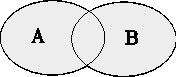
\includegraphics{img/vereinigung.pdf} &
 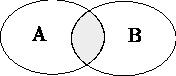
\includegraphics{img/durchschnitt.pdf} &
 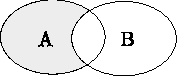
\includegraphics{img/differenz.pdf} \\
 Vereinigung & Durchschnitt & Differenz \\
 $A \cup B$ & $A \cap B$ & $A \setminus B$
\end{tabular}

\vspace{1em}\par

\emph{$a$ ist Element von $A$}: $a\in A$.

Die \emph{leere Menge} ($\emptyset$) ist die Menge, die keine Elemente hat.

Zwei Mengen sind gleich ($A=B$), wenn beide aus den selben Elementen bestehen.

\begin{itemize}
\item Zwei Mengen heißen \emph{disjunkt}, wenn sie keine gemeinsamen Elemente haben:
$A\cap B = \emptyset$.

\item Eine Menge $A$ kann vollständig in einer anderen Menge $B$ enthalten sein: 
$A\subseteq B$ (sprich: \emph{$A$ ist eine Teilmenge von $B$}). Wenn $A\neq B$ 
gilt, ist $A$ eine \emph{echte Untermenge} von $B$ ($A \subset B$).

\item Analog ist definiert: $A$ ist eine (echte) Obermenge von $B$: $A \supseteq B$ 
($A \supset B$).

\item Die \emph{Komplementmenge} $\overline{A}$ der Menge $A$ enthält alle Elemente,
die in $A$ nicht enthalten sind. Wenn $A$ eine Teilmenge einer Trägermenge $X$
ist, dann gilt: $\overline{A} = X\setminus A$

\end{itemize}

\begin{table}
\begin{tabular}{cclp{17em}}
\textbf{klein} & \textbf{groß} & \textbf{Name} & \textbf{übliche Verwendung}\\
\hline
$\alpha$& & Alpha & Winkel\\
$\beta$ & & Beta & Winkel\\
$\gamma$ & $\Gamma$ & Gamma & \\
$\delta$ & $\Delta$ & Delta & $\Delta$: Differenz\\
$\varepsilon$ & & Epsilon & sehr kleine positive Zahl\\
$\eta$ & & Eta\\
$\theta$ & $\Theta$ &  Theta & $\theta$: Winkel in Polarkoordinaten\\
$\lambda$ & &  Lambda & multiplikativer Faktor\\
$\mu$ & & My\\
$\xi$ & & Xi \\
$\pi$ & $\Pi$ & Pi & $\pi = 3,14\dots$, $\Pi$: Multiplikation\\
$\rho$ & & Rho\\
$\sigma$ & $\Sigma$ & Sigma & $\Sigma$: Summe\\
$\tau$ & & Tau \\
$\phi$ & $\Phi$ & Phi & $\phi$: Winkel \\
$\chi$ & & Chi \\
$\psi$ & $\Psi$ & Psi \\
$\omega$ & $\Omega$ & Omega\\
\end{tabular}
\label{tab:griechisch}
\caption{Auswahl von wichtigen griechischen Buchstaben}
\end{table}


\section{Intervalle}
Ein Intervall ist ein zusammenhängender Zahlenbereich, der durch seine beiden
Endpunkte bestimmt ist. Es wird zwischen geschlossenen und
offenen Intervallen unterschieden. Ein \emph{geschlossenes Intervall}
$[a,b]$ enthält $a$ und $b$ (inklusiv), ein \emph{offenes Intervall}
$(a,b)$ enthält $a$ und $b$ nicht mehr (exklusiv).

Es ist möglich, beide Arten zu kombinieren. Es entsteht ein
\emph{halboffenes Intervall}: $[a,b)$ enthält $a$, aber nicht $b$, während
$(a,b\,]$ hingegen $b$, aber nicht $a$ enthält.

\begin{table}[htb]
\begin{tabular}{ll}
\textbf{Symbol} & \textbf{Bedeutung}\\\hline
 $\exists x$    & es existiert (mindestens) ein $x$\\
 $\nexists x$   & es existiert kein  $x$\\
 $\forall x$    & für alle $x$ gilt \dots\\
 $\pm$          & Plus/Minus, z.\,B. $x_{1,2} = \pm 1 \rightarrow x_1 = -1,
x_2 = +1$\\
 $\sum\limits_{i=1}^n a_i$ & $a_1 + a_2 + \dots  + a_n$ \\
 $\prod\limits_{i=1}^n a_i$ & $a_1 \cdot a_2 \cdot\  \cdots\ \cdot a_n$\\
 $\infty$       & Unendlich \\
 $\wedge$       & logisches und\\
 $\vee$         & logisches oder\\
 $\neg$         & logische Negation\\
 $:=$           & ist definiert als\\
 $<,\leq$       & kleiner als, kleiner oder gleich (oft auch: \glqq echt
kleiner, kleiner\grqq)\\
 $>,\geq$       & größer als, größer oder gleich (oft auch: \glqq echt
größer, größer\grqq)\\
 $=, \neq$      & gleich, ungleich\\
\end{tabular}
\label{tab:zeichen}
\caption{Wichtige Sonderzeichen}
\end{table} 


\section{Abkürzungen und Vokabeln}
\begin{description}
 \item[gdw.] Kurz für \glqq genau dann, wenn\grqq. Als Symbol wird auch
$\Leftrightarrow$ verwendet.
 \item[qed] Am Ende eines Beweises. Lateinisch \glqq quod erat
demonstrandum\grqq{} (\glqq was zu zeigen/ beweisen war\grqq). Bedeutung:
Hurra, wir haben den Beweis endlich hinter uns. Gedruckt wird auch
das Zeichen $\square$ verwendet.
 \item[kommutativ] \glqq vertauschbar\grqq. Eine Operation (z.B. $+,\cdot$)
ist kommutativ, wenn man die beiden Operanden vertauschen kann, ohne das
Ergebnis zu ändern. Als Formel ausgedrückt, heißt das: $a\circ b = b\circ a$,
wobei $\circ$ für die Operation steht.
 \item[distributiv] Ausklammern ist erlaubt: $a\cdot(b+c) = a\cdot b + a\cdot
c$
 \item[assoziativ] Die Reihenfolge, in der die Operation durchgeführt wird,
ist beliebig: $a+b+c = (a+b)+c = a+(b+c)$.
 \item[es existiert ein] Es gibt \emph{mindestens} ein Element, das die
Aussage erfüllt.
 \item[es existiert genau ein] Es gibt nur ein einziges Element, das die
Aussage erfüllt.
 \item[notwendige Bedingung] Diese Bedingung ist immer erfüllt, falls eine Aussage gilt. Es gibt aber auch Fälle, in denen die Bedingung erfüllt ist, obwohl die Aussage nicht gilt.
 \item[hinreichende Bedingung] Wenn diese Bedingung erfüllt ist, gilt die Aussage auf jeden Fall. Es gibt aber Fälle, in denen die Aussage gilt, die Bedingung aber nicht erfüllt ist.
 \item[notwendige und hinreichende Bedingung] Immer dann, wenn diese Bedingung erfüllt ist, gilt auch die Aussage (und umgekehrt).
\end{description}

%\pagebreak

%\section{Wichtige griechische Buchstaben}
%Tabelle~\ref{tab:griechisch} enthält eine Auswahl mit Buchstaben, denen du begegnen
%wirst, und ihre übliche Verwendung.

%\section{Komische Zeichen}
%Tabelle~\ref{tab:zeichen} enthält eine Übersicht der wichtigsten mathematischen Zeichen.


\chapter{Basismathematik}
\addtocontents{toc}{\setcounter{tocdepth}{1}}

\section{Bruchrechnung}
\label{Bruchrechnung}
Autor: Katja Matthes
%%%%%%%%%%%%%%%%%%%%%%%%%%%%%%%%%%%%%%%%%%%%%%%%%%%%%%%%%%%%%%%%%%%%
%%%Definition
%%%%%%%%%%%%%%%%%%%%%%%%%%%%%%%%%%%%%%%%%%%%%%%%%%%%%%%%%%%%%%%%%%
\subsection{Definition}
Ein Bruch ist die Darstellung einer rationalen Zahl als Quotient.

\qquad Bruch: $\frac{Z}{N}$ \qquad mit $Z \in \mathbb{Z}$ und $N \in \mathbb{Z}\setminus\{0\} $
	
\qquad Z\ \ldots\ Zähler \qquad N\ \ldots\ Nenner
	
Zwei Brüche $\frac{a}{b}$ und $\frac{c}{d}$ hei\ss en gleichnamig, wenn sie den gleichen Nenner haben: $b = d$.

%%%%%%%%%%%%%%%%%%%%%%%%%%%%%%%%%%%%%%%%%%%%%%%%%%%%%%%%%%%%%%%%%%%%
%%%K�rzen und Erweitern
%%%%%%%%%%%%%%%%%%%%%%%%%%%%%%%%%%%%%%%%%%%%%%%%%%%%%%%%%%%%%%%%%%
\subsection{Kürzen und Erweitern}
Ein Bruch wird gekürzt, indem sowohl Nenner als auch Zähler durch die gleiche Zahl dividiert werden.
\[ \frac{a \cdot c}{b \cdot c} \stackrel{: c}{=} \frac{a}{b}\]
Ein Bruch wird erweitert, indem sowohl Nenner wie Zähler mit dem gleichen Faktor multipliziert werden.
\[ \frac{a}{b} \stackrel{\cdot c}{=}  \frac{a \cdot c}{b \cdot c} \]
	
%%%%%%%%%%%%%%%%%%%%%%%%%%%%%%%%%%%%%%%%%%%%%%%%%%%%%%%%%%%%%%%%%%%%
%%%spezielle Rechenregeln
%%%%%%%%%%%%%%%%%%%%%%%%%%%%%%%%%%%%%%%%%%%%%%%%%%%%%%%%%%%%%%%%%%
\subsection{Spezielle Rechenregeln}
\subsubsection{Addition von gleichnamigen Brüchen}
Zwei gleichnamige Brüche werden addiert, indem ihre Zähler addiert werden und der Nenner übernommen wird.
	\[\frac{a}{b} + \frac{c}{b} = \frac{a+c}{b}\]
	
\subsubsection{Subtraktion von gleichnamigen Brüchen}
Zwei gleichnamige Brüche werden subtrahiert, indem ihre Zähler subtrahiert werden und der Nenner beibehalten wird.
	\[\frac{a}{b} - \frac{c}{b} = \frac{a-c}{b}\]
	
\subsubsection{Multiplikation mit einem Faktor}
Ein Bruch wird mit einem Faktor $n$ multipliziert, indem der Zähler mit diesem Faktor multipliziert wird, während der Nenner übernommen wird.
	\[\frac{a}{b} \cdot n = \frac{a \cdot n}{b}\]
	
\subsubsection{Division durch eine Zahl}
Ein Bruch wird durch eine Zahl $n \neq 0$ dividiert, indem der Nenner mit dieser Zahl multipliziert wird und der Zähler beibehalten wird.
	\[\frac{a}{b} : n = \frac{a}{b \cdot n}\]

%%%%%%%%%%%%%%%%%%%%%%%%%%%%%%%%%%%%%%%%%%%%%%%%%%%%%%%%%%%%%%%%%%%%
%%%allgemeine Rechenregeln
%%%%%%%%%%%%%%%%%%%%%%%%%%%%%%%%%%%%%%%%%%%%%%%%%%%%%%%%%%%%%%%%%%	
\subsection{Allgemeine Rechenregeln}
\subsubsection{Addition}
Zwei Brüche werden addiert, indem sie zunächst gleichnamig gemacht werden und dann die Zähler addiert werden.
	\[\frac{a}{b} + \frac{c}{d} = \frac{a \cdot d}{b \cdot d} + \frac{b \cdot c}{b \cdot d} = \frac{a \cdot d + b \cdot c}{b \cdot d} \]
	
\subsubsection{Subtraktion}
Zwei Brüche werden subtrahiert, indem sie zunächst gleichnamig gemacht werden und dann die Zähler subtrahiert werden.
	\[\frac{a}{b} - \frac{c}{d} = \frac{a \cdot d}{b \cdot d} - \frac{b \cdot c}{b \cdot d} = \frac{a \cdot d - b \cdot c}{b \cdot d} \] 
	
\subsubsection{Multiplikation}
Zwei Brüche werden mulipliziert, indem jeweils die Nenner und Zähler multipliziert werden.
	\[\frac{a}{b} \cdot \frac{c}{d} = \frac{a \cdot c}{b \cdot d}\]

\subsubsection{Division}
Ein Bruch wird durch einen anderen dividiert, indem er mit dessen Kehrwert multipliziert wird.
\[\frac{a}{b} : \frac{c}{d} = \frac{a}{b} \cdot \frac{d}{c} = \frac{a \cdot d}{b \cdot c}\] 

%%%%%%%%%%%%%%%%%%%%%%%%%%%%%%%%%%%%%%%%%%%%%%%%%%%%%%%%%%%%%%%%%%%%
%%%Literatur
%%%%%%%%%%%%%%%%%%%%%%%%%%%%%%%%%%%%%%%%%%%%%%%%%%%%%%%%%%%%%%%%%%
\subsection{Literatur}
\begin{itemize}
	\item Formeln und Tabellen für die Sekundarstufen I und II. 7. Aufl. - Berlin: Paetec, Ges. für Bildung und Technik, 1999
\end{itemize}

%%%%%%%%%%%%%%%%%%%%%%%%%%%%%%%%%%%%%%%%%%%%%%%%%%%%%%%%%%%%%%%%%%%%
%%%Aufgaben
%%%%%%%%%%%%%%%%%%%%%%%%%%%%%%%%%%%%%%%%%%%%%%%%%%%%%%%%%%%%%%%%%%
%\newpage
\subsection{Aufgaben}

\subsubsection{Aufgabe 1}
Kürze soweit möglich.
\begin{enumerate}
\begin{multicols}{4}
	\item \quad $ \frac{20}{6} $
	\item \quad $ \frac{92}{4} $
	\item \quad $ \frac{360}{25} $
	\item \quad $ \frac{1716}{308} $
\end{multicols}
\end{enumerate}

\subsubsection{Aufgabe 2}
Berechne und kürze soweit wie möglich.
\begin{enumerate}
\begin{multicols}{2}
	\item \quad $ \frac{56}{65} \cdot 12 \cdot \frac{5}{7} \cdot \frac{13}{16} $
	\item \quad $ 1 : \left( \frac{2}{9} + \frac{1}{7} \right) $
	\item \quad $ \left( \frac{3}{5} - \frac{1}{4} \right) : \frac{3}{4} $
\end{multicols} 
\end{enumerate}

\subsubsection{Aufgabe 3}
Berechne.
\begin{enumerate}
\begin{multicols}{4}
	\item \quad $ \frac{\frac{8}{9}}{\frac{16}{27}} $
	\item \quad $ \frac{2\frac{1}{3}}{1\frac{1}{6}} $
	\item \quad $ \frac{5\frac{1}{2}}{\frac{11}{12}} $
	\item \quad $ \frac{\frac{99}{100}}{\frac{9}{10}} $
\end{multicols} 
\end{enumerate}

\subsubsection{Aufgabe 4}
Berechne.
\begin{enumerate}
	\item \quad $ \frac{5}{6} \cdot \frac{2}{3} - \frac{2}{9} + \frac{3}{4} \cdot 1\frac{7}{9} $
	\item \quad $ 3\frac{5}{12} - 2\frac{5}{6} + 1\frac{1}{3} : \frac{4}{9} - 2\frac{1}{6} \cdot \frac{1}{2} $
\end{enumerate}

\subsubsection{Aufgabe 5}
Berechne.
\begin{enumerate}
\begin{multicols}{2}
	\item \quad $ \left(\frac{2}{3} - \frac{1}{6}\right) \cdot \left(\frac{9}{11} - \frac{3}{7}\right) $
	\item \quad $	\left(\frac{1}{8} + \frac{7}{12}\right) : \left(5 - \frac{3}{4}\right) $
	\item \quad $ \frac{4}{7} \cdot \left(\left(1\frac{1}{2} - \frac{5}{9}\right) : 4\frac{1}{4}\right) $
	\item \quad $ \frac{4}{5} : \left[\left(\frac{5}{8} - \frac{1}{3}\right) \cdot 12\right] $
	\item \quad $ \frac{3}{4} \cdot \left(2\frac{1}{2} : 1\frac{1}{4}\right) $
\end{multicols} 
\end{enumerate}

\subsubsection{Aufgabe 6}
Berechne.
\begin{enumerate}
\begin{multicols}{2}
	\item \quad $ \frac{\frac{3}{8} \cdot \frac{2}{7}}{\frac{5}{14}} $
	\item \quad $ \frac{1\frac{3}{4} + \frac{5}{6}}{\frac{1}{4}} $
	\item \quad $ \frac{\frac{8}{9}}{3\frac{1}{3} + \frac{1}{6}} $
	\item \quad $ \frac{\left(\frac{3}{5} - \frac{5}{10}\right) : \frac{2}{5}}{\frac{1}{4} + \frac{1}{2}} $
\end{multicols}
\end{enumerate}


\section{Potenzen}
\label{Potenzen}
Autor: Katja Matthes
%%%%%%%%%%%%%%%%%%%%%%%%%%%%%%%%%%%%%%%%%%%%%%%%%%%%%%%%%%%%%%%%%%%%
%%%Definition
%%%%%%%%%%%%%%%%%%%%%%%%%%%%%%%%%%%%%%%%%%%%%%%%%%%%%%%%%%%%%%%%%%
\subsection{Definition}
Potenzen sind eine abkürzende Schreibweise für eine wiederholte Multiplikation mit einem Faktor.
   \[ \begin{matrix} \underbrace{ a\cdot a\cdot a\cdots a }&=a^n\\{n\ \mathrm{Faktoren}} \end{matrix} \]
\begin{multicols}{3}
	$ a^n $ \ldots\ Potenz \\
  $ a $ \ldots\ Basis\\
  $ n $ \ldots\ Exponent
\end{multicols}
%%%%%%%%%%%%%%%%%%%%%%%%%%%%%%%%%%%%%%%%%%%%%%%%%%%%%%%%%%%%%%%%%%%%
%%%Besondere Exponenten
%%%%%%%%%%%%%%%%%%%%%%%%%%%%%%%%%%%%%%%%%%%%%%%%%%%%%%%%%%%%%%%%%%
\subsection{Besondere Exponenten}
Seien $ a \in \mathbb{R}\setminus\{0\} $ und $ n \in \mathbb{N}_{0} $, dann gilt:
\begin{align*}
    a^0 &= 1 \\
    a^1 &= a \\
    a^{-n} &= \frac{1}{a^n} 
\end{align*}
%%%%%%%%%%%%%%%%%%%%%%%%%%%%%%%%%%%%%%%%%%%%%%%%%%%%%%%%%%%%%%%%%%%%
%%%Potenzgesetze
%%%%%%%%%%%%%%%%%%%%%%%%%%%%%%%%%%%%%%%%%%%%%%%%%%%%%%%%%%%%%%%%%%
\subsection{Potenzgesetze}
Folgende \textbf{Potenzgesetze} gelten für alle $ m $, $ n \in \mathbb{Z} $ und $ a$, $ b \in \mathbb{R}\setminus\{0\} $.
%%%%%%%%%%%%%%%%%%%%%%%%%%%%%%%%%%%%%%%%%%%
\begin{enumerate}
	\item %%%%%%%%%%% 1. %%%%%%%%%%%%%%%%%
		Potenzen mit gleicher Basis werden multipliziert, indem die Basis beibehalten wird und die Exponenten addiert werden.
		\[a^m \cdot a^n = a^{m+n}\]
	\item %%%%%%%%%%% 2. %%%%%%%%%%%%%%%%%
		Potenzen mit gleicher Basis werden dividiert, indem die Basis beibehalten wird und die Exponenten subtrahiert werden.	
		\[\frac{a^m}{a^n} = a^{m-n}\]
	\item %%%%%%%%%%% 3. %%%%%%%%%%%%%%%%%
		Potenzen mit gleichem Exponenten werden multipliziert, indem die Basen multipliziert werden und der Exponent beibehalten wird.
		\[a^n \cdot b^n = (a \cdot b)^n\]
	\item %%%%%%%%%%% 4. %%%%%%%%%%%%%%%%%
		Potenzen mit gleichem Exponenten werden dividiert, indem die Basen dividiert werden und der Exponent beibehalten wird.
		\[\frac{a^n}{b^n} = \left(\frac{a}{b}\right)^n\]
	\item %%%%%%%%%%% 5. %%%%%%%%%%%%%%%%%
		Potenzen werden potenziert, indem die Basis beibehalten wird und die Exponenten multipliziert werden.
		\[(a^m)^n = a^{m \cdot n} = (a^n)^m \]
\end{enumerate}
%%%%%%%%%%%%%%%%%%%%%%%%%%%%%%%%%%%%%%%%%%%%%%%%%%%%%%%%%%%%%%%%%%%%
%%%Wurzeln
%%%%%%%%%%%%%%%%%%%%%%%%%%%%%%%%%%%%%%%%%%%%%%%%%%%%%%%%%%%%%%%%%%
\subsection{Wurzeln}
Seien $ m $, $ n \in \mathbb{N} $ und $ a \in \mathbb{R} $ mit $ a>0 $, dann gilt:
	\[a^{\frac{m}{n}} = \sqrt[n]{a^m}\]
Damit sind die Potenzgesetze auch auf Wurzeln anzuwenden.
\noindent Man nennt $a$ den Radikanten und $n$ den Wurzelexponenten.
%%%%%%%%% Wurzelgesetzte %%%%%%%%%%%%%%%%%%%%%%%%%%%%%
\subsection{Wurzelgesetze}
Für $m$, $n \in \mathbb{N}_{>1}$ und nichtnegativen reelen Radikanden $a$ und $b$ gilt:
\begin{enumerate}
	\item $\sqrt[m]{a}\cdot\sqrt[n]{a} = \sqrt[mn]{a^{m+n}}$
	\item $\frac{\sqrt[m]{a}}{\sqrt[n]{a}} = \sqrt[mn]{a^{n-m}}$
	\item $\sqrt[n]{a}\cdot\sqrt[n]{b} = \sqrt[n]{a\cdot b}$
	\item $\frac{\sqrt[n]{a}}{\sqrt[n]{b}} = \sqrt[n]{\frac{a}{b}}$
	\item $\sqrt[n]{\sqrt[m]{a}} = \sqrt[mn]{a} = \sqrt[m]{\sqrt[n]{a}}$
\end{enumerate} 
%%%%%%%%%%%%%%%%%%%%%%%%%%%%%%%%%%%%%%%%%%%%%%%%%%%%%%%%%%%%%%%%%%%%
%%%Literatur
%%%%%%%%%%%%%%%%%%%%%%%%%%%%%%%%%%%%%%%%%%%%%%%%%%%%%%%%%%%%%%%%%%
\subsection{Literatur}
\begin{itemize}
	\item http://de.wikipedia.org/wiki/Potenzen
	\item Formeln und Tabellen für die Sekudarstufen I und II. 7. Aufl. - Berlin: Paetec, Ges. für Bildung und Technik, 1999
\end{itemize}
%%%%%%%%%%%%%%%%%%%%%%%%%%%%%%%%%%%%%%%%%%%%%%%%%%%%%%%%%%%%%%%%%%%%
%%%Aufgaben
%%%%%%%%%%%%%%%%%%%%%%%%%%%%%%%%%%%%%%%%%%%%%%%%%%%%%%%%%%%%%%%%%%
\pagebreak
\subsection{Aufgaben}

\subsubsection{Aufgabe 1}
Vereinfache.
\begin{enumerate}
\begin{multicols}{2}
	\item \quad $ 3x^4 - x^4 - x^3(x + 2) $
	\item \quad $ -12a^2 + 3a(a + 1) $
	\item \quad $ ax^n + 4x^n $
	\item \quad $ (1-t)^2 - \frac{1}{2}(1-t)^2 $
	\item \quad $ a(x+t)^k - b(x+t)^k $
	\item \quad $ tx^3 - 3x^2 + 2tx^3 - 4x^2 $
	\item \quad $ t^3 \cdot t^4 - t^5(t^2+1) $
	\item \quad $ x^2 \cdot x^3 \cdot x^4 $
	\item \quad $ 3a^k \cdot a^{k-1} \cdot a $
	\item \quad $ b^n \cdot b^{2n+1} $
	\item \quad $ (x+1)^{n-1} \cdot (x+1)^{n+1} $
	\item \quad $ \left(\frac{x}{3}\right)^4 \cdot \left(\frac{x}{3}\right)^2 $
	\item \quad $ t^2 \cdot x^2 \cdot t^n \cdot x^{n-1} $
	\item \quad $ a \cdot b^k \cdot a^{2n} \cdot b^{k-3} $
	\item \quad $ (x-2)^n \cdot (x-2)^{1-n} $
	\item \quad $ 0,3^6 \cdot \left(\frac{10}{3}\right)^6 $
	\item \quad $ 2^x \cdot \left(\frac{5}{2}\right)^x \cdot 5 $
	\item \quad $ 2^5 \cdot \left(\frac{1}{2}\right)^4 $
	\item \quad $ \left(\frac{x}{4}\right)^4 \cdot 4^6 $
	\item \quad $ 2^n \cdot \left(\frac{x}{2}\right)^n \cdot x $
	\item \quad $ 9 \cdot 3^{n+1} $
	\item \quad $ (a-b)^9 \cdot (a-b) $
	\item \quad $ \left(\frac{a-b}{c}\right)^{2k} \cdot \left(\frac{c}{a-b}\right)^{2k} $
\end{multicols}
\end{enumerate}

%\newpage

\subsubsection{Aufgabe 2}
Vereinfache.
\begin{enumerate}
\begin{multicols}{2}
	\item \quad $ \frac{a^6}{a^3} $
	\item \quad $ \frac{x^{2n+1}}{x^n} $
	\item \quad $ \frac{15e^{x+1}}{5e^x} $
	\item \quad $ \frac{x^4}{x^7} $
	\item \quad $ \frac{2a^{1-2n}}{4a^{n+1}} $
	\item \quad $ \frac{a^4b^{4n+3}}{a^nb^{2n-1}} $
	\item \quad $ \frac{81}{3^{x+3}} $
	\item \quad $ \frac{(a-b)^3}{(a-b)^{n-1}} $
	\item \quad $ \frac{(ab)^3}{x^2y} \cdot \frac{(xy)^2}{a^4b^2} $
	\item \quad $ \frac{a^{n+1}}{a^n} $
	\item \quad $ \frac{10^3}{2^3} $
	\item \quad $ \frac{2,5^4}{0,5^4} $
	\item \quad $ \frac{(10ab)^k}{(4b)^k} $
	\item \quad $ \left(\frac{a}{b}\right)^n \cdot \frac{a}{b} $
	\item \quad $ \left(\frac{-1}{a-b}\right)^3 $
	\item \quad $ \left(\frac{x}{2}\right)^3 : \left(\frac{x}{3}\right) $
	\item \quad $ (-5^2)^3 $
	\item \quad $ 3(c^4)^3 - 6c^{12} $
	\item \quad $ (3b^2c^{n-1})^4 $
	\item \quad $ \left(\frac{7a^2}{49b^3}\right)^2 $
	\item \quad $ \left(\frac{-1}{c^3}\right)^{2n} $
	\item \quad $ (3b^{n+1} \cdot c^{n-1})^2 $
	\item \quad $ (x^2y^3z^2)^5 $
	\item \quad $ (0,5e^{x+2})^2 $
	\item \quad $ \left(\frac{2}{x^2}\right)^5 - \left(\frac{3}{x^5}\right)^2 $
	\item \quad $ \left[\left(-\frac{3}{t}\right)^3\right]^4 \cdot \frac{t^9}{81} $
	\item \quad $ \frac{(ab)^2}{x^3y} \cdot \frac{x^5y^2}{a^2b} $
	\item \quad $ \frac{(4-12x)^3}{64} $
	\item \quad $ \frac{(2x-4)^5}{(2-x)^3} $
	\item \quad $ \frac{(4ab)^4}{(6a^2)^4} \cdot \frac{5}{b^4} $
	\item \quad $ (a-b^2) \cdot (a-b^2)^n $
\end{multicols}
\end{enumerate}

\subsubsection{Aufgabe 3}
Vereinfache.
\begin{enumerate}
	\item \quad $ \left(\frac{1}{2}x^2\right)^5 + \frac{1}{8}(x^2)^5 + (2x^5)^2 $
	\item \quad $ \frac{1}{4} \cdot 2^4(2^2)^3 $
	\item \quad $ (3^{n+1})^2 $
	\item \quad $ (3x^2 - 5x)(1-x^3) + (x^2 + 3x^4)x^3 $
	\item \quad $ a^{2r}b^r(a^{2r} - a^rb^{r+1} + b^{2r+2}) $
\end{enumerate}

\subsubsection{Aufgabe 4}
Vereinfache.
\begin{enumerate}
\begin{multicols}{2}
	\item \quad $ -3x^3 \cdot x^2 + 5x \cdot x^4 $
	\item \quad $ 4t^{n-4}t^3-t \cdot t^{n-2} $
	\item \quad $ 2x^5y^3y - 4x^3y^2x^2y^2 $
	\item \quad $ \frac{4x^5 + 6x^4 -12x^2}{2x^2} $
	\item \quad $ (9 \cdot 3^n - 3^{n+1}) : 3^{n-1} $
	\item \quad $ (2x+6)^2+(x+3)^2 $
	\item \quad $ \frac{5a-20}{4a-16} $
	\item \quad $ (3t^2 - 3t^3)^2 $
\end{multicols}
\end{enumerate}

\newpage

\subsubsection{Aufgabe 5}
Faktorisiere - Schreibe als Produkt durch Ausklammern.
\begin{enumerate}
\begin{multicols}{2}
	\item \quad $ 3a^2 + 6a^3 $
	\item \quad $ \frac{1}{2}e^x - \frac{1}{4}e^{x+1} $
	\item \quad $ a^{5b} + 3a^b $
	\item \quad $ 2^x + 2^{x+1} $
	\item \quad $ x^4+2x^3 $
	\item \quad $ x^{n+3} - 4x^{n+2} $
	\item \quad $ -6t^{n+2}+18t^{2-n} $
	\item \quad $ e^x-e^{3x} $
\end{multicols}
\end{enumerate}

\subsubsection{Aufgabe 6}
Vereinfache.
\begin{enumerate}
\begin{multicols}{2}
	\item \quad $ \frac{x^4-x^3}{x^2-x} $
	\item \quad $ \frac{e^{3x}+e^{2x}}{e^{2x}} $
	\item \quad $ \frac{a^7b^3-ab^7}{a^5b-a^2b^4} $
	\item \quad $ \frac{32}{2^{n+5}} + \frac{2^{-n+3}}{8} $
\end{multicols}
\end{enumerate}

\subsubsection{Aufgabe 7}
Berechne y.
\begin{enumerate}
	\item \quad $ y = \frac{1}{4}x^4-2tx^3+\frac{9}{2}t^2x^2 $ mit $ x = 3t $
	\item \quad $ y = e^{x^2-t^2}+3e^{5t-(t-x)} $ mit $ x = -t $
	\item \quad $ y = \frac{3}{2t^2}x^4 - \frac{4}{t}x^3 + 3x^2 - 4 $ mit $ x = \frac{1}{3}t $
	\item \quad $ y = \frac{e^{3tx}+4e^3}{tx-4} $ mit $ x = \frac{1}{t} $
	\item \quad $ y = \frac{tx^3}{2(x+t)^2} $ mit $x = -3t $ 
\end{enumerate}

\subsubsection{Aufgabe 8}
Klammere aus.
\begin{enumerate}
	\item \quad $ a^n+a^{4-n}+a^{2n} = a^{2n}(\ldots) $
	\item \quad $ a^3 + a^{1-n} + a^{n+4} = a^{n+3}(\ldots) $
	\item \quad $ \frac{3}{2}x^4+\frac{3}{4}x^3+\frac{1}{8}x^2 = \frac{1}{8}x^2(\ldots) $
	\item \quad $ e^{3x}-2e^{-x} = e^{-x}(\ldots) $
	\item \quad $ te^{2x}-2e^{x+1} = e^x(\ldots) $
\end{enumerate}

\subsubsection{Aufgabe 9}
Multipliziere aus und vereinfache.
\begin{enumerate}
\begin{multicols}{2}
	\item \quad $ \frac{1}{4} \cdot 2^{-4} \cdot (2^2)^3 $
	\item \quad $ (e^x - e^{-x} + 5)e^x $
	\item \quad $ 2^x(2^{-1}+2^x) $
	\item \quad $ (x^4+x^{-2})(x^3-x^{-3}) $
\end{multicols}
\end{enumerate}

\subsubsection{Aufgabe 10}
Vereinfache/Fasse zusammen.
\begin{enumerate}
\begin{multicols}{2}
	\item \quad $ a^2 \cdot (a^2)^{-2} + 3a \left(\frac{1}{a}\right)^3 $
	\item \quad $ \frac{1}{18} \cdot (3^2)^2 + \frac{1}{2} \cdot 3^3 \cdot \left(\frac{1}{3}\right)^2 $
	\item \quad $ (x^2 \cdot x^{-3})^{-2} + \left(\frac{3}{x^2}\right)^{-1} $
	\item \quad $ a^5 \cdot a^{-2} + 4a^2 \cdot a $
	\item \quad $ \left(\frac{2}{x}\right)^3 + \left(\frac{1}{x}\right)^3 $
	\item \quad $ \frac{1}{e^{2x}} + 3(e^{-x})^2 - \left(\frac{2}{e^x}\right)^2 $
	\item \quad $ e^{-x} \cdot e^{-x+2} \cdot e^{2x-3} $
	\item \quad $ 6x^3 \cdot x^{-1} - 8x^4 \cdot x^{-2} $
	\item \quad $ (t^7-t^4) \cdot t^{-3} $
\end{multicols}
\end{enumerate}
	
\subsubsection{Aufgabe 11}
Vereinfache/Fasse zusammen.
\begin{enumerate}
\begin{multicols}{2}
	\item \quad $ \frac{-2^3 - 2 \cdot 4}{2 \cdot 2^3} $
	\item \quad $ \frac{(1-x)^2}{(x-1)} $
	\item \quad $ \frac{e^{3x+1}}{e^{-x+2}} $
	\item \quad $ \frac{1,5e^{3x} - e^x}{1,5e^{3x}} $
\end{multicols}
\end{enumerate}

\subsubsection{Aufgabe 12}
Vereinfache/Fasse zusammen.
\begin{enumerate}
	\item \quad $ a^4 \cdot a^{-6} - 3a^3 \cdot a^{-5} + a^2 $
	\item \quad $ (a^{n+2} - 4a^n - 2a^{2-n})\cdot \frac{a^{-2}}{2} $
	\item \quad $ 4x^{-4}x^7 - 0,5 x^4x^{-1} + \left(\frac{1}{x^2}\right)^{1,5} $
	\item \quad $ \frac{a^{n+1}}{a} + \frac{a^{2n-1}}{a^{n+2}} + (a^{n-1})^2 \cdot a^{2-n} $
	\item \quad $ \frac{2^{2k}}{8} \cdot 2^{3-k} + 2 \cdot 2^{k-1} $
\end{enumerate}

\newpage

\subsubsection{Aufgabe 13*}
Vereinfache. (Tipp: Mache eine Fallunterscheidung.)
\begin{enumerate}
\begin{multicols}{2}
	\item \quad $ (a-b)^n + (b-a)^n $
	\item \quad $ (x-2)^n + (2x-4)^n - (2-x)^n $
\end{multicols}
\end{enumerate}
\section{Binomische Formeln}
\label{binomisch}
Autor: Katja Matthes
%%%%%%%%%%%%%%%%%%%%%%%%%%%%%%%%%%%%%%%%%%%%%%%%%%%%%%%%%%%%%%
%%%Definition
%%%%%%%%%%%%%%%%%%%%%%%%%%%%%%%%%%%%%%%%%%%%%%%%%%%%%%%%%%%%%%
\subsection{Definition}
Die Binomischen Formeln sind Formeln zur Darstellung und zum Lösen von Quadrat-Binomen. Sie erleichtern das Ausmultiplizieren von Klammer"-aus"-drü"-ck"-en und erlauben Term-Umformungen von bestimmten Summen und Differenzen in Produkte. Dies stellt sehr oft die einzige Lösungsstrategie bei der Vereinfachung von Bruchtermen, beim Radizieren von Wurzeltermen sowie Logarithmenausdrücken dar.
%%%%%%%%%%%%%%%%%%%%%%%%%%%%%%%%%%%%%%%%%%%%%%%%%%%%%%%%%%%%%%
%%%Formeln
%%%%%%%%%%%%%%%%%%%%%%%%%%%%%%%%%%%%%%%%%%%%%%%%%%%%%%%%%%%%%%
\subsection{Formeln}
%%%%%%%%%%%%%%%%%%%%%%%%%%%%%%%%%%%%%%%%%%%%%%%%%%%%%%%%%%%%%%
%%%1. Binomische Formeln
%%%%%%%%%%%%%%%%%%%%%%%%%%%%%%%%%%%%%%%%%%%%%%%%%%%%%%%%%%%%%%
\subsubsection{Erste binomische Formel}
	\[(a + b)^2 = a^2 + 2ab + b^2\]
Die erste binomische Formel kann wie im folgenden Bild dargestellt werden:
\begin{center}
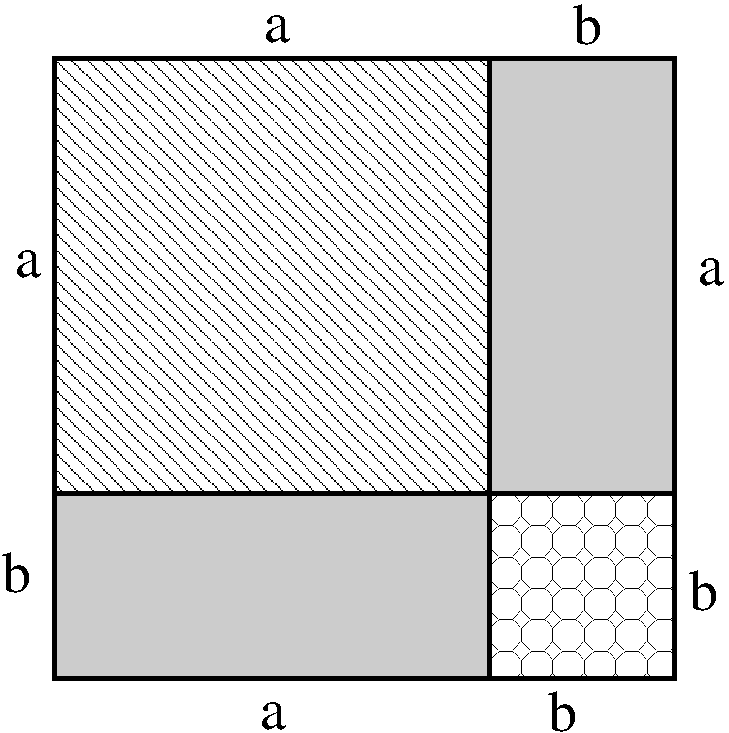
\includegraphics[height=3cm]{img/binF1.pdf}
\end{center}
Die Fläche eines Quadrates entspricht seiner Seitenlänge zum Quadrat. In der Abbildung beträgt die Seitelänge des Quadrats $ (a+b) $. Dementsprechend ist der Flächeninhalten des gesamten Quadrates $ (a+b)^2 $.

Die gleiche Fläche entsteht auch, indem ein schraffiertes Quadrat (Fläche: $ a^2 $), zwei graue Rechtecke (Fläche: $ 2\cdot ab $) und ein gekringeltes Quadrat (Fläche: $ b^2 $) zusammen gelegt werden. Es ergibt sich also folgende Legende: 
\begin{center}
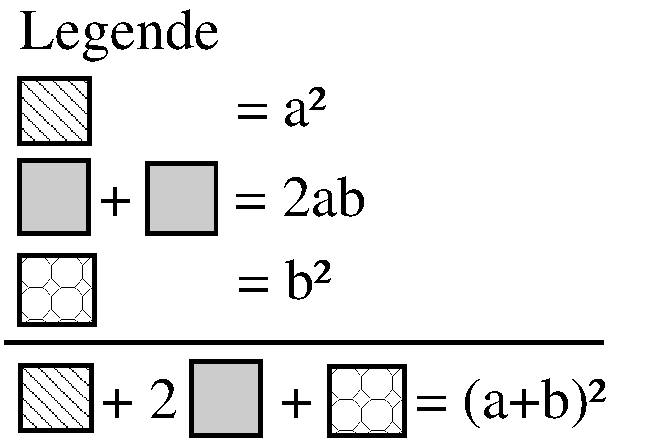
\includegraphics[height=2cm]{img/binF1legende.pdf}
\end{center}
%%%%%%%%%%%%%%%%%%%%%%%%%%%%%%%%%%%%%%%%%%%%%%%%%%%%%%%%%%%%%%
%%%2. Binomische Formeln
%%%%%%%%%%%%%%%%%%%%%%%%%%%%%%%%%%%%%%%%%%%%%%%%%%%%%%%%%%%%%%
\subsubsection{Zweite binomische Formel}
	\[(a - b)^2 = a^2 - 2ab + b^2\]
Die zweite binomische Formel kann durch folgende Abbildung veranschaulicht werden:
\begin{center}
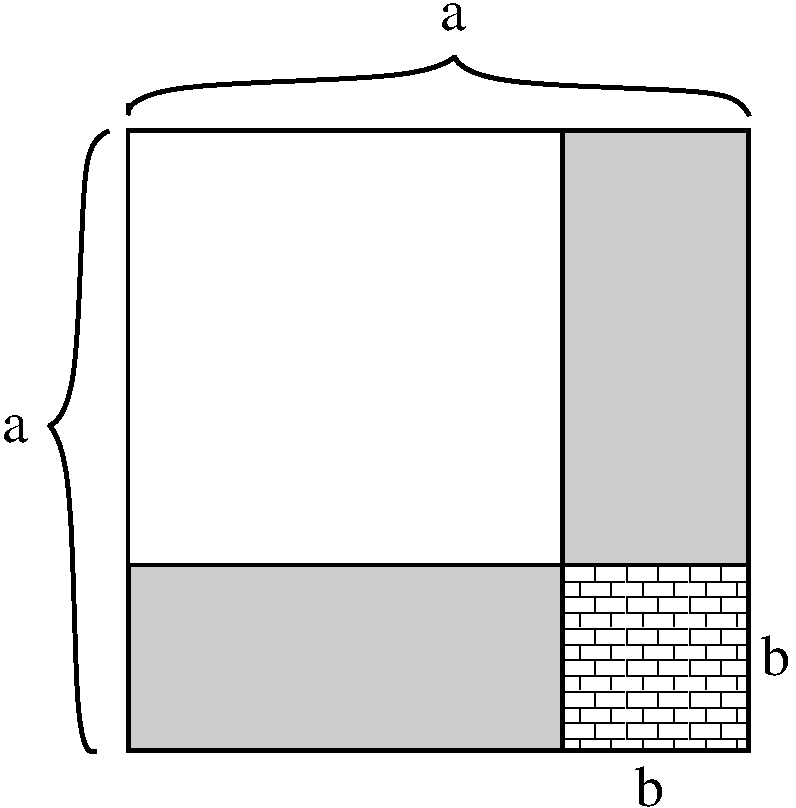
\includegraphics[height=3cm]{img/binF2.pdf}
\end{center}
Gesucht ist der Flächeninhalt des wei\ss en Quadrats: $(a-b)^2$. Das gesamte Quadrat in der Abbildung hat eine Fläche von $ a^2 $. Zur Berechnung stehen zwei weitere Flächen zur Verfügung: Das gekachelte Quadrat besitzt alleine einen Flächeninhalt von $b^2$ und zusammen mit einem grauen Rechteck jeweils einen Flächeninhalt von $ ab $. Um die gesuchte Fläche zu erhalten, können von dem gesamten Quadrat zunächst die zwei grauen Rechtecke entfernt werden, indem $ 2\cdot ab $ abgezogen werden (also: $ -2\cdot ab $). Dadurch wird das gekachelte Quadrat jedoch ein mal zuviel entfernt, so dass es wieder hinzuaddiert werden muss ($+b^2$). Daraus ergibt sich folgende Legende:
\begin{center}
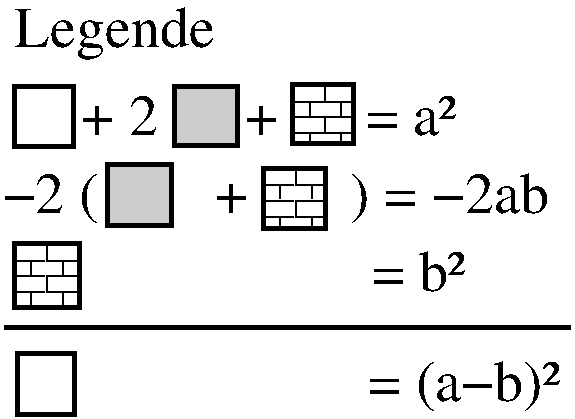
\includegraphics[height=2cm]{img/binF2legende.pdf}
\end{center}
%%%%%%%%%%%%%%%%%%%%%%%%%%%%%%%%%%%%%%%%%%%%%%%%%%%%%%%%%%%%%%
%%%3. Binomische Formeln
%%%%%%%%%%%%%%%%%%%%%%%%%%%%%%%%%%%%%%%%%%%%%%%%%%%%%%%%%%%%%%
\subsubsection{Dritte binomische Formel}
	\[(a + b)(a - b) = a^2 - b^2\]
Die dritte binomische Formel kann mit Hilfe der beiden folgenden Bilder erklärt werden:
\begin{center}
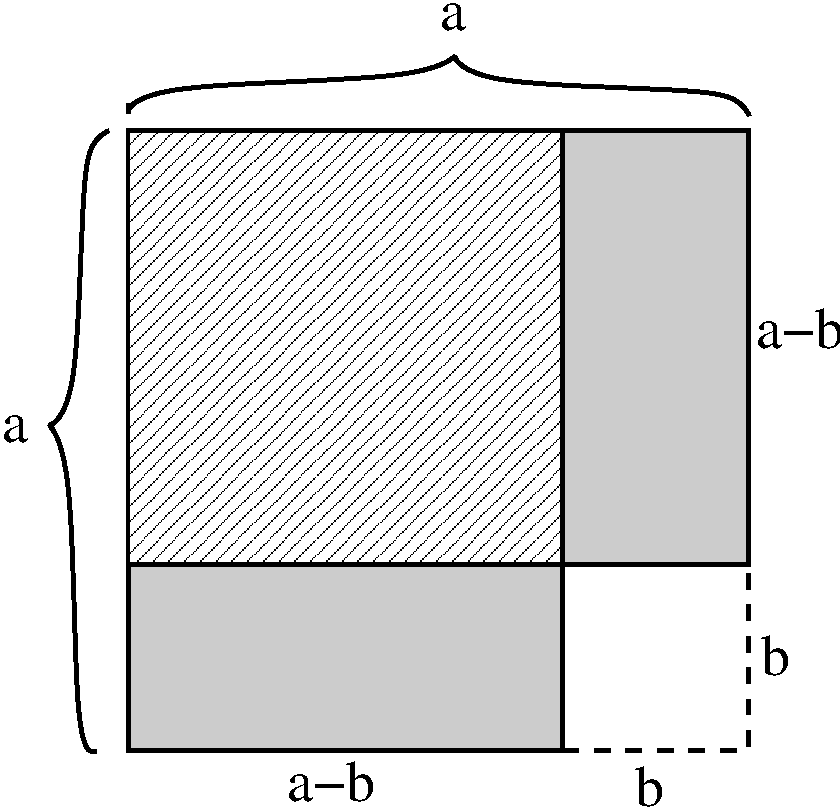
\includegraphics[height=3cm]{img/binF3a.pdf}
\end{center}
Gesucht ist die Fläche, die aus dem schraffierten Quadrat und den beiden grauen Rechtecken besteht. Am einfachsten erhalten wir diese, indem wir (wieder) vom gesamten Quadrat (Fläche: $a^2$) das kleine wei\ss e Quadrat (Fläche: $b^2$) abziehen. Allerdings können wir die Flächen auch so anordnen, dass das folgende Bild entsteht.
\begin{center}
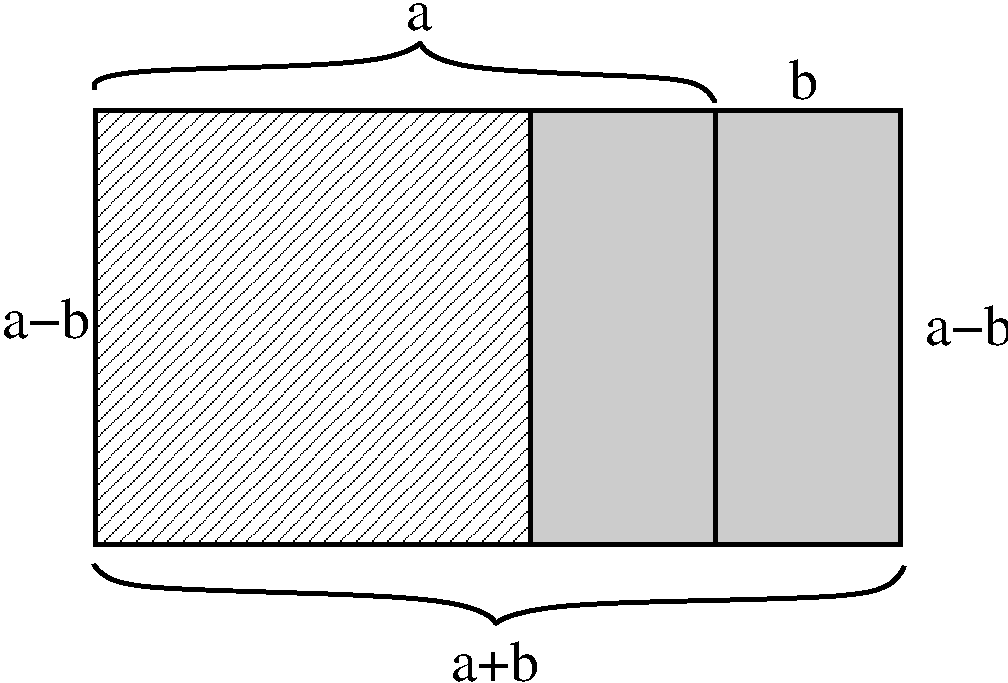
\includegraphics[height=3cm]{img/binF3b.pdf}
\end{center}
Die Fläche eines Rechtecks entspricht dem Produkt seiner Seitenlängen, hier $(a+b)$ und $(a-b)$. Daraus ergibt sich folgende Legende:
\begin{center}
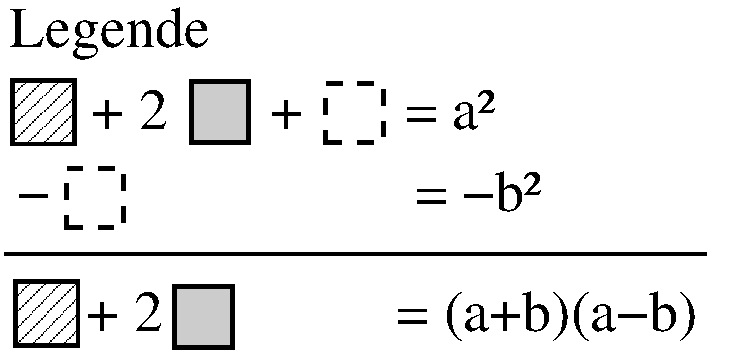
\includegraphics[height=2cm]{img/binF3legende.pdf}
\end{center}
%%%%%%%%%%%%%%%%%%%%%%%%%%%%%%%%%%%%%%%%%%%%%%%%%%%%%%%%%%%%%%
%%%Literatur
%%%%%%%%%%%%%%%%%%%%%%%%%%%%%%%%%%%%%%%%%%%%%%%%%%%%%%%%%%%%%%
\subsection{Literatur}
\begin{itemize}
	\item http://de.wikipedia.org/wiki/Binomische\_Formeln
	\item Formeln und Tabellen für die Sekudarstufen I und II. 7. Aufl. - Berlin: Paetec, Ges. für Bildung und Technik, 1999
\end{itemize}
%%%%%%%%%%%%%%%%%%%%%%%%%%%%%%%%%%%%%%%%%%%%%%%%%%%%%%%%%%%%%%
%%%Aufgaben
%%%%%%%%%%%%%%%%%%%%%%%%%%%%%%%%%%%%%%%%%%%%%%%%%%%%%%%%%%%%%%
\subsection{Aufgaben}

\subsubsection{Aufgabe 1}
Wende die binomischen Formeln zur Vereinfachung an.
\begin{enumerate}
\begin{multicols}{2}
	\item \quad $ (4x + 3y^3)^2 $
	\item \quad $ -(x^4-2)^2 $
	\item \quad $ (x^2-x^3)(x^2+x^3) $
	\item \quad $ (3x^2+2t)^2 $
	\item \quad $ -\frac{1}{2}(x^2-4)^2 $
	\item \quad $ \left(-\frac{1}{2}(x^2-4)\right)^2 $
	\item \quad $ x^2y^2(x^4+2x^2y+y^2) $
\end{multicols}
\end{enumerate}

\pagebreak
\subsubsection{Aufgabe 2}
Vereinfache. Verwende dabei die binomischen Formeln.
\begin{enumerate}
\begin{multicols}{2}
	\item \quad $ (x-3)^n \cdot (x+3)^n $
	\item \quad $ \frac{(a^2-b^2)^3}{(a-b)^3} $
	\item \quad $ \frac{(4-x^2)^n}{(2-x)^n} $
	\item \quad $ \frac{(c-1)^{n-1}}{(c^2-1)^{n-1}} $
	\item \quad $ \frac{(a^{2n}-b^{2n})^2}{(a^n-b^n)^2} $
	\item \quad $ (a^3 - ab^2)(a+b)^2 $
	\item \quad $ \frac{[(x-y)^2]^k}{(x^2-y^2)^k} $
	\item \quad $ (a+b)^4(a-b)^4(a^2-b^2)^5 $
\end{multicols}
\end{enumerate}

\subsubsection{Aufgabe 3}
Faktorisiere/Schreibe als Produkt.
\begin{enumerate}
\begin{multicols}{2}
	\item \quad $ (3x-6)\left(\frac{1}{4}x^2 - x + 1\right) $
	\item \quad $ a^2 - 2a^3 + a^4 $
	\item \quad $ 3a^3 - 12a^9 $
	\item \quad $ x^4 - a^2 $
	\item \quad $ 3-x^2 $
	\item \quad $ x^{2n} + 4x^n + 4 $
	\item \quad $ x^{n+2} -6x^{n+1} + 9x^n $
	\item \quad $ e^{2x}-1 $
	\item \quad $ x^2e^x + 2xe^x +e^x $
\end{multicols}
\end{enumerate}

\subsubsection{Aufgabe 4}
Vereinfache.
\begin{enumerate}
\begin{multicols}{2}
	\item \quad $ \frac{a^3+2a^2b+ab^2}{(a+b)^2} $
	\item \quad $ \frac{a^4-a^2b^2}{ab-a^2} $
	\item \quad $ \frac{t^3+6t^2+9t}{t^2-9} $
	\item \quad $ \frac{x^{2n}-10x^n+25}{x^{2n}-25} $
	\item \quad $ \frac{x^6-t^2}{x^4+tx} $
	\item \quad $ \frac{x^{n+3}-x^{n+1}}{x^{n+1}+x^n} $
	\item \quad $ \frac{(x^2+8xy+16y^2)}{(2x-3y)^{-2}} : \frac{x^2-16y^2}{2x-3y} $
	\item \quad $ \frac{4t^2-4}{t^2+2t+1} $
	\item \quad $ \frac{x^{n-1}-x^n}{x^n-x^{n+2}} $
	\item \quad $ \frac{2(a^2+b^2)^2}{a^5-ab^4} $
	\item \quad $ \frac{x^4-x^3}{x^4-x^2} $
	\item \quad $ \frac{x^3y-xy^5}{x^3y^2-x^2y^4} $
	\item \quad $ \frac{am-an+bm-bn}{a^2-b^2} $
\end{multicols}
\end{enumerate}

\pagebreak
\subsubsection{Aufgabe 5}
Multipliziere aus und vereinfache.
\begin{enumerate}
\begin{multicols}{2}
	\item \quad $ (e^x+e^{-x})^2 $
	\item \quad $ (a^2-a^{-2})^2 $
	\item \quad $ (x^{-2}-3x)(x^{-2}+3x) $
	\item \quad $ (2^{-x}+2^x)(2^{-x}-2^x) $
\end{multicols}
\end{enumerate}

\subsection{Aufgabe 6}
Vereinfache/Fasse zusammen.
\begin{enumerate}
\begin{multicols}{2}
	\item \quad $ \frac{e^{2x}-e^{-2x}}{e^x-e^{-x}} $
	\item \quad $ \left(\frac{x-y}{a-b}\right)^5 \cdot \left(\frac{x-y}{5}\right)^{-2} \cdot \frac{(a-b)^2}{(x^2-y^2)} $
\end{multicols}
\end{enumerate}




\addtocontents{toc}{\setcounter{tocdepth}{0}}
\polyset{style=C, div=:}
\newcommand{\grad}{\ensuremath{\text{grad}\,}}
\newcommand{\halb}{\tfrac{1}{2}}
\section{Polynomdivision}

	Autor: Gerhard Gossen
	
\noindent	\"Uberarbeitung: Marko Rak
	
	\subsection{Polynome}
	
		Ein Polynom ist ein Term der Form
		\[a_nx^n + a_{n-1}x^{n-1} + \dots + a_2x^2 + a_1x + a_0 \quad a_n \neq 0\]
		wobei die $a_i \in \mathbb{R}$, $n \in \mathbb{N}$ und $x$ variabel sind.
		
		Der Grad eines Polynoms ($\grad p(x)$) ist der höchste Exponent von
		$x$. Beispielsweise ist $\grad(3x^2+2x^5-25x) = 5$.
		
	\subsection{Verfahren}
		
		Gegeben sind zwei Polynome $p(x)$ und $q(x)$. Die Division
		$p(x) : q(x)$ ergibt zwei neue Polynome:
		\[p(x) : q(x) = s(x) + \frac{r(x)}{q(x)}.\]
		Dabei ist $r(x)$ der \glqq Rest\grqq{} der Division.
		
		Bei der Berechnung entfernt man die höchsten Terme nacheinander. Dazu sucht
		man einen Term $s_k = b_kx^k$, der mit dem ersten Term von $q$ multipliziert
		den ersten Term von $p$ ergibt. Diesen Term multipliziert man mit $q$ und
		subtrahiert ihn von $p$. Der entstehende Term $p'$ ist vom Grad kleiner als
		$p$. $s_k$ wird zum ersten Term von $s(x)$ (dem \glqq Ergebnispolynom\grqq).
		Dieses Verfahren führt man solange durch wie möglich, also solange
		$\grad p'(x) \geq \grad q(x)$.
		
		\subsection{Beispiel}
			Berechnet werden soll $(-3-3x^2+x+x^3):(1+x)$.
			
			Zuerst ordnen wir die Polynome nach Exponenten: $(x^3-3x^2+x-3):(x+1)$. Im
			ersten Schritt wird also $x^3$ entfernt, der erste Ergebnisterm ist damit
			$x^2$, da $x^2\cdot x = x^3$. Damit subtrahieren wir $x^2(x+1) = x^3+x^2$. 
			
			\polylongdiv[stage=4]{x^3-3x^2+x-3}{x+1}
			
			Jetzt müssen wir also nur noch $(-4x^2+x-3):(x+1)$ berechnen. Wir rechnen
			analog solange wie möglich weiter.
			
			\polylongdiv[stage=10]{x^3-3x^2+x-3}{x+1}
			
			Wir berechnen jetzt $-8:(x+1)$. Da $\grad(-8) < \grad(x+1)$, bricht die
			Polynomdivision hier ab. $-8$ ist der \glqq Rest\grqq{} $r(x)$ der Berechnung.
			
			\polylongdiv{x^3-3x^2+x-3}{x+1}
			
			Das Ergebnis von $(x^3-3x^2+x-3):(x+1)$ ist damit $x^2-4x+5+\frac{-8}{x+1}$.
			Als Probe multiplizieren wir das Ergebnis mit $(x+1)$.
			\begin{align*}\hspace{-11pt}
				(x^2-4x+5+\frac{-8}{x+1})(x+1) 
				&= x^2(x+1)-4x(x+1)+5(x+1)+\frac{-8}{x+1}(x+1)\\
				&= (x^3 + x^2) + (-4x^2 -4x) + (5x +5) + (-8)\\
				&= x^3 -3x^2 +x -3
			\end{align*}
			Dies ist unser ursprüngliches Polynom, wir haben also richtig gerechnet.
		
	\subsection{Weitere Beispiele}
	
		\polylongdiv{4x^5-x^4+2x^3+x^2-1}{x^2+1}
		
		\polylongdiv{x^4 + 2x^3 - 3x^2 - 8x - 4}{x^2 - 4}
		
	\subsection{Aufgaben}
	
		Berechne:
		\begin{enumerate}
			\item $(x^3+1):(x+1)$
			\item $(x^4-x+1):(x^2+x+1)$
			\item $(x^2-9):(x+3)$
			\item $(6x^3-5x^2-36x+35):(3x-7)$
			\item $(x^5-x^2-2x+1) : (x^4-x^3+2x^2-3x+1)$
			\item $(x^5-x^3+x^2+x-2) : (x^2-1)$
			\item $(3x^3+2x^2+4x+9) : (3x+5)$
			\item $(2x^5 + 8x^4 +x^3-x^2 + 12 x +3): (x^2+4x+1)$
			\item $(x^6-2x^5+9x^4-8x^3+15x^2):(x^2-x+5)$
			\item $(2x^7 - x^6 + 3x^5 - \tfrac{1}{2}x^4 + x^3) : (2x^3 - x^2 + 2x)$
			\item $(x^7-6x^5+x^4-11x^2-3x+1):(x^3+2)$
			\item $(3x^5 +6x^4 +\tfrac{11}{3}x^3 + 4x^2 + \tfrac{20}{3}x):(3x^4 +x^3+4x)$
			\item $(\tfrac{1}{6}x^4 + \tfrac{11}{36}x^3 - \tfrac{23}{18}x^2 -
			\tfrac{1}{3}x + \tfrac{2}{3}) : (\tfrac{1}{2}x^2 - \tfrac{4}{3}x +
			\tfrac{2}{3})$
			\item $(\tfrac{5}{4}x^4- \tfrac{1}{4}x^2  + \halb x^5 + \halb x^3 -\halb x)
			: (\halb x^2 +x)$
			\item $(\halb x^5 - \tfrac{3}{4}x^4 - \tfrac{1}{4}x^3 + \tfrac{3}{4}x^2 -
			\tfrac{15}{4}x + \tfrac{7}{4}) : (\halb x -\tfrac{1}{4})$
		\end{enumerate}
		
	\subsection{Literatur}
	
		Beispiele erstellt mit dem \LaTeX-Paket \glq polynom\grq{} von Donald
		Arseneau (\url{http://www.atscire.de/index.php?nav=products/polynom}).
		
		Website mit kommentierter Rechnung und Aufgaben zum Selberrechnen:
		\url{http://www.arndt-bruenner.de/mathe/scripts/polynomdivision.htm}.

\chapter{Quadratische Gleichungen}
	
	Autor: Marc Mittner
	
\noindent	\"Uberarbeitung: Marko Rak, Julia Hempel, Johannes Jendersie
	
	\section{Definition}
		
		Eine quadratische Gleichung ist eine Gleichung, die sich auf die Form 
		\[ ax^2 +bx+c=0 \]
		überführen lässt, mit  $ a, b, c \in \mathbb{R} $.
		
		Eine quadratische Gleichung ist in Normalform, falls $a = 1 $, also
        \begin{align*}
          x^2 &+ px + q=0 \quad\text{mit}\\
          p &= \frac b a \quad\text{und}\\
          q &= \frac c a
        \end{align*}
      
		
	\section{Lösen quadratischer Gleichungen}
		
		Jede quadratische Gleichung hat entweder keine, eine oder zwei reelle Lösungen.
	
		\subsection{Satz von Vieta:}
		Die reellen Zahlen $ a $ und $ b $ sind genau dann Lösungen der Gleichung 
		$x^2 + px + q = 0$, wenn für die Koeffizienten $ p $ und $ q $ gilt:
        \begin{align*}
            p &= -( a + b) \\
            q &= a \cdot b
        \end{align*}
		Daraus folgt:
		Hat eine quadratische Gleichung die Lösungen a und b, so lässt sie sich folgendermaßen darstellen:
		\[ (x - a)(x - b) = 0 \]
		Umgekehrt können die Lösungen aus dieser faktorisierten Form direkt abgelesen werden.
	
		\subsection{Mitternachtsformel}
			
			Jede quadratische Gleichung ($ ax^2 + bx + c = 0 $) kann mit Hilfe der Mitternachtsformel gelöst werden:
			
			\[x_{1,2} = \frac{-b \pm \sqrt{b^2 - 4ac}} {2a}\]
			
		\subsection{p-q-Formel}
			
			Jede quadratische Gleichung in Normalform ($ x^2 + px + q = 0 $) kann mit Hilfe der hergeleiteten p-q-Formel gelöst werden. Die Herleitung erfolgt mit der quadratischen Ergänzung:
			\[ x^2 + px + q = 0\]\\
			\[ x^2 + px + \left({}\frac{p}{2}\right)^2 - \left({}\frac{p}{2}\right)^2 + q = 0\]\\
			\[ \left({}x + \frac{p}{2} \right)^2 = \left({}\frac{p}{2}\right)^2 - q\]\\			
			\[ x_{1,2} = - \frac p 2 \pm \sqrt{\left(\frac p 2 \right)^2 - q} \]\\
			Zusammenhang mit der Mitternachtsformel:
            \begin{align*}
              p &= \frac b a\\
              q &= \frac c a
            \end{align*}

		\subsection{Satz vom Nullprodukt}
			
			Ein Produkt ist genau dann gleich Null, wenn einer seiner Faktoren gleich Null ist. 
			Lässt sich eine Gleichung auf die Form $(ax^2 + bx + c) \cdot x^k = 0$ bringen, so hat die Gleichung nach dem Satz vom Nullprodukt die Lösungen 			$x_{1,2,..,k} = 0$ und die Lösungen $x_{k+1}$ und $x_{k+2}$ können mit Hilfe der Mitternachtsformel / p-q-Formel gelöst werden. 
			
		\subsection{Substitution}
		
		Hat eine Gleichung die Form $ax^{2k} + bx^k + c = 0$, so kann $x^k$ durch eine Variable $u$ substituiert werden: 
		\[au^2 + bu + c = 0 \]
		Diese Gleichung kann dann als quadratische Gleichung gelöst werden. Für die Ergebnisse $ u_1 $ und $ u_2 $ gilt dann:
  \begin{align*}      
u_1 & = x^k& u_2 &= x^k \\
x_{1,2} &= \sqrt[k] {u_1} & x_{3,4} &= \sqrt[k] {u_2}
  \end{align*}

		Dabei gilt für die Anzahl der Lösungen:
		\begin{itemize}
			\item keine Lösung, wenn $ u < 0 $ und $k$ gerade
			\item eine Lösung, wenn $ -\infty < u < \infty $ und $k$ ungerade oder $ u = 0 $ und $k$ gerade.
			\item zwei Lösungen, wenn $ u > 0 $ und $k$ gerade
		\end{itemize}
		
	\section{Beispiele}
\begin{enumerate}
    \item $3x^2  + 3x - 36 = 0$
        
        Ausklammern: \newline
        $\begin{array}{crcl}
            &3(x^2 + x - 12) &=& 0 \\
            &x^2 + x - 12 &=& 0 \\
        \end{array}$ \newline\newline
        Lösen mit p-q-Formel ( $ p = 1 $ , $ q = -12 $ ):\newline
        $\begin{array}{crcl}
         &x_{1,2} &=& - \frac 1 2 \pm \sqrt{\left(\frac 1 2 \right)^2 + 12} \\
        &&=& - \frac 1 2 \pm \sqrt {\frac {49} 4}  \\
        &&=& - \frac 1 2 \pm \frac 7 2 \\
        &x_1 &=& 3 \\
        &x_2 &=& -4 \\
        \end{array}$ \newline\newline
        faktorisierte Darstellung: \newline
        $\begin{array}{crcl}
         &3 (x - 3) (x + 4) &=& 0\\
        \end{array}$
\end{enumerate}

\begin{itemize}        
    \item[2.] $x^7 + 19x^4 - 216x = 0 $\newline\newline
        Ausklammern:\newline
		$\begin{array}{crcl}
			&x(x^6+19x^3-216)&=&0\\
			&x_1&=&0
		\end{array}$           \newline  \newline   
        Substitution von \textit{$ x^3 = u $}: \newline
        $\begin{array}{crcl}
         &u^2 + 19u - 216 &=& 0 \\
        \end{array}$                \newline \newline
        Lösen mit p-q-Formel ($ p = 19 $ , $ q = -216 $): \newline 
        $\begin{array}{crcl}
         &u_{1,2} &=& - \frac {19} 2 \pm \sqrt{\left(\frac {19} 2 \right)^2 + 216} \\
         &&=& - \frac {19} 2 \pm \sqrt{\frac {361} 4 + \frac {864} 4}\\
         &&=& - \frac {19} 2 \pm \sqrt{\frac {1225} 4} \\
         &&=& - \frac {19} 2 \pm \frac {35} 2 \\
        &u_1 &=& 8 \\
        &u_2 &=& -27\\
        \end{array}$   \newline   \newline
        Resubstitution: \newline
        $\begin{array}{ll}
        &x^3 = u_1 \text{\ ergibt die Lösungen}\\
        &x^3 = 8 \\
        &x_2 = 2 \\[2ex]
        &x^3 = u_2 \text{\ ergibt die Lösungen}\\
        &x^3 = -27 \\
        &x_3 = -3\\
        \end{array}$
    
\end{itemize}

		
\section{Aufgaben}
\newcommand{\lineup}{\vspace{-1em}}
	
	%Autor: Marc Mittner
	%\"Uberarbeitung: Marko Rak
	
	Für alle Aufgaben gilt grundsätzlich:
	$ x, y, z \in \mathbb{R} $ sind Variable
	$ a, b, c \in \mathbb{R} $ sind feste Parameter
	
	Lösen Sie die folgenden Gleichungen:
	\begin{enumerate}\abovedisplayskip-1em
		\item 
		\[ x^2 - x - 2 = 0 \]
		\item
		\[4x^2 + 16x - 84 = 0 \]
		\item
		\[\frac 1 2 x^2 + 3x + 4 = 0 \]
		\item
		\[4x^2 + 48x + 144 = 0 \]
		\item 
		\[(x - \sqrt{157})^2 = 0 \]
		\item
		\[\frac 7 3 x^3 + \frac {49} 3 x^2 + 35x + 21 = 0 \]
		\item
		\[\frac 7 4 x^2 + 7x = -7 \]
		\item
		\[ |x^2| = 4 \]
		\item
		\[ |x|^2 = 4 \]
		\item
		\[ |x^2 - 4 | = 2 \]
		\item
		\[x^2 = x + 12 \]
		\item
		\[3x^2 + 4x + 1 = 0\]
		\item
		\[x^5 - 25x^3 + 144x = 0 \]
		\item
		\[(x - \pi)(x + \pi) = 0 \]
		\item
		\[\frac {x^3 - 2x^2} {x - 2} + \frac {2x^2 + 4x} {x + 2} = \-1\]
		\item
		\[x^4 - 14x^3 + 59x^2 - 70x = 0\]
		\item
		\[3x^7 - 42x^5 + 147x^3 = 0\]
		\item
		\[x^{12} = 4096\]
		\item
		\[x^4 + 4x^3 + 6x^2 + 4x + 1 = 0\]
		\item
		\[(\sqrt 2 x + 2 \sqrt 2)^2 = 0\]
		\item
		\[2ax^2 - 12ax + 18a = 0\]
		\item
		\[\frac 1 {x^2} + 1 = 2\]
		\item
		\[\frac 4 x + x = 4\]
	\end{enumerate}
\addtocontents{toc}{\setcounter{tocdepth}{1}}
\chapter{Lineare Gleichungssysteme}
	
	Autor: Marko Rak
	
	\section{Definition}
	
		Als \emph{lineares Gleichungssystem} bezeichnet man eine Menge von $m$ Gleichungen,
		die $n$ Unbekannte enthalten.
		Allgemein l\"asst sich solch ein Gleichungssystem immer in folgender Form darstellen:
		\[
			\begin{array} {ccccccccccc}
				a_{11} x_1 & + & a_{12} x_2 & + & a_{13} x_3 & + & \cdots & + & a_{1n} x_n & = & b_1\\
				a_{21} x_1 & + & a_{22} x_2 & + & a_{23} x_3 & + & \cdots & + & a_{2n} x_n & = & b_2\\
				a_{31} x_1 & + & a_{32} x_2 & + & a_{33} x_3 & + & \cdots & + & a_{3n} x_n & = & b_3\\
				\vdots & & & & & & \ddots & & & & \vdots\\
				a_{m1} x_1 & + & a_{m2} x_2 & + & a_{m3} x_3 & + & \cdots & + & a_{mn} x_n & = & b_m\\
			\end{array}
		\]
		
	\section{Lineare Abh\"angigkeit}
		
		Eine lineare Gleichung der obigen Form ist \emph{linear abh\"angig},
		wenn sie sich durch die anderen Gleichungen des Systems und der Multiplikation mit einer Konstanten $c_i$ darstellen l\"asst.
		\[
			\begin{array} {ccccccccccccc}
				& &a_{11} x_1 & + & a_{12} x_2 & + & \cdots & + & a_{1n} x_n & - & b_1 &  & \\
				 & = & (a_{21} x_1 & + & a_{22} x_2 & + & \cdots & + & a_{2n} x_n & - & b_2) & c_2 \\
				& + & (a_{31} x_1 & + & a_{32} x_2 & + & \cdots & + & a_{3n} x_n & - & b_3) & c_3\\
				 &\vdots &  & & & & \ddots  & & & & & \vdots\\
				& + & (a_{m1} x_1 & + & a_{m2} x_2 & + & \cdots & + & a_{mn} x_n & - & b_m) & c_n \\
			\end{array}
		\]
		
		Andernfalls ist sie \emph{linear unabh\"angig} von den anderen Gleichungen des Systems.
		
	\section{L\"osbarkeit}
	
		Ob ein lineares Gleichungssystem l\"osbar ist und wie viele L\"osungen es hat, ist unterschiedlich.
		Dabei tritt immer einer der folgenden F\"alle auf:
		
		\begin{enumerate}
			\item Das Gleichungssystem hat keine L\"osung.
			\item Das Gleichungssystem hat genau eine L\"osung.
			\item Das Gleichungssystem hat mehrere (meist unendlich viele) L\"osungen.
		\end{enumerate}
		
		\noindent Kriterien f\"ur die L\"osbarkeit und die Zuteilung eines linearen Gleichungssystems zu einem dieser F\"alle,
		w\"urde dem Vorlesungsinhalt vorgreifen und wird daher hier nicht ausf\"uhrlich erkl\"art.
		Allgemein l\"asst sich jedoch sagen:
		Hat ein lineares Gleichungssystem mehr Unbekannte als linear unabh\"angige Gleichungen,
		so hat es mehrere L\"osungen.
		
	\section{L\"osungsverfahren}
	
		Neben den bereits bekannten L\"osungsverfahren wie Gleich-, Einsetzungsverfahren usw., existieren noch weitere, systematische Verfahren.
		Dazu z\"ahlt u.A. das \emph{Gauss-Verfahren} (auch \emph{Gauss-Algorithmus} genannt),
		welches unter Verwendung einer vereinfachten Gleichungssystemdarstellung eine Diagonalform oder auch Dreiecksform erstellt.
		Diese beschleunigt das Finden von L\"osungen.
		
		\subsection{Vereinfachte Darstellung}
		
			Ein allgemeines lineares Gleichungssystem
			\[
				\begin{array} {ccccccccccc}
					a_{11} x_1 & + & a_{12} x_2 & + & a_{13} x_3 & + & \cdots & + & a_{1n} x_n & = & b_1\\
					a_{21} x_1 & + & a_{22} x_2 & + & a_{23} x_3 & + & \cdots & + & a_{2n} x_n & = & b_2\\
					a_{31} x_1 & + & a_{32} x_2 & + & a_{33} x_3 & + & \cdots & + & a_{3n} x_n & = & b_3\\
					\vdots & & & & & & \ddots & & & & \vdots\\
					a_{m1} x_1 & + & a_{m2} x_2 & + & a_{m3} x_3 & + & \cdots & + & a_{mn} x_n & = & b_m\\
				\end{array}
			\]
			l\"asst sich vereinfacht wie folgt darstellen:
			\[
				\begin{tabular} {ccccc|c}
					$x_1$ & $x_2$ & $x_3$ & $\cdots$ & $x_n$ &\\
					\hline
					$a_{11}$ & $a_{12}$ & $a_{13}$ & $\cdots$ & $a_{1n}$ & $b_1$\\
					$a_{21}$ & $a_{22}$ & $a_{23}$ & $\cdots$ & $a_{2n}$ & $b_2$\\
					$a_{31}$ & $a_{32}$ & $a_{33}$ & $\cdots$ & $a_{3n}$ & $b_3$\\
					$\vdots$ & & & $\ddots$ & & $\vdots$\\
					$a_{m1}$ & $a_{m2}$ & $a_{m3}$ & $\cdots$ & $a_{mn}$ & $b_m$\\
				\end{tabular}
			\]
			
			\noindent Nun werden die Unbekannten,
			da in allen Gleichungen der Systems gleich,
			nur noch im Tabellenkopf dargestellt.
			Tauchen in Gleichungen des Systems bestimmte Unbekannte nicht auf,
			werden sie in dieser Tabellendarstellung mit Faktor 0 aufgef\"uhrt.
			Das Gleichheitszeichen wird nun repr\"asentiert durch die Trennung vor der letzten Spalte.
			Auf die Additionsoperatoren wird gezielt verzichtet und die Subtraktion wird als Addition mit einem negativen   	Operanden betrachtet.
            Elementare Umformungen \"andern nichts an der L\"osung des linearen Gleichungssystems.
			Unter elementare Umformungen versteht man:

			\begin{enumerate}
				\item das Vertauschen von Spalten oder Zeilen
				\item die Multiplikation einer Zeile mit einer Konstanten
				\item die Addition eines Vielfachen einer Zeile zu einer anderen
			\end{enumerate}
						
		\subsection{Diagonalform}
		
			Die \emph{Diagonalform} des obigen allgemeinen linearen Gleichungssystems sieht wie folgt aus:
			\[
				\begin{tabular} {ccccccc|c}
					$x_1$ & $x_2$ & $x_3$ & $x_4$ & $\cdots$ & $x_{n-1}$ & $x_n$ &\\
					\hline
					$a_{11}$ & $a_{12}$ & $a_{13}$ & $a_{14}$ & $\cdots$ & $a_{1(n-1)}$ & $a_{1n}$ & $b_{1}$\\
					0 & $a_{22}^*$ & $a_{23}^*$ & $a_{24}^*$ & $\cdots$ & $a_{2(n-1)}^*$ & $a_{2n}^*$ & $b_{2}^*$\\
					0 & 0 & $a_{33}^*$ & $a_{34}^*$ & $\cdots$ & $a_{3(n-1)}^*$ & $a_{3n}^*$ & $b_{3}^*$\\
					0 & 0 & 0 & $a_{44}^*$ & $\cdots$ & $a_{4(n-1)}^*$ & $a_{3n}^*$ & $b_{3}^*$\\
					$\vdots$ & & & & $\ddots$ & & & $\vdots$\\
					0 & 0 & 0 & 0 & $\cdots$ & $a_{(m-1)(n-1)}^*$ & $a_{(m-1)n}^*$ & $b_{m-1}^*$\\
					0 & 0 & 0 & 0 & $\cdots$ & 0 & $a_{mn}^*$ & $b_{m}^*$\\
				\end{tabular}
			\]
			
			\noindent Mittels dieses Schemas lassen sich die L\"osungen des linearen Gleichungssystem relativ leicht erschlie\ss en.
			Man beginnt von unten und arbeitet sich zeilenweise aufw\"arts.
			Dabei kann mit jeder neuen Zeile eine weitere Unbekannte bestimmt werden.
			
			\noindent Aus der letzten Zeile
			\[
				a_{mn}^* x_n = b_{m}^*
			\]
			ergibt sich
			\[
				x_n = \frac {b_m^*} {a_{mn}^*}.
			\]
			Nun wird $x_n$ in die vorletzte Zeile
			\[
				a_{(m-1)(n-1)}^* x_{n-1} + a_{(m-1)n}^* x_n = b_{m-1}^*
			\]
			eingesetzt und nach $x_{n-1}$ umgestellt, was
            \[
				x_{n-1} = \frac {b_{m-1}^* -  \frac {a_{(m-1)n}^*} {a_{mn}^*} b_m^*} {a_{(m-1)(n-1)}^*}
			\]
			
			\noindent ergibt.
			Dies wird zeilenweise aufsteigend bis zur ersten Gleichung fortgesetzt,
			sodass gegebenenfalls alle Unbekannten ermittelt werden k\"onnen.
			
		\subsection{Gauss-Algorithmus}
		
			Der bereits angesprochende \emph{Gauss-Algorithmus} dient der Herstellung der Diagonalform aus einem beliebigen linearen Gleichungssystem.
			Dazu wird die vereinfachte Darstellung genutzt und mittels elementarer Umformungen schrittweise die Dreiecksform erstellt.
			Wir w\"ahlen in jedem Schritt eine Gleichung
			und addieren ein Vielfaches dieser zu jeder anderen Gleichung,
			um eine Spalte mit m\"oglichst vielen Nullen zu erzeugen.
			
			
			\noindent Die Ausgangssituation stellt sich wie folgt dar:
			
			\[
				\begin{tabular} {ccccc|c}
					$x_1$ & $x_2$ & $x_3$ & $\cdots$ & $x_n$ &\\
					\hline
					$a_{11}$ & $a_{12}$ & $a_{13}$ & $\cdots$ & $a_{1n}$ & $b_1$\\
					$a_{21}$ & $a_{22}$ & $a_{23}$ & $\cdots$ & $a_{2n}$ & $b_2$\\
					$a_{31}$ & $a_{32}$ & $a_{33}$ & $\cdots$ & $a_{3n}$ & $b_3$\\
					$\vdots$ & & & $\ddots$ & & $\vdots$\\
					$a_{m1}$ & $a_{m2}$ & $a_{m3}$ & $\cdots$ & $a_{mn}$ & $b_m$\\
				\end{tabular}
			\]
			
			\noindent Wir w\"ahlen die erste Gleichung aus und addieren ein Vielfaches davon zu den anderen Gleichungen,
			um in der ersten Spalte Nullen zu erzeugen.
			
			\[
				\begin{array} {ccccc|ccccc}
					x_1 & x_2 & x_3 & \cdots & x_n & & & & & \\
					\hline
					a_{11} & a_{12} & a_{13} & \cdots & a_{1n} & b_1 & \cdot(-\frac {a_{21}} {a_{11}}) & \cdot(-\frac {a_{31}} {a_{11}}) & \cdots & \cdot(-\frac {a_{m1}} {a_{11}})\\
					a_{21} & a_{22} & a_{23} & \cdots & a_{2n} & b_2 & \hookleftarrow & & &  \\
					a_{31} & a_{32} & a_{33} & \cdots & a_{3n} & b_3 & & \hookleftarrow & &  \\
					\vdots & & & \ddots & & \vdots & & & \ddots & \\
					a_{m1} & a_{m2} & a_{m3} & \cdots & a_{mn} & b_m & & & & \hookleftarrow  \\
				\end{array}
			\]
			
			\noindent Somit ergibt sich nach dem ersten Schritt diese Tabelle:
			
			\[
				\begin{tabular} {ccccc|c}
					$x_1$ & $x_2$ & $x_3$ & $\cdots$ & $x_n$ &\\
					\hline
					$a_{11}$ & $a_{12}$ & $a_{13}$ & $\cdots$ & $a_{1n}$ & $b_1$\\
					0 & $a_{22}'$ & $a_{23}'$ & $\cdots$ & $a_{2n}'$ & $b_2'$\\
					0 & $a_{32}'$ & $a_{33}'$ & $\cdots$ & $a_{3n}'$ & $b_3'$\\
					$\vdots$ & & & $\ddots$ & & $\vdots$\\
					0 & $a_{m2}'$ & $a_{m3}'$ & $\cdots$ & $a_{mn}'$ & $b_m'$\\
				\end{tabular}
			\]
			
			\noindent Nun w\"ahlen wir die zweite Gleichung und addieren ein Vielfaches davon zu jeder folgenden Gleichung,
			um in der zweiten Spalte auch Nullen zu erzeugen.
			
			\[
				\begin{tabular} {ccccc|cccc}
					$x_1$ & $x_2$ & $x_3$ & $\cdots$ & $x_n$ & & & & \\
					\hline
					$a_{11}$ & $a_{12}$ & $a_{13}$ & $\cdots$ & $a_{1n}$ & $b_1$ & & \\
					0 & $a_{22}'$ & $a_{23}'$ & $\cdots$ & $a_{2n}'$ & $b_2'$ & $\cdot (-\frac {a_{32}'}{a_{22}'})$ & $\cdots$ & $\cdot (-\frac {a_{m2}'}{a_{22}'})$\\
					0 & $a_{32}'$ & $a_{33}'$ & $\cdots$ & $a_{3n}'$ & $b_3'$ & $\hookleftarrow$ & & \\
					$\vdots$ & & & $\ddots$ & & $\vdots$ & & $\ddots$ & \\
					0 & $a_{m2}'$ & $a_{m3}'$ & $\cdots$ & $a_{mn}'$ & $b_m'$ & & & $\hookleftarrow$  \\
				\end{tabular}
			\]
			
			\noindent Was uns nach dem zweiten Schritt zu der folgenden Tabelle bringt:
			
			\[
				\begin{tabular} {ccccc|c}
					$x_1$ & $x_2$ & $x_3$ & $\cdots$ & $x_n$ &\\
					\hline
					$a_{11}$ & $a_{12}$ & $a_{13}$ & $\cdots$ & $a_{1n}$ & $b_1$\\
					0 & $a_{22}'$ & $a_{23}'$ & $\cdots$ & $a_{2n}'$ & $b_2'$\\
					0 & 0 & $a_{33}''$ & $\cdots$ & $a_{3n}''$ & $b_3''$\\
					$\vdots$ & & & $\ddots$ & & $\vdots$\\
					0 & 0 & $a_{m3}''$ & $\cdots$ & $a_{mn}''$ & $b_m''$\\
				\end{tabular}
			\]
			
			\noindent Dieser Ablauf wird wiederholt, bis die gew\"unschte Diagonalform entstanden ist
			und sich das erzeugte Schema wie oben beschrieben aufl\"osen l\"asst.
			
			\[
				\begin{tabular} {cccccc|c}
					$x_1$ & $x_2$ & $x_3$ & $\cdots$ & $x_{n-1}$ & $x_n$ &\\
					\hline
					$a_{11}$ & $a_{12}$ & $a_{13}$ & $\cdots$ & $a_{1(n-1)}$ & $a_{1n}$ & $b_{1}$\\
					0 & $a_{22}^*$ & $a_{23}^*$ & $\cdots$ & $a_{2(n-1)}^*$ & $a_{2n}^*$ & $b_{2}^*$\\
					0 & 0 & $a_{33}^*$ & $\cdots$ & $a_{3(n-1)}^*$ & $a_{3n}^*$ & $b_{3}^*$\\
					$\vdots$ & & & $\ddots$ & & & $\vdots$\\
					0 & 0 & 0 & $\cdots$ & 0 & $a_{mn}^*$ & $b_{m}^*$\\
				\end{tabular}
			\]
				
	\section{Beispiele}
	
		F\"ur alle Beispiele gilt $ x_i \in \mathbb{R} $ 
		
		\begin{enumerate}
				\item
				
					Die Ausgangssituation stellt sich wie folgt dar:
					\[
						\begin{array} {ccccccc}
							3 x_1 & - & 1 x_2 & + & 2 x_3 & = & 1\\
							7 x_1 & - & 4 x_2 & - & 1 x_3 & = & -2\\
							- x_1 & - & 3 x_2 & - & 12 x_3 & = & -5\\
						\end{array}
					\]
					
					und l\"asst sich vereinfacht darstellen:
					\[
						\begin{tabular} {ccc|c}
							$x_1$ & $x_2$ & $x_3$ &\\
							\hline
							3 & -1 & 2 & 1\\
							7 & -4 & -1 & -2\\
							-1 & -3 & -12 & -5\\
						\end{tabular}
					\]
					
					Jetzt wird schrittweise die Diagonalform erzeugt.
					Um Zeit und Platz zu sparen, lassen sich alle Schritte in einer Tabelle durchf\"uhren.
					\[
						\begin{tabular} {ccc|ccc}
							$x_1$ & $x_2$ & $x_3$ & & &\\
							\hline
							3 & -1 & 2 & 1 & $\cdot (-\frac{7} {3})$ & $\cdot (\frac{1} {3})$\\
							7 & -4 & -1 & -2 & $\hookleftarrow$ &\\
							-1 & -3 & -12 & -5 & & $\hookleftarrow$\\
							\hline
							3 & -1 & 2 & 1 & &\\
							0 & $-\frac{5} {3}$ & $-\frac{17} {3}$ & $-\frac{13} {3}$ & $\cdot (-2)$ &\\
							0 & $-\frac{10} {3}$ & $-\frac{34} {3}$ & $-\frac{14} {3}$ & $\hookleftarrow$ &\\
							\hline
							3 & -1 & 2 & 1 & &\\
							0 & $-\frac{5} {3}$ & $-\frac{17} {3}$ & $-\frac{13} {3}$ & &\\
							0 & 0 & 0 & 4 & &\\
						\end{tabular}
					\]
					
					Nach Herstellung der Diagonalform l\"asst sich das Ergebnis wie oben beschrieben leicht erschlie\ss en.
					In diesem Beispiel entsteht ein Widerspruch in der letzten Gleichung
					\[
						0 x_1 + 0 x_2 + 0 x_3 = 4.
					\]
					
					Somit hat das lineare Gleichungssystem keine L\"osung.
					
				\item
				
					Eine weitere, diesmal gleich vereinfachte, Aufgabenstellung.
					\[
						\begin{tabular} {ccc|c}
							$x_1$ & $x_2$ & $x_3$ &\\
							\hline
							2 & -5 & 3 & 3\\
							4 & -12 & 8 & 4\\
							3 & 1 & -2 & 9\\
						\end{tabular}
					\]
					
					Die schrittweise Umformung:
					\[
						\begin{tabular} {ccc|ccc}
							$x_1$ & $x_2$ & $x_3$ & & &\\
							\hline
							2 & -5 & 3 & 3 & $\cdot (-2)$ & $\cdot (-\frac{3} {2})$\\
							4 & -12 & 8 & 4 & $\hookleftarrow$ &\\
							3 & 1 & -2 & 9 & & $\hookleftarrow$\\
							\hline
							2 & -5 & 3 & 3 & &\\
							0 & -2 & 2 & -2 & $\cdot (\frac{17} {4})$ &\\
							0 & $\frac{17} {2}$ & $-\frac{13} {2}$ & $\frac{9} {2}$ & $\hookleftarrow$ &\\
							\hline
							2 & -5 & 3 & 3 & &\\
							0 & -2 & 2 & -2 & &\\
							0 & 0 & 2 & -4 & &\\
						\end{tabular}
					\]
					
					Es ergibt sich also nacheinander aus den letzten drei Gleichungen.
					\[
						\begin{array} {ccc}
							x_3 & = & -2\\
							x_2 & = & -1\\
							x_1 & = & 2\\
						\end{array}
					\]
					
					Somit hat das lineare Gleichungssystem genau eine L\"osung.

				\item
				
					Ein letztes Beispiel in aller K\"urze.
					\[
						\begin{tabular} {ccc|ccc}
							$x_1$ & $x_2$ & $x_3$ & & &\\
							\hline
							1 & -2 & 3 & 4 & $\cdot (-3)$ & $\cdot (-2)$\\
							3 & 1 & -5 & 5 & $\hookleftarrow$ &\\
							2 & -3 & 4 & 7 & & $\hookleftarrow$\\
							\hline
							1 & -2 & 3 & 4 & &\\
							0 & 7 & -14 & -7 & $\cdot (-\frac{1} {7})$ &\\
							0 & 1 & -2 & -1 & $\hookleftarrow$ &\\
							\hline
							1 & -2 & 3 & 4 & &\\
							0 & 7 & -14 & -7 & &\\
							0 & 0 & 0 & 0 & &\\
						\end{tabular}
					\]
					
					Es ist eine Nullzeile entstanden,
					welche auftritt, wenn zwei Gleichungen linear abh\"angig sind.
					Folglich hat das lineare Gleichungssystem nur noch 2 (linear unabh\"angige) Gleichungen und 3 Unbekannte.
					Es l\"asst sich eine Variable frei w\"ahlen, was zu unendlich vielen L\"osungen f\"ur dieses lineare Gleichungssystems f\"uhrt.
					Wir setzen also
					\[
						x_3 = t, t \in \mathbb{R}
					\]
					
					und l\"osen nun die anderen Unbekannten in Abh\"angigkeit von $t$ auf.
					\[
						\begin{array} {ccccc}
							x_2 & = & -1 & + & 2t\\
							x_1 & = & 2 & + & t\\
						\end{array}
					\]
				
		\end{enumerate}
		
		
	\section{Literatur}
	
 \begin{description}
     \item[Grundstudium.info]  \texttt{http://www.grundstudium.info/\allowbreak linearealgebra/\\\allowbreak lineare\_\allowbreak algebra\_grundlagennode9.php}
     \item[Mathematik.de] \texttt{http://www.mathematik.de/mde/fragenantworten/\\erstehilfe/linearegleichungssysteme/\\linearegleichungssysteme.html}
 \end{description}
   
		
		

		
  %\href{http://www.mathematik.de/mde/fragenantworten/erstehilfe/linearegleichungssysteme/linearegleichungssysteme.html}{http://www.mathematik.de/mde/fragenantworten/\\erstehilfe/linearegleichungssysteme/linearegleichungssysteme.html}
	
	\newpage
	\section{Aufgaben}
	
		F\"ur alle Aufgaben gilt $ x_i \in \mathbb{R} $ und $ a, b \in \mathbb{R} $ sind fest.
		
		\subsection{Einfache Gleichungssysteme}
			Bestimmen Sie die L\"osungen folgender Gleichungssysteme.

			\begin{enumerate}\abovedisplayskip-1em
				\item 
				
					\[
						\begin{array} {ccccccc}
							x_1 & + & 5 x_2 & + & 2 x_3 & = & 3 \\
							2 x_1 & - & 2 x_2 & + & 4 x_3 & = & 5\\
							x_1 & + & x_2 & + & 2 x_3 & = & 1\\
						\end{array}
					\]
				
				\item
				
					\[
						\begin{array} {ccccccc}
							7 x_1 & + & 8 x_2 & + & 5 x_3 & = & 3 \\
							3 x_1 & - & 3 x_2 & + & 2 x_3 & = & 1\\
							18 x_1 & + & 21 x_2 & + & 13 x_3 & = & 8\\
						\end{array}
					\]
				
				\item
					
					\[
						\begin{array} {ccccccccc}
							x_1 & + & x_2 & + & 3 x_3 & + & 4 x_4 & = & -3 \\
							2 x_1 & + & 3 x_2 & + & 11 x_3 & + & 5 x_4 & = & 2\\
							2 x_1 & + & x_2 & + & 3 x_3 & + & 2 x_4 & = & -3\\
							x_1 & + & x_2 & + & 5 x_3 & + & 2 x_4 & = & 1\\
						\end{array}
					\]	
						
				\item
					
					\[
						\begin{array} {ccccccc}
							x_1 & + & 2 x_2 & + & 3 x_3 & = & -4 \\
							5 x_1 & - & x_2 & + & x_3 & = & 0\\
							7 x_1 & + & 3 x_2 & + & 7 x_3 & = & -8\\
							2 x_1 & + & 3 x_2 & - & x_3 & = & 11\\
						\end{array}
					\]
						
				\item
					
					\[
						\begin{array} {cccccccccccc}
							- x_1 & + & x_2 & + & x_3 & & & - & x_5 & = & 0 \\
							x_1 & - & x_2 & - & 3 x_3 & + & 2 x_4 & - & x_5 & = & 2\\
							& & 3 x_2 & - & x_3 & - & 5 x_4 & - & 7 x_5 & = & 9\\
							3 x_1 & - & 3 x_2 & - & 5 x_3 & + & 2 x_4 & + & 5 x_5 & = & 2\\
						\end{array}
					\]	
	
				\item
					
					\[
						\begin{array} {ccccccccc}
							x_1 & - & 2 x_2 & - & 3 x_3 & & & = & -7 \\
							2 x_1 & - & x_2 & + & 2 x_3 & + & 7 x_4 & = & -3\\
							-2 x_1 & + & x_2 & + & 3 x_3 & + & 3 x_4 & = & 8\\
							x_1 & + & 4 x_2 & + & 5 x_3 & - & 2 x_4 & = & 7\\
						\end{array}
						\]
						
				\item
					
					\[
						\begin{array} {ccccccc}
							x_1 & - & x_2 & + & x_3 & = & 4 \\
							x_1 & + & 2 x_2 & + & x_3 & = & 13\\
							4 x_1 & + & 5 x_2 & + & 4 x_3 & = & 43\\
							2 x_1 & + & 4 x_2 & + & 2 x_3 & = & 26\\
						\end{array}
					\]
					

			\end{enumerate}
			
		\subsection{Parametrisierte Gleichungssysteme}
				
			Bestimmen Sie die L\"osungen folgender Gleichungssysteme in Abh\"angigkeit von $a$ und $b$.

			\begin{enumerate}\abovedisplayskip-1em
				\item
				
					\[
						\begin{array} {ccccccc}
							2 x_1 & - & x_2 & + & 4 x_3 & = & 0 \\
							x_1 & + & 3 x_2 & - & x_3 & = & 0\\
							7 x_1 & + & 7 x_2 & + & (4-a) x_3 & = & 0\\
						\end{array}
					\]
						
				\item
					
					\[
						\begin{array} {ccccccc}
							x_1 & + & x_2 & + & x_3 & = & 0 \\
							x_1 & + & a x_2 & + & x_3 & = & 4\\
							a x_1 & + & 3 x_2 & + & a x_3 & = & -2\\
						\end{array}
					\]
					
				\item
					
					\[
						\begin{array} {ccccccc}
							x_1 & - & 2 x_2 & + & 3 x_3 & = & 4 \\
							2 x_1 & + & x_2 & + & x_3 & = & -2\\
							x_1 & + & a x_2 & + & 2 x_3 & = & b\\
						\end{array}
					\]
					
			\end{enumerate}


\chapter{Betrag, Ungleichungen, Kreis}
\section{Betrag}
Autor: Marc Mittner

\noindent "Uberarbeitung: Christian Rutsch

\subsection{Definition}
F"ur eine reelle Zahl $x$ ist der Betrag definiert als: 

%\large
%$ | x | =  \left\{ ^{  x , x \geq 0}_{-x , x < 0} \right. $
$\vert x \vert = \left\{
\begin{array}{ccc}
x, && x \geq 0\\
-x,&&x < 0
\end{array}\right.$
%\normalsize

\subsection{Die Betragfunktion}
Graph der Betragfunktion $ f(x) = |x| $ ist:
\begin{itemize}
\item symmetrisch zur y-Achse 
\item $y \geq 0$ f"ur alle Werte $ x \in \mathbb{R} $.
\end{itemize}

\begin{center}
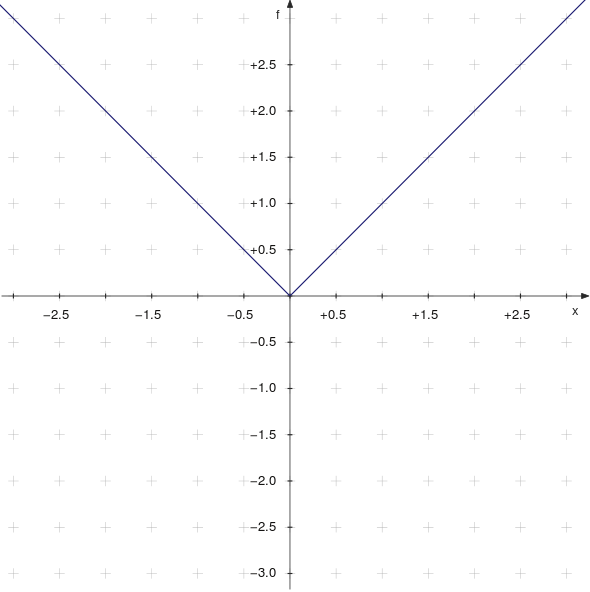
\includegraphics[scale=0.25]{img/betrag/betrag.png}
\end{center}

%\pagebreak
\subsection{Rechenregeln f"ur den Betrag}
\begin{enumerate}
\item $|-a|=|a|$
\item $|a|\geq0; |a|=0\Leftrightarrow a=0$
\item $|a\cdot b|=|a|\cdot |b|$
\item $|\frac{a}{b}|=\frac{|a|}{|b|}$ f"ur b$\neq0$
\item $|a^n|=|a|^n$ f"ur n$\in\mathbb{N}$
\item $|a+b|\leq|a|+|b|$ (sogenannte Dreiecksungleichung)
\end{enumerate}
\subsection{Beispiele}
Gleichungen mit Betr"agen werden durch Fallunterscheidung gel"ost.
\begin{enumerate}
 \item $ | x-1 | = 3 $

Fallunterscheidung

1.Fall:
\begin{align*}
  (x - 1) &= 3 \\
  x &= 4
\end{align*}

2. Fall:
\begin{align*}
-(x - 1) &= 3 \\
 x &= -2
\end{align*}



\item $(x + 3)^2 = 4   \rightarrow | x+3 | = 2$
   
Fallunterscheidung

1. Fall:
\begin{align*}
+(x + 3) &= 2 \\
\rightarrow x &= -1
\end{align*}
2. Fall:
\begin{align*}
-(x + 3) &= 2 \\
\rightarrow -x - 3 &= 2\\
 \rightarrow x &= -5
\end{align*}

\end{enumerate}

\subsection{Aufgaben}
L"osen Sie die folgenden Gleichungen: 
\begin{enumerate}
\item $|x| = 7$
\item $| x+5 | = 10$
\item $| 2x-3 | = 1$
\item $| 2x-4| = 6x+36$
\end{enumerate}

\section{Rund um den Kreis}
Autor: Marc Mittner

\noindent "Uberarbeitung: Christian Rutsch

\subsection{Definition}
Ein Kreis beschreibt die Menge aller Punkte, die von einem gegebenen Mittelpunkt aus den gleichen Abstand haben -- oder als mathematisch saubere Definition:
\[ K = \lbrace X \in E ,\  |\overline {MX}| = r \rbrace \]
(Erl"auterung: Der Kreis $K$ ist eine Menge, die alle Punkte $X$ einer Ebene $E$ enth"alt, f"ur die gilt, dass die L"ange der Strecke $\overline{MX}$ gerade den Radius $r$ ergibt.)

\subsection{Mathematische Beschreibung}
F"ur die mathematische Beschreibung eines Kreises gibt es verschiedene M"oglichkeiten. Hier soll nur die Darstellung mit kartesischen Koordinaten behandelt werden.

\subsection{Koordinatengleichung}
Die Koordinatengleichung eines Kreises im kartesischen Koordinatensystem lautet:
\[ (x - x_M)^2 + (y - y_M)^2 = r^2 \]
Der Mittelpunkt des Kreises ist dabei $M = (x_M , y_M)$, der Radius des Kreises ist $r$.
Durch den Satz des Pythagoras wird klar, wie diese Beziehung zustande kommt:

\begin{center}
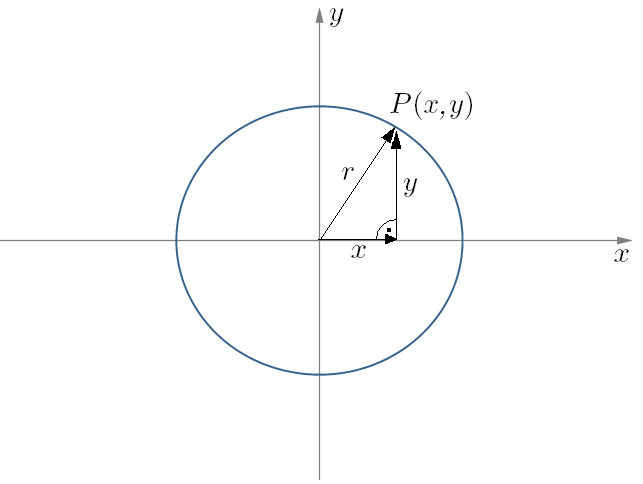
\includegraphics[scale=0.25]{img/kreis/kreis.png}
\end{center}

\noindent $x,\ y$ und $r$ bilden ein rechtwinkliges Dreieck. Also folgt aus dem Satz von Pythagoras (mit dem Mittelpunkt $M = \left({}^0_0\right)$):
\[ x^2 + y^2 = r^2 \]

\noindent Der Mittelpunkt des Kreises muss jedoch nicht zwingend der Ursprung des Koordinatensystems sein, sodass bei einer Verschiebung des Kreises in x- bzw. y-Richtung die folgende  Koordinatengleichung ensteht:
\[ (x - x_M)^2 + (y - y_M)^2 = r^2 \]

\noindent Ein wichtiger Begriff (grade f"ur die komplexen Zahlen (Kapitel~\ref{chap:complex}) sowie die Sinus- und Cosinusfunktionen (Abschnitt~\ref{sec:trigonometrie})) ist der Einheitskreis. Der Einheitskreis ist ein normaler Kreis um den Ursprung mit dem Radius $r=1$:
\[ x^2 + y^2 = 1 \]

\subsection{Funktionsgleichung}
Durch Umformen der Koordinatengleichung erh"alt man zwei Funktionsgleichungen zur Beschreibung des Kreises. Zum einen f"ur den oberen Teilbogen:
\[ y = y_M + \sqrt{ r^2 - (x - x_M)^2} \]
und f"ur den unteren Teilbogen:
\[ y = y_M - \sqrt{ r^2 - (x - x_M)^2} \]

\subsection{Beispiele}
\begin{enumerate}
    \item Der Einheitskreis mit Radius $r = 1$ um den Ursprung $M = (0 , 0)$:

\begin{center}
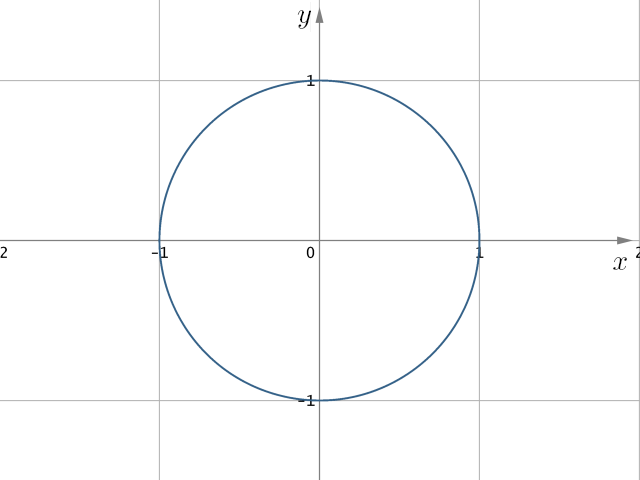
\includegraphics[scale=0.2]{img/kreis/kreis1.png}
\end{center}

Koordinatengleichung:
\[x^2 + y^2 = 1 \]

\item Kreis mit Radius $r = \sqrt 2$ und Mittelpunkt $M = (\sqrt 2 , \sqrt 2)$:

\begin{center}
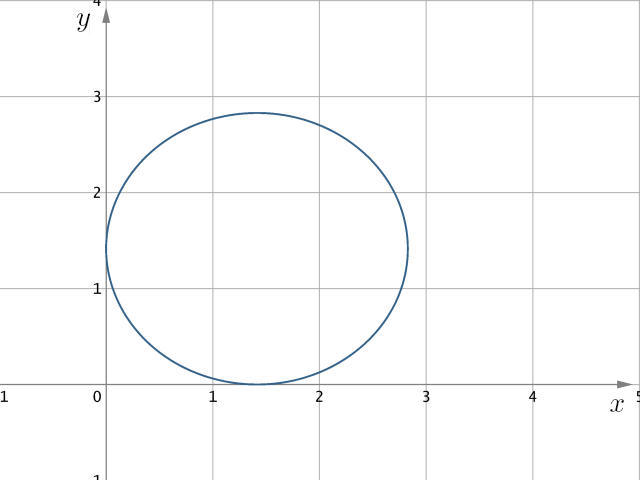
\includegraphics[scale=0.2]{img/kreis/kreis2.png}
\end{center}

Koordinatengleichung:
\[(x - \sqrt 2)^2 + (y - \sqrt 2)^2 = 2 \]


\item Oberer Halbkreis mit Radius $r = 1.5$ und Mittelpunkt $M = (4 , 3)$

\begin{center}
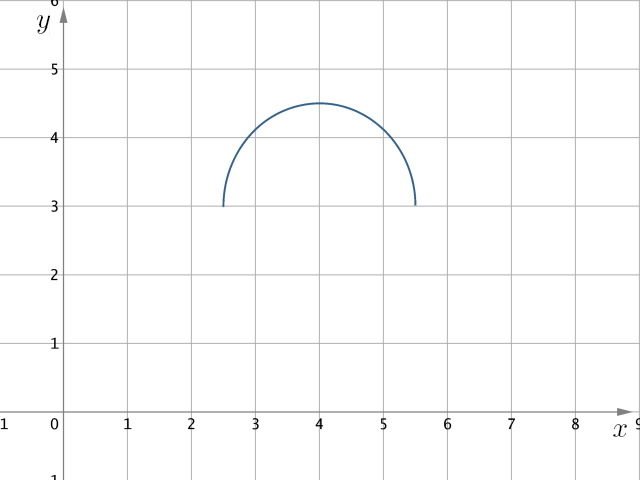
\includegraphics[scale=0.2]{img/kreis/kreis3.png}
\end{center}
Funktionsgleichung: 
\[y = 3 + \sqrt{ 2.25 - (x - 4)^2} \]

\end{enumerate}

\subsection{Aufgaben}
\begin{enumerate}
\item Stellen Sie die Kreisgleichung f"ur einen Kreis mit dem Mittelpunkt M auf, der durch den Punkt $P_1$ geht.
\begin{enumerate}
\item $M(1|3) ; P(4|3)$
\item $M(-1| 5) ; P(6|-4)$
\item $M(-2|-1) ; P(4|3)$
\end{enumerate}
\item Welches geometrische Objekt wird durch die Gleichung beschrieben? Skizzieren Sie dieses in einem Koordinatensystem
\begin{enumerate}
\item $x^2 + y^2 - 4x - 2y + 5 = 4$
\item $x^2 + y^2 + 6x + 2y + 10 = 1$
\end{enumerate}

\item * Geben Sie die Gleichung des Kreises an, der durch die Punkte $P_1(6|7), P_2(2|9) $und $P_3(-1|0)$ geht.

\end{enumerate}


\addtocontents{toc}{\setcounter{tocdepth}{0}}
\section{Ungleichungen}

Autor: Marc Mittner

\noindent "Uberarbeitung: Christian Rutsch

\subsection{Definition}
Eine Ungleichung stellt eine Ordnung zweier mathematischer Objekte dar. Ungleichungen werden bez"uglich der Anzahl der Variablen und der Potenz, in der die Variablen auftreten, unterschieden. Dabei variiert je nach Typ der Ungleichung das L"osungsverfahren.

\subsection{"Aquivalenzumformung von Ungleichungen}
Zur Umformung von Ungleichungen sind folgende Operationen zul"assig:
\begin{itemize}
\item{Addition einer Zahl $a \in \mathbb{R}$ auf beiden Seiten.}
\item{Subtraktion einer Zahl $a \in \mathbb{R}$ auf beiden Seiten.}
\item{Multiplikation/Division mit einer Zahl $a \in \mathbb{R}, a > 0$ auf beiden Seiten.}
\item{Multiplikation/Division mit einer Zahl $a \in \mathbb{R}, a < 0 $ auf beiden Seiten. Dabei ist zu beachten, dass das Ordnungszeichen umgedreht wird!}
\item{Bei Ziehen der Quadratwurzel muss darauf geachtet werden, dass die Ungleichung in zwei Teile zerf"allt:
\begin{align*}
x^2 < a^2 &\Leftrightarrow \\
-a < x < a &\Leftrightarrow \\
 |x| < a &
\end{align*}
(siehe Beispiel bei quadratischen Ungleichungen).}
\end{itemize}
"Anderung der Ordnungszeichen bei Multiplikation/Division mit einer Zahl $ a < 0 $:
\begin{itemize}
\item $ < $ wird zu $ > $, aus $ > $ wird $ < $
\item $ \leq $ wird zu $ \geq $, aus $ \geq $ wird $ \leq $
\item Die Zeichen "`$ = $"' und "`$ \neq $"' bleiben erhalten.
\end{itemize}
Nicht generell erlaubt sind folgende Umformungen:
\begin{itemize}
\item beidseitige Multiplikation mit 0
\item beidseitige Division durch 0
\item beidseitiges Quadrieren 
\end{itemize}


\subsection{Lineare Ungleichungen}
Eine lineare Ungleichung ist eine Ungleichung, in der die Variable nur in der ersten Potenz enthalten ist. Jede lineare Ungleichung kann in eine dieser drei Formen gebracht werden:
\[ax + b > c\quad \text{ oder }\quad
ax + b \geq c\quad \text{ oder }\quad
ax + b \neq c \]


\noindent Zur L"osung einer linearen Ungleichung wird die Variable durch Umformen isoliert:

Beispiel:
\begin{align*}
3 - 4x - 13 + 2x - 3x + 12 &\leq 5 && \text{Zusammenfassen}\\
-5 x + 2 & \leq 5 && |\ -2 \\
-5x &\leq 3 &&|\ \div (-5) \\
 x &\geq - \frac{3}{5}
\end{align*}

Graphische Darstellung des L"osungsbereichs:
\begin{center}
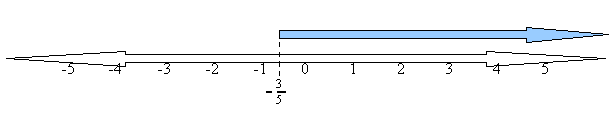
\includegraphics[width=0.8\textwidth]{img/ungleichungen/LBer1.png}
\end{center}

Allgemein:
\begin{align*}
ax + b &\leq c &&| -b\\
ax &\leq c - b &&|\div a ~(a > 0) \\
x &\leq \frac {c - b} a
\end{align*}


\subsection{Quadratische Ungleichungen}

Bei quadratischen Ungleichungen k"onnen Variablen auch in der zweiten Potenz
auftreten. Jede quadratische Ungleichung kann in eine der Formen 
\[x^2 + px + q > r 
\quad \text{oder} \quad
x^2 + px + q \geq r 
\quad \text{oder} \quad
x^2 + px + q \neq r \]
zusammengefasst werden.

\noindent Zur L"osung wird das Verfahren der quadratischen Erg"anzung verwendet.
Bei diesem Verfahren wird zur normierten Form der quadratischen Ungleichung 
\[x^2 + px + q > r\] der Teil $x^2 + px$ zu einer binomischen Formel erweitert.

Allgemein:
\begin{align*}
x^2 + px + q &< r &&|-q
\intertext{Quadratische Erg"anzung:}
x^2 + px &< r - q &&|+ \left(\frac{1}{2} p \right)^2\\
x^2 + px + \left(\frac{1}{2} p \right)^2 &< r - q + \left(\frac{1}{2} p \right)^2 && \text{Binom} \\
\left(x + \frac{1}{2} p \right)^2 &< r - q + \left(\frac{1}{2} p \right)^2\\
|x + \frac{1}{2} p| &< \sqrt{ r - q + \left(\frac{1}{2} p \right)^2}
\end{align*}

Daraus folgen die beiden L"osungen:
\begin{align*}
x_1 &< \phantom{-}\sqrt{r  - q + \left(\frac{1}{2} p \right)^2} - \frac{1}{2} p\\
x_2 &> -\sqrt{r - q + \left(\frac{1}{2} p \right)^2} - \frac{1}{2} p
\end{align*}
Somit erh"alt man die p-q-Formel f"ur quadratische Gleichungen in normierter Form ($r = 0$):
\[x_{1,2} = - \frac p 2 \pm \sqrt{ \left( \frac p 2 \right)^2 - q}\]

\paragraph*{Beispiel:}
\begin{align*}
5x^2 + 12 - 12x - 3x^2 &\geq 26 &&\text{Zusammenfassen}\\
2x^2 - 12x + 12 &\geq 26 &&\text{Normieren} \\
x^2 - 6x + 6 &\geq 13 &&|-6 \\
\intertext{Quadratische Erg"anzung:}
x^2 - 6x &\geq 7 &&|+9\\
x^2 - 6x + 9 &\geq 16 &&\text{2. binom. Formel}\\
(x - 3)^2 &\geq 16
\intertext{Die Ungleichung zerf"allt in zwei Teile:}
|x - 3| &\geq 4 
\intertext{1. Fall:}
x_1 - 3 &\geq 4\\
x_1 &\geq 7
\intertext{2. Fall:}
-x_2 + 3 &\geq 4\\
x_2 &\leq -1
\end{align*}

Graphische Darstellung des L"osungsbereichs:
\begin{center}
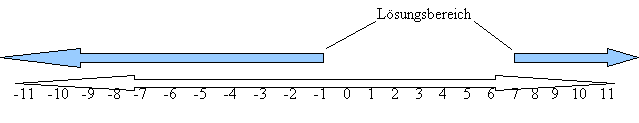
\includegraphics[width=0.8\textwidth]{img/ungleichungen/LBer2.png}
\end{center}

\subsection{Ungleichungen h"oherer Ordnung}

Zum L"osen von Ungleichungen h"oherer Ordnung eignet sich wegen der Komplexit"at der Gleichungen meist nur die Darstellung der Gleichung als Produkt in der Form: 
\[(x - a_1) \cdot (x - a_2) \cdot \ldots \cdot (x - a_n) > 0 \]
Die analytische Berechnung der Nullstellen ist aber nicht immer m"oglich. Lediglich bei Ungleichungen der Ordnung drei ist diese Faktorisierung noch praktikabel.

\subsection{Bruchungleichungen}

Bei Bruchungleichungen ist darauf zu achten, dass zuerst der Definitionsbereich festgestellt werden muss, da eine Division durch Null nicht zul"assig ist. Dazu werden alle Belegungen der Variablen, die eine solche Division verursachen w"urden, aus dem Definitionsbereich entnommen.

\subsubsection{L"osen von Bruchungleichungen}

Zum L"osen von Bruchungleichungen benutzt man folgende Vorgehensweise:
\begin{enumerate}
\item Multiplikation beider Seiten mit dem Hauptnenner
\item Ausmultiplizieren
\item L"osen der entstehenden (quadratischen) Ungleichung
\end{enumerate}

\subsubsection{Beispiel}

\begin{align*}
\frac{(3x - 2)} {(x + 2)} + \frac{(2 + 5x)} {(x^2 - 4)} &\leq \frac{(x + 3)} {(x - 2)}\\
\intertext{Definitionsbereich $ D = \mathbb{R} \setminus \lbrace -2 , +2 \rbrace $}
\intertext{Multiplikation mit dem Hauptnenner $ (x + 2)(x - 2) = (x^2 - 4) $:}
\frac{(3x - 2)} {(x + 2)} \cdot (x^2 - 4) + \frac {(2 + 5x)} {(x^2 - 4)} \cdot (x^2 - 4) &\leq \frac{(x + 3)} {(x - 2)} \cdot (x^2 - 4)\\
(3x - 2)(x - 2) + 2 + 5x &\leq (x + 3)(x + 2)\\
\intertext{Ausmultiplizieren:}
3x^2 - 8x + 4 + 2 + 5x &\leq x^2 + 5x + 6\\
\intertext{L"osen der entstandenen quadratischen Gleichung:}
 2x^2 - 8x &\leq 0 \\
 x^2 - 4x) &\leq 0 \\
 x^2 - 4 x + 4 &\leq 4 \\
 |x - 2| &\leq 2 \\
x &\leq 4 \\
 x &\geq 0
\end{align*}
L"osung für die Ungleichung sind somit alle $ x $ mit $ 0 \leq x \leq 4 $ außer $ x = 2 $, da diese Belegung nicht im Definitionsbereich liegt und somit auch nicht im L"osungsbereich liegen kann.
$L = \lbrace x \in \mathbb{R}\ |\ 0 \leq x \leq 4 ,x \neq 2\rbrace $

Graphische Darstellung des L"osungsbereichs:
\begin{center}
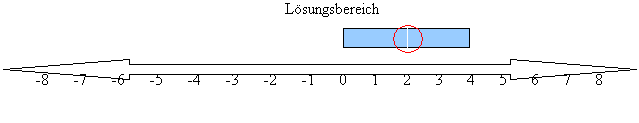
\includegraphics[width=0.8\textwidth]{img/ungleichungen/LBer3.png}
\end{center}

\subsection{Ungleichungen mit mehreren Variablen}

Ungleichungen mit mehreren Variablen haben statt einem eindimensinalen einen mehrdimensinalen L"osungsbereich. Die Dimension nimmt mit der Anzahl der Variablen zu. So hat ein Ungleichungssystem mit zwei Variablen eine L"osung im $ \mathbb{R}^2 $ (also in einer Ebene) und Ungleichungssysteme mit $n$ Variablen haben eine L"osung im $\mathbb{R}^n$.

\subsubsection{Beispiel: Ungleichung mit 2 Variablen}

\begin{align*}
2x^2 + 3 - y - 2 &> 2 \\
2 - \frac{1}{2} x &< \frac{1}{2} y + 2
\end{align*}

Zum L"osen des Ungleichungssystems wird zuerst eine Variable isoliert.
\begin{align*}
y &< 2x^2 - 1 \\
y &> -x
\end{align*}

Dadurch ergibt sich nun:
\[ 2x^2 - 1 > y > -x \]

%\newpage
Graphische Darstellung des L"osungsbereichs:
\begin{center}
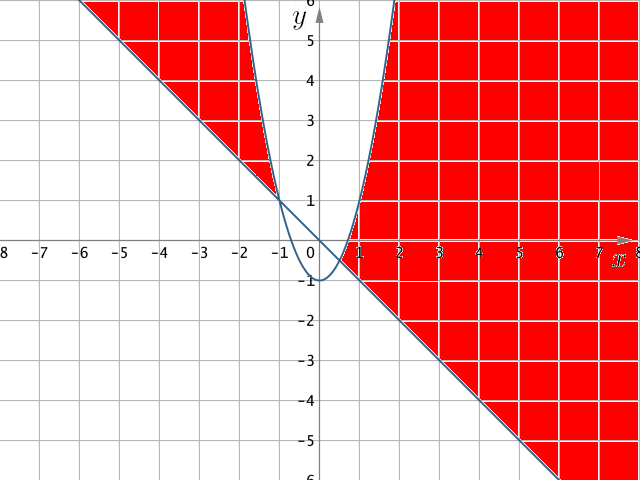
\includegraphics[width=0.5\textwidth]{img/ungleichungen/UGlsystmit2.png}
\end{center}

Der markierte Bereich stellt den L"osungsbereich dar. \\
Die Punkte auf den Funktionen selbst sind nicht im L"osungsbereich enthalten. \\
F"ur den Bereich $ -1 \leq x \leq \frac{1}{2} $ existiert keine L"osung. \\
F"ur alle anderen Werte von $x$ sind alle Punkte, f"ur die die Bedingung
\[ 2x^2 - 1 > y > -x \] erf"ullt ist, in der L"osungsmenge enthalten.

\subsection{Quellen}
\small
\begin{itemize}
\item{\url{http://ilias.tfh-wildau.de/~laborwww/downloads/Kap2_komplett.pdf}}
\item{Wikipedia: L"osen von Ungleichungen}
\item{\url{ftp://ftp.fernuni-hagen.de/pub/fachb/mathe/alggeo/schulte/1011C3.pdf} \linebreak (nicht mehr verfügbar)}
\end{itemize}
\normalsize

\subsection{Aufgaben}

\subsubsection{Ungleichungen mit einer Variablen}
L"osen Sie folgende Ungleichungssysteme analytisch:
\begin{enumerate}\abovedisplayskip-1em
\item{ \begin{align*}(x+1)(x-1) &\leq 0\\ \sqrt{x} &\geq 1\end{align*}}
\item{ \begin{align*}\sqrt{\frac{1}{2}x^3 +2x^2 +\frac{21}{8}x + \frac{9}{8}} < \sqrt{\frac{1}{2}x^2 + \frac{3}{2}x+\frac{9}{8}} \end{align*} }
\item{ \begin{align*}\frac{1}{2}x^2-1 &> 0\end{align*}}
\item{ \begin{align*}x^3 +3x^2 -4 &> 0\end{align*}}
\item{ \begin{align*}x^3 +3x^2 +3x +1 &< 0\end{align*}}
\item{ \begin{align*}x^6 -6x^5 + 15x^4 -20x^3 +15x^2 -6x +1 &\leq 0\end{align*}}
\item{ \begin{align*}\frac{1}{2}x^2 -8 &> 0\\-3(x-1)^2 +12 &> 0\end{align*}}
\item{ \begin{align*}(x^2-2)(x+1) &\geq 0\end{align*}}
\item{\abovedisplayskip1em Geben Sie die L"osungsmenge des Ungleichungssystems in Abh"angigkeit von \textit{a} an.\begin{align*}ax^2 &> 0\\ \frac{1}{2}x + 1 &> 0\end{align*}}
\item{\abovedisplayskip1em Geben Sie die L"osungsmenge des Ungleichungssystems in Abh"angigkeit von \textit{a} an. \begin{align*}x^2 + a &> 0\\ \frac{1}{2}x +1 &> 0\end{align*}}
\item{\abovedisplayskip1em Geben Sie die L"osungsmenge des Ungleichungssystems in Abh"angigkeit von \textit{a} an. \begin{align*}-x^2 +a &< 0\\ x+a &< 0\end{align*}}
\item{\abovedisplayskip1em Geben Sie die L"osungsmenge des Ungleichungssystems in Abh"angigkeit von \textit{a} an. \begin{align*}4x^2-2ax+\frac{1}{4}a^2 &\geq 0\end{align*}}
\item{ \begin{align*}x^3+x^2-2x &\geq 2\end{align*}}
\item{ \begin{align*}(x-1)^2 -4 &< 0\\ -(x+1)^2 +4 &> 0\end{align*}}
\item{ \begin{align*}\sqrt{(x-1)} &\geq 0\\ -\frac{1}{4x}+4 &< 0\end{align*}}
\item{ \begin{align*}x^4-16 &\leq 0\\ x^3 +1 &\geq 0\end{align*}}
\end{enumerate}

\subsubsection{Ungleichungen mit mehreren Variablen}
L"osen Sie folgende Ungleichungssysteme graphisch:
\begin{enumerate}\abovedisplayskip-1em
\item{ \begin{align*}x^2 +y^2 &< 25\\ \frac{1}{2}x +\frac{5}{2} &> y\\ -x-5 &< y\end{align*}}
\item{ \begin{align*}-x^2 +5 &< y\\ x(x-3)^2 &> y\\ -x-2 &> y\end{align*}}
\item{ \begin{align*}3x^2-3x-10 &< -4 +y\\ y &\leq \frac{1}{2}\end{align*}}
\item{ \begin{align*}y &< \frac{2x^2+3x+4}{-x^4-2x^3-x^2+4x+(2x+x^2)^2}\\ -\frac{1}{x} &< y\\ -(\frac{1}{\sqrt{2}}x)^2 &< y - \frac{1}{2}x^2 + \frac{1}{2}x +2\\ y+x-2<0\end{align*}}
\item{ \begin{align*}\frac{1}{2}x^2 - 3x &\leq y\\ y &\leq -x\\ 17x^3 - \frac{1}{2} &= y\end{align*}}
\item{ \begin{align*}y + \sqrt{\frac{x^3 + x^2 - x - 1}{x - 1}} &> 0\\ \frac{2}{20}x - \frac{1}{3}y + \frac{3}{12} &< 0\end{align*}}
\item{ \begin{align*}\frac{1}{2} - 2 &< y\\ \frac{1}{2} + 2 &> y\\ 2x - 4 &< y\\ 2x + 4 &> y\\ -\frac{1}{2} - 2 &< y\\ -\frac{1}{2} + 2 &> y\\ -2x - 4 &< y\\ -2x + 4 &> y\end{align*}}
\item{ \begin{align*}|(x^2 + (y-1)^2)| &= 4\\ x &\geq y\end{align*}}
\item{ \begin{align*}((\sin{x})+\frac{1}{2})^2 - \frac{3}{4} - y - (\sin{x})^2 &> 0\\ \cos{(x+\frac{\pi}{2})} + \frac{1}{2} &< y\end{align*}}
\item{ \begin{align*}\left| \frac{1}{x} \right| &> y\\ -\frac{1+7x^2}{x^2y} &> -\frac{y + 7}{y}\\ |x|+y &< 5\end{align*}}
\item{ \begin{align*}4x^2 + y^2 &\leq 16\\ x^2 + 4y^2 &\leq 16\end{align*}}
\item{ \begin{align*}(y-2)^2 &< 4 - (x-2)^2\\ y-2 &< 0\\ |x-2|+2 &< y\end{align*}}
\item{\abovedisplayskip1em Berechnen Sie f"ur die Ungleichung den Fl"acheninhalt der L"osungsmenge: \begin{align*}(2y-3)^2 +(3y+2)^2+y-10 &\geq \left|\frac{4x+4(\frac{1}{2}x-\frac{3}{2})^2-9}{x}\right|+13y^2\\ y &\leq -1\end{align*}}
\item{\abovedisplayskip1em Berechnen Sie f"ur das Ungleichungssystem den Fl"acheninhalt der L"osungsmenge: \begin{align*}f:& &x^2 - 4x + 4 + y^2 -2y + 1 &\geq 1\\ g:& &(x-2)^2 + (y-2)^2 &\leq 4\\ h:& &(x-2)^2 + (y-3)^2 &\geq 1\end{align*}}
\item{\abovedisplayskip1em F"ur welches \textit{a} ist der Fl"acheninhalt der L"osungsmenge gleich 2? \begin{align*}y &\geq 2\\ -|x|+a &\leq y\end{align*}}
\item{\abovedisplayskip1em Bestimmen Sie ein \textit{a} und ein \textit{b}, f"ur das der Fl"acheninhalt der L"osungsmenge 2$\pi$ ergibt! \begin{align*}-\frac{1}{3}x &\leq y-2\\ (x+\frac{1}{4}b)^2 + (y-\frac{3}{2}a)^2 &\leq a^2\end{align*}}
\item{\abovedisplayskip1em Beschreiben Sie die L"osungsmenge des Ungleichungssystems: \begin{align*}x^2 + y^2 + z(z+2) &< 8\\ x &\leq 0\\ y &\leq 0\end{align*}}
\item{\abovedisplayskip1em Beschreiben Sie die L"osungsmenge des Ungleichungssystems: \begin{align*}(x-2\sqrt{3})^2 + (y-2\sqrt{3})^2 + (z-2\sqrt{3})^2 &\leq 36\\ (x+2\sqrt{3})^2 + (y+2\sqrt{3})^2 + (z+2\sqrt{3})^2 &\leq 36\end{align*}}
\end{enumerate}



\chapter{Vollständige Induktion}
\label{Induktion}
Autor: Katja Matthes

\noindent "Uberarbeitung: Sebastian Nielebock
%%%%%%%%%%%%%%%%%%%%%%%%%%%%%%%%%%%%%%%%%%%%%%%%%%%%%%%%%%%%%%
%%%Prinzip
%%%%%%%%%%%%%%%%%%%%%%%%%%%%%%%%%%%%%%%%%%%%%%%%%%%%%%%%%%%%%%
\section{Prinzip}
Vollständige Induktion ist eine mathematische Beweismethode. Das Ziel der voll"-stän"-digen Induktion besteht darin, die Gültigkeit einer Aussage für alle natür"-li"-chen Zahlen $ n \geq n_{0} \in \mathbb{N}_{0} $ (Induktionsanfang) nachzuweisen.
%%%Erkl�rung
\begin{enumerate}
%%%Induktionsanfang
	\item \textbf{Induktionsanfang} \\
	Man zeigt, dass die Aussage für die natürliche Zahl $ n_{0} = 1 $ (oder auch $ n_{0} = 0,2,3, ... $) gilt.
%%%Induktionsschritt
	\item \textbf{Induktionsschritt}
		\begin{itemize}
			\item Induktionsvoraussetzung:
			Es wird angenommen, dass die Aussage für eine feste natürliche Zahl $ n $ gilt.
			\item Induktionsbehauptung: Es wird behauptet, dass die Aussage unter der Voraussetzung auch für die nachfolgende natürliche Zahl $ n+1 $ gilt.
			\item Induktionsbeweis: Die Induktionsbehauptung wird unter Verwendung der Induktionsvoraussetzung bewiesen.
		\end{itemize}
%%%Induktionsschluss	 
	\item \textbf{Schlussfolgerung} \\
	Aus dem Verbund von Verankerung und Vererbung folgt, dass die Aussage tatsächlich für alle natürlichen Zahlen $ n \geq n_{0} $ gilt.
\end{enumerate}
%%%%%%%%%%%%%%%%%%%%%%%%%%%%%%%%%%%%%%%%%%%%%%%%%%%%%%%%%%%%%%
%%%Erklärung Summen- und Produktzeichen
%%%%%%%%%%%%%%%%%%%%%%%%%%%%%%%%%%%%%%%%%%%%%%%%%%%%%%%%%%%%%%
\section{Einschub: Das Summen- und Produktzeichen}
Viele Aufgaben in der Induktion sind mit Summen- und Produktzeichen formuliert. Um einen Teil der Beweise besser führen zu können, ist es notwendig einige Regeln für diese Symbole zu kennen.

\subsection{Allgemein}
Das Summen- bzw. das Produktzeichen stellen jeweils eine Verkürzung für die Addition bzw. Multiplikation dar:
\[\sum_{i=1}^{n}{a_{i}} = a_{1} + a_{2} + \cdots + a_{n} \ ;\ \prod_{i=1}^{n}{a_{i}} = a_{1} \cdot a_{2} \cdot \ \cdots\ \cdot a_{n} \]

\subsection{Letzten Index ausklammern}
Eine sehr nützliche Regel zum Induktionsbeweis ist das Ausklammern des letzten Index. Für viele Beweise lässt sich so der Induktionsschritt leicht zeigen:
\[\sum_{i=l}^{n+1}{a_{i}} = \left(\sum_{i=l}^{n}{a_{i}}\right) + a_{n+1}\ ;\ \prod_{i=l}^{n+1}{a_{i}} = \left(\prod_{i=l}^{n}{a_{i}}\right) \cdot a_{n+1}\]

\subsection{Assoziativgesetz}

\[\sum_{i=l}^{m-1}{a_{i}} + \sum_{i=m}^{n}{a_{i}} = \sum_{i=l}^{n}{a_{i}}\ ;\ \prod_{i=l}^{m-1}{a_{i}} \cdot \prod_{i=m}^{n}{a_{i}} = \prod_{i=l}^{n}{a_{i}}\]

\subsection{Kommutativgesetz}

\[\sum_{i=m}^{n}{a_{i}} = \sum_{i=m}^{n}{a_{m+n-i}}\ ;\ \prod_{i=m}^{n}{a_{i}} = \prod_{i=m}^{n}{a_{m+n-i}}\]

\subsection{Verbindung zweier Summen- bzw. Produktzeichen}

\[ \sum_{i=m}^{n}{a_{i}} + \sum_{i=m}^{n}{b_{i}} = \sum_{i=m}^{n}{\left(a_{i} + b_{i}\right)} \ ; \ \prod_{i=m}^{n}{a_{i}} \cdot \prod_{i=m}^{n}{b_{i}} = \prod_{i=m}^{n}{\left(a_{i} \cdot b_{i}\right)}\]

\subsection{Doppelsummen bzw. Doppelprodukte}

\[ \sum_{i=m}^{n}\sum_{j=k}^{l}{a_{i j}} = \sum_{j=k}^{l}\sum_{i=m}^{n}{a_{i j}} \ ; \ \prod_{i=m}^{n}\prod_{j=k}^{l}{a_{i j}} = \prod_{j=k}^{l}\prod_{i=m}^{n}{a_{i j}}\]

%%%%%%%%%%%%%%%%%%%%%%%%%%%%%%%%%%%%%%%%%%%%%%%%%%%%%%%%%%%%%%
%%%Beispiel
%%%%%%%%%%%%%%%%%%%%%%%%%%%%%%%%%%%%%%%%%%%%%%%%%%%%%%%%%%%%%%
\section{Beispielaufgabe}
Zeigen Sie: Für alle $ n \in \mathbb{N} $ gilt die Gleichung 
\[\sum_{k=1}^{n} 2^k = 2(2^n - 1)\]
%%Induktionsanfang
\subsection{Induktionsanfang}
Wir zeigen, dass die Aussage richtig ist für $ n_0 = 1 $.
	\[\sum_{k=1}^{1} 2^k = 2^1 = 2 = 2(2^1 - 1) \] (wahre Aussage)
%%%Induktionsschritt
\subsection{Induktionsschritt}
%%%Voraussetzung
\textbf{Induktionsvoraussetzung}: Wir nehmen an, dass die Annahme gültig ist für ein festes $ n \in \mathbb{N} $
	\[\sum_{k=1}^{n} 2^k = 2(2^n-1)\]
%%%Behauptung	
\textbf{Induktionsbehauptung}: Wir behaupten, dass dann die Aussage auch für die nachfolgende Zahl $ n+1 $ $(n \mapsto n+1) $ gilt.
	\[\sum_{k=1}^{n+1} 2^k = 2(2^{n+1} - 1)\]
%%%Beweis	
\textbf{Induktionsbeweis}: Mit Hilfe der Induktionsvorraussetzung wird die linke Seite der Behauptung in deren rechte Seite umgewandelt.
\begin{align*}
	\sum_{k=1}^{n+1} 2^k 	&= \sum_{k=1}^{n} 2^k + 2^{n+1}		&& \text{\textbar nach Voraussetzung} 	\\
												&= 2(2^n - 1) + 2^{n+1} 					&& \text{\textbar Potenzgesetze} 			\\
												&= 2(2^n-1)+2\cdot2^n 						&& \text{\textbar 2 ausklammern} 			\\
												&= 2(2^n - 1 + 2^n) 							&& \text{\textbar zusammenfassen} 			\\
												&= 2(2 \cdot 2^n - 1) 						&& \text{\textbar Potenzgesetze} 			\\
												&= 2(2^{n+1} - 1)											
\end{align*}
%%%Induktionsschluss	
\subsection{Induktionsschluss}
Damit ist durch das Prinzip der vollständigen Induktion die Induktionsbehauptung und damit auch die Aussage: 
	\[\sum_{k=1}^{n} 2^k = 2(2^n - 1)\]
 für alle $ n \in \mathbb{N} $ bewiesen.
\begin{center}
qed.
\end{center}

%%%%%%%%%%%%%%%%%%%%%%%%%%%%%%%%%%%%%%%%%%%%%%%%%%%%%%%%%%%%%%
%%%Literatur
%%%%%%%%%%%%%%%%%%%%%%%%%%%%%%%%%%%%%%%%%%%%%%%%%%%%%%%%%%%%%%
\section{Literatur}
\begin{itemize}
	\item Bigalke, Köhler, Kuschnerow, Ledworuski: \textit{Mathematik 11. Leistungsfach}. 1. Auflg. 2001. Cornelsen Verlag, Berlin.
	\item \url{http://www.math.uni-sb.de/ag/wittstock/lehre/WS00/analysis1/Vorlesung/node10.html}
\end{itemize}
%%%%%%%%%%%%%%%%%%%%%%%%%%%%%%%%%%%%%%%%%%%%%%%%%%%%%%%%%%%%%%
%%%Aufgaben
%%%%%%%%%%%%%%%%%%%%%%%%%%%%%%%%%%%%%%%%%%%%%%%%%%%%%%%%%%%%%%
\section{Aufgaben}
%%%Gleichungen
\subsubsection{Gleichungen}
\begin{enumerate}
	\item Die Summe der ersten $ n $ ungeraden natürlichen Zahlen $ 1 + 3 + 5 + ... + 2n-1 $ soll bestimmt werden. Stellen Sie eine Vermutung auf und beweisen Sie diese durch Induktion.
	\item Die Summe von $ 4 + 8 + 12 + ... + 4n $, also der ersten $ n $ durch 4 teilbaren natürlichen Zahlen, soll bestimmt werden. Stellen Sie eine Vermutung auf und beweisen Sie diese durch Induktion.
	\item Beweisen Sie: Die Summe der ersten $ n $ geraden natürlichen Zahlen ist gleich $ n^2 + n $, d.h. 
		\[ \sum_{k=1}^{n} 2k = n^2 + n \]
	\item Beweisen Sie: Für alle $ n \in \mathbb{N} $ gilt die Summenformel 
		\[\sum^n_{k=1} \frac{1}{(2k-1)(2k+1)} = \frac{n}{2n + 1} \]
	\item Beweisen Sie: Für alle $ n \in \mathbb{N} $ gilt die Summenformel
		\[\sum^n_{k=1} \frac{1}{k(k+1)} = \frac{n}{n+1} \]
	\item Beweisen Sie: Für alle $ n \in \mathbb{N} $ gilt die Summenformel
		\[\sum^n_{k=1} k = \frac{n(n+1)}{2} \]
	\item Beweisen Sie: Für alle $ n \in \mathbb{N} $ gilt die Summenformel
		\[\sum_{k=1}^n k^2 = \frac{n(n+1)(2n+1)}{6} \]
	\item Beweisen Sie: Für alle $ n \in \mathbb{N} $ gilt die Summenformel
		\[\sum_{k=1}^n \frac{k}{2^k} = 2 - \frac{n+2}{2^n} \]
	\item Beweisen Sie die Summenformel:
		\[\sum_{k=0}^n \left(\frac{2}{3}\right)^k = 3 \cdot \left(1 - \left(\frac{2}{3}\right)^{n+1}\right) \]
	\item Beweisen Sie: Für alle $ n \in \mathbb{N} $ gilt die Summenformel (mit $ 0 < q < 1 $)
		\[\sum_{k=0}^n q^k = \frac{1 - q^{n+1}}{1 - q} \]
\end{enumerate}
%%%Ungleichungen
\subsubsection{Ungleichungen}
\begin{enumerate}
	\item Beweisen Sie die \textbf{Bernoulli-Ungleichung}: Für alle $ n \in \mathbb{N} $ und $ x \geq -1 $ gilt: $ (1 + x)^n \geq 1 + nx $
	\item Bestimmen Sie die kleinste natürliche Zahl $ n_0 $, für die folgende Ungleichung richtig ist: $ n^2 + 10 < 2^n $. Beweisen Sie, dass die Ungleichung für alle natürlichen Zahlen $ n \geq n_0 $ richtig ist.
	\item Beweisen Sie: Für alle natürlichen Zahlen $ n \geq 3 $ gilt: $ n^2 > 2n + 1 $
	\item Beweisen Sie: Für alle natürlichen Zahlen $ n \geq 5 $ gilt: $ 2^n > n^2 $
	\item Beweisen Sie: Für alle natürlichen Zahlen $ n \geq 2 $ gilt:
		\[\sum_{k=1}^n \frac{1}{\sqrt{k}} > \sqrt{n} \]
	\item Beweisen Sie: Für alle natürlichen Zahlen $ n > 2 $ gilt:
		\[\sum_{k=1}^n \frac{1}{n+k} > \frac{13}{24} \]
\end{enumerate}
%Teilbarkeitsporbleme
\subsubsection{Teilbarkeitsprobleme}
\begin{enumerate}
	\item Beweisen Sie: Für alle natürlichen Zahlen $ n $ ist $ 8 $ ein Teiler von $ 9^n - 1 $
	\item Beweisen Sie: Für alle natürlichen Zahlen $ n $ ist $ 6 $ ein Teiler von $ 7^n - 1 $
	\item Beweisen Sie: Für alle natürlichen Zahlen $ n $ ist $ a - 1 $ ein Teiler von $ a^n - 1 $ mit $ a \in \mathbb{R} $ und $ a > 1 $
	\item Beweisen Sie, dass der Term $ n^3 + 6n^2 + 14n $ für alle natürlichen Zahlen ein Vielfaches von $ 3 $ ist.
	\item Beweisen Sie: Für alle natürlichen Zahlen $ n $ ist $ 3 $ ein Teiler von $ 2^{2n} - 1 $
	\item Beweisen Sie: Für alle natürlichen Zahlen $ n $ ist $ 6 $ ein Teiler von $ n^3 - n $
	\item Beweisen Sie: Für alle natürlichen Zahlen $ n $ ist $ 3n^2 + 9n $ durch $ 6 $ teilbar.
\end{enumerate}
%%%Ableitungen
\subsubsection{Ableitungen}
\begin{enumerate}
	\item Zeigen Sie, dass für die Ableitungen ($2n$)-ten Grades der Funktion $ f(x) = x + a \cdot \cos x $ gilt: $ f^{(2n)}(x) = (-1)^n \cdot a \cdot \cos x $ ($ n \in \mathbb{N}$).
	\item Stellen Sie eine Vermutung über die ungeraden Ableitungen $ f^{(2n+1)}(x) $ der Funktion $ f(x) = x + a \cdot \cos x $ und beweisen Sie diese.
	\item Formulieren Sie eine Formel für  $f^{(2n)}(x)$ mit $f(x) = x + \sin (a \cdot x) $ und $ a > 0 $. Beweisen Sie diese.
	\item Beweisen Sie, dass für $f(x) = \frac{x}{x+1} $ mit $ x \neq -1 $ gilt: \[f^{(n)}(x) = (-1)^{n+1} \cdot \frac{n!}{(x+1)^{n+1}}\ .\]
	\item Formulieren Sie eine Formel für  $f^{(n)}(x)$ mit $f(x) = \frac{x+1}{x-2} $ und $ x \neq -2 $. Beweisen Sie diese.
	\item Sei $f(x) = x^3 + x^2 + x + 1 + \frac{1}{x-1} $. Ab welcher Ableitung kann eine allgemeingültige Formel aufgestellt werden? Vermuten Sie eine Formel und beweisen Sie diese.
	\item Sei $f(x) = \sin \frac{x}{a}$. Stellen Sie eine Formel für die ($2n$)-te Ableitung von $f$ auf und beweisen Sie diese.
\end{enumerate}
\addtocontents{toc}{\setcounter{tocdepth}{1}}
\newcommand{\pitwo}{\frac{\pi}{2}}
\newcommand{\newpar}{\vspace{1em}\noindent}

\chapter{Funktionen}
\label{chap:funktionen}

Autor: Gerhard Gossen

\mbox{}\par
%\section{Definition}
\noindent Eine Funktion $f$ ist eine Abbildung, die einem Wert aus dem \emph{Definitionsbereich $D(f)$} genau einen Wert aus dem \emph{Wertebereich $W(f)$} zuordnet. Die übliche Darstellung ist
$f : X \to Y$ (sprich: $f$ ist eine Abbildung von $X$ nach $Y$), wobei $X$ die Definitionsmenge ($D(f) \subseteq X$) und $Y$ die Zielmenge ist ($W(f) \subseteq Y$). Definitions- und Zielmenge sind oft $\R$ (die reellen Zahlen).

\noindent Verbreitete Funktionen sind z.B. Geraden ($f(x) = m\cdot x +n$), Polynome ($f(x) = a_n x^n + a_{n-1} x^{n-1}+\dots + a_1x+a_0$), die trigonometrischen Funktionen ($\sin x$, $\cos x$, $\tan x$, siehe Abschnitt~\ref{sec:trigonometrie}) oder Exponentialfunktionen ($a^x$, siehe Abschnitt~\ref{sec:exponential}). Abbildung~\ref{fig:funktionen} zeigt die Graphen einiger Funktionen.

\begin{figure}[bth]
\begin{center}
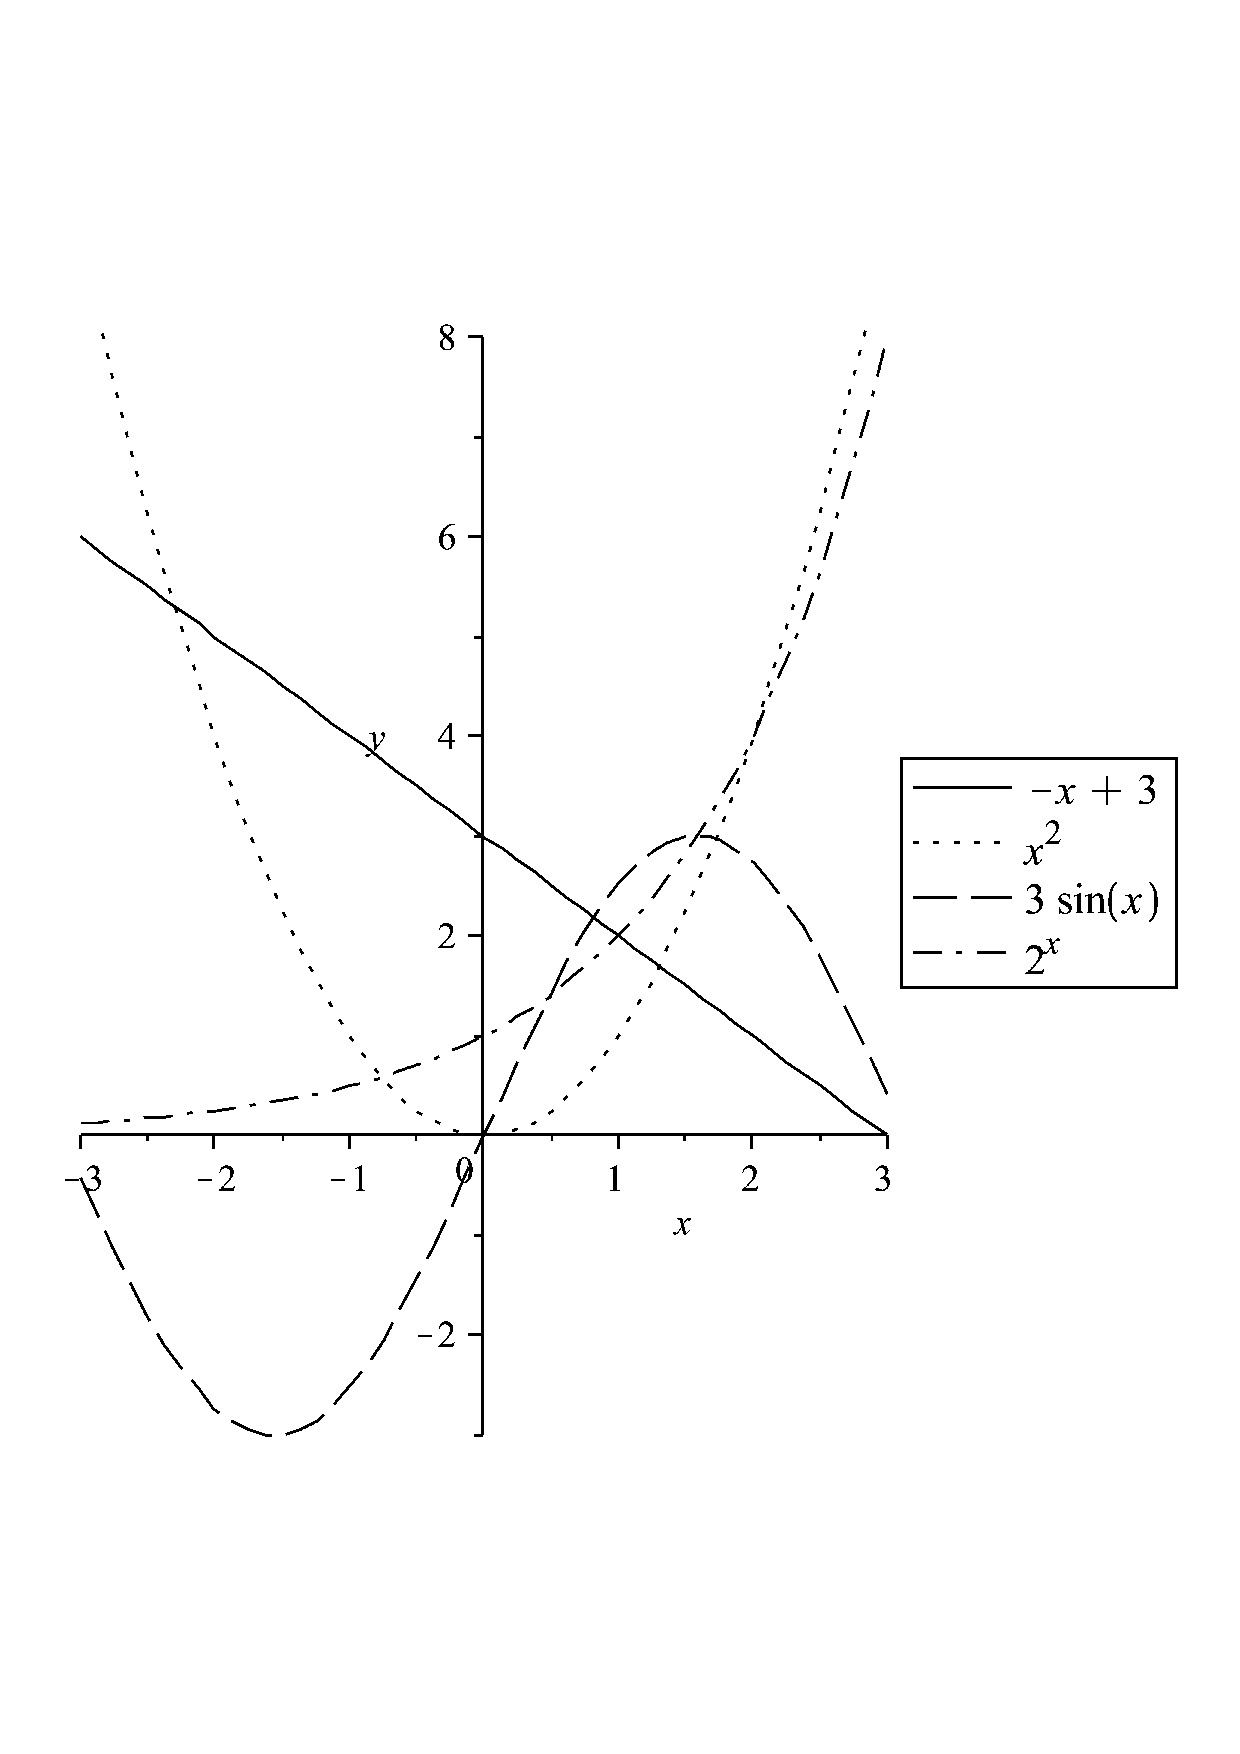
\includegraphics[width=.4\textwidth]{img/Funktionssammlung.pdf}
\end{center}
\caption{Bekannte Funktionen}
\label{fig:funktionen}
\end{figure} 

\noindent Alle Funktionen, die wir im Vorkurs behandeln, sind Funktionen mit \emph{einer Ver"-änderlichen}, also Funktionen, die von einer einzigen Variable (meist $x$) ab"-hän"-gen. Die Eigenschaften einer Funktion kann man über eine \emph{Kurvendiskussion} (siehe Abschnitt~\ref{sec:kurvendiskussion}) herausbekommen. Zuerst werden wir aber zwei wichtige Funktionsfamilien vorstellen: die trigonometrischen Funktionen (Winkelfunktionen, Abschnitt~\ref{sec:trigonometrie}) und die Exponentialfunktionen (Abschnitt~\ref{sec:exponential}).

%%%%%%%%%%%%%%%%%%%%%%%%%%%%%%%%%%%%%%%%%%%%%%%%%%%%%%%%%%%%%%%%%%%%%%%%%%%%%%%%%%%%%%
\section{Trigonometrische Funktionen}
\label{sec:trigonometrie}

Die trigonometrischen Funktionen $\sin, \cos, \tan$ sind die
Winkelfunktionen. Sie sind für Winkel im Bogenmaß definiert (z.\,B. $ x =
\pitwo$). Winkel im Gradmaß (z.\,B. $ x = 90^\circ$) können
eindeutig ins Bogenmaß umgerechnet werden ($90^\circ \equiv \pitwo$).
Deswegen ist auch die Schreibweise $\sin 90^\circ$ möglich.

\subsection{Definition}
Im rechtwinkligen Dreieck gilt:

\begin{minipage}{.5\linewidth}
\begin{eqnarray*}
 \sin x &=& \frac{\text{Gegenkathete}}{\text{Hypothenuse}}\\
 \cos x &=& \frac{\text{Ankathete}}{\text{Hypothenuse}}\\
 \tan x &=& \frac{\text{Gegenkathete}}{\text{Ankathete}} =
\frac{\sin x}{\cos x}
\end{eqnarray*}
\end{minipage}\hspace{.1\linewidth}
\begin{minipage}{.35\textwidth}
 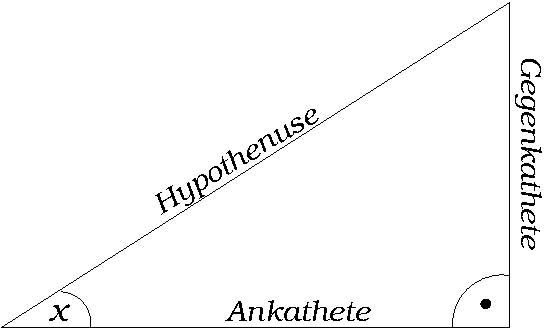
\includegraphics[width=\textwidth]{img/winkel.pdf}
%\vspace{.1em}
\end{minipage}

\noindent Diese Definitionen lassen sich verallgemeinern, so dass die Funktionen für 
alle reellen Zahlen definiert sind (im rechtwinkligen Dreieck:
$0\leq x \leq 90^\circ$). Damit ergeben sich diese Funktionen:
\begin{center}\hfill
\begin{minipage}{.25\textwidth}
 \begin{center}
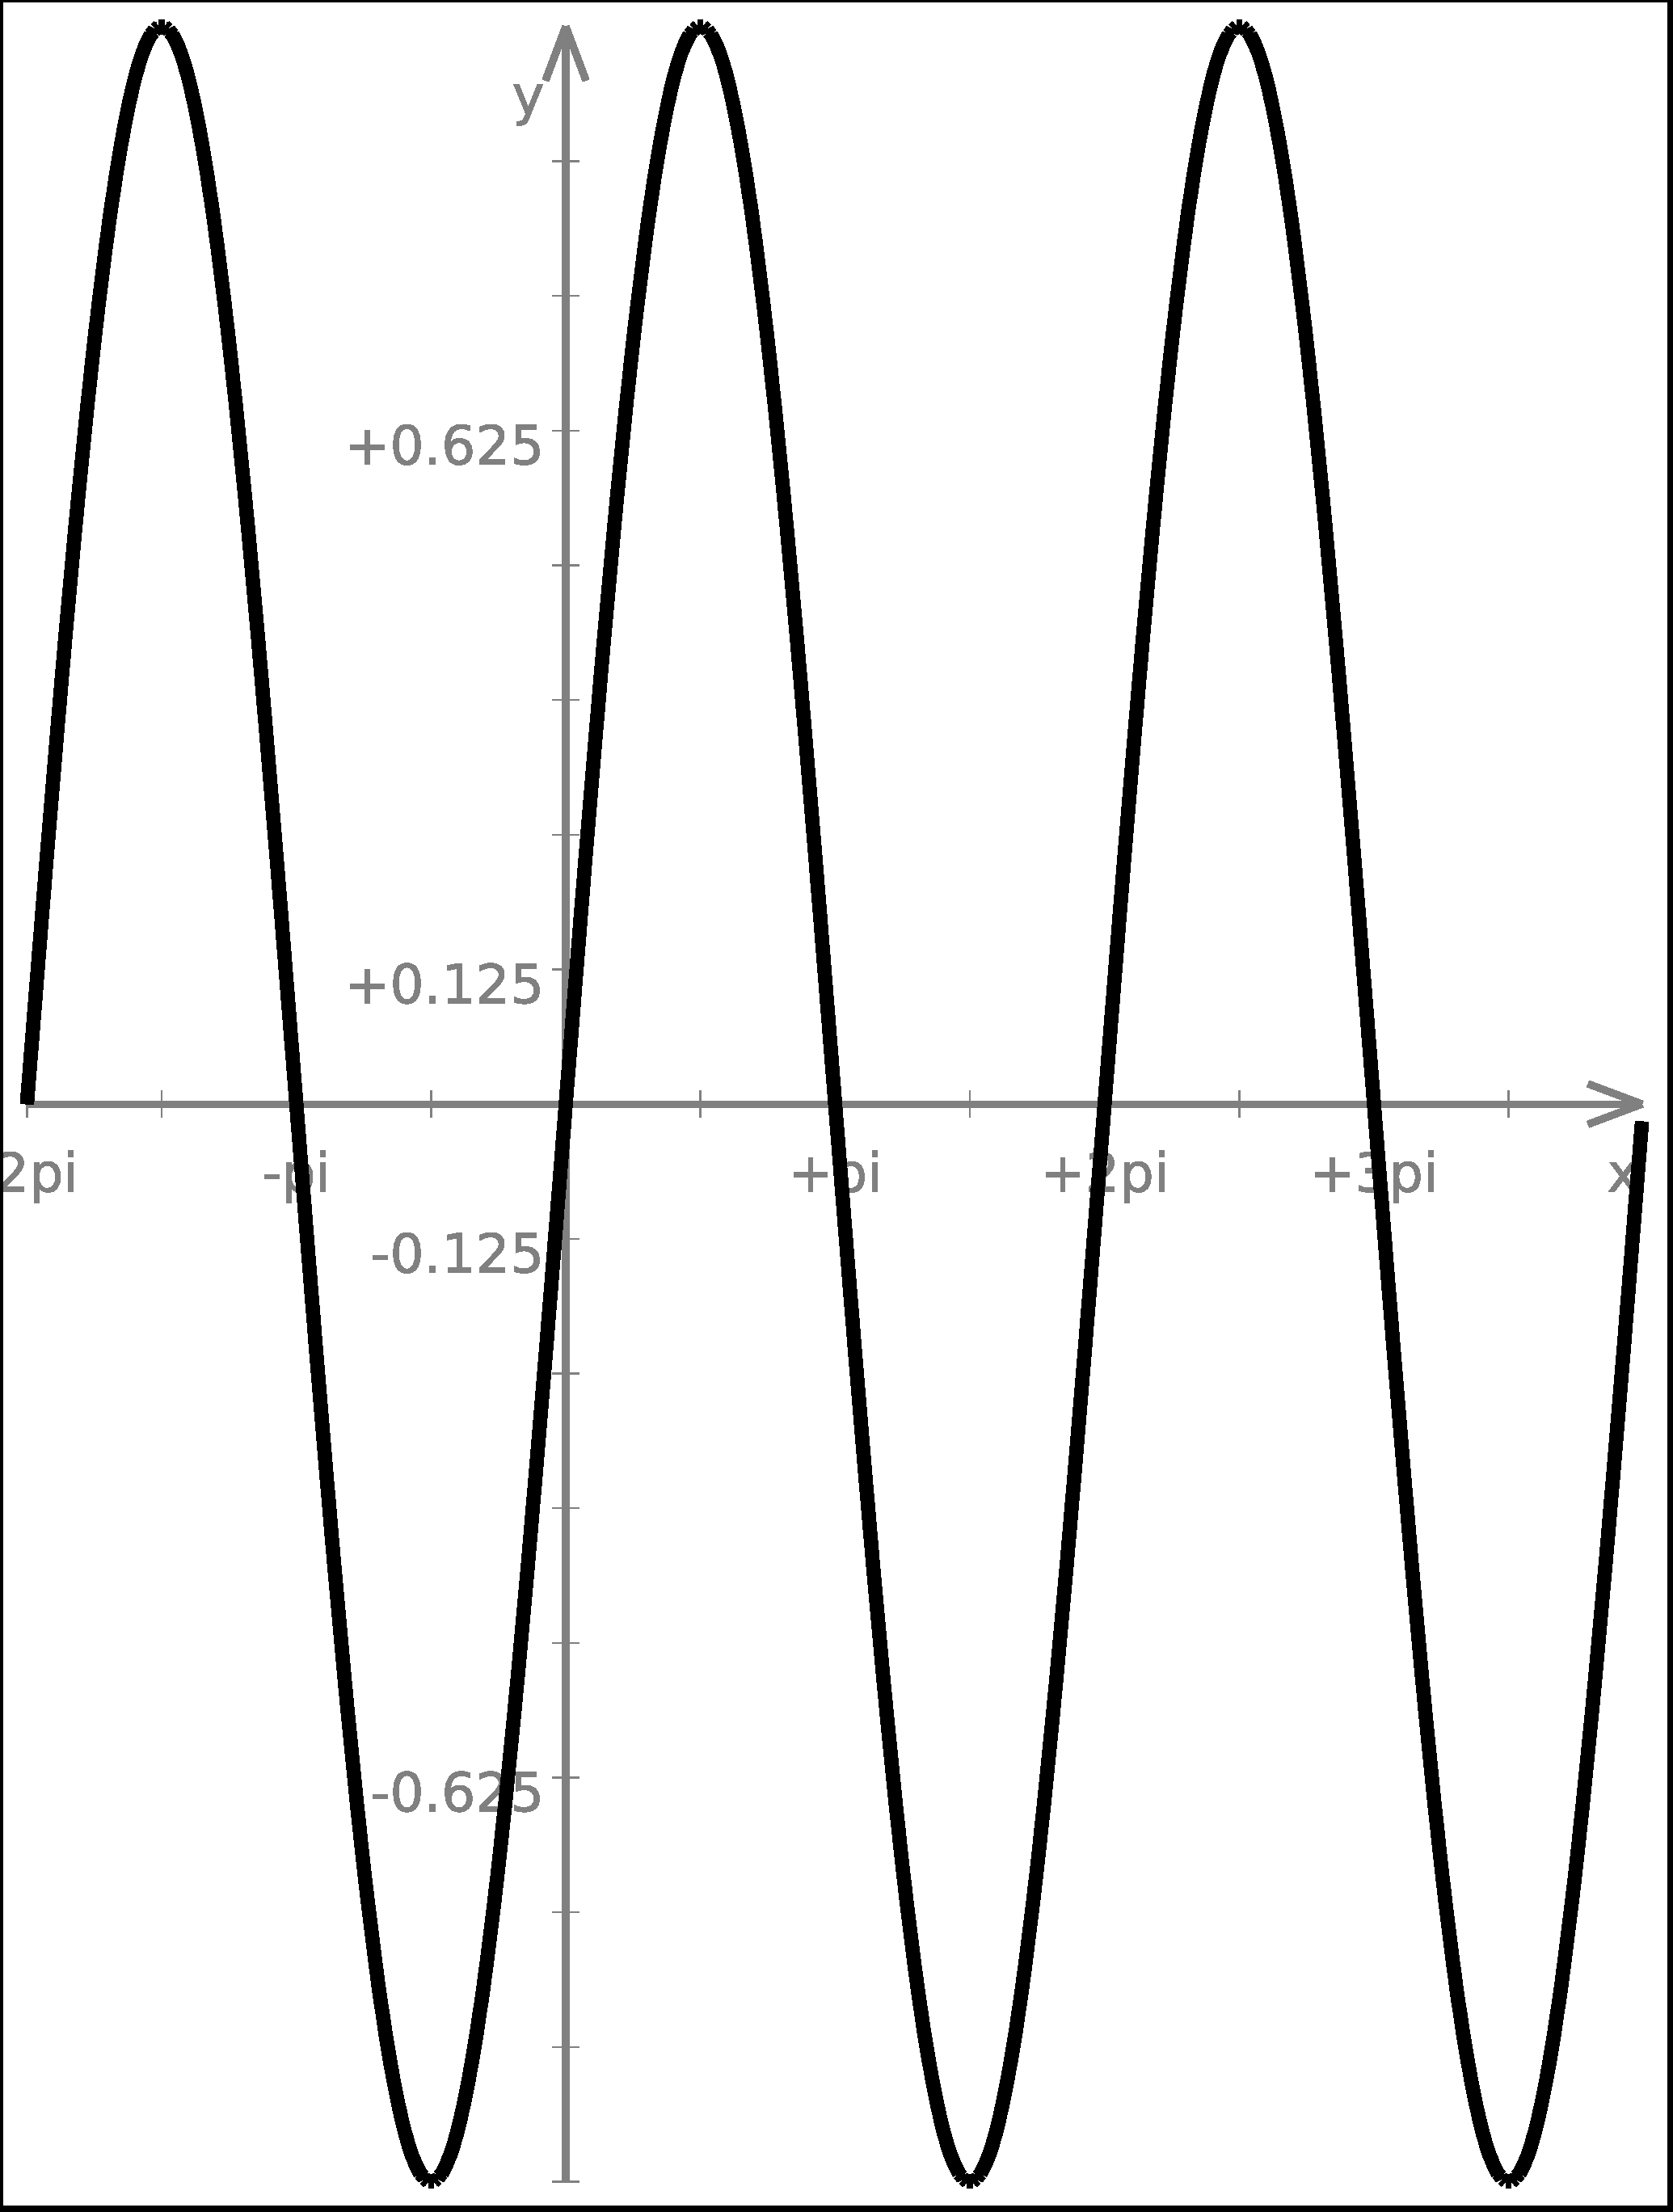
\includegraphics[width=\textwidth, height=2.5cm]{img/sin.pdf}
 $\sin x$         \end{center}
\end{minipage}\hfill
\begin{minipage}{.25\textwidth}
 \begin{center}
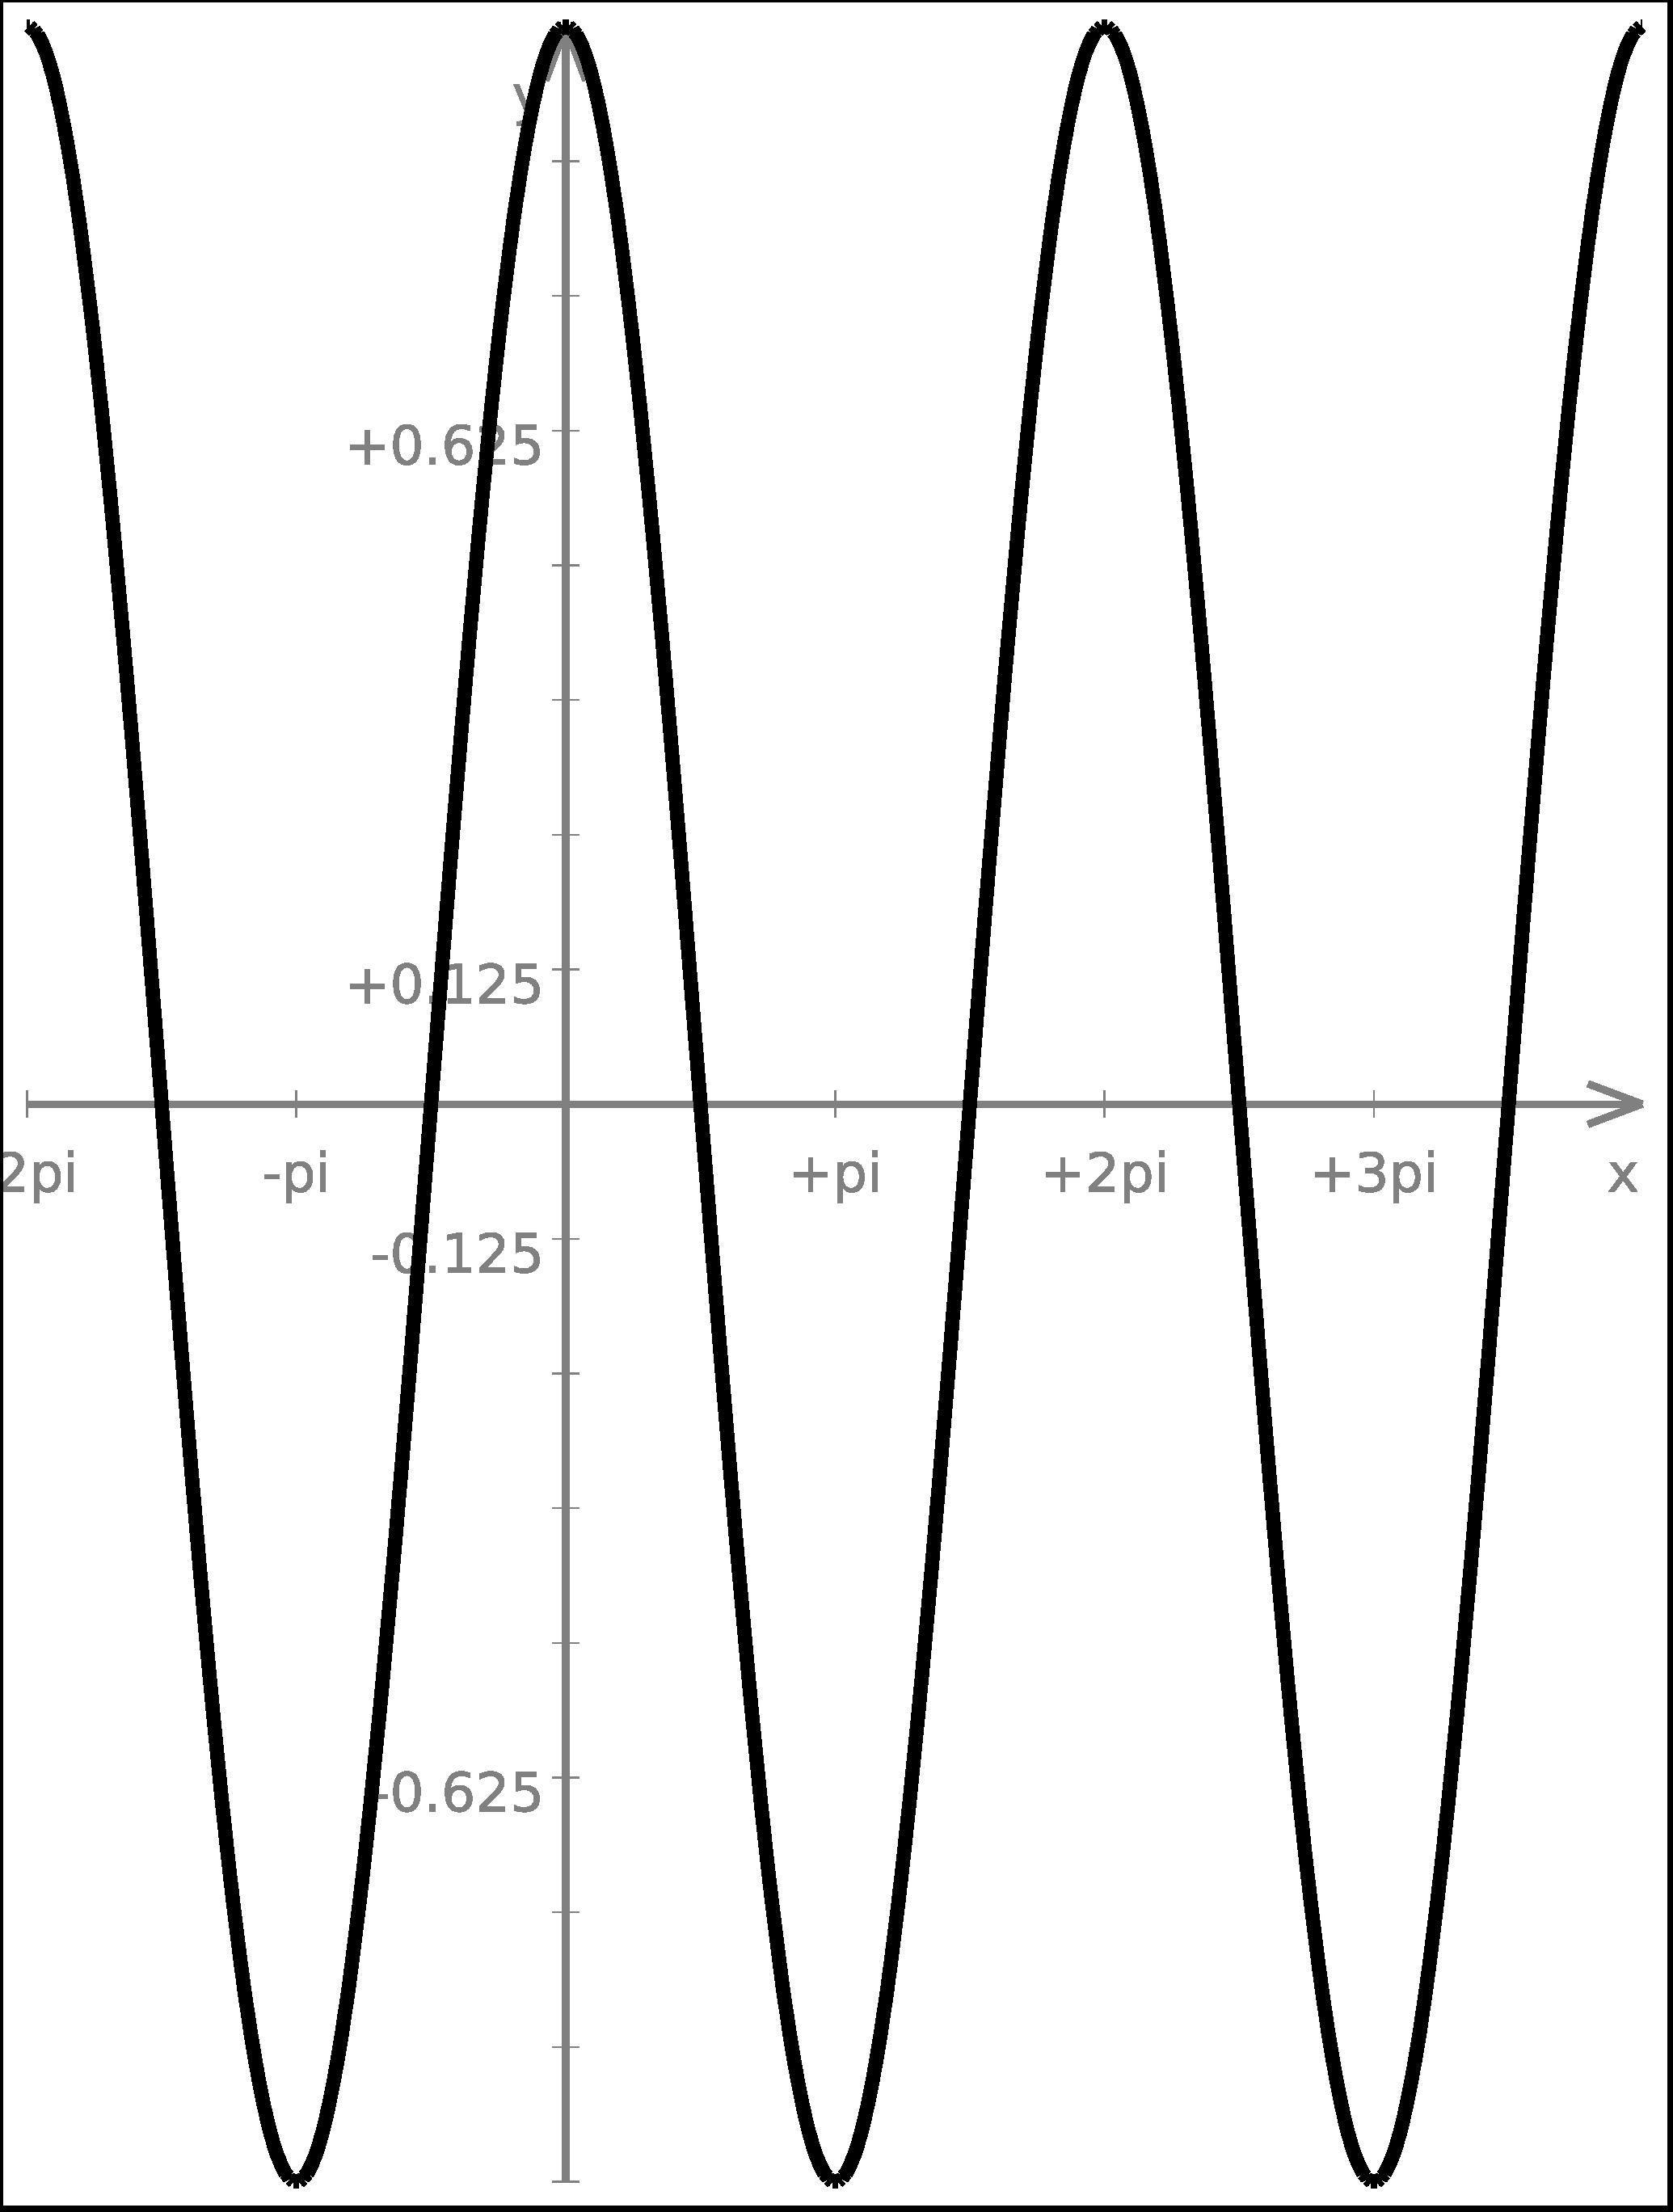
\includegraphics[width=\textwidth, height=2.5cm]{img/cos.pdf}
 $\cos x$ \end{center}
\end{minipage}\hfill
\begin{minipage}{.25\textwidth}
 \begin{center}
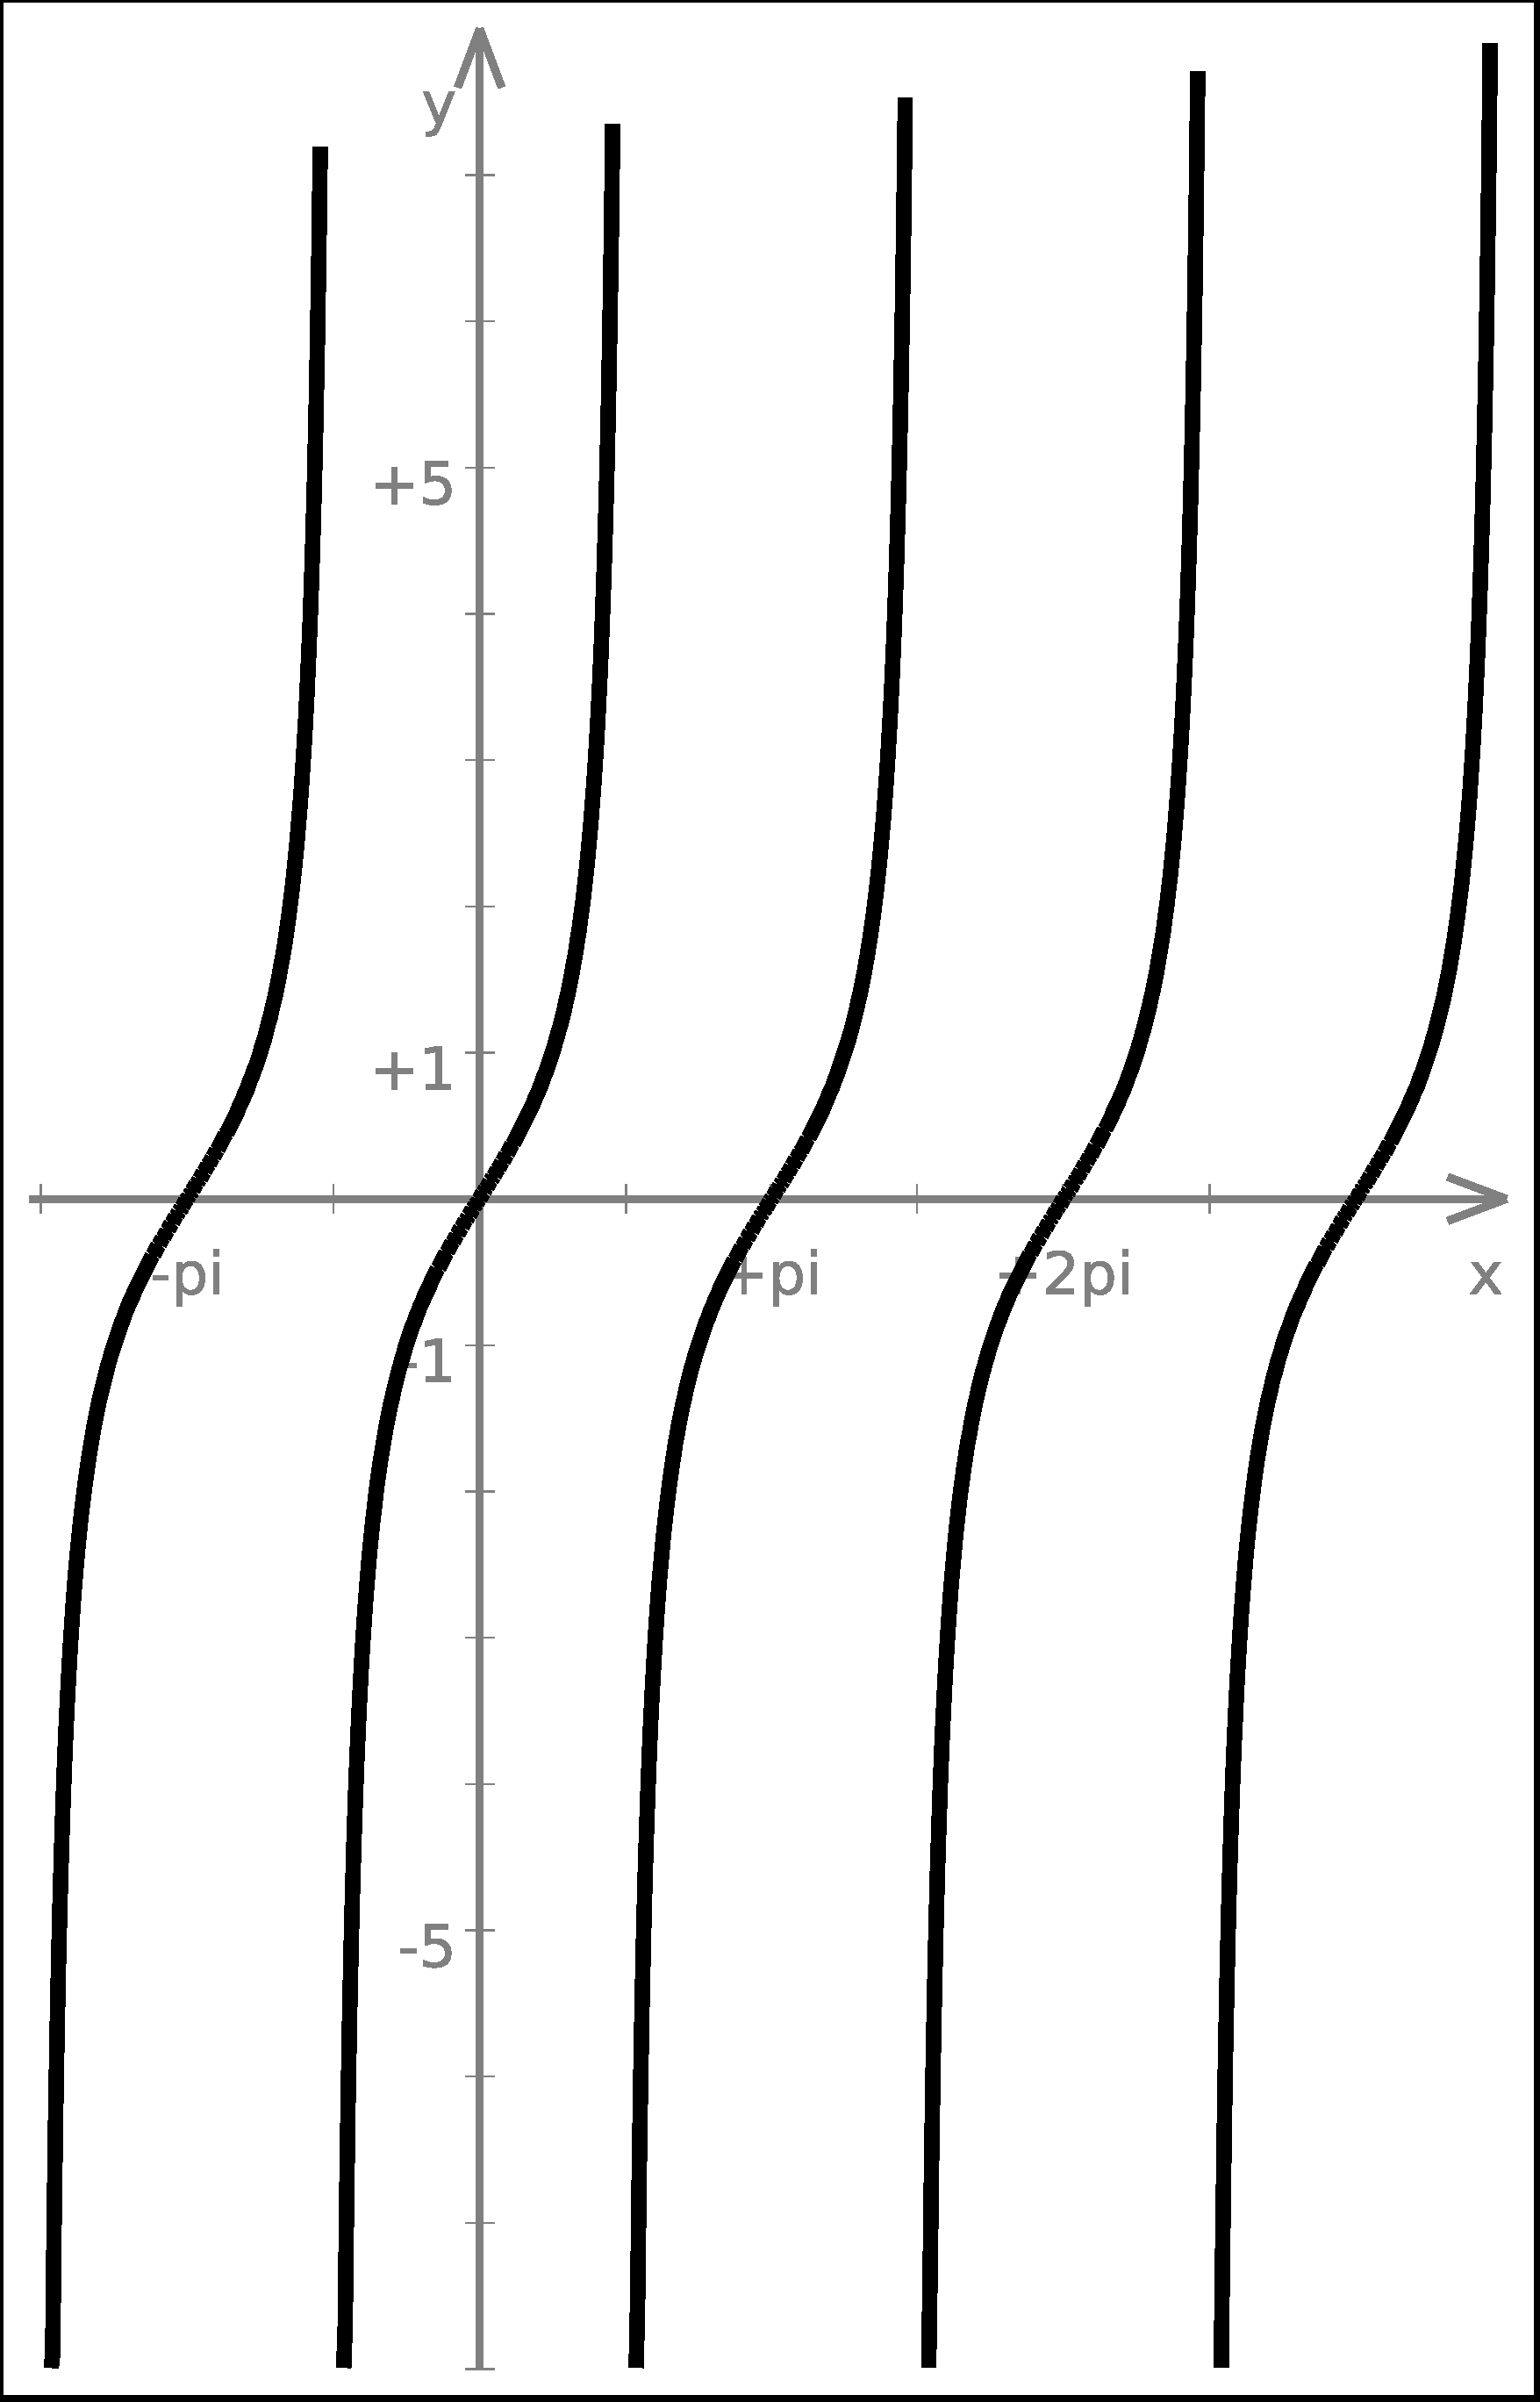
\includegraphics[width=\textwidth, height=4cm]{img/tan.pdf} 
 $\tan x$         \end{center}
\end{minipage}\hfill
%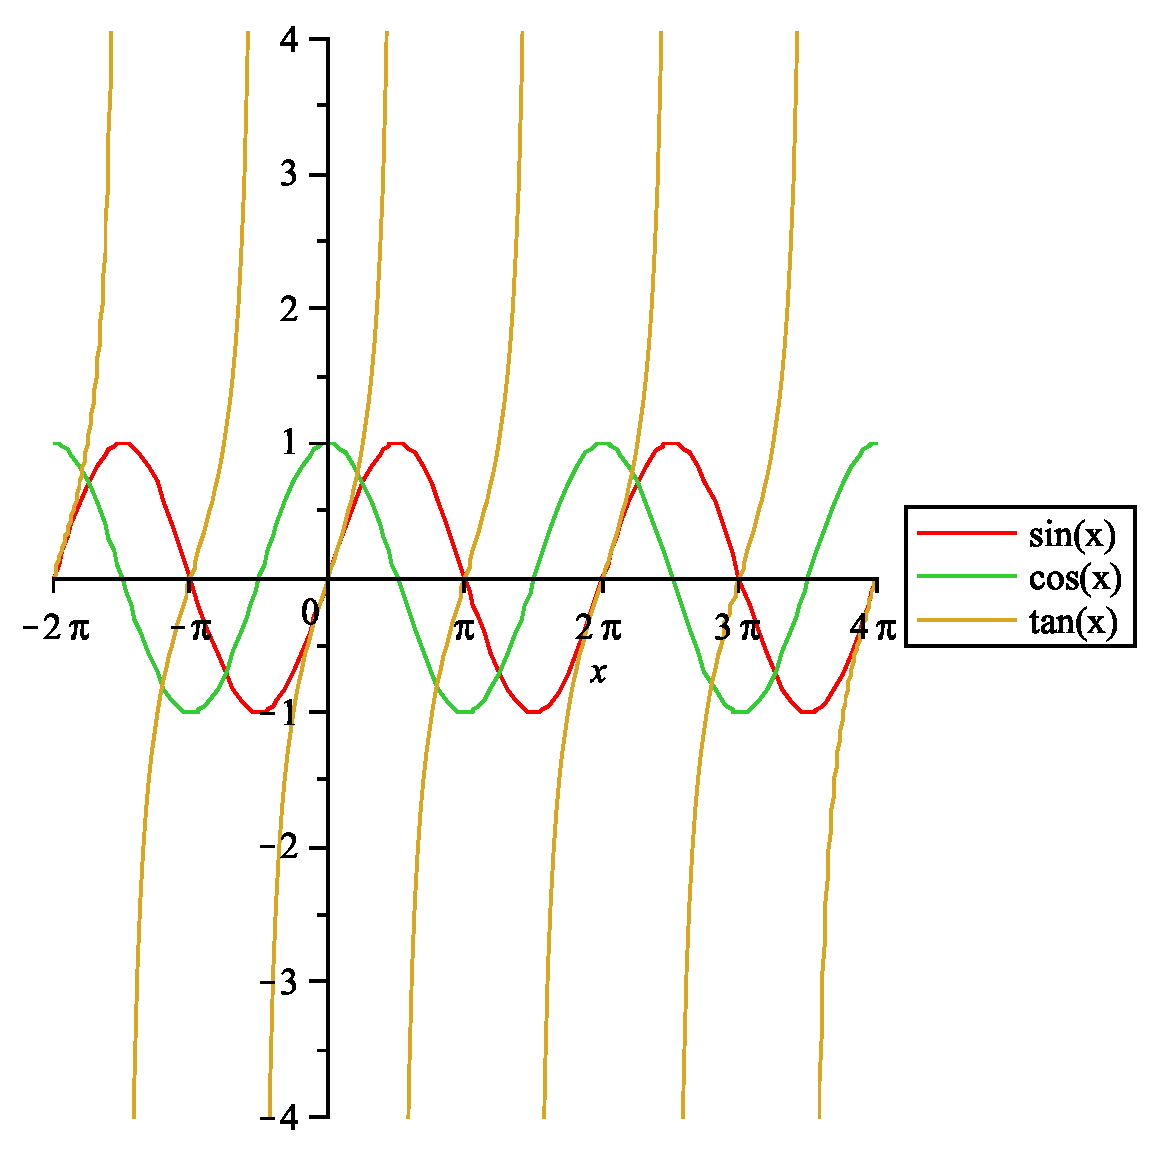
\includegraphics[height=8cm]{img/trig.pdf}
\end{center}

\noindent Man sieht, dass der Cosinus gegenüber dem Sinus nur um $\pitwo$
verschoben ist, es gilt also:
\[\sin \left( \pitwo-x \right) = \cos x \qquad
\cos \left( \pitwo-x\right) = \sin x\]

Beispiel:
\begin{gather*}
\cos\left(\pitwo\right) = \sin\left(\pitwo - \pitwo \right)= \sin(0) = 0\\
\displaybreak[0]
\sin\left(\frac{3\pi}{2} \right) = \cos\left(\pitwo - \frac{3\pi}{2} \right)
= \cos(-\pi) = -1
\end{gather*}

\subsection{Periodizität und Symmetrie}\label{sec:trig:perioden}
Alle Winkelfunktionen sind periodisch, d.~h. alle Werte wiederholen sich in
regelmäßigen Abständen. Es gilt also für jede ganze Zahl $k$:
\[\sin(x+2k\pi) = \sin x \quad \cos(x+2k\pi) = \cos x \quad \tan(x+k\pi) =
\tan x\] (Zur Erinnerung: $2\pi \equiv 360^\circ$, deswegen entspricht $2k\pi$ genau $k$ Vollkreisen).

\newpar
Beispiele:
\begin{gather*}
\sin\left(\pitwo\right) = \sin\left(\frac{5\pi}{2} \right)=
\sin\left(\frac{9\pi}{2} \right)= \sin\left(\frac{13\pi}{2} \right) = \dots\\
\cos(\pi) = \cos(3\pi) = \cos(5\pi) = \cos(7\pi) = \dots\\
\tan\left(\frac{\pi}{4}\right) = \tan\left(\frac{3\pi}{4}\right) =
\tan\left(\frac{5\pi}{4}\right) = \tan\left(\frac{5\pi}{4}\right) = \dots
\end{gather*}

\newpar

\noindent Die Sinus- und Cosinusfunktion sind symmetrisch, der Sinus ist
punktsymmetrisch zum Ursprung, der Cosinus achsensymmetrisch zur $y$-Achse.
Zusammen mit der Periodizität folgen daraus folgende Beziehungen:

\begin{align*}
\text{\scriptsize(2) } \sin(\pi-x)&= \phantom{-}\sin x& \cos(\pi-x)&=-\cos x &
\tan(\pi-x)
&= -\tan x\\
\text{\scriptsize(3) }\sin(\pi+x)&= -\sin x & \cos(\pi+x)&=-\cos x &
\tan(\pi+x)
&= \phantom{-}\tan x\\
\text{\scriptsize(4) } \sin(2\pi-x)&= -\sin x& \cos(2\pi-x)&=\phantom{-}\cos x
& \tan(2\pi-x)
&= -\tan x\\
\end{align*}

\noindent Das Vorzeichen ist also vom Quadranten abhängig, in dem sich $x$ befindet.
Diesen Zusammenhang zeigt Abbildung 7.2.

%\begin{center}
% 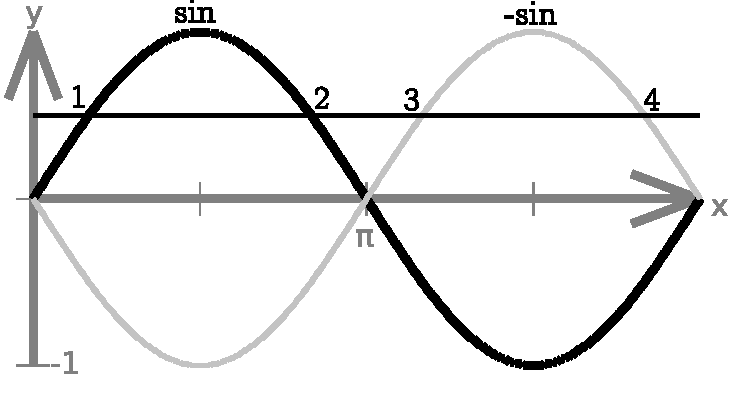
\includegraphics[width=.4\textwidth]{img/sin_sym.pdf}
%\end{center}
\begin{figure}[hbt]
\noindent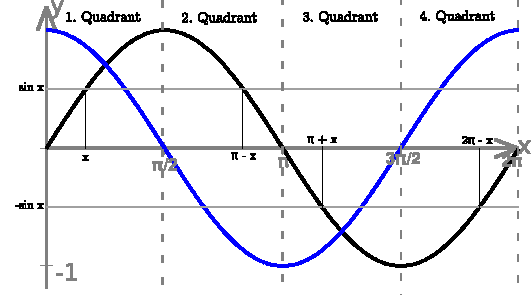
\includegraphics{img/symmetrie.pdf}

\vspace{-.15cm}
\hspace{.68cm}
\begin{tabular}{|p{1.56cm}|p{1.6cm}|p{1.6cm}|p{1.55cm}|}
 $\sin x$ & $+\sin x$ & $-\sin x$ & $-\sin x$\\
 $\cos x$ & $-\cos x$ & $-\cos x$ & $+\cos x$\\
 $\tan x$ & $-\tan x$ & $+\tan x$ & $-\tan x$\\
\hline
\end{tabular}
\label{fig:symmetrie}
\caption{Symmetrie von Sinus und Cosinus}
\end{figure}

\noindent Die Werte für $\sin x, 0 \leq x \leq \pitwo$ reichen damit aus, um alle
Werte für $\sin$ und $\cos$ bestimmen. Die wichtigsten Werte sind in der
folgenden Tabelle.
\[\begin{array}{|r|ccccc|}\hline
 x \text{ im Bogenmaß} & 0 & \frac{\pi}{6} &
\frac{\pi}{4} & \frac{\pi}{3} &
\pitwo\\
 x \text{ im Gradmaß}  & 0 & 30^\circ & 45^\circ & 60^\circ & 90^\circ\\
 \sin x                & \frac{1}{2}\sqrt{0} & \frac{1}{2}\sqrt{1}
& \frac{1}{2}\sqrt{2} &\frac{1}{2}\sqrt{3} & \frac{1}{2}\sqrt{4}\\
 \cos x    & \frac{1}{2}\sqrt{4} & \frac{1}{2}\sqrt{3} & \frac{1}{2}\sqrt{2}
 & \frac{1}{2}\sqrt{1} & \frac{1}{2}\sqrt{0}\\\hline
\end{array}\]



\subsection{Umkehrfunktionen}%: $arcsin$, $arccos$, $arctan$}
Die Umkehrfunktionen zu $\sin$, $\cos$ und $\tan$ sind $\arcsin$, $\arccos$
und $\arctan$ (sprich: \emph{arcus sinus}, \emph{arcus cosinus} und
\emph{arcus tangens}). Da die trigonometrischen Funktionen periodisch sind
(z.~B. gilt $\sin(0) = \sin(2\pi)=0$), kann es keine eindeutige Umkehrfunktion
geben (in diesem Beispiel: ist $\arcsin(0)$ gleich $0$ oder $2\pi$?).
Deswegen sind die Funktionen nur auf einem bestimmten Bereich umkehrbar.
Diese Bereiche sind:
\begin{eqnarray*}
y = \sin x\quad -\pitwo \leq x \leq \pitwo &
\Longleftrightarrow &
x = \arcsin y \quad -1 \leq y \leq 1 \\
y = \cos x\quad \phantom{--}0 \leq x \leq \pi &
\Longleftrightarrow &
x = \arccos y \quad -1 \leq y \leq 1\\
y = \tan x\quad -\pitwo < x < \pitwo &
\Longleftrightarrow &
x = \arctan y \quad y\in \mathbb{R}
\end{eqnarray*}

\subsection{Trigonometrischer Pythagoras}
Für alle $x$ gilt: $\sin^2 x + \cos^2 x = 1$. Diese Aussage heißt auch
\emph{trigonometrischer Pythagoras}. Damit kann manchmal ein Term vereinfacht
werden.

\subsection{Additionstheoreme}
Die Winkelfunktionen haben unter anderem diese wichtigen Eigenschaften:
\begin{eqnarray*}
 \sin(x_1 + x_2) &=& \sin x_1 \cos x_2 + \cos x_1 \sin x_2\\
 \sin(x_1 - x_2) &=& \sin x_1 \cos x_2 - \cos x_1 \sin x_2\\
 \cos(x_1 + x_2) &=& \cos x_1 \cos x_2 - \sin x_1 \sin x_2\\
 \cos(x_1 - x_2) &=& \cos x_1 \cos x_2 + \sin x_1 \sin x_2\\
\end{eqnarray*}

Beispiele:
\begin{align*}
 \sin(120^\circ) &= \sin(60^\circ +60^\circ) =
\sin(\tfrac{\pi}{3}+\tfrac{\pi}{3}) &\text{\scriptsize(wende
Additionstheorem an)}\\\displaybreak[0]
  &= \sin\tfrac{\pi}{3}\cos\tfrac{\pi}{3} +
\cos\tfrac{\pi}{3}\sin\tfrac{\pi}{3}\\
  &= \tfrac{1}{2}\sqrt{3}\cos\tfrac{\pi}{3}
+ \cos\left(\tfrac{\pi}{3}\right)\tfrac{1}{2}\sqrt{3} = \sqrt{3}
\smash{\cos\tfrac{\pi}{3}} &\text{\scriptsize (wandele $\cos$ in $\sin$)}\\
 &= \sqrt{3}\sin\left(\tfrac{\pi}{2} - \tfrac{\pi}{3} \right) =
\sqrt{3}\sin\tfrac{\pi}{6}\\
 &= \tfrac{1}{2}\sqrt{3}
\end{align*}
Probe über Symmetrie:
\begin{align*}
\sin(120^\circ) &= \sin\left(\tfrac{2\pi}{3} \right)
    = \sin(\pi-\tfrac{\pi}{3}) \quad\text{\scriptsize (mit
\ref{sec:trig:perioden}(2)) } \\
  &= \sin(\tfrac{\pi}{3})= \tfrac{1}{2}\sqrt{3}
\end{align*}

\subsection{Aufgaben}

\begin{enumerate}
 \item Berechne mit Hilfe der Tabelle in Abschnitt~\ref{sec:trig:perioden}
folgende Werte:
 \begin{multicols}{4}
  \begin{enumerate}
   \item $\sin \frac{2\pi}{3}$ 
   \item $\sin \frac{5\pi}{6}$
   \item $\sin \pi$
   \item $\sin \frac{3\pi}{2}$
   \item $\sin \frac{11\pi}{6}$
   \item $\sin \frac{7\pi}{3}$
   \item $\sin \frac{29\pi}{6}$
   \item $\sin -\frac{3\pi}{4}$
   \item $\cos \frac{\pi}{6}$
   \item $\cos \frac{\pi}{4}$
   \item $\cos \frac{\pi}{3}$
   \item $\cos \frac{\pi}{2}$
   \item $\cos \frac{11\pi}{6}$
   \item $\cos \frac{3\pi}{4}$
   \item $\cos \frac{2\pi}{3}$
   \item $\cos \frac{4\pi}{6}$
   \item $\cos \frac{7\pi}{3}$
   \item $\cos -\frac{11\pi}{4}$
   \item $\tan \frac{\pi}{6}$
   \item $\tan -\frac{\pi}{3}$
  \end{enumerate}
 \end{multicols}

\item Berechne die fehlenden Seitenlängen. Die
Bezeichnungen entsprechen der nebenstehenden Zeichnung.

\begin{minipage}{6cm}
\begin{tabular}{|ccccc|}
$\alpha$ & $\beta$ & $a$ & $b$ & $c$\\
\hline
& &  & $1$ & $\sqrt{2}$\\
& & 2 &  & 4\\ % b = $\sqrt{12}$
& & $\frac{1}{2}\sqrt{3}$& & $\frac{1}{2}$\\
& & 4 & 3 & \\
$\frac{\pi}{6}$ & & 1 & &\\
&$\frac{\pi}{3}$ & & 2 &\\
\end{tabular}
\end{minipage}
\begin{minipage}{4cm}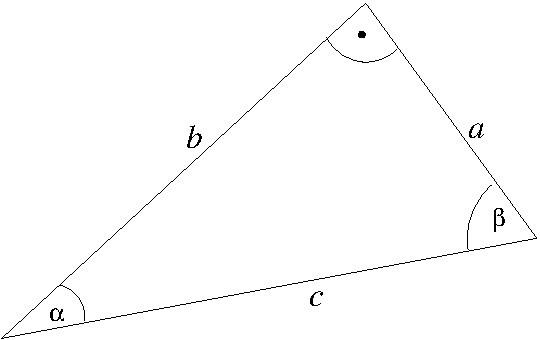
\includegraphics[width=4cm]{img/winkel_aufgaben.pdf}
\end{minipage}




 \item Leite folgende Aussage her: \[ \sin(4\alpha) = 4(\sin\alpha
\cdot \cos^3\alpha - \sin^3\alpha\cdot \cos\alpha)\]
 \item Leite her, dass folgende Aussage gilt:
\[\cos(2\alpha) = 2\cdot\cos^2\alpha -1 \]
 \item* Eine Kugel mit dem Radius 1 umschließt einen Würfel. Bestimme die
maximale Seitenlänge des Würfels.
\end{enumerate}

%%%weiter siehe log_e.tex

%\newcommand{\pitwo}{\frac{\pi}{2}}
\newcommand{\newpar}{\vspace{1em}\noindent}

\chapter{Funktionen}
\label{chap:funktionen}

Autor: Gerhard Gossen

\mbox{}\par
\section{Definition}
\noindent Eine Funktion $f$ ist eine Abbildung, die einem Wert aus dem \emph{Definitionsbereich $D(f)$} genau einen Wert aus dem \emph{Wertebereich $W(f)$} zuordnet. Die übliche Darstellung ist
$f : X \to Y$ (sprich: $f$ ist eine Abbildung von $X$ nach $Y$), wobei $X$ die Definitionsmenge ($D(f) \subseteq X$) und $Y$ die Zielmenge ist ($W(f) \subseteq Y$). Definitions- und Zielmenge sind oft $\R$ (die reellen Zahlen).

Verbreitete Funktionen sind z.B. Geraden ($f(x) = m\cdot x +n$), Polynome ($f(x) = a_n x^n + a_{n-1} x^{n-1}+\dots + a_1x+a_0$), die trigonometrischen Funktionen ($\sin x$, $\cos x$, $\tan x$, siehe Abschnitt~\ref{sec:trigonometrie}) oder Exponentialfunktionen ($a^x$, siehe Abschnitt~\ref{sec:exponential}). Abbildung~\ref{fig:funktionen} zeigt die Graphen einiger Funktionen.

\begin{figure}[bth]
\begin{center}
    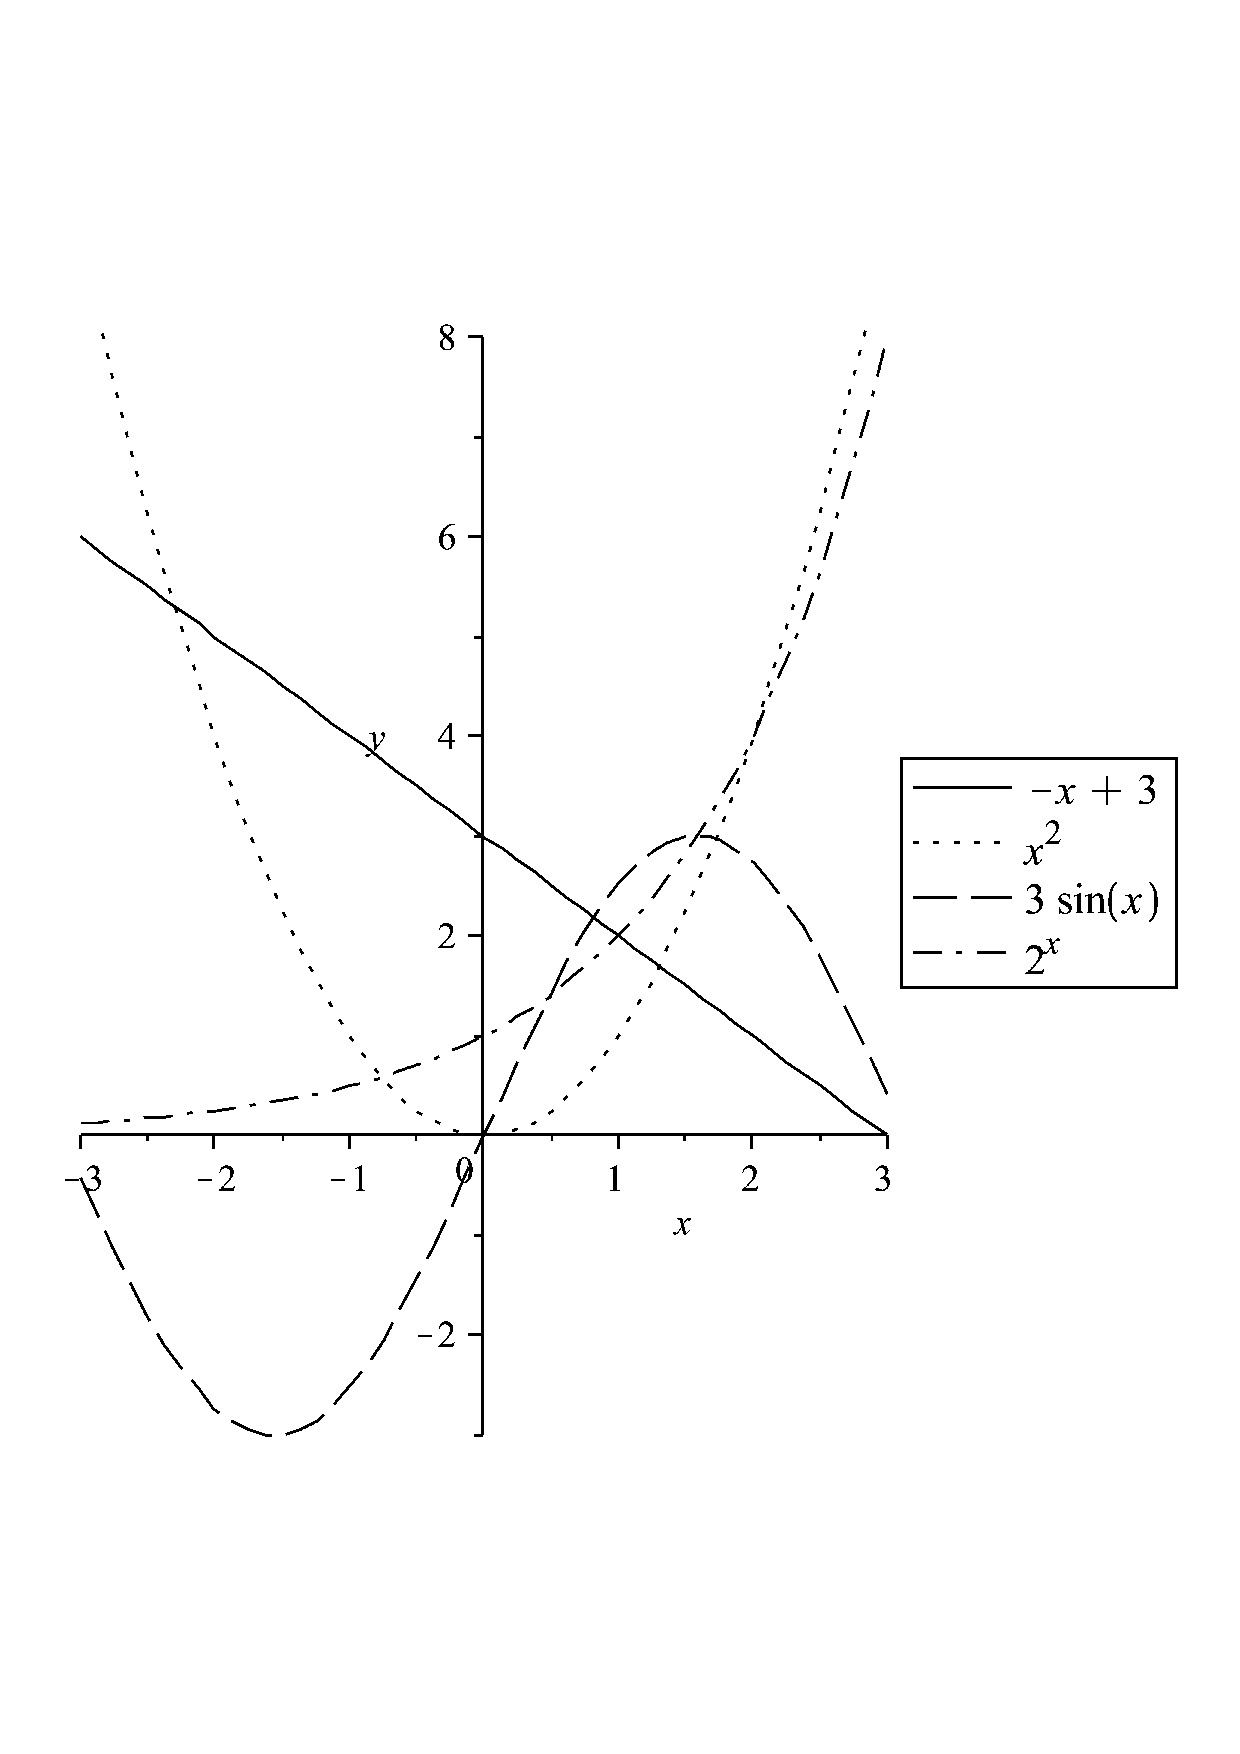
\includegraphics[width=0.5\textwidth]{img/Funktionssammlung.}
\end{center}
\caption{Bekannte Funktionen}
\label{fig:funktionen}
\end{figure} 

Alle Funktionen, die wir im Vorkurs behandeln, sind Funktionen mit \emph{einer Ver"-änderlichen}, also Funktionen, die von einer einzigen Variable (meist $x$) ab"-hän"-gen. % In der Vorlesung werden Funktionen mit \emph{mehreren Veränderlichen} behandelt.

Die Eigenschaften einer Funktion kann man über eine \emph{Kurvendiskussion} (siehe Abschnitt~\ref{sec:kurvendiskussion}) herausbekommen. Zuerst werden wir aber zwei wichtige Funktionsfamilien vorstellen: die trigonometrischen Funktionen (Winkelfunktionen, Abschnitt~\ref{sec:trigonometrie}) und die Exponentialfunktionen (Abschnitt~\ref{sec:exponential}).

%%%%%%%%%%%%%%%%%%%%%%%%%%%%%%%%%%%%%%%%%%%%%%%%%%%%%%%%%%%%%%%%%%%%%%%%%%%%%%%%%%%%%%5
\section{Trigonometrische Funktionen%: $sin$, $cos$, $tan$
}\label{sec:trigonometrie}

Die trigonometrischen Funktionen $\sin, \cos, \tan$ sind die
Winkelfunktionen. Sie sind für Winkel im Bogenmaß definiert (z.\,B. $ x =
\pitwo$). Winkel im Gradmaß (z.\,B. $ x = 90^\circ$) können
eindeutig ins Bogenmaß umgerechnet werden ($90^\circ \equiv \pitwo$).
Deswegen ist auch die Schreibweise $\sin 90^\circ$ möglich.

\subsection{Definition}
Im rechtwinkligen Dreieck gilt:

\begin{minipage}{.5\linewidth}
\begin{eqnarray*}
 \sin x &=& \frac{\text{Gegenkathete}}{\text{Hypothenuse}}\\
 \cos x &=& \frac{\text{Ankathete}}{\text{Hypothenuse}}\\
 \tan x &=& \frac{\text{Gegenkathete}}{\text{Ankathete}} =
\frac{\sin x}{\cos x}
\end{eqnarray*}
\end{minipage}\hspace{.1\linewidth}
\begin{minipage}{.35\textwidth}
 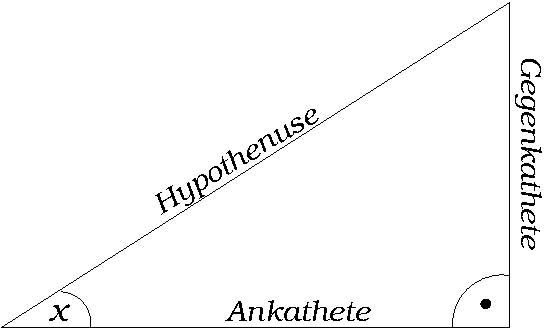
\includegraphics[width=\textwidth]{img/winkel.pdf}
%\vspace{.1em}
\end{minipage}

Diese Definitionen lassen sich verallgemeinern, so dass die Funktionen für 
alle reelen Zahlen definiert sind (im rechtwinkligen Dreieck:
$0\leq x \leq 90^\circ$). Damit ergeben sich diese Funktionen:
\begin{center}\hfill
\begin{minipage}{.25\textwidth}
 \begin{center}
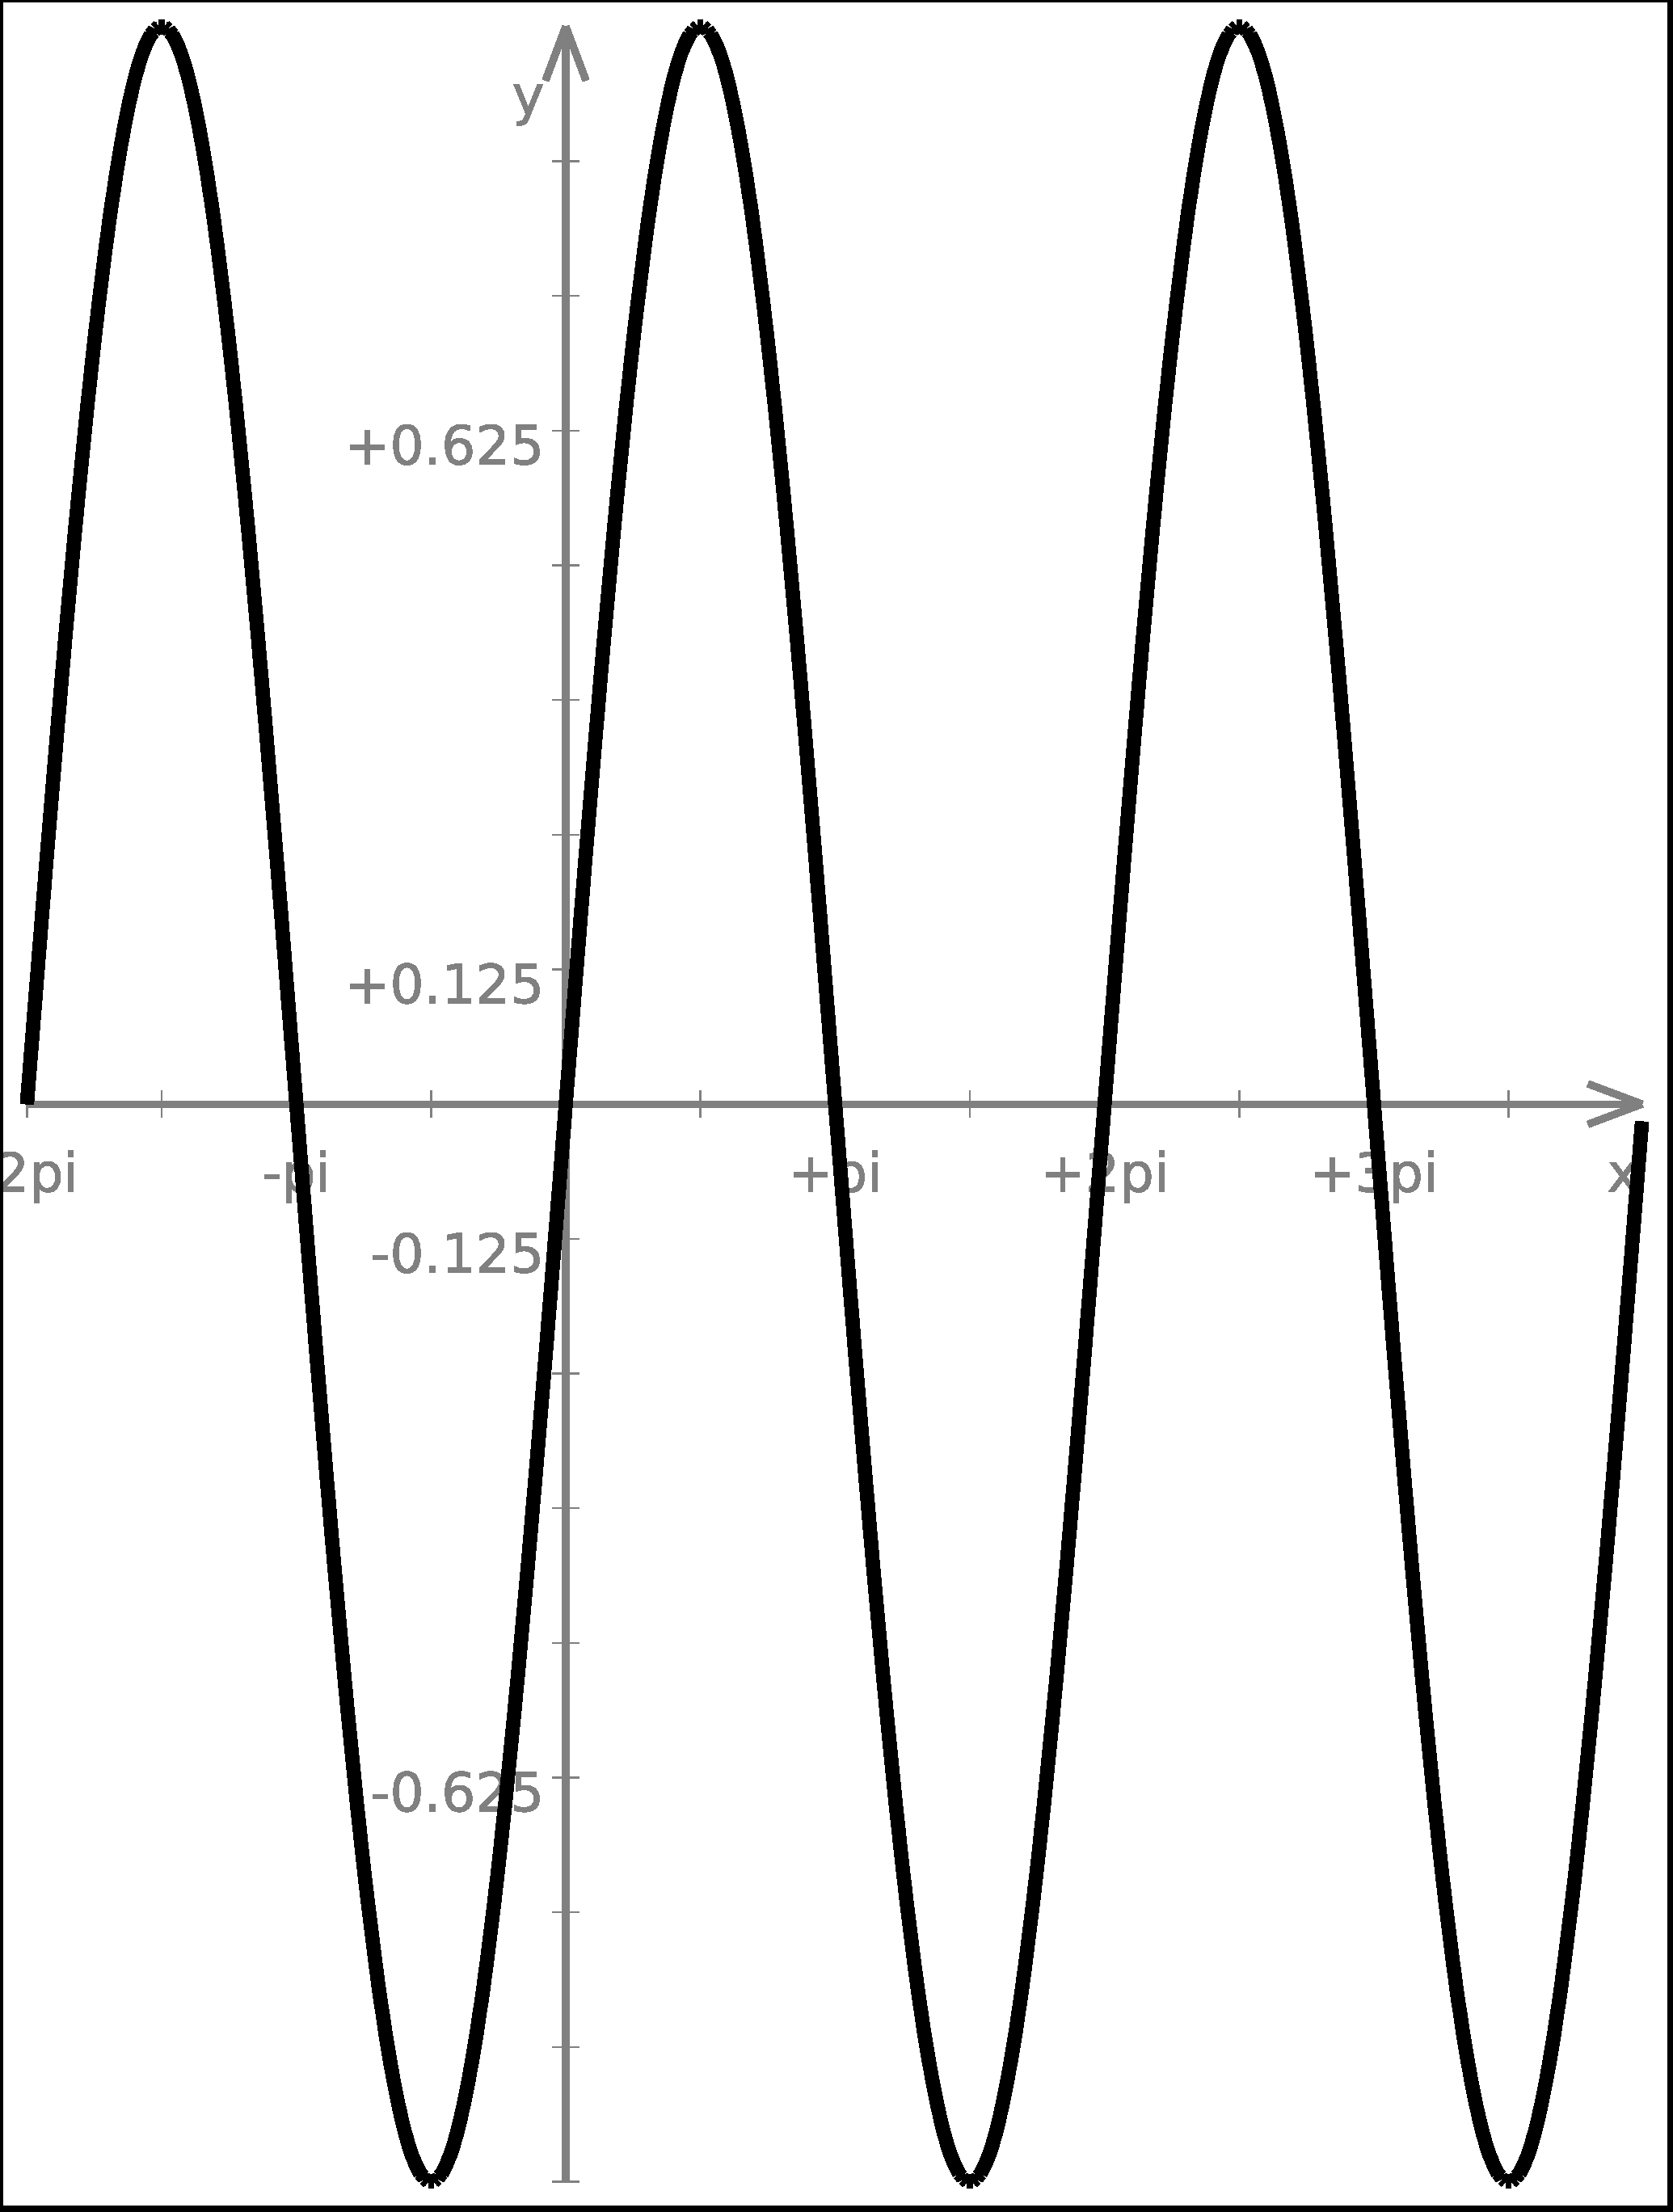
\includegraphics[width=\textwidth, height=2.5cm]{img/sin.pdf}
 $\sin x$         \end{center}
\end{minipage}\hfill
\begin{minipage}{.25\textwidth}
 \begin{center}
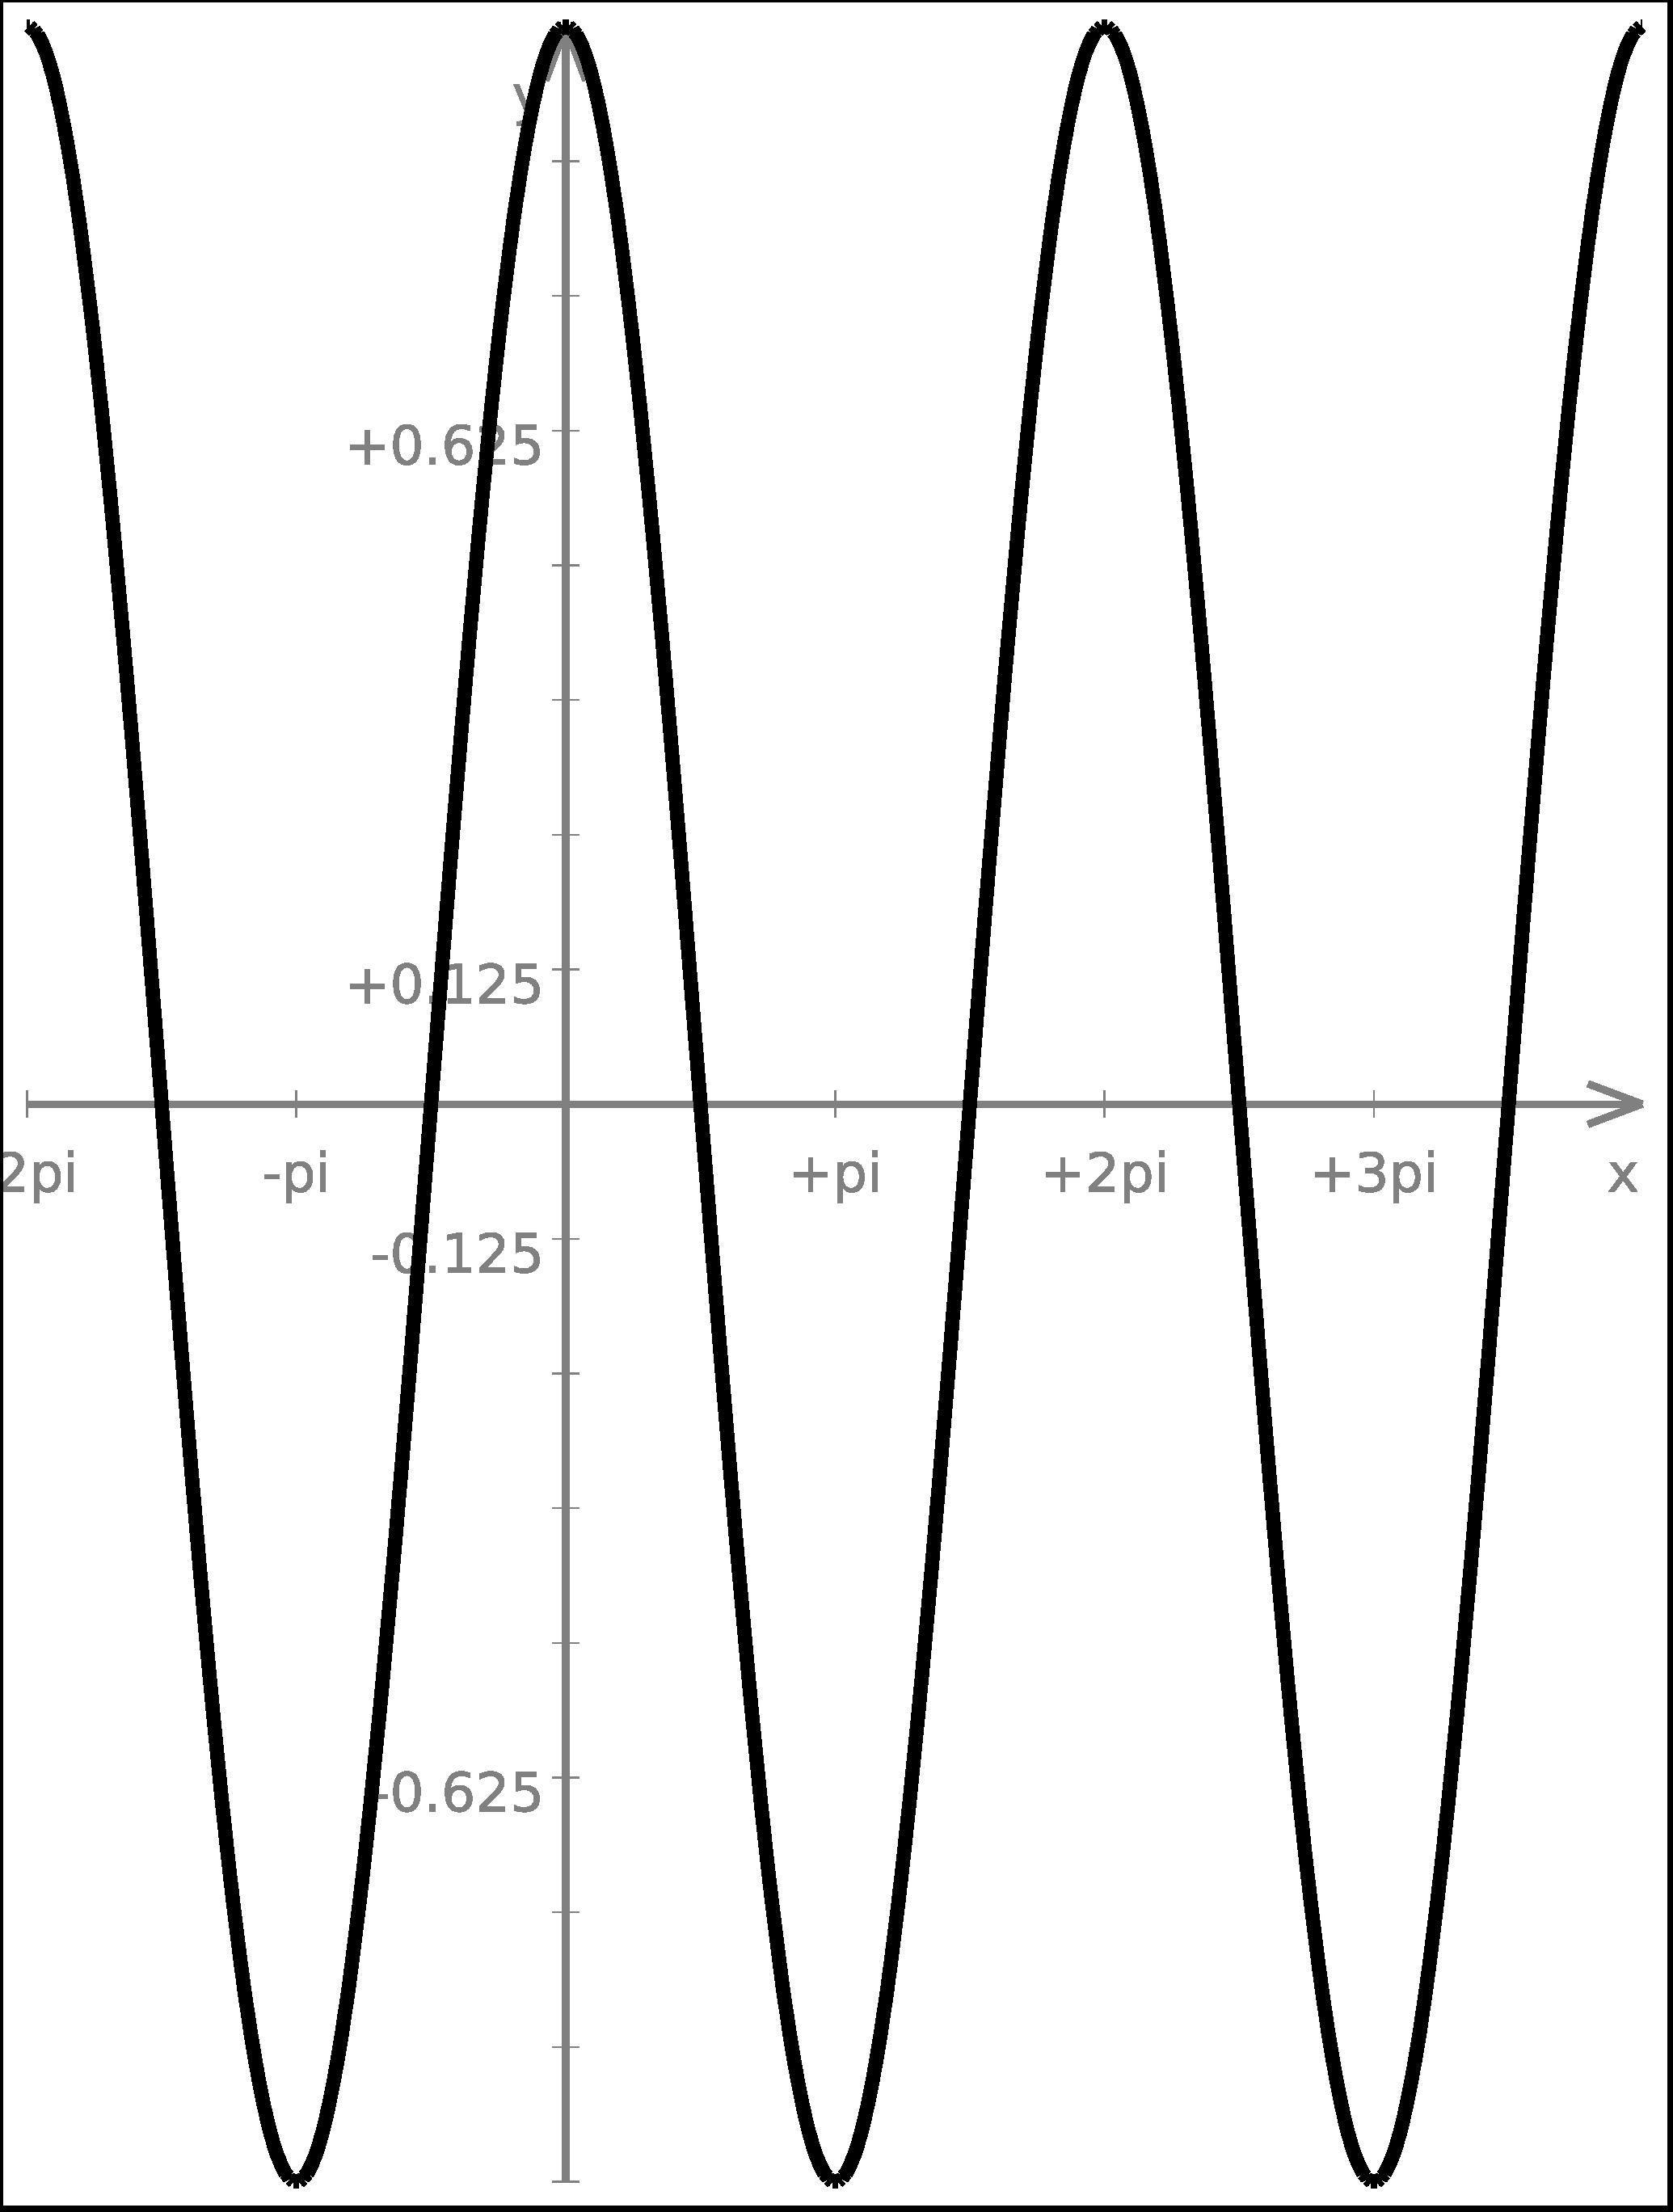
\includegraphics[width=\textwidth, height=2.5cm]{img/cos.pdf}
 $\cos x$ \end{center}
\end{minipage}\hfill
\begin{minipage}{.25\textwidth}
 \begin{center}
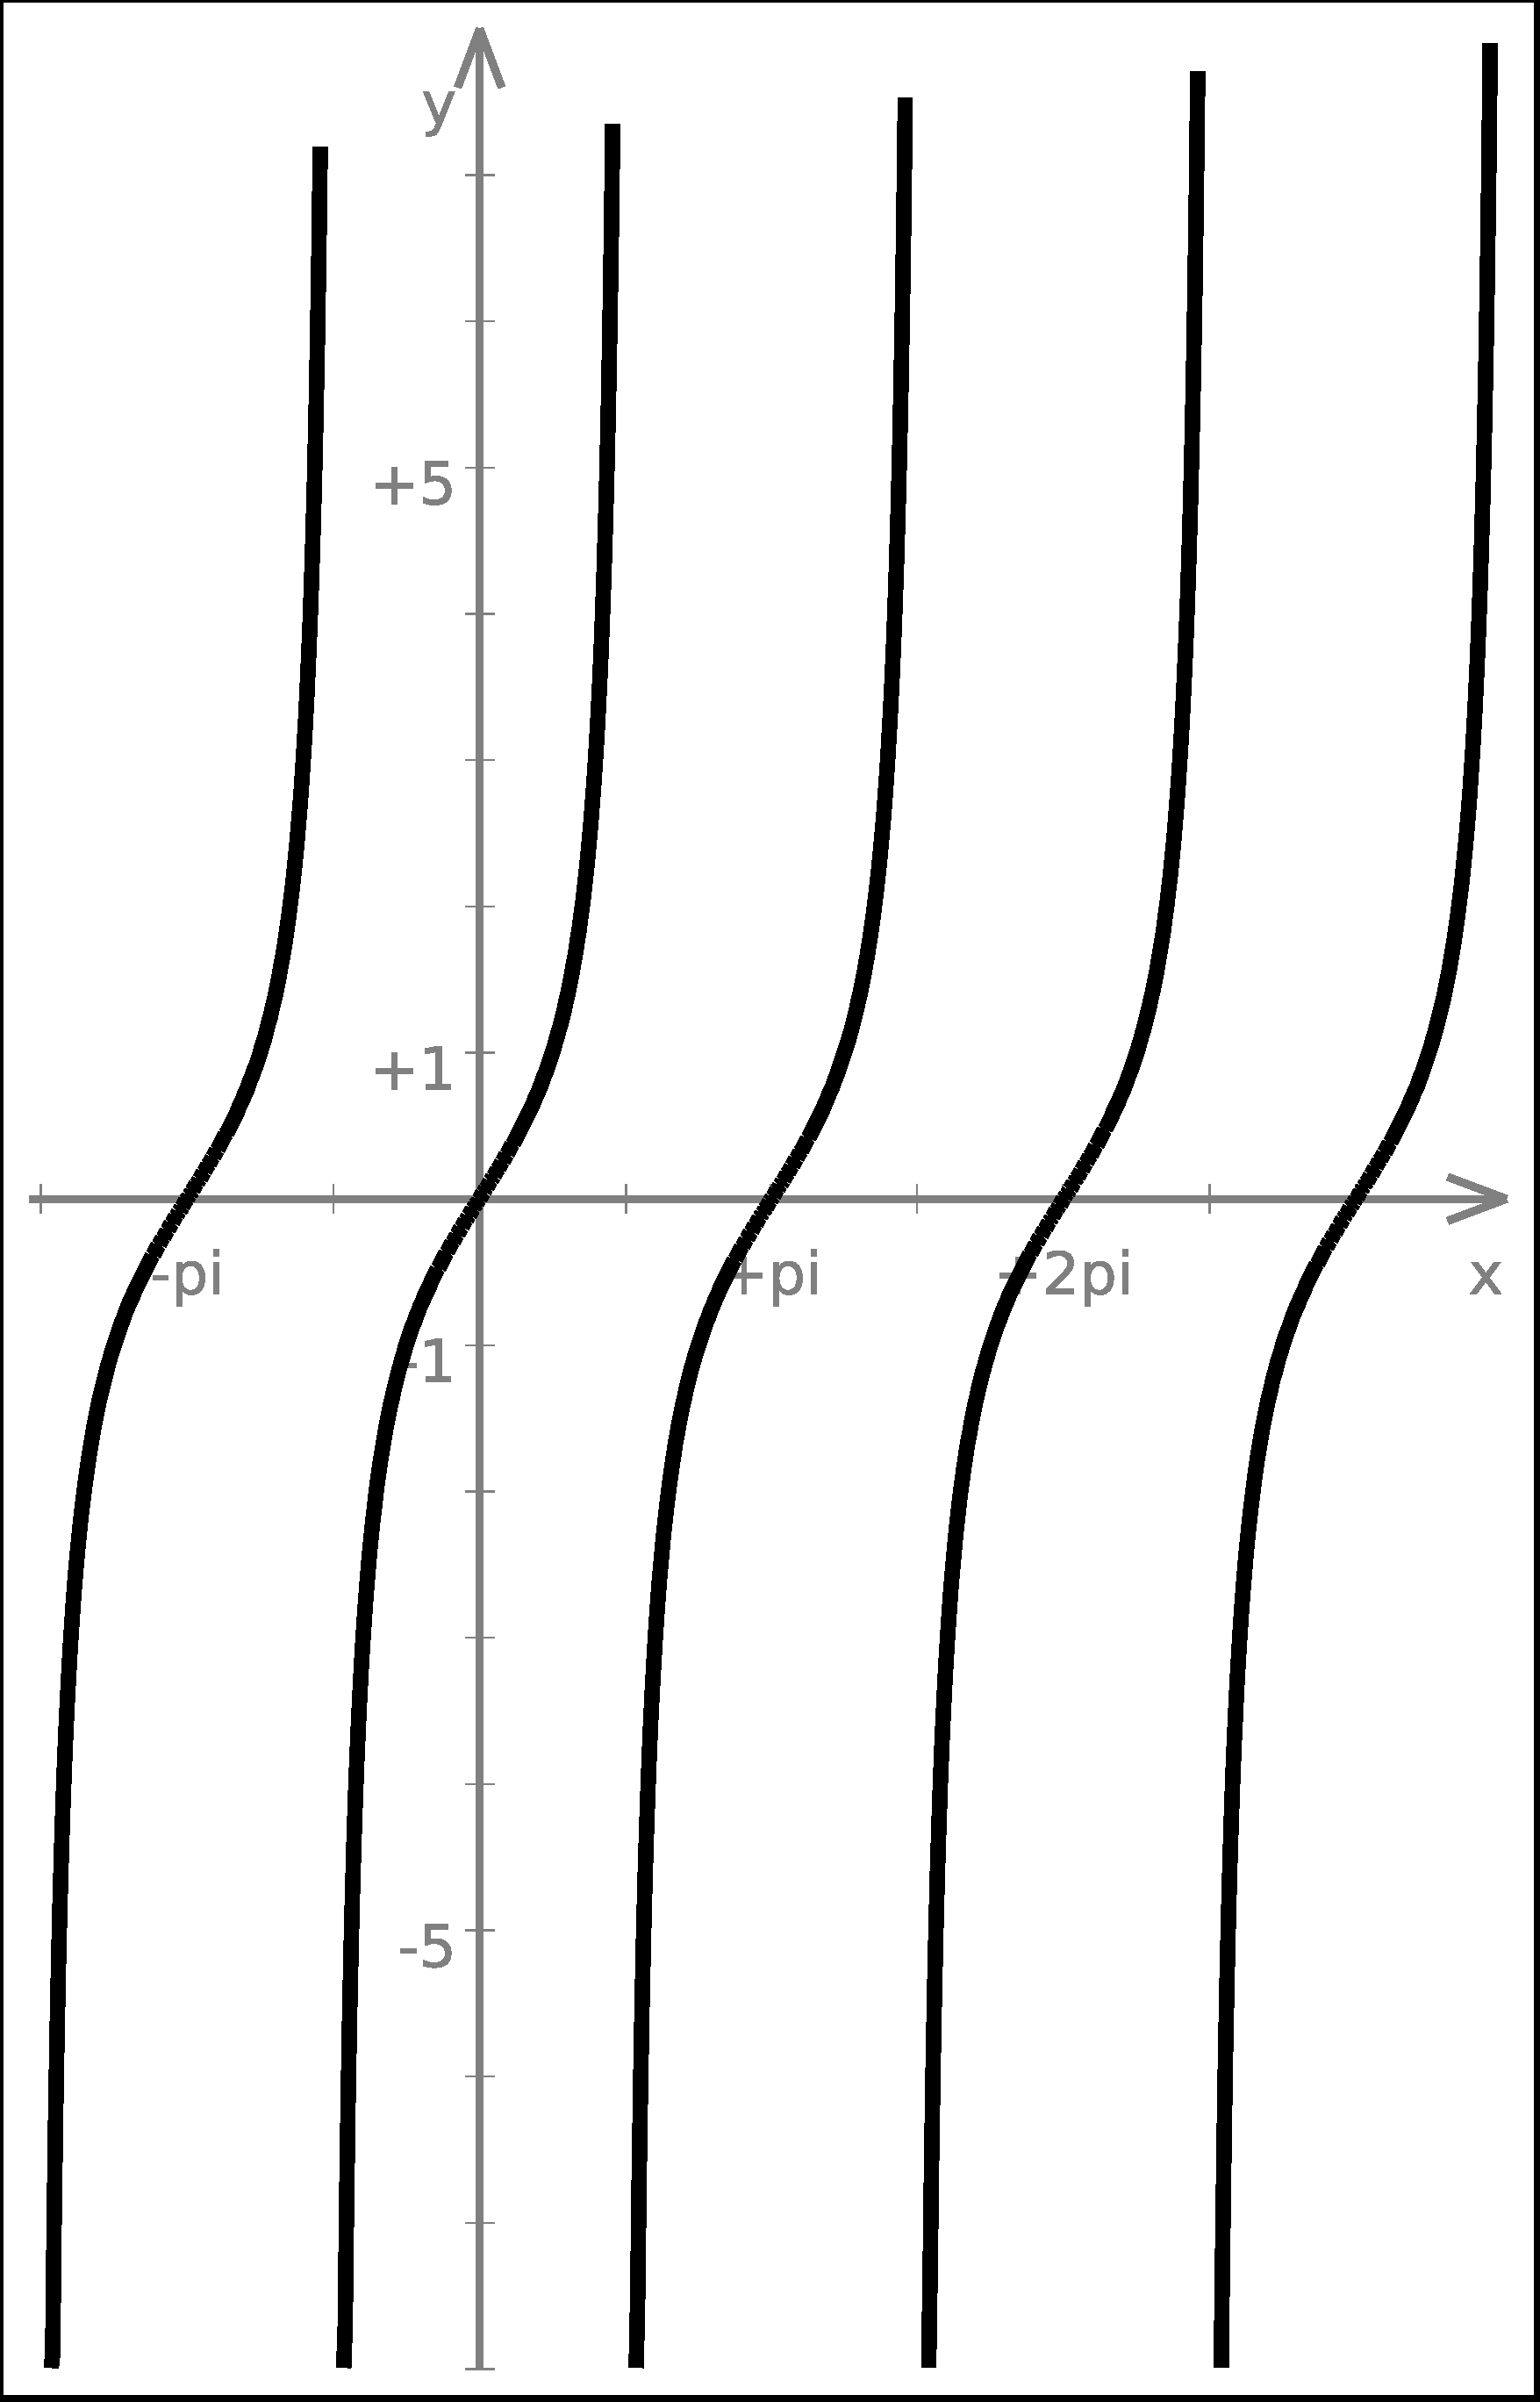
\includegraphics[width=\textwidth, height=4cm]{img/tan.pdf} 
 $\tan x$         \end{center}
\end{minipage}\hfill
%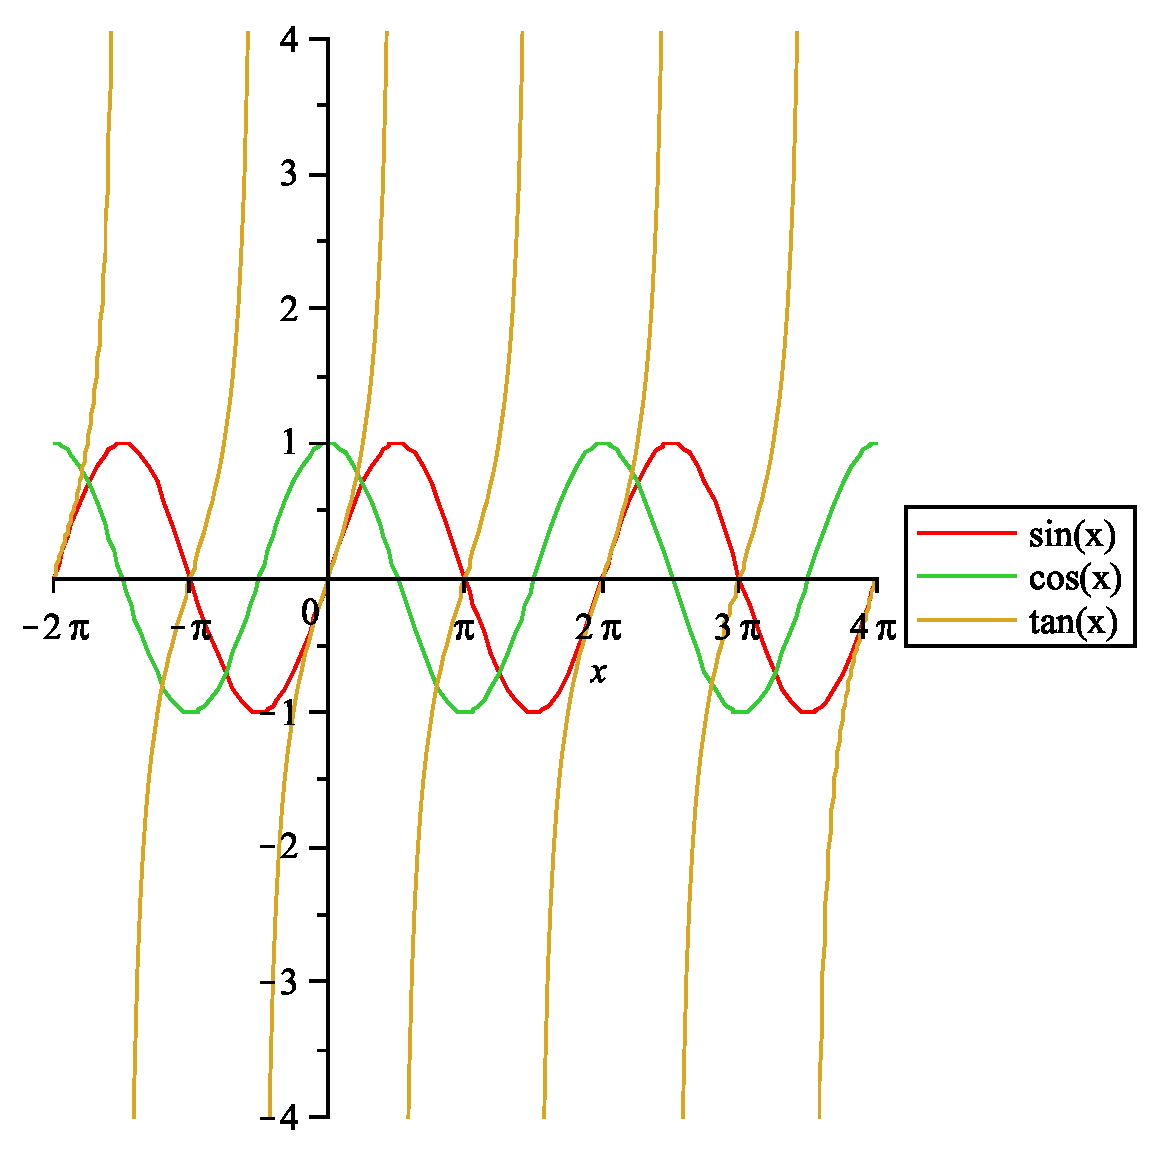
\includegraphics[height=8cm]{img/trig.pdf}
\end{center}

Man sieht, dass der Cosinus gegenüber dem Sinus nur um $\pitwo$
verschoben ist, es gilt also:
\[\sin \left( \pitwo-x \right) = \cos x \qquad
\cos \left( \pitwo-x\right) = \sin x\]

Beispiel:
\begin{gather*}
\cos\left(\pitwo\right) = \sin\left(\pitwo - \pitwo \right)= \sin(0) = 0\\
\displaybreak[0]
\sin\left(\frac{3\pi}{2} \right) = \cos\left(\pitwo - \frac{3\pi}{2} \right)
= \cos(-\pi) = -1
\end{gather*}

\subsection{Periodizität und Symmetrie}\label{sec:trig:perioden}
Alle Winkelfunktionen sind periodisch, d.~h. alle Werte wiederholen sich in
regelmäßigen Abständen. Es gilt also für jede ganze Zahl $k$:
\[\sin(x+2k\pi) = \sin x \quad \cos(x+2k\pi) = \cos x \quad \tan(x+k\pi) =
\tan x\] (Zur Erinnerung: $2\pi \equiv 360^\circ$, deswegen entspricht $2k\pi$ genau $k$ Vollkreisen).

\newpar
Beispiele:
\begin{gather*}
\sin\left(\pitwo\right) = \sin\left(\frac{5\pi}{2} \right)=
\sin\left(\frac{9\pi}{2} \right)= \sin\left(\frac{13\pi}{2} \right) = \dots\\
\cos(\pi) = \cos(3\pi) = \cos(5\pi) = \cos(7\pi) = \dots\\
\tan\left(\frac{\pi}{4}\right) = \tan\left(\frac{3\pi}{4}\right) =
\tan\left(\frac{5\pi}{4}\right) = \tan\left(\frac{5\pi}{4}\right) = \dots
\end{gather*}

\newpar

Die Sinus- und Cosinusfunktion sind symmetrisch, der Sinus ist
punktsymmetrisch zum Ursprung, der Cosinus achsensymmetrisch zur $y$-Achse.
Zusammen mit der Periodizität folgen daraus folgende Beziehungen:

\begin{align*}
\text{\scriptsize(2) } \sin(\pi-x)&= \phantom{-}\sin x& \cos(\pi-x)&=-\cos x &
\tan(\pi-x)
&= -\tan x\\
\text{\scriptsize(3) }\sin(\pi+x)&= -\sin x & \cos(\pi+x)&=-\cos x &
\tan(\pi+x)
&= \phantom{-}\tan x\\
\text{\scriptsize(4) } \sin(2\pi-x)&= -\sin x& \cos(2\pi-x)&=\phantom{-}\cos x
& \tan(2\pi-x)
&= -\tan x\\
\end{align*}

Das Vorzeichen ist also vom Quadranten abhängig, in dem sich $x$ befindet.
Diesen Zusammenhang zeigt Abbildung~\ref{fig:symmetrie}.

%\begin{center}
% 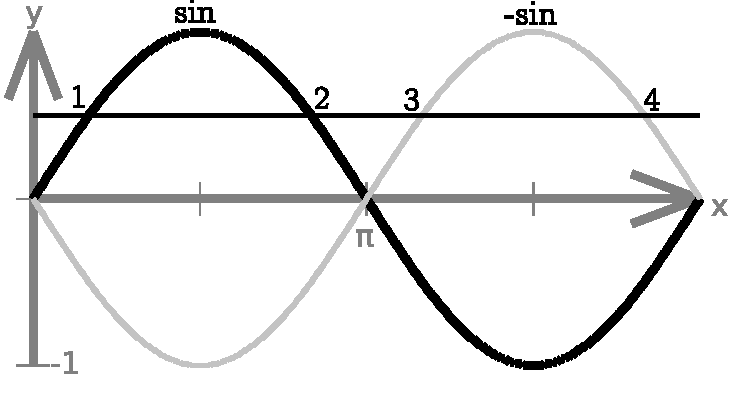
\includegraphics[width=.4\textwidth]{img/sin_sym.pdf}
%\end{center}
\begin{figure}[hbt]
\noindent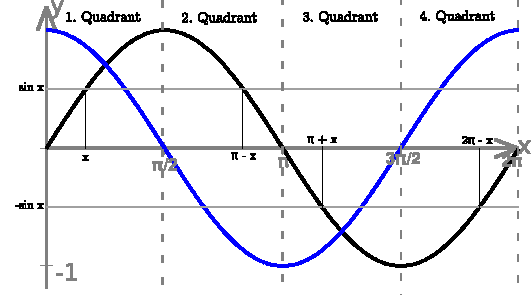
\includegraphics{img/symmetrie.pdf}

\vspace{-.15cm}
\hspace{.68cm}
\begin{tabular}{|p{1.56cm}|p{1.6cm}|p{1.6cm}|p{1.55cm}|}
 $\sin x$ & $+\sin x$ & $-\sin x$ & $-\sin x$\\
 $\cos x$ & $-\cos x$ & $-\cos x$ & $+\cos x$\\
 $\tan x$ & $-\tan x$ & $+\tan x$ & $-\tan x$\\
\hline
\end{tabular}
\label{fig:symmetrie}
\caption{Symmetrie von Sinus und Cosinus}
\end{figure}

Die Werte für $\sin x, 0 \leq x \leq \pitwo$ reichen damit aus, um alle
Werte für $\sin$ und $\cos$ bestimmen. Die wichtigsten Werte sind in der
folgenden Tabelle.
\[\begin{array}{|r|ccccc|}\hline
 x \text{ im Bogenmaß} & 0 & \frac{\pi}{6} &
\frac{\pi}{4} & \frac{\pi}{3} &
\pitwo\\
 x \text{ im Gradmaß}  & 0 & 30^\circ & 45^\circ & 60^\circ & 90^\circ\\
 \sin x                & \frac{1}{2}\sqrt{0} & \frac{1}{2}\sqrt{1}
& \frac{1}{2}\sqrt{2} &\frac{1}{2}\sqrt{3} & \frac{1}{2}\sqrt{4}\\
 \cos x    & \frac{1}{2}\sqrt{4} & \frac{1}{2}\sqrt{3} & \frac{1}{2}\sqrt{2}
 & \frac{1}{2}\sqrt{1} & \frac{1}{2}\sqrt{0}\\\hline
\end{array}\]



\subsection{Umkehrfunktionen}%: $arcsin$, $arccos$, $arctan$}
Die Umkehrfunktionen zu $\sin$, $\cos$ und $\tan$ sind $\arcsin$, $\arccos$
und $\arctan$ (sprich: \emph{arcus sinus}, \emph{arcus cosinus} und
\emph{arcus tangens}). Da die trigonometrischen Funktionen periodisch sind
(z.~B. gilt $\sin(0) = \sin(2\pi)=0$), kann es keine eindeutige Umkehrfunktion
geben (in diesem Beispiel: ist $\arcsin(0)$ gleich $0$ oder $2\pi$?).
Deswegen sind die Funktionen nur auf einem bestimmten Bereich umkehrbar.
Diese Bereiche sind:
\begin{eqnarray*}
y = \sin x\quad -\pitwo \leq x \leq \pitwo &
\Longleftrightarrow &
x = \arcsin y \quad -1 \leq y \leq 1 \\
y = \cos x\quad \phantom{--}0 \leq x \leq \pi &
\Longleftrightarrow &
x = \arccos y \quad -1 \leq y \leq 1\\
y = \tan x\quad -\pitwo < x < \pitwo &
\Longleftrightarrow &
x = \arctan y \quad y\in \mathbb{R}
\end{eqnarray*}

\subsection{Trigonometrischer Pythagoras}
Für alle $x$ gilt: $\sin^2 x + \cos^2 x = 1$. Diese Aussage heißt auch
\emph{trigonometrischer Pythagoras}. Damit kann manchmal ein Term vereinfacht
werden.

\subsection{Additionstheoreme}
Die Winkelfunktionen haben unter anderem diese wichtigen Eigenschaften:
\begin{eqnarray*}
 \sin(x_1 \pm x_2) &=& \sin x_1 \cos x_2 \pm \cos x_1 \sin x_2\\
 \cos(x_1 \pm x_2) &=& \cos x_1 \cos x_2 \mp \sin x_1 \sin x_2\\
\end{eqnarray*}

Beispiele:
\begin{align*}
 \sin(120^\circ) &= \sin(60^\circ +60^\circ) =
\sin(\tfrac{\pi}{3}+\tfrac{\pi}{3}) &\text{\scriptsize(wende
Additionstheorem an)}\\\displaybreak[0]
  &= \sin\tfrac{\pi}{3}\cos\tfrac{\pi}{3} +
\cos\tfrac{\pi}{3}\sin\tfrac{\pi}{3}\\
  &= \tfrac{1}{2}\sqrt{3}\cos\tfrac{\pi}{3}
+ \cos\left(\tfrac{\pi}{3}\right)\tfrac{1}{2}\sqrt{3} = \sqrt{3}
\smash{\cos\tfrac{\pi}{3}} &\text{\scriptsize (wandele $\cos$ in $\sin$)}\\
 &= \sqrt{3}\sin\left(\tfrac{\pi}{2} - \tfrac{\pi}{3} \right) =
\sqrt{3}\sin\tfrac{\pi}{6}\\
 &= \tfrac{1}{2}\sqrt{3}
\end{align*}
Probe über Symmetrie:
\begin{align*}
\sin(120^\circ) &= \sin\left(\tfrac{2\pi}{3} \right)
    = \sin(\pi-\tfrac{\pi}{3}) \quad\text{\scriptsize (mit
\ref{sec:trig:perioden}(2)) } \\
  &= \sin(\tfrac{\pi}{3})= \tfrac{1}{2}\sqrt{3}
\end{align*}

\subsection{Aufgaben}

\begin{enumerate}
 \item Berechne mit Hilfe der Tabelle in Abschnitt~\ref{sec:trig:perioden}
folgende Werte:
 \begin{multicols}{4}
  \begin{enumerate}
   \item $\sin \frac{2\pi}{3}$ 
   \item $\sin \frac{5\pi}{6}$
   \item $\sin \pi$
   \item $\sin \frac{3\pi}{2}$
   \item $\sin \frac{11\pi}{6}$
   \item $\sin \frac{7\pi}{3}$
   \item $\sin \frac{29\pi}{6}$
   \item $\sin -\frac{3\pi}{4}$
   \item $\cos \frac{\pi}{6}$
   \item $\cos \frac{\pi}{4}$
   \item $\cos \frac{\pi}{3}$
   \item $\cos \frac{\pi}{2}$
   \item $\cos \frac{11\pi}{6}$
   \item $\cos \frac{3\pi}{4}$
   \item $\cos \frac{2\pi}{3}$
   \item $\cos \frac{4\pi}{6}$
   \item $\cos \frac{7\pi}{3}$
   \item $\cos -\frac{11\pi}{4}$
   \item $\tan \frac{\pi}{6}$
   \item $\tan -\frac{\pi}{3}$
  \end{enumerate}
 \end{multicols}

\item Berechne die fehlenden Seitenlängen. Die
Bezeichnungen entsprechen der nebenstehenden Zeichnung.

\begin{minipage}{6cm}
\begin{tabular}{|ccccc|}
$\alpha$ & $\beta$ & $a$ & $b$ & $c$\\
\hline
& &  & $1$ & $\sqrt{2}$\\
& & 2 &  & 4\\ % b = $\sqrt{12}$
& & $\frac{1}{2}\sqrt{3}$& & $\frac{1}{2}$\\
& & 4 & 3 & \\
$\frac{\pi}{6}$ & & 1 & &\\
&$\frac{\pi}{3}$ & & 2 &\\
\end{tabular}
\end{minipage}
\begin{minipage}{4cm}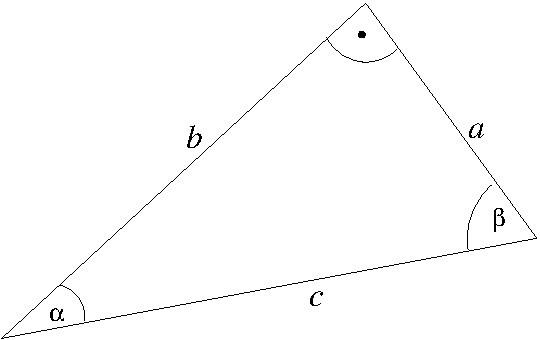
\includegraphics[width=4cm]{img/winkel_aufgaben.pdf}
\end{minipage}




 \item Leite folgende Aussage her: \[ \sin(4\alpha) = 4(\sin\alpha
\cdot \cos^3\alpha - \sin^3\alpha\cdot \cos\alpha)\]
 \item Leite her, dass folgende Aussage gilt:
\[\cos(2\alpha) = 2\cdot\cos^2\alpha -1 \]
 \item* Eine Kugel mit dem Radius 1 umschließt einen Würfel. Bestimme die
maximale Seitenlänge des Würfels.
\end{enumerate}



\section{Exponentialfunktionen und Logarithmus}\label{sec:exponential}

\subsection{Exponentialfunktionen}
Exponentialfunktionen sind Funktionen der Form $f(x) = a^x$, wobei $a$ eine
konstante Zahl~$>0$ ist. Diese Funktionen haben einige gemeinsame
Eigenschaften:
\begin{itemize}
 \item $f(x) > 0$, d.~h. insbesondere die Funktion hat keine Nullstelle
 \item $f(0) = 1$, da $a^0 = 1$ für alle $a$
\end{itemize}

\begin{center}
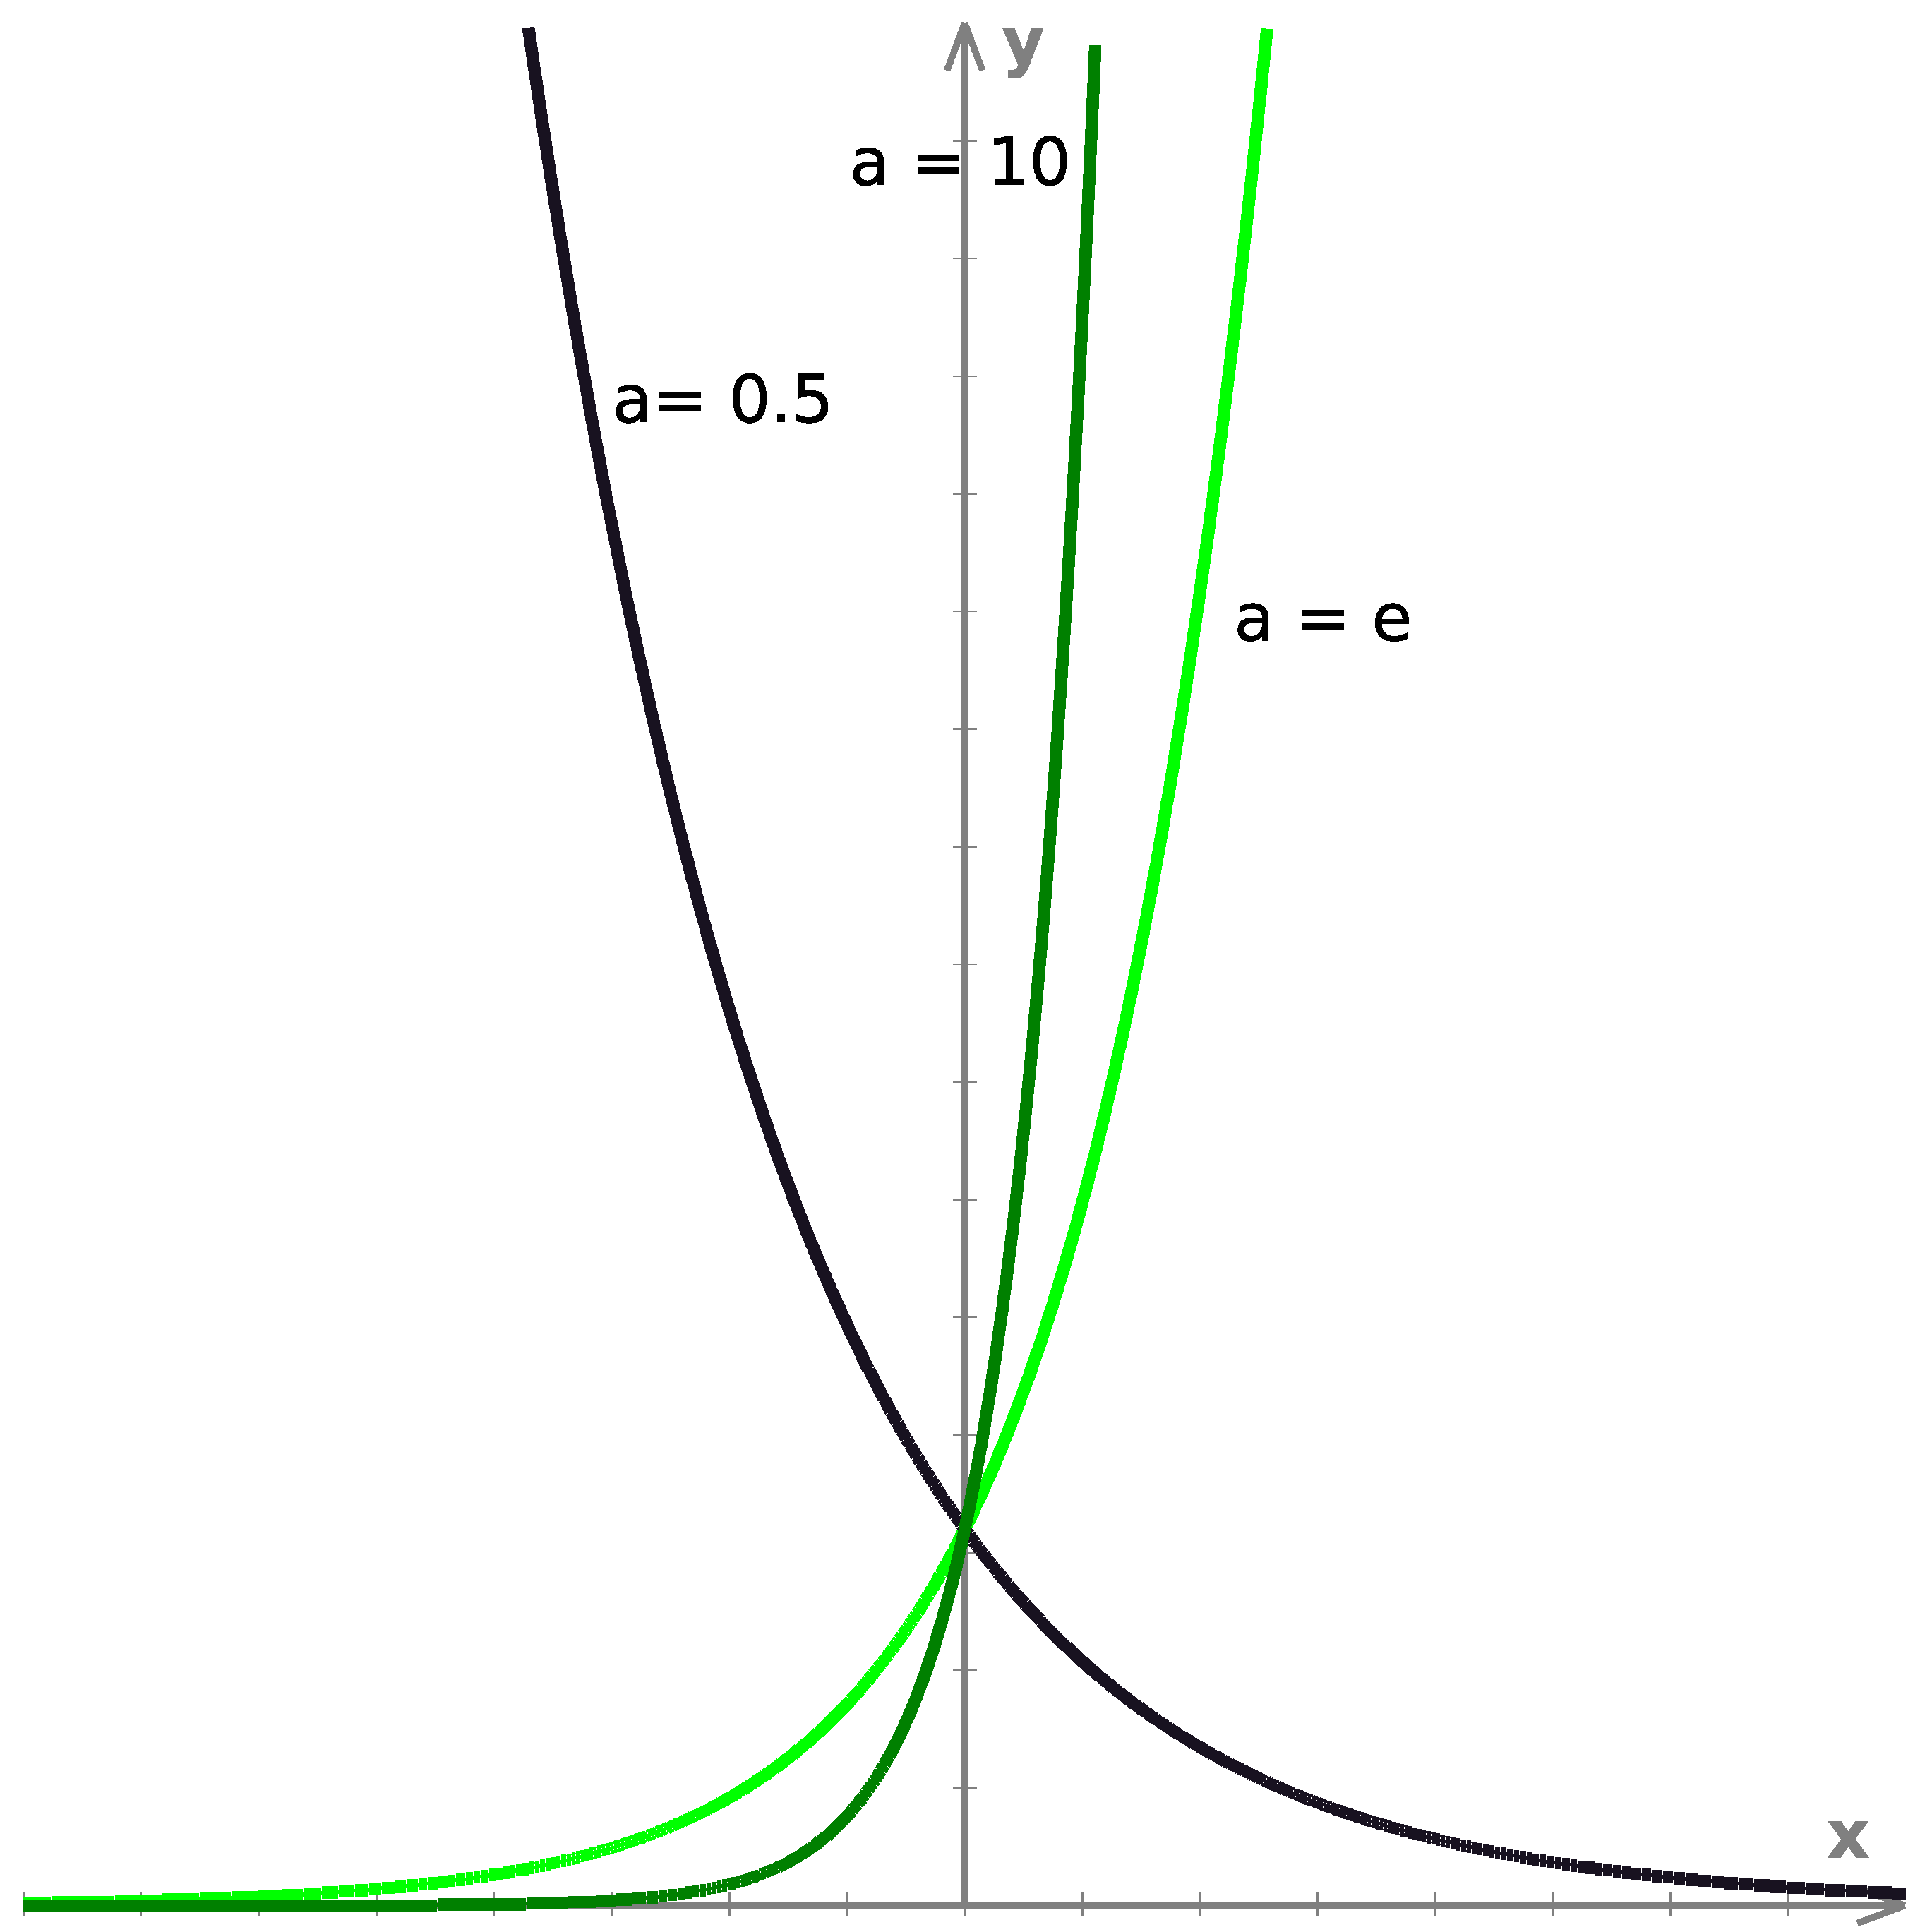
\includegraphics[width=.4\textwidth]{img/exp.pdf} 
\end{center}

\noindent Die Funktion hat abhängig von $a$ folgende Form:
\begin{description}
 \item[$\mathbf{a > 1}$] streng monoton wachsend, für $x \rightarrow -\infty$
geht $f(x)$ gegen $0$.
 \item[$\mathbf{0 < a < 1}$] streng monoton fallend, für $x \rightarrow
\infty$ geht $f(x)$ gegen $0$.
 \item[$\mathbf{a = 1}$] die Funktion ergibt konstant $1$ ($f(x) = 1^x$).
\end{description}

\noindent Eine spezielle Exponentialfunktion ist die $e$-Funktion $f(x) = e^x$, mit 
der sich viele natürliche Vorgänge beschreiben lassen. $e =
2,718281828459\dots$ ist die \emph{Eulersche Zahl}. Die $e$-Funktion hat die
Eigenschaft, dass $e^x = (e^x)' = (e^x)'' = (e^x)^{(n)}$, d.~h. alle Ableitungen der
Funktion sind gleich der Funktion.

\noindent Die Umkehrfunktion der Exponentialfunktionen ist der Logarithmus:
\[y = a^x \Longleftrightarrow x = \log_a y.\]


\subsection{Logarithmus}
Der Logarithmus $\log_a b$ (sprich: Logarithmus von $b$ zur Basis $a$) ist die
Zahl $c$, für die $a^c = b$ gilt. Der Logarithmus ist damit die
Umkehrfunktion der Exponentialfunktion.

\noindent Wichtige Logarithmen sind:

\begin{description}
 \item[Natürlicher Logarithmus] Logarithmus zur Basis $e$: $\log_e x = \ln x$
 \item[Dekadischer Logarithmus] Logarithmus zur Basis $10$: $\log_{10} x = \lg
x$ %(auf Taschenrechner: \emph{log})
 \item[Binärer Logarithmus] Logarithmus zur Basis $2$: $\log_2 x = \text{ld}\,
x$
\end{description}

\subsection{Logarithmusfunktion}
\begin{figure}
\begin{center}
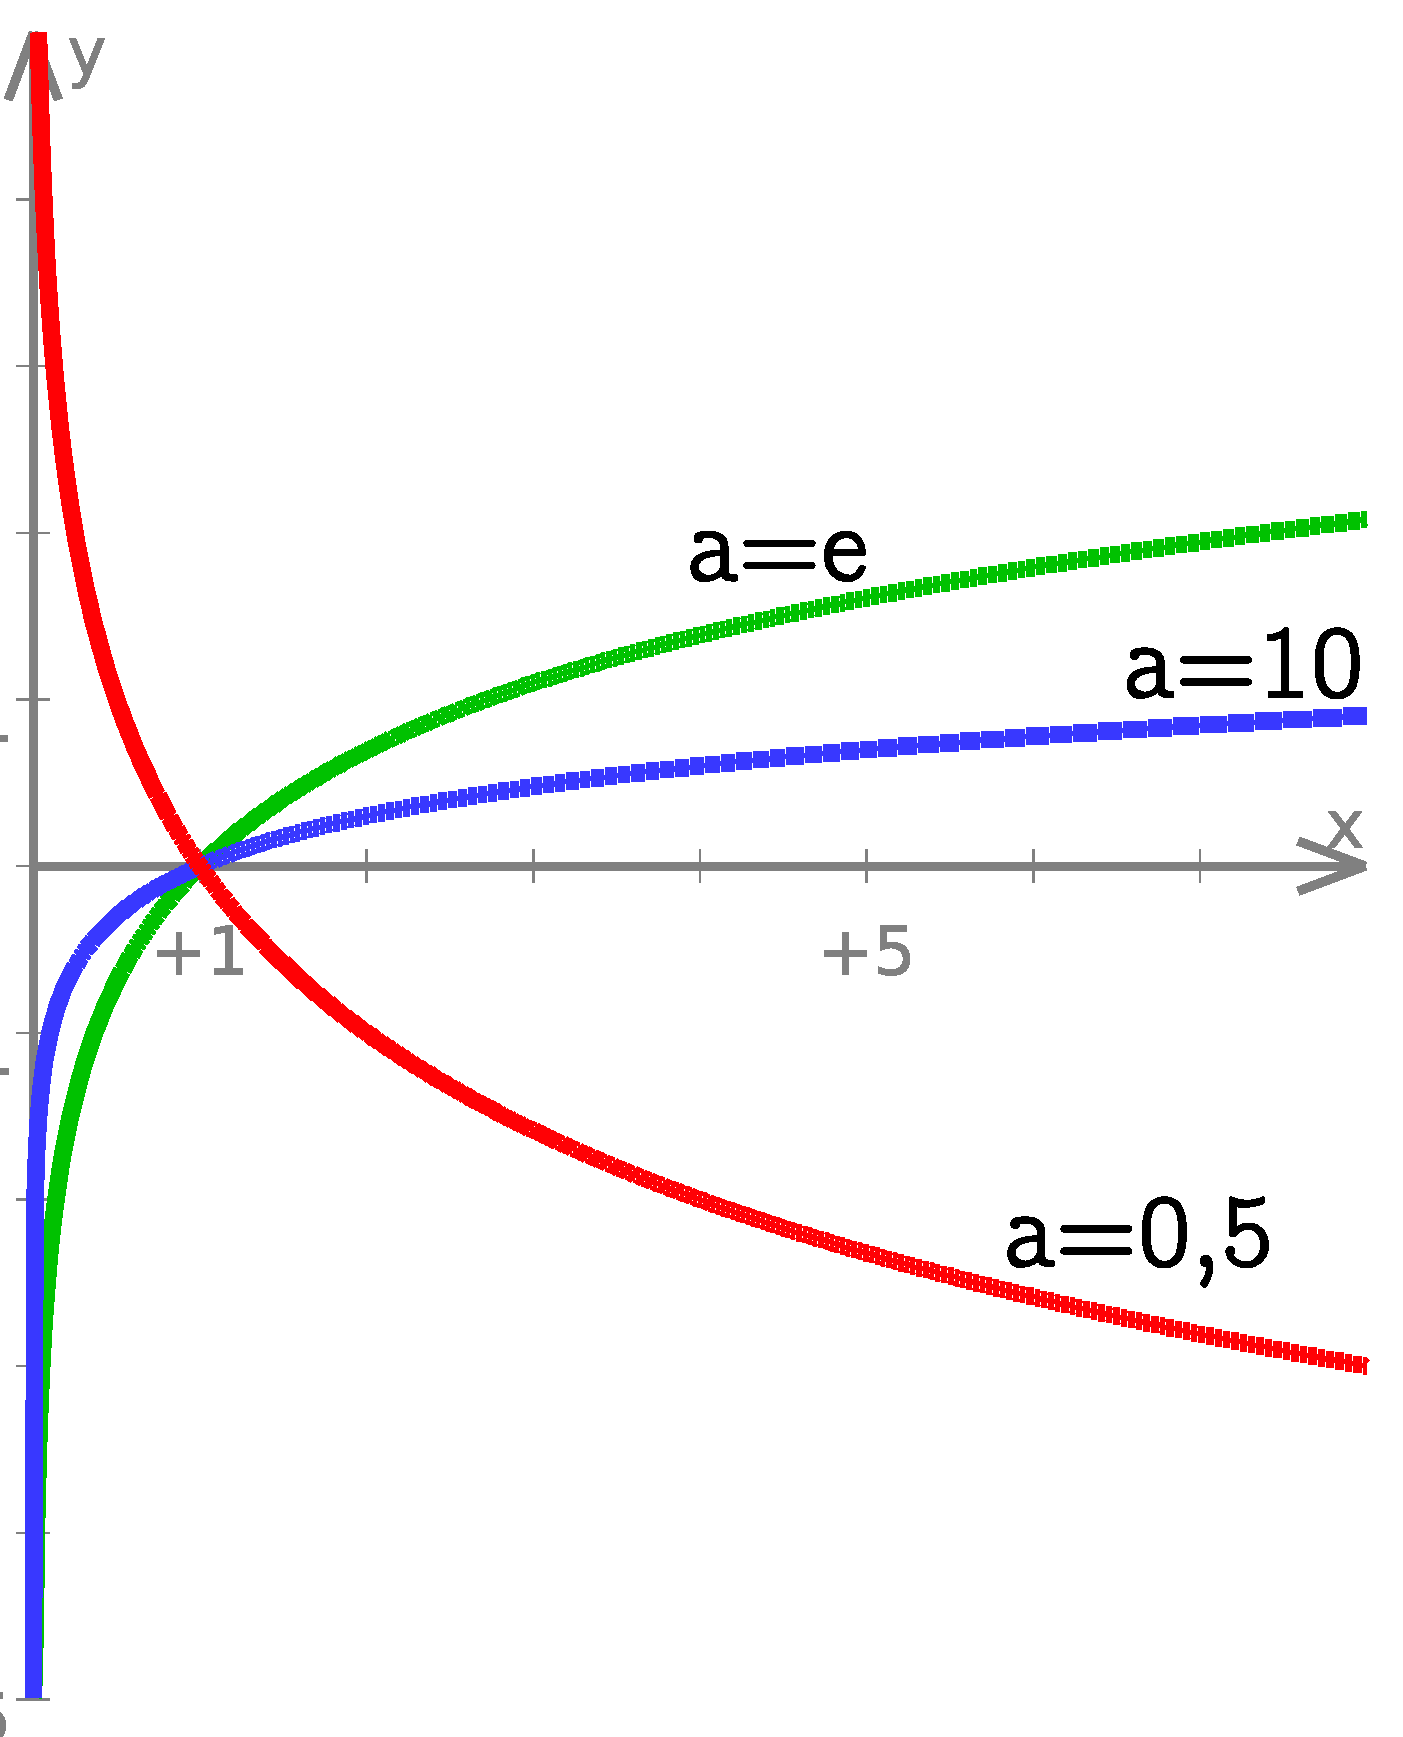
\includegraphics[height=4cm]{img/log.pdf}
\end{center}
\label{fig:logarithmus}
\caption{Graph der Funktion $\log_a x$, mit $a \in\{e, 10, \frac{1}{2}\}$.}
\end{figure}

Der Graph der Logarithmusfunktion (Abbildung 7.3) verhält sich ähnlich wie der Graph der
Exponentialfunktion: Abhängig von $a$ ist der Graph entweder monoton fallend
($0 < a < 1$) oder steigend ($a>1$). Die Funktion ist nur für positive Zahlen
definiert, der Grenzwert für $x \rightarrow 0$ ist $\pm\infty$. Der
Funktionswert $\log_a(1)$ ist $0$, unabhängig von $a$.
Für große Werte von $x$ (und $n > 0$) gilt: $log_a (x) < n\cdot x$, die Logarithmusfunktion wächst also langsamer als eine lineare Funktion.

\subsection{Logarithmengesetze}
\begin{eqnarray*}
\log_a(u\cdot v)  & = & \log_a u + \log_a v \\
\log_a\frac{u}{v} & = & \log_a u - \log_a v \\
\log_a u^r        & = & r\cdot \log_a u 
\end{eqnarray*}

\subsection{Basiswechsel}
Ein Logarithmus zu einer ungewöhnlichen Basis $a$ kann berechnen werden, indem
dieser auf eine andere Basis $b$ gebracht wird:
\[\log_a x = \frac{\log_b x}{\log_b a} \text{, z.~B. } \log_a x =
\frac{\ln x}{\ln a}\]

\noindent Dies ist nützlich, da die meisten Taschenrechner nur die Logarithmen
zur Basis $e$ (Taste \texttt{ln}) und $10$ (Taste \texttt{log}) berechnen
können. Alle anderen Logarithmen müssen auf diese Basen umgerechnet werden.


\subsection{Aufgaben}
\begin{enumerate}
 \item Löse nach $x$:
\begin{multicols}{3}
\begin{enumerate}
 \item $1 = e^x$
 \item $8 = 2^x$
 \item $3= 5e^x$
 \item $e = \frac{e^x}{e}$
 \item $9 = e^{cx}$
 \item $3 = \log_2 x$
 \item $0 = \log_{42} x$
 \item $0 = 5\log_5 x$
 \item $9 = 3\ln e^x$
\end{enumerate}
\end{multicols}

  \item Vereinfache:
  \begin{multicols}{2}
   \begin{enumerate}
    \item $\lg 2 +\lg 5$
    \item $\lg 5 +\lg 6 -\lg 3$
    \item $3\ln a +5\ln b -\ln c$
    \item $2\ln v - \ln v$
    \item $\frac{1}{2}\log_7 9 - \frac{1}{4}\log_7 81$
    \item $\log_3(x-4) + \log_3(x+4) = 3$
    \item $2 \log_2(4-x) + 4 = \log_2(x+5) - 1$ %32x^2 - 257x + 507 = 0
    \item $\log_5 x = \log_5 6 - 2  \log_5 3$ % x = 2/3
   \end{enumerate}
  \end{multicols}

  \item Das Wachstum von Bakterienkulturen lässt sich mit Hilfe der
$e$-Funktion beschreiben. Die Anzahl der Bakterien zum Zeitpunkt $t$ ist eine
Funktion $N(t)$, die abhängig ist von der anfänglichen Anzahl der Bakterien
(also der Wert $N_0 := N(0)$) und der Wachstumsrate $k$ des Bakteriums
(konstant). Es entsteht damit die Formel:
$N(t) = N_0e^{kt}$.

Für $N_0 = 100, k= 0,2$:
\begin{enumerate}
 \item Wieviele Bakterien gibt es zum Zeitpunkt 5 (10, 20, 50, 100)?
 \item Zu welchem Zeitpunkt gibt es 500 (1000, 5000, 10000) Bakterien?
\end{enumerate}

  \item Die Anzahl von Teilchen eines radioaktiven Materials ist ein
Exponentialfunktion der Zeit $N(t) = N_0e^{-\lambda t}$, wobei $N_0$ die
Anzahl der Teilchen zum Zeitpunkt 0 und $\lambda$ die Zerfallskonstante des
Materials ist. Gegeben sind $N_0= 1000, \lambda = 2$.
\begin{enumerate}
  \item Wieviele Teilchen sind zum Zeitpunkt 1 (5, 10, 100) noch vorhanden?
  \item Wie lange dauert es, bis $\frac{1}{4}$ (die Hälfte (Halbwertszeit),
$\frac{3}{4}$, $\frac{7}{8}$) des Materials zerfallen ist?
\end{enumerate}

\end{enumerate}



%\subsection{Literatur}
%Frank, Schulz, Tietz, Warmuth: \textit{Wissenspeicher Mathematik}. 1. Auflg.
%1998. Volk und Wissen Verlag Berlin. 
%Weitere Formeln gibt es in der (umfangreichen) \emph{Formelsammlung
%Trigonometrie} der %Wikipedia\footnote{\url{http://de.wikipedia.org/wiki/Formelsammlung_Trigonometrie}}.

%%weiter siehe Kurvendiskussion
%\addtocontents{toc}{\setcounter{tocdepth}{0}}

%=============================================================================

\section{Kurvendiskussion}
\label{sec:kurvendiskussion}

Autor: Andreas Zöllner

\noindent "Uberarbeitung: Gerhard Gossen

\mbox{}\par

\noindent Eine Kurvendiskussion hilft uns eine Funktion zu "`verstehen"'. Wir bekommen Informationen über die Form des Graphs (z.~B. Anzahl und Lage von Extrema und Wendepunkten) und über wichtige Punkte (z.B. Nullstellen) der Funktion.

\noindent Eine Kurvendiskussion hat eine feste Reihenfolge von Schritten. Einige davon können von Mathematik-Programmen durchgeführt werden, aber bei komplexeren Funktionen ist der eigene Hirnschmalz gefragt.

\subsection{Definitionsbereich}

Als erstes sollte man sich über den Definitionsbereich $D(f)$ der Funktion $f$
im Klaren sein: Für welche Werte $x\in\real$ ist $f(x)$ überhaupt definiert? Die Funktion $\frac{1}{x-1}$ ist beispielsweise für $x=1$ nicht definiert (Division durch 0!), die Logarithmusfunktion ist nur für positive Werte definiert. 

\noindent Isolierte Punkte, an denen $f$ nicht definiert ist, heißen
\textbf{Definitionslücken}. Hierbei unterscheidet man verschiedene Arten von
Definitionslücken, worauf wir hier jedoch nicht näher eingehen wollen.

\noindent Der Definitionsbereich wird als Menge angegeben. Beispiele für verschiedene Bereich gibt Tabelle~\ref{tab:definitionsbereiche}.

\begin{table}[b]
\begin{tabular}{l|p{13em}}
\textbf{Definitonsbereich} & \textbf{Beschreibung}\\
\hline
$D(f) = \R$ & Der Definitionsbereich ist die gesammte Definitionsmenge.\\

$D(f) = \R \setminus \{c\}$ & Die Funktion hat eine Definitionslücke an der Stelle $c$.\\
$D(f) = \{x\in\R\ |\ a < x < b \wedge x\geq c\}$ & $f$ ist nur in den Intervallen $(a,b)$ und $[c,\infty)$ definiert.
\end{tabular}
\vspace{-1em}
\caption{Beispiele für Definitionsbereiche}
\label{tab:definitionsbereiche}
\end{table}



%=============================================================================

\subsection{Wertebereich}

Der Wertebereich einer Funktion lässt sich meist über Betrachtungen zur
Stetigkeit, der Extrema, der Monotonie und der Asymptoten ermitteln.


%=============================================================================

\subsection{Nullstellen}

Eine Stelle $x_0\in{}D(f)$ heißt eine \textbf{Nullstelle} der Funktion $f$,
wenn
\[
f(x_0)
\ =\ 0
\,,
\]
zur Bestimmung der Nullstellen müssen wir daher alle Lösungen der Gleichung \[f(x)\ =\ 0 \] finden.

%=============================================================================

\subsection{Extrema}

Um die Extrema einer Funktion $f$ bestimmen zu können, müssen die ersten beiden Ableitungen von $f$ existieren. Eine Stelle $x_0$ ist ein Extremum von $f$, wenn gilt:
\begin{enumerate}
\item $f'(x_0) = 0$ (\emph{notwendige Bedingung}) 
\item $f''(x_0) \neq 0$ (\emph{hinreichende Bedingung})
\end{enumerate}

\noindent Bei $f''(x)>0$ liegt ein lokales Minimum, bei $f''(x)<0$ ein lokales Maximum vor.
\newline \newline
\noindent Die \textbf{globalen Extrema} erhält man, indem man zusätzlich das Verhalten der
Funktion an den Grenzen des Definitionsbereichs in Betracht zieht. Also z.\,B.
falls $D(f)=\real$ sind dies die Werte $\lim_{x\to\pm\infty}f(x)$.
\newline \newline
\noindent Die erste Ableitung gibt also die Steigung der Tangenten an den Graphen an. Links von einem Maximum ist die Steigung positiv, rechts davon ist sie negativ (siehe Abb.~\ref{fig:tangenten}). Der Nulldurchgang der Ableitung entspricht also einer Tangenten mit der Steigung $0$, also einer horizontalen Gerade. Bei einem Minimum wechselt die Steigung der Tangenten entsprechend von negativ zu positiv.

\begin{figure}
\begin{center}
    \begin{minipage}[b]{.4\textwidth}
    \begin{center}
        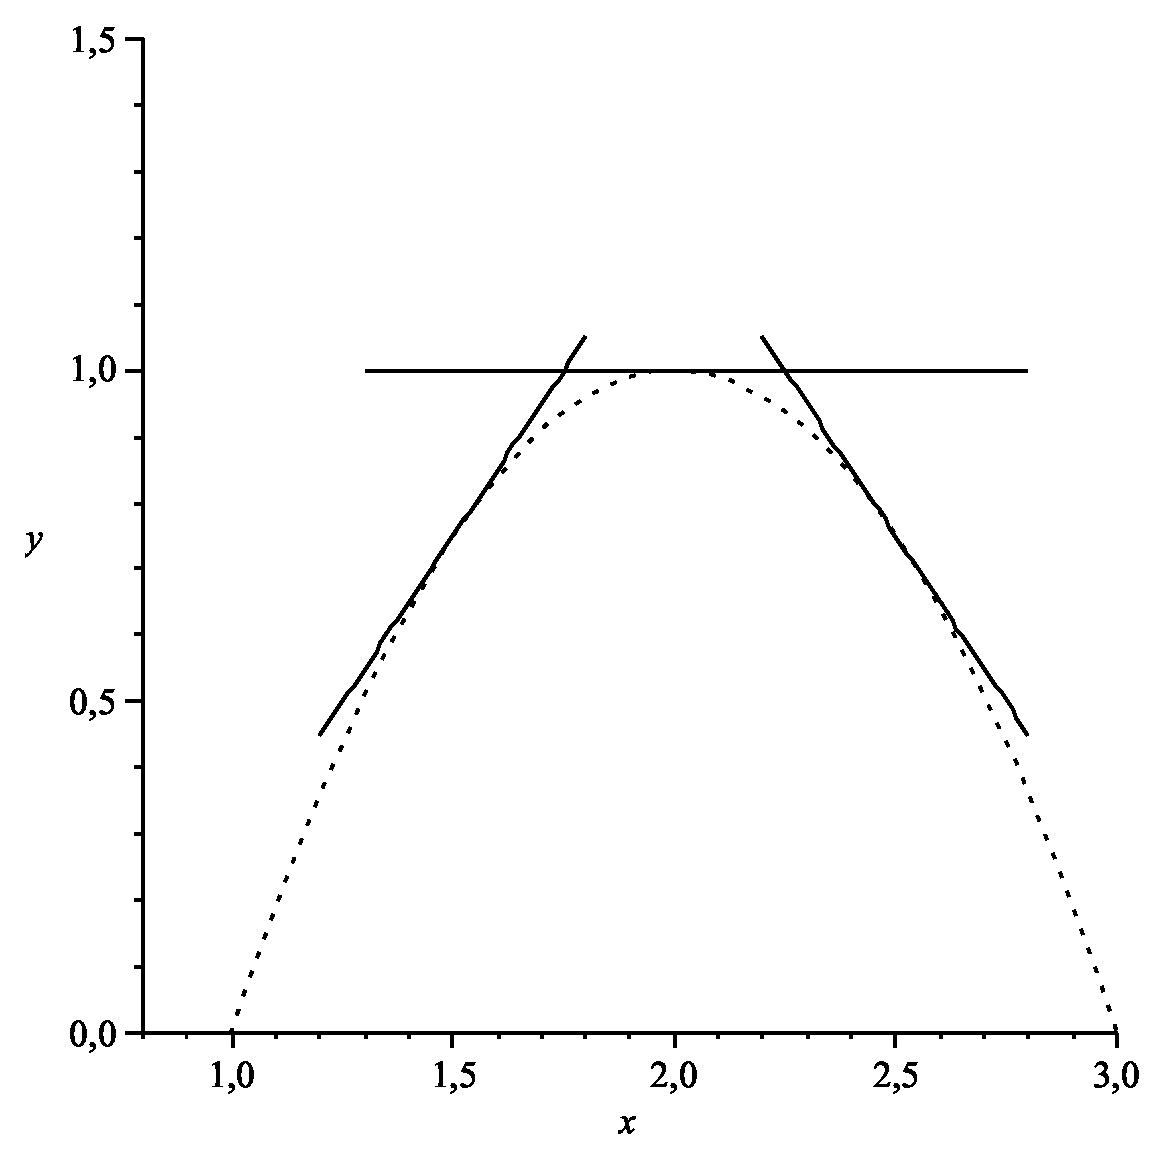
\includegraphics[width=.8\textwidth]{img/tangenten}
    \end{center}
    \caption{Tangenten der Funktion $-(x-2)^2+1$ an den Stellen $\frac{3}{2},2, \frac{5}{2}$}
    \label{fig:tangenten}
    \end{minipage}
    \hspace{.1\textwidth}
    \begin{minipage}[b]{.41\textwidth}
    \begin{center}
        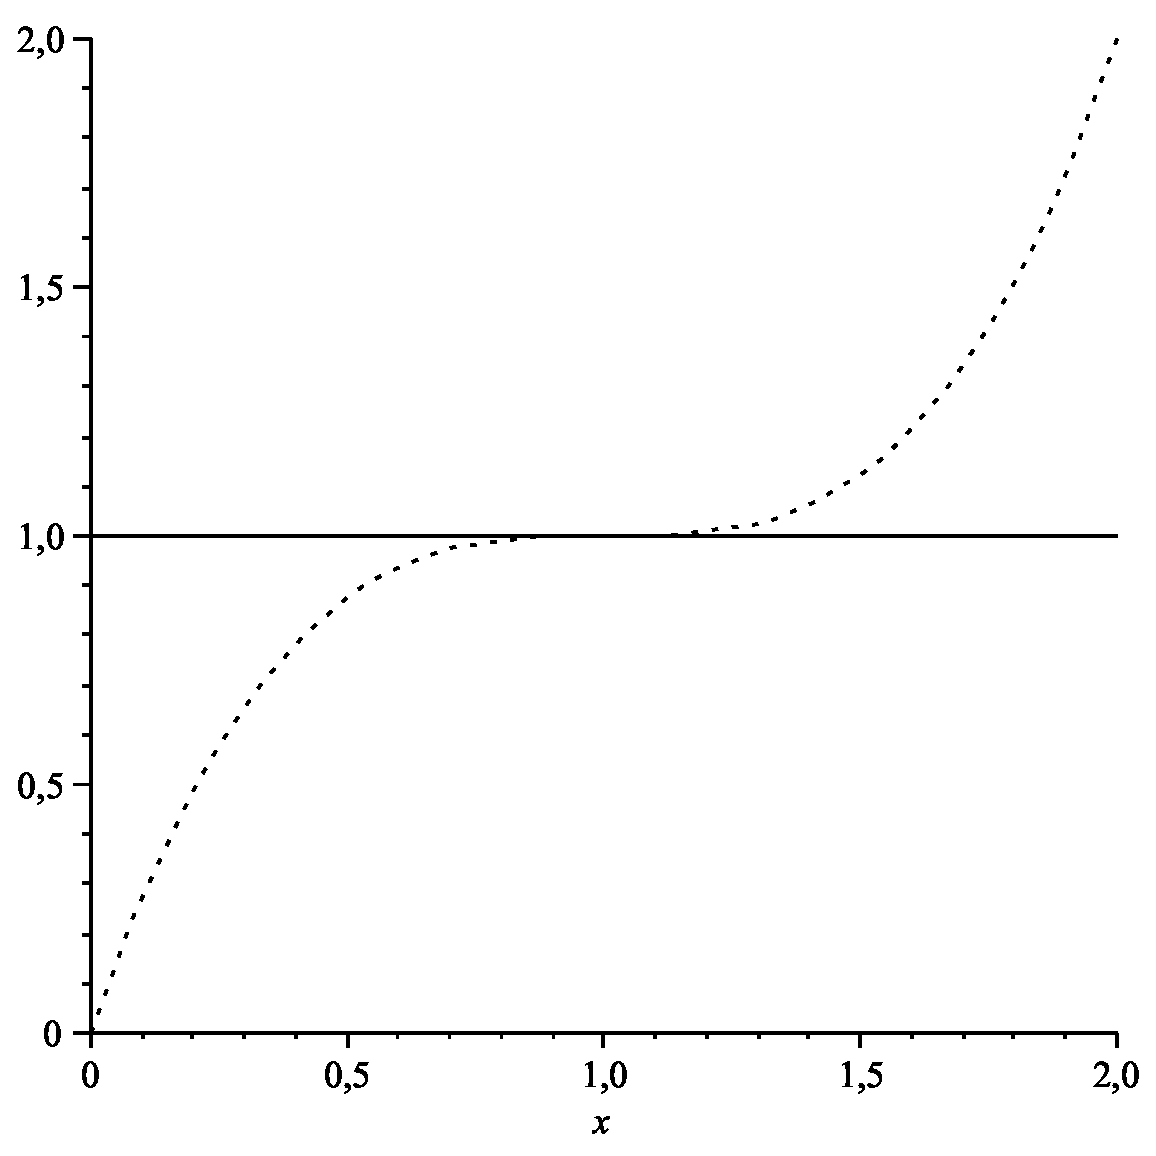
\includegraphics[width=.8\textwidth]{img/sattelpunkt}
    \end{center}

    \caption{Sattelpunkt der Funktion $(x-1)^3+1$ an der Stelle $x=1$}
    \label{fig:sattelpunkt}
    \end{minipage}
\end{center}

\end{figure}
%%%%%%%%%%%%%%%%%%%%%%%%%%%%%%%%%%%%%%%%%%%%%%%%%%%%%%%%%5
\newpage
\subsection{Exkursion: Ableiten einer Funktion} 
%\label{sec:ableitungen}
\subsubsection{Differentiationsregeln}
\begin{enumerate}
\item Faktorregel: $c\cdot f(x)(c \in \mathbb{R},konstant) \Rightarrow c\cdot f'(x)$
\item Summenregel: $f(x) + g(x) \Rightarrow f'(x)+g'(x)$
\item Produktregel:$f(x)\cdot g(x) \Rightarrow f'(x)\cdot g(x) + f(x)\cdot g'(x)$
\item Quotientenregel: $\displaystyle \frac{f(x)}{g(x)} (g(x)\neq 0) \Rightarrow \displaystyle \frac{f'(x)g(x) - f(x)g'(x)}{(g(x))^2}$
\item Kettenregel: $f(g(x)) \Rightarrow f'(g(x))\cdot g'(x)$
\end{enumerate}

\subsubsection{wichtige Ableitungen}
\begin{center}
\begin{tabular}{c|c}
Funktion & Ableitung\\
\hline
$c$ & $0$\\
$x^n$ & $n\cdot x^{n-1}$\\
$sin x$ & $\cos x$\\
$cos x$ &$-\sin x$\\
$tan x $& $\displaystyle \frac{1}{\cos^2 x}$\\
$e^x$ & $e^x$\\
$ln x$ & $\frac{1}{x}$\\
\end{tabular}
\end{center}
%%%%%%%%%%%%%%%%%%%%%%%%%%%%%%%%%%%%%%%%%%%%%%%%%%%%%%
\subsection{Wendepunkte}

An einem \emph{Wendepunkt} ändert sich das Krümmungsverhalten des Funktionsgraphen, der Graph wechselt also von einer Links- in eine Rechtskurve oder umgekehrt.

\noindent Das notwendige Kriterium für eine Wendestelle bei $x_0$ ist, dass der Wert der zweiten Ableitung Null wird: $f''(x_0) = 0$. Zusätzlich muss noch eine der beiden folgenden Bedingungen erfüllt sein:
\begin{description}
    \item[Der Wert der dritten Ableitung ist ungleich Null:] $f'''(x_0)\neq 0$. Dabei muss aber die dritte Ableitung existieren.
    \item[Das Vorzeichen der zweiten Ableitung wechselt in $x_0$:] Falls keine dritte Ableitung existiert oder ihre Berechnung zu aufwändig ist, muss man das Vorzeichen auf beiden Seiten von $x_0$ vergleichen.
\end{description}

\noindent Die zweite Ableitung gibt die Änderung der Steigung an. Wenn die zweite Ableitung positiv ist, wird die Steigung größer, der Graph macht also eine Linkskurve. Eine Rechtskurve entsteht dementsprechend bei einer sinkenden Steigung der Tangente, also einer negativen zweiten Ableitung.

\noindent Eine Spezialform eines Wendepunktes ist der \emph{Sattelpunkt}, bei dem sowohl die erste als auch die zweite Ableitung Null ist. Ein Beispiel dafür zeigt Abbildung~\ref{fig:sattelpunkt}. Hier sieht man, dass es zur Bestimmung der Extrema nicht ausreicht, eine Nullstelle der ersten Ableitung zu finden, es muss auch die zweite Ableitung überprüft werden.

\subsection{Verhalten im Unendlichen, Polstellen, Asymptoten}

Unter dem Verhalten der Funktion $f$ im Unendlichen versteht man die
Grenzwerte
\[
\lim_{x\to\infty}f(x)
\qqtext{bzw.}
\lim_{x\to-\infty}f(x)
\,,
\]
sofern diese existieren.

\noindent Die Asymptoten beschreiben das Verhalten der Funktion $f$ im Unendlichen und
an Polstellen (eine Art von Definitionslücken) genauer. Der Begriff "`asymptotisch"' bedeutet dabei "`sich
an"-nähernd"'. Eine \textbf{Asymptote} der Funktion $f$ ist eine lineare
Funktion
\[
y
\ =\ mx+n
\quad\text{für gewisse $m,n\in\real$}
\,,
\]
der sich die Funktion $f$ annähert.

\subsection{Graph der Funktion}

Mit Hilfe dieser Informationen kann man den Graphen der Funktion jetzt gut zeichnen. Dazu zeichnet man Nullstellen, Extrema, Wendepunkte und eventuelle Asymptoten auf und hat damit schon die Grobstruktur gegeben. Falls nötig, kann man noch die Funktionswerte für einzelne Stellen berechnen, um etwa die Stärke der Krümmung zu erkennen.

%\subsection{Anwendungen}

%=========================================================================
%================================================================================
\subsection{Übungsaufgaben}

%--------------------------------------------------------------------------------
\begin{enumerate}
\item
Führen Sie eine vollständige Kurvendiskussion für die Funktionen durch:
\[
f(x)
= -x^3 + 3 x - 2
\]
\[f(x) = x^3 - 4x^2 + 5x -2\]

%--------------------------------------------------------------------------------
\item
Führen Sie eine Kurvendiskussion für die Funktion
\[
g(x)
\ =\ \frac{3 x^4 - 12 x^3 + 9 x^2 + 12 x - 12}{x^3 - 4 x^2 + 5 x - 2}
\]
durch.

%--------------------------------------------------------------------------------
\item
Führen Sie eine Kurvendiskussion für die Funktion
\[
f(x)
\ =\ 2\sin(x\cdot\pi)
\]
durch.

Es soll nun ein Dreieck $ABC$ unter den Graphen der Funktion gelegt werden.
Dieses sei durch die Punkte $A(0,0)$, $B(x,0)$ und $C(x,f(x))$ für
$x\in\cinterval01$ gegeben. Berechnen Sie die Stelle $x$ so, dass die Maßzahl
des Flächeninhalts des Dreiecks $ABC$ maximal wird.
\end{enumerate}


%=============================================================================

%\subsection{Literatur}

%\renewcommand{\labelenumi}{[\arabic{enumi}]}
%\renewcommand{\theenumi}{[\arabic{enumi}]}
%\begin{enumerate}
%\item
%I. N. Bronstein et al. \textit{Teubner-Taschenbuch der Mathematik}. (2 Bände)
%B.\,G. Teubner Leipzig, 1996.

%\item
%K. Vetters. \textit{Formeln und Fakten im Grundkurs Mathematik}. B.\,G. Teubner Stuttgart, 2004.

%\end{enumerate}

%\end{document}

\def\vect#1,#2{\left(\!\!\!\begin{array}{c}#1\\#2\end{array}\!\!\!\right)}
\newcommand{\mvect}[1]{\left(\!\!\!\begin{array}{c}#1%
\end{array}\!\!\!\right)}

\chapter{Vektoren}
	
	Autor: Gerhard Gossen
	
\noindent	\"Uberarbeitung: Marko Rak, Melanie Pflaume
	
	\section{Definition}
	
		Der Vektor \[\overrightarrow{
        x
        }
         = \mvect{ x_1\\ x_2 \\ \vdots \\ x_n}\] ist
		ein $n$-dimensionaler Vektor. Die \emph{Komponenten} $x_1, x_2,
		\dots, x_n$ sind reelle Zahlen. In der Vorlesung wird statt
		$\overrightarrow{x}$ meist nur $x$ geschrieben.
		
		\noindent Geometrisch interessant sind Vektoren der Dimension 2 \[x =
		\mvect{x\\y} \text{ und Dimension 3: } x = \mvect{x\\y\\z}.\] Sie können als
		Pfeile in
		eine bestimmte Richtung dargestellt werden. Man kann sie auch als
		\emph{Verschiebung} interpretieren.
		Der Nullvektor $\overrightarrow0$ bzw. $0$ ist der Vektor, bei dem alle
		Komponenten $0$ sind.
		Der \emph{Ortsvektor} eines Punktes $P$ ist der Vektor 
		zwischen dem Ursprung des Koordinatensystems und $P$.
		Ein \emph{Skalar} ist eine einzelne Zahl vom selben Typ wie $x_1, x_2, \dots,
		x_n$.
		
		\begin{center}
			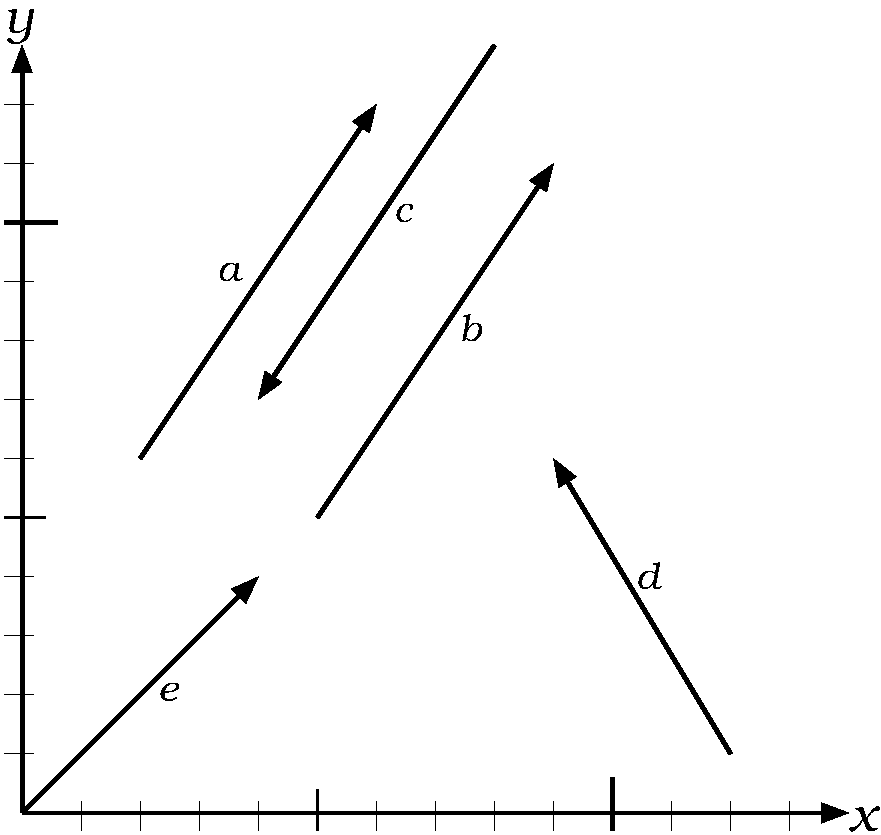
\includegraphics[width=.3\textwidth]{img/vektoren.pdf}
			
			{\scriptsize$a = \vect4,6 = b,\ c = \vect-4,{-6}=-1\cdot a,\ d= \vect{-3},5,\
			e=\vect4,4$}
		\end{center}
	
	\section{Operationen}
	
		\subsection{Addition und Subtraktion}
			Zwei Vektoren werden addiert, indem die einzelnen Komponenten addiert werden:	
			\[x + y = \mvect{x_1 \\ x_2 \\ \vdots \\ x_n} +
			\mvect{y_1 \\ y_2 \\ \vdots \\ y_n} = \mvect{x_1 + y_1 \\ x_2 + y_2 \\ \vdots
			\\ x_n + y_n}\]
		
			Die Subtraktion ist analog:
			\[x - y = \mvect{x_1 \\ x_2 \\ \vdots \\ x_n} - \mvect{y_1 \\ y_2 \\ \vdots \\
			y_n} = \mvect{x_1 - y_1 \\ x_2 - y_2 \\ \vdots \\ x_n - y_n}\]
			
			Beispiele:
			\[\hspace{-6.23pt}
            \begin{array}{ccc}
				\mvect{2\\4}+\mvect{6\\7} = \mvect{8\\11}  &\mvect{3\\7}+\mvect{0\\0}
				= \mvect{3\\7} & \mvect{1\\2\\3}+\mvect{4\\5\\6}=\mvect{5\\7\\9}\\
				\mvect{2\\4}-\mvect{6\\7} = \mvect{-4\\-3} &\mvect{3\\7}-\mvect{0\\0}
				= \mvect{3\\7} & \mvect{12\\-5\\0}-\mvect{-7\\4\\3}=\mvect{19\\-9\\-3}
			\end{array}\]
			
			\noindent Geometrisch gesehen entspricht die Addition der Vektoren $a$ und $b$
			der Verschiebung, die durch Verschieben zuerst in Richtung $a$ und danach in
			Richtung $b$ entsteht. Wie man in der Zeichnung erkennt, ist die Addition
			\emph{kommutativ}, d.\,h. $a+b = b+a$.
			\begin{center}
				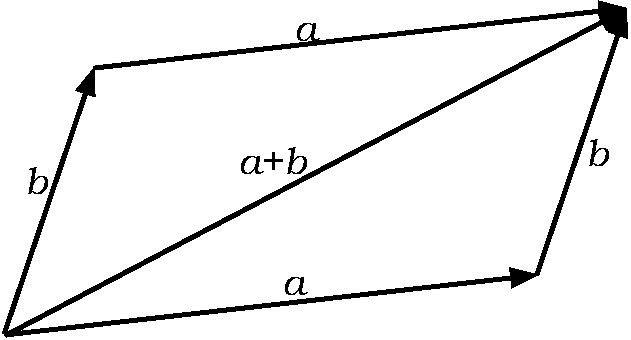
\includegraphics[height=2cm]{img/vektor_addition} 
			\end{center}
	
		\subsection{Multiplikation mit einem Skalar}
			Ein Vektor wird mit einem Skalar multipliziert, indem jede einzelne
			Komponente mit dem Skalar multipliziert wird:
			\[\lambda\cdot x = \lambda\cdot \mvect{x_1 \\ x_2 \\ \vdots \\ x_n} =
			\mvect{\lambda\cdot x_1 \\ \lambda\cdot x_2 \\ \vdots \\ \lambda\cdot x_n}\]
			Die Multiplikation mit dem Skalar $0$ ergibt immer den Nullvektor.
			
			Beispiele:
			\[\hspace{-15.14pt}\begin{array}{cccc}
				 1\cdot\mvect{3\\6\\4}=\mvect{3\\6\\4} & 2\cdot\mvect{1\\2\\3}=\mvect{2\\4\\6} &
				 -1\cdot\mvect{3\\-3\\3} = \mvect{-3\\3\\-3} &
                 0\cdot
				\mvect{3\\5\\1}=\mvect{0\\0\\0}
			\end{array}\]
			
			Geometrisch entspricht die Multiplikation einer \emph{Streckung} um den
			Faktor $\lambda$.
			
			\begin{center}
				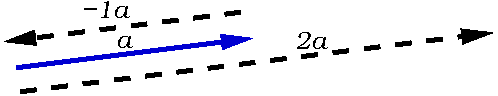
\includegraphics[width=.4\textwidth]{img/vektor_mult.pdf}
				
				{\scriptsize Vektor $a$, skaliert mit $\lambda = -1$ (oben) und $\lambda = 2$
				(unten).}
			\end{center}
	
	\section{Linearkombination}
		
		Jeder Vektor $b$, der sich als Summe $b = \lambda_1 a_1 + \lambda_2 a_2 +
		\dots + \lambda_n a_n$ darstellen lässt, heißt \emph{Linearkombination} der
		Vektoren $a_1, a_2, \dots, a_n$. Die $\lambda_i$ sind reelle Zahlen.
		
	\section{Lineare Abhängigkeit}
	
		Die Vektoren $a_1, \dots a_n$ sind \emph{linear unabhängig}, wenn die
		Gleichung 
		\[\lambda_1 a_1 + \lambda_2 a_2 + \dots + \lambda_n a_n = \overrightarrow 0\]
		nur die triviale Lösung $\lambda_1 = \lambda_2 = \dots = \lambda_n = 0$ hat. Ansonsten
		sind die Vektoren \emph{linear abhängig}.
		
		\noindent Wenn zwei oder mehr Vektoren linear abhängig sind, so kann ein Vektor als
		Linearkombination der anderen Vektoren dargestellt werden.
		
		\noindent Beispiel:
		Die Vektoren \[\mvect{2\\5\\1},\mvect{6\\2\\8},\mvect{5\\6\\5}\] sind linear
		abhängig, da \[1 \cdot \mvect{2\\5\\1} + \frac{1}{2} \cdot \mvect{6\\2\\8} =
		\mvect{5\\6\\5} \text{ bzw. } 1 \cdot \mvect{2\\5\\1} + \frac{1}{2} \cdot
		\mvect{6\\2\\8} + (-1) \cdot \mvect{5\\6\\5} = 0.\]
		
	\section{Betrag eines Vektors}
		
		Der Betrag $|a|$ eines Vektors entspricht der Länge dieses Vektors. Er wird
		berechnet als \[|a| = \left| \mvect{a_1\\ \vdots \\ a_n} \right| =
		\sqrt{\sum_{i=1}^n a_i^2}\] 
		
		Beispiele:
		\begin{align*}
			\left| \mvect{1\\0}\right| &= \sqrt{1^2+0^2} = \sqrt{1} = 1\\
			\left| \mvect{3\\4}\right| &= \sqrt{3^2+4^2} = \sqrt{25} = 5\\
			\left|\mvect{2\\-3\\1\\7\\-1}\right| &= \sqrt{2^2+(-3)^2+1^2+7^2+1^2} =
			\sqrt{4+9+1+49+1} = \sqrt{64} = 8
		\end{align*}
        
        Manchmal wird der Betrag auch anders definiert.
		
	\section{Skalarprodukt}
		Das Skalarprodukt $(a,b)$  der beiden Vektoren $a$ und $b$
		ist die reelle Zahl \[(a,b) =|a||b|\cos\alpha,\] wobei $\alpha$ der Winkel
		zwischen den
		Vektoren ist (andere Schreibweise: $a\cdot b$).
		
		\noindent Durch Umstellen entsteht eine Formel zur Bestimmung des Winkels $\alpha$:
		\begin{align*}
\cos\alpha &= \frac{(a,b)}{|a| |b|} = \frac{a_1b_1+a_2b_2+\dots
		a_nb_n}{\sqrt{a_1^2+a_2^2+\dots a_n^2}\sqrt{b_1^2+b_2^2+\dots b_n^2}} \\&
		\left( = \frac{\sum_{i=1}^n a_ib_i}{\sqrt{\sum_{i=1}^n a_i^2}\ 
		\sqrt{\sum_{i=1}^n b_i^2} } \right)\end{align*}
		
		\noindent Meist will man überprüfen, ob zwei Vektoren orthogonal zueinander sind. Mit \\
		$\cos(90^\circ) = \cos(\frac{\pi}{2}) = 0$ ergibt sich:
		\begin{equation*}
			\frac{(a,b)}{|a||b|} = 0
		\end{equation*}
	\newpage
		Beispiele:
		\begin{enumerate}
			\item Winkel zwischen $\vect1,0$ und $\vect0,1$:
			\begin{align*}
				\cos\alpha &=
				\frac{\left(\vect1,0,\vect0,1\right)}{\left|\vect1,0\right|\left|\vect0,
				1\right| }
				= \frac{1\cdot0+0\cdot1}{1\cdot1} = 0\\
				\alpha &= \arccos(0) = \frac{\pi}{2} = 90^\circ 
			\end{align*}
			
			\item Winkel zwischen $a= \mvect{-4\\2\\-2}$ und $b=\mvect{10\\-5\\5}$
			\begin{align*}
				\cos\alpha &= \frac{\left(a, b\right)}{|a||b|}\\
				            &= \frac{-40+(-10)+(-10)}{\sqrt{24}\sqrt{150}} 
				            = \frac{-60}{\sqrt{4\cdot6}\sqrt{25\cdot6}} \\
				            &= -\frac{60}{2\sqrt{6}\cdot 5\sqrt{6}} = -\frac{60}{60} = -1\\
				\alpha      &= \arccos(-1) = \pi = 180^\circ
			\end{align*}
	
		\end{enumerate}
		
		\textbf{Hinweis:}
		
		 Das Skalarprodukt zweier Vektoren n'ter Ordnung lässt sich auch folgendermaßen berechnen:\\
		\[ (\left( \begin{array}{l}
				x_{1} \\
				x_{2} \\
				\vdots \\
				x_{n}				
			\end{array} \right) ,
			\left( \begin{array}{l}
				y_{1} \\
				y_{2} \\
				\vdots \\
				y_{n}				
			\end{array} \right) )
			=
			\sum_{i=1}^{n} x_{i} \cdot y_{i}
		\]
	
	\section{Kreuzprodukt}
	
		Das \emph{Kreuzprodukt} zweier Vektoren $a$ und $b$ (beide ungleich dem
		Nullvektor) ist ein neuer Vektor. Dieser ist orthogonal zu $a$ und $b$.
		Schreibweise: $a \times b$.
		
		\noindent Das Kreuzprodukt für 3-dimensionale Vektoren wird so berechnet:
		\[a\times b = \mvect{a_1\\a_2\\a_3}\times \mvect{b_1\\b_2\\b_3} =
		\mvect{a_2b_3 - a_3b_2\\ a_3b_1 - a_1b_3\\ a_1b_2 - a_2b_1}\]
		\newline
		
		\noindent Merkhilfe: Der Wert an der Stelle $\bullet$ ergibt sich aus
		$(1)\cdot(2)-(3)\cdot(4)$, wobei $(1),\dots, (4)$ aus der Formel zu entnehmen
		sind.
		\[\hspace{-7pt}\mvect{\bullet\\\phantom{c_2} \\ \phantom{c_3}} =
		\mvect{\phantom{a_1}\\1\\3}\times
		\mvect{\phantom{b_1}\\4\\2} \quad \mvect{\phantom{c_2} \\ \bullet\\
		\phantom{c_3}} =
		\mvect{3\\\phantom{a_1}\\1}\times
		\mvect{2\\\phantom{b_1}\\4}
		 \quad \mvect{\phantom{c_2} \\ \phantom{c_3}\\ \bullet} =
		\mvect{1\\3\\\phantom{a_1}}\times
		\mvect{4\\2\\\phantom{b_1}}\]
		\newline
		Beispiele:
		\begin{align*}
			\mvect{1\\2\\3}\times \mvect{4\\5\\6} &= \mvect{2\cdot 6-3\cdot 5\\ 3\cdot 4
			- 1\cdot 6\\ 1\cdot 5 - 2\cdot 4} = \mvect{-3\\ 6 \\ -3} \\
			\mvect{1\\0\\0} \times \mvect{0\\ 1 \\ 0} &= \mvect{0\cdot0 - 0\cdot1\\
			0\cdot0 - 1\cdot 0\\ 1\cdot1 - 0\cdot0} = \mvect{0\\0\\1}
		\end{align*}
	
%	\section{Literatur}
		
%		Frank, Schulz, Tietz, Warmuth: \textit{Wissenspeicher Mathematik}. 1. Auflg.
%		1998. Volk und Wissen Verlag Berlin. 
		
	\section{Aufgaben}
		
		\begin{enumerate}
			\item Berechne die Vektoren, mit \[a = \mvect{2\\3\\-1}, b= \mvect{-4\\1\\5},
			c = \mvect{-2\\-2\\-2}, d = \mvect{7\\9\\1}:\]
				\begin{multicols}{2}
					\begin{enumerate}
					   \item $a+b-c+d$
					   \item $d-c-b-a$
					   \item $3a-2b+c$
					   \item $a-\frac{1}{2}c+(-3)b+2d$
					   \item $2a-b+5c-d$
					   \item $3a-5b+4c+2d$
			  		\end{enumerate}
				\end{multicols}
			\item Berechne die Länge der Vektoren:
			\begin{multicols}{3}
				\begin{enumerate}
				    \item $\mvect{0\\1\\0}$
				    \item $\mvect{2\\3\\2}$
				    \item $\mvect{4\\3\\5}$
				    \item $\mvect{-2\\2\\1}$
				    \item $\mvect{3\\-3}$
				    \item $\mvect{2\\-2\\2\\2}$
				\end{enumerate}
			\end{multicols}
			\pagebreak
			\item Bestimme das Skalarprodukt der Vektoren:
			\begin{multicols}{3}
				\begin{enumerate}
				    \item $\mvect{0\\0\\1},\mvect{0\\1\\0}$
				    \item $\mvect{2\\-1\\-3}, \mvect{-2\\1\\3}$
				    \item $\mvect{3\\4\\2},\mvect{2\\-7\\5}$
			    \end{enumerate}
			\end{multicols}
			\item Bestimme den eingeschlossenen Winkel:
			\begin{multicols}{2}
				\begin{enumerate}
			    	\item $\mvect{1\\1\\0},\mvect{0\\\sqrt{2}\\0}$
			    	\item $\mvect{3\\2\\1},\mvect{-5\\1\\13}$
			    \end{enumerate}
			\end{multicols}
       
			\item Berechne das Kreuzprodukt:
				\begin{multicols}{3}
			    	\begin{enumerate}
			        	\item $\mvect{2\\5\\3}\times\mvect{-1\\2\\2}$
			        	\item $\mvect{1\\0\\2}\times\mvect{3\\4\\7}$
			        	\item $\mvect{-2\\-3\\-1}\times\mvect{-4\\-2\\-7} $
			      	\end{enumerate}
			    \end{multicols}
			\item Überprüfe, ob die Vektoren linear abhängig sind. In diesem Fall stelle
			einen der Vektoren als Linearkombination der anderen dar. (Hinweis: Nutze den Gauss-Algorithmus)
			\begin{multicols}{2}
				\begin{enumerate}
					\item $\vect1,0 , \vect1,1$
				    \item $\vect3,5 , \vect5,3$
				    \item $\vect1,2 , \vect7,3 , \vect17,5$
				    \item $\mvect{1\\0\\0}, \mvect{2\\5\\0}, \mvect{3\\7\\1}$
				    \item $\mvect{7\\2\\5}, \mvect{3\\-5\\8}, \mvect{10\\-3\\13}$
				    \item $\mvect{-2\\-3\\4}, \mvect{1\\0\\1}, \mvect{7\\6\\5}$
				    \item $\mvect{3\\7\\5}, \mvect{-2\\5\\1}, \mvect{-7\\3\\-3}$
				    \item $\mvect{1\\0\\1\\1}, \mvect{0\\1\\1\\1}, \mvect{0\\1\\3\\2},
					\mvect{1\\1\\0\\1}$
				    \item $\mvect{1\\0\\2\\1}, \mvect{1\\0\\1\\1},
					\mvect{0\\1\\0\\1}, \mvect{0\\0\\1\\1}$
				\end{enumerate}
			\end{multicols}
		\end{enumerate}

%=============================================================================
\chapter{Komplexe Zahlen}\label{chap:complex}

\paragraph*{Autor:} Andreas Zöllner

%================================================================================
\section{Historie}

Es gibt keine reelle Zahl $x\in\real$, die die Gleichung
\[
x^2
\ =\ -1
\]
erfüllt. Zur Formulierung von Lösungen dieser Gleichung muss eine
Zahlbereichserweiterung durchgeführt werden. Deshalb führte R. Bombielli Mitte
des 16.~Jahrhunderts das Symbol $\sqrt{-1}$ ein, für das L. Euler später
$\imag$ schrieb. Diese \textbf{imaginäre Einheit} ist definiert als eine
Lösung der Gleichung
\[
\imag^2
\ =\ -1
\,.
\]
{%\footnotesize
Man beachte, dass $\imag$ \emph{nicht} definiert ist als $\sqrt{-1}$. Dies hat
den Grund, dass die Gleichung $x^2=-1$ keine \emph{eindeutige} Lösung hat --
ihre andere Lösung ist $-\imag$.
%Dies hat den Grund, dass die Wurzel-Funktion als Funktion auf $\real$ för negative Argumente nicht definiert ist, und als Funktion auf den komplexen Zahlen nicht in die komplexen Zahlen, sondern in deren Potenzmenge abbildet. Das Radizieren hat ja bereits in den reellen Zahlen keine eindeutige L�sung. Z.\,B. besitzt die Gleichung $x^2=1$ die beiden L�sungen $-1$ und $1$, und man definiert $\sqrt{z}$ als die \emph{nichtnegative} L�sung der Gleichung $x^2=z$. Alternativ w�re es auch hier m�glich, die Wurzel-Funktion als Funktion von den reellen Zahlen in deren Potenzmenge zu definieren, so dass z.\,B. $\sqrt{1}\coloneqq\{-1,1\}$.
}

\noindent Euler entdeckte auch die für alle $x,y\in\real$ gültige Formel
\begin{equation}
\label{eq:EulerscheFormel}
\e^{x+\imag y}
\ =\ \e^x\,(\cos y + \imag \sin y)
\,.
\end{equation}

%================================================================================
\section{Kartesische Darstellung}

Eine \textbf{komplexe Zahl} $z$ ist ein Symbol der Form
\begin{equation}
\label{eq:KartesischeForm}
z
\ =\ x\ +\ \imag y
\qquad
\text{mit $x,y\in\real$}.
\end{equation}
Die \textbf{Menge der komplexen Zahlen} wird mit $\complex$ bezeichnet,
\[
\complex
\ =\ \{\;x+\imag y\;|\;x,y\in\real\;\}
\,.
\]

\noindent Aus dieser \textbf{kartesischen Darstellung} $z=x+\imag y$ der komplexen Zahl
$z\in\complex$ ergibt sich die Veranschaulichung von $z$ als geordnetes Paar
bzw.\ zweidimensionaler Vektor $(x,y)\in\real^2$, d.\,h.\ als Punkt der
\textbf{Gaußschen Zahlenebene}.
\newline
\noindent Für eine komplexe Zahl $z=x+\imag y$ mit $x,y\in\real$ bezeichnen
\[
\re(z)
%\ \coloneqq\ \Re(z)
\ \coloneqq\ x
\qqtext{und}
\im(z)
%\ \coloneqq\ \Im(z)
\ \coloneqq\ y
\]
den \textbf{Realteil} bzw.\ \textbf{Imaginärteil} von $z$. Damit ist also
\[
z
\ =\ \re(z)+\imag\cdot\im(z)
\,.
\]

\noindent Die Menge $\real$ der reellen Zahlen ist offensichtlich die Teilmenge der
komplexen Zahlen $z\in\complex$ mit $\im(z)=0$. Die komplexen Zahlen mit
$\re(z)=0$ heißen die \emph{rein imaginären Zahlen}.

%================================================================================
\section{Rechenoperationen}

Mit den komplexen Zahlen wird nach den in $\real$ üblichen Rechenregeln
gerechnet. Dabei wird $\imag$ wie eine Variable behandelt, für die
$\imag^2=-1$ gilt, d.\,h.\ beim Rechnen auftretende Potenzen $\imag^k$ werden
wieder auf $\imag=\imag^1$ zurückgeführt, so dass wieder eine kartesische
Darstellung einer komplexen Zahl als Ergebnis der Rechnung vorliegt.

\noindent Hierbei benötigt man noch das folgende Konzept: Die \textbf{konjugiert komplexe Zahl} zu $z=x+\imag y$ ist die komplexe Zahl
\[
\konj{z}
\ =\ \konj{x+\imag y}
\ \coloneqq\ x-\imag y
\qquad
\text{für $x,y\in\real$}.
\]
Grafisch interpretiert in der Gaußschen Zahlenebene entspricht dies der
Spiegelung an der reellen Achse.

\centerline{\includegraphics[width=7cm]{img/complex1}}

Es ergeben sich nun die grundlegenden Rechenoperationen. Seien $a,b,c,d\in\real$.
\begin{itemize}
\addtolength{\itemsep}{-1em}
\item{}Addition. Sie erfolgt komponentenweise:
\[
(a+\imag b)\ +\ (c+\imag d)
\ =\ (a+c)+\imag(b+d)
\]

\item{}Subtraktion. Sie erfolgt ebenfalls komponentenweise:
\[
(a+\imag b)\ -\ (c+\imag d)
\ =\ (a-c)+\imag(b-d)
\]

\item{}Multiplikation. Es wird ausmultipliziert (gemäß den binomischen
Regeln):
\[
(a+\imag b)\cdot(c+\imag d)
\ =\ ac+\imag bc+\imag ad+\imag^2bd
\ =\ (ac-bd)+\imag(bc+ad)
\]

\item{}Division. Der Nenner wird reellwertig gemacht, indem der Bruch mit der konjugiert komplexen Zahl des Nenners erweitert wird:
\begin{align*}
\frac{a+\imag b}{c+\imag d}
&\ =\ \frac{(a+\imag b)(c-\imag d)}{(c+\imag d)(c-\imag d)}
\ =\ \frac{(ac+bd)+\imag(bc-ad)}{c^2+d^2}
\\
&\ =\ \frac{ac+bd}{c^2+d^2}+\imag\,\frac{bc-ad}{c^2+d^2}
\end{align*}

\item{}Potenzieren mit Exponenten $n\in\posint$. Es wird wiederholt multipliziert. Dabei gelten
\[
(a+\imag b)^0
\ \coloneqq\ 1
\qtext{und}
(a+\imag b)^{n+1}
\ =\ (a+\imag b)\cdot(a+\imag b)^n
.
\]


Wichtig sind hierbei die ganzzahligen Potenzen von $\imag$. Für $n\in\integer$
ist
\[
\imag^n
\ =\ \left\{\begin{array}{r@{\,,\; \text{falls}\quad}l}
1      & n\equiv0\!\mod4\\
\imag  & n\equiv1\!\mod4\\
-1     & n\equiv2\!\mod4\\
-\imag & n\equiv3\!\mod4
\end{array}\right.
\]
\end{itemize}
%================================================================================
\section{Eulersche Darstellung}

Zu einer komplexen Zahl $z=x+\imag y$ mit $x,y\in\real$ betrachten wir deren
Darstellung als Vektor der Gaußschen Zahlenebene in \emph{Polarkoordinaten},
\[
z
%\ =\ x+\imag y
\ =\ r\,(\cos\varphi+\imag\sin\varphi)
\qquad\text{mit \,$r\ge0$\, und \,$-\pi<\varphi\le\pi$.}
\]
Der \textbf{Betrag} $\abs{z}$ von $z$ ist
\[
\abs{z}
\ \coloneqq\ \sqrt{x^2+y^2}
\ =\ \sqrt{z\cdot\konj{z}}
\ =\ r
\ \ge\ 0
\]
und das \textbf{Hauptargument} $\arg(z)$ von $z$ ist
\[
\arg{z}
\ =\ \varphi
\ \in\ \ocinterval{-\pi}{\pi}
\,.
\]
Die Winkel $\varphi+2k\pi$ für $k\in\integer$ heißen die \textbf{Argumente}
von $z$. Man beachte, dass sämtliche dieser Winkel ein und dieselbe komplexe
Zahl $z$ bestimmen, d.\,h.
\[
z
\ =\ r(\cos(\varphi+2k\pi)+\imag\sin(\varphi+2k\pi))
\qquad\text{für alle \;$k\in\integer$,}
\]
und dass das Hauptargument durch die Forderung $\varphi\in\ocinterval{-\pi}{\pi}$ eindeutig festgelegt ist.

\centerline{\includegraphics[width=7cm]{img/complex2}}

\noindent Mit der Eulerschen Formel \eqref{eq:EulerscheFormel} ergibt sich die
\textbf{Eulersche Form} der Darstellung einer komplexen Zahl $z=x+\imag y$ für
$x,y\in\real$,
\begin{equation}
\label{eq:EulerscheForm}
z
\ =\ r\e^{\imag\varphi}
\qquad\text{mit \,$r=\abs{z}$\, und \,$\varphi=\arg{z}$.}
\end{equation}
Mit dieser Darstellung vereinfachen sich einige Rechnungen mit komplexen Zahlen. Seien $r,s\ge0$ und $\varphi,\psi\in\ocinterval{-\pi}{\pi}$. Dann gelten unter Anwendung der Potenzgesetze:
\begin{itemize}
\addtolength{\itemsep}{-1em}
\item{}Multiplikation:
\;$\displaystyle
r\e^{\imag\varphi}\ \cdot\ s\e^{\imag\psi}
\ =\ (rs)\,\e^{\imag(\varphi+\psi)}
$

\item{}Division: Für $s>0$ gilt
\;$\displaystyle
\frac{r\e^{\imag\varphi}}{s\e^{\imag\psi}}
\ =\ \frac{r}{s}\,\e^{\imag(\varphi-\psi)}
$

\end{itemize}
Nun lassen sich die Grundrechenoperationen in der Gaußschen Zahlenebene
geometrisch interpretieren.
\begin{itemize}
\addtolength{\itemsep}{-1em}
\item{}Addition und Subtraktion sind gerade die gewöhnlichen (d.\,h.\
komponentenweisen) Operationen für (zweidimensionale) Vektoren.

\item{}Bei der Multiplikation werden die Beträge der beiden Operanden
multipliziert und die Argumente addiert.
%Hierbei handelt es sich also um eine sogenannte \emph{Drehstreckung}.

\item{}Der Übergang von $z$ zur konjugiert komplexen Zahl $\konj{z}$
entspricht einer Spiegelung an der reellen Achse. Eine Spiegelung an der
imaginären Achse ergibt sich beim Übergang von $z$ zu $-z$.
%Und der öbergang von $z$ zu $1/{\konj{z}}$ ergibt eine \emph{Spiegelung} (oder: \emph{Inversion}) \emph{am Einheitskreis}\footnote{D.\,h.\ die beiden Zahlen liegen auf einer Geraden durch den Nullpunkt, und das Produkt ihrer Abst�nde vom Nullpunkt ist $1$.}.

\end{itemize}

%================================================================================
\section{Umrechnung zwischen kartesischen und Polarkoordinaten}

Zunächst sei noch an den Zusammenhang zwischen den Winkelmaßen erinnert. Ein
Vollkreis von $360^\circ$ entspricht $2\pi$. Somit gilt
\[
\text{$\varphi$ in Grad}
\ =\ (\text{$\varphi$ in Radiant})\cdot\frac{180^\circ}{\pi}
\,.
\]
Speziell gelten also $90^\circ=\pi/2$ und $180^\circ=\pi$.

\noindent Gegeben sei ein Punkt $z=(x,y)\in\real^2$ (im kartesischen Koordinatensystem). Dann ergeben sich seine Polarkoordinaten $(r,\varphi)$ zu
\[
r
\ =\ \abs{z}
\ =\ \sqrt{x^2+y^2}
\ \ge\ 0
\]
und $\varphi$ als Lösung des Gleichungssystems
\[
r\cos\varphi
\ =\ x
\qtext{und}
r\sin\varphi
\ =\ y
\qqtext{mit}
\varphi
\ \in\ \ocinterval{-\pi}{\pi}
\,.
\]
Dieses trigonometrische Gleichungssystem lässt sich für $x\neq0$ lösen, indem
man eine Lösung $\psi$ von $\tan\psi=y/x$ findet, etwa
\[
\psi
\ =\ \arctan\left(\frac{y}{x}\right)
\ \in\ \Ointerval{-\frac{\pi}2}{\frac{\pi}2}
,
\]
und dann anhand der Vorzeichen von $x$ und $y$ sicherstellt, dass der Winkel in den richtigen Quadranten zeigt, also $\varphi=\psi+k\pi$ mit dem richtigen Wert von $k\in\integer$.
\[
\begin{array}{c|c|c}
x & y & \varphi=\\
\hline
\ge0 & =0 & 0\\
<0 & =0 & \pi\\
=0 & >0 & \pi/2\\
=0 & <0 & -\pi/2
\end{array}
\qquad
\begin{array}{c|c|c}
x & y & \varphi\in\\
\hline
>0 & >0 & \ointerval{0}{\pi/2}\\
>0 & <0 & \ointerval{-\pi/2}{0}\\
<0 & >0 & \ointerval{\pi/2}{\pi}\\
<0 & <0 & \ointerval{-\pi}{-\pi/2}
\end{array}
\]
Schemata der Vorzeichen:
\[
\sin\,:\;
\begin{array}{c|c}
+&+\\\hline-&-
\end{array}
\qquad
\cos\,:\;
\begin{array}{c|c}
-&+\\\hline-&+
\end{array}
\qquad
\tan\,:\;
\begin{array}{c|c}
-&+\\\hline+&-
\end{array}
\]

\noindent Gegeben sei ein Punkt in Polarkoordinaten $z=(r,\varphi)\in\cointerval0{\infty}\times\ocinterval{-\pi}{\pi}$. Dann ergeben sich seine kartesischen Koordinaten $(x,y)$ zu
\[
x
\ =\ r\cos\varphi
\qqtext{und}
y
\ =\ r\sin\varphi
\,.
\]

%================================================================================
\section{Rechnen mit komplexen Zahlen}

Für das Rechnen mit komplexen Zahlen bietet sich mal die kartesische, mal die
Eulersche Form der Darstellung an.

\noindent Sei in den folgenden Beispielen
\[
z
\ =\ x+\imag y
\ =\ r\e^{\imag\varphi}
\ =\ r\e^{\imag(\varphi+2k\pi)}
\]
mit \;$\displaystyle{}x,y\in\real$\; und \;$\displaystyle{}r\ge0\,,\;\varphi\in\ocinterval{-\pi}{\pi}$\,,\; sowie \;$\displaystyle{}k\in\integer$\,. Dann ergeben sich
%\footnote{Streng genommen mössen die im Folgenden verwendeten, aus den reellen Zahlen bekannten Funktionen erst f�r komplexe Zahlen definiert werden (Erweiterung des Definitionsbereichs), und es muss bewiesen werden, dass die angewendeten, ebenfalls aus den reellen Zahlen bekannten Rechengesetze tats�chlich auch f�r die komplexen Zahlen gelten. Also z.\,B.\ dass $\e^{x+y}=\e^x\cdot\e^y$ nicht nur f�r $x,y\in\real$, sondern auch f�r $x,y\in\img/complex$ gilt.}
\begin{itemize}
\addtolength{\itemsep}{-1em}
\item{}Exponentialfuntion:
\[
\e^{z}
\ =\ \exp(z)
\ =\ \e^{x+\imag y}
\ =\ \e^x\cdot\e^{\imag y}
,
\]
die komplexe Zahl mit Betrag $\e^x$ und Hauptargument $y$

\item{}Logarithmus:
\[
\ln z
\ =\ \ln\left(r\e^{\imag(\varphi+2k\pi)}\right)
\ =\ \ln r + \imag(\varphi+2k\pi)
\,,\;k\in\integer
\,,
\]
offensichtlich nicht eindeutig, mit Hauptwert $\ln r + \imag\varphi$

\item{}Potenzieren mit reellen Exponenten $a\in\real$
\[
z^a
\ =\ (r\e^{\imag(\varphi+2k\pi)})^a
\ =\ r^a\,\e^{\imag(a\varphi+2ak\pi)}
\]
Und falls $a\in\integer$ ist auch $\ell\coloneqq{}ak\in\integer$, und daher gilt speziell
\[
z^a
\ =\ r^a\,\e^{\imag(a\varphi+2\ell\pi)}
\ =\ r^a\,\e^{\imag a\varphi}
%\ =\ r^a\,(\cos(a\varphi)+\imag\sin(a\varphi))
\]

\item{}Radizieren:
Für $n=2,3,\dotsc$ und $a=\abs{a}\,\e^{\imag\varphi}\in\complex$ heißt die
Gleichung
\[
x^n
\ =\ a
\]
die \textbf{\boldmath$n$-te Kreisteilungsgleichung}. Die \textbf{\boldmath$n$-ten Wurzeln} aus $a$ ergeben sich als deren Lösung zu
\[
x
\ =\ \sqrt[n]{\abs{a}}\,\left(
\cos\frac{\varphi+2k\pi}{n}
+\imag\sin\frac{\varphi+2k\pi}{n}
\right)
,\quad{}
k=0,\dotsc,n-1\,.
\]
Diese komplexen Zahlen teilen den Kreis um den Nullpunkt mit Radius $\sqrt[n]{\abs{a}}$ in $n$ gleiche Teile.

\centerline{\includegraphics[width=7cm]{img/complex3}}
\vspace*{-1.5em}{\small
Beispiel: Die vierten Wurzeln aus $16\,\e^{\frac{4}{3}\pi\imag}$.
}
\end{itemize}

%================================================================================
\section{Beispiele}

Es folgen einige Beispiele für das Rechnen mit speziellen komplexen Zahlen.

Es gelten
\[
\imag
\ =\ 0+\imag\cdot1
\ =\ \e^{\imag\frac{\pi}{2}}
,
\]
sowie
\[
1
\ =\ 1+\imag\cdot0
\ =\ \e^{\imag\cdot0}
\qqtext{und}
-1
\ =\ -1+\imag\cdot0
\ =\ \e^{\imag\pi}
,
\]
folglich die interessante Gleichung
\[
\e^{\imag\pi}+1
\ =\ 0
\,,
\]
die alle "`wichtigen"' Zahlen ($0$, $1$, $\e$, $\pi$ und $\imag$) in einen Zusammenhang stellt.

Außerdem gelten
\begin{align*}
1^\imag
&\ =\ \exp(\ln 1^\imag)
\ =\ \exp(\imag\cdot\ln 1)
\ =\ \exp(\imag\cdot\ln\e^{\imag\cdot2k\pi})
\\
&\ =\ \exp(\imag\cdot\imag\cdot2k\pi)
\ =\ \e^{-2k\pi}
\\
\imag^\imag
&\ =\ \exp(\ln \imag^\imag)
\ =\ \exp(\imag\cdot\ln \imag)
\ =\ \exp\left(\imag\cdot\imag(\frac{\pi}{2}+2k\pi)\right)
\\
&\ =\ \e^{-(\frac{\pi}{2}+2k\pi)}
\end{align*}


%================================================================================
%================================================================================
\section{Übungsaufgaben}

%--------------------------------------------------------------------------------
\Aufgabe
Gegeben sind die komplexen Zahlen
\begin{align*}
z_1 &= -2i
& z_2 &= 3
& z_3 &= 1+2\imag
& z_4 &= 4-3\imag
\\
z_5 &= \e^{\pi/4}
& z_6 &= \e^{\imag\pi/4}
& z_7 &= 2\e^{-\frac{3\pi}4\imag}
& z_8 &= -\frac12\e^{\imag\cdot3\pi/2}
\end{align*}

\begin{enumerate}
\item{}Berechnen Sie jeweils ihren Betrag und ihr Hauptargument.

\item{}Rechnen Sie von der kartesischen in die Eulersche Form bzw.\ umgekehrt um.

\item{}Stellen Sie die Zahlen grafisch in der Gaußschen Zahlenebene dar.

\end{enumerate}

%--------------------------------------------------------------------------------
\Aufgabe
Berechnen Sie
\begin{enumerate}
\item$(1+2\imag)+(4-3\imag)$, $(2+4\imag)+3$, $(4+2\imag)-2\imag$

\item$(1+2\imag)\cdot(4-3\imag)$, $(3+2\imag)\cdot(3-2\imag)$, $(1+3\imag)\cdot(-1+3\imag)$

\item$\dfrac{1+2\imag}{4-3\imag}$, $\dfrac{3+2\imag}{3-2\imag}$, $\dfrac{1+3\imag}{-1+3\imag}$

\item $(1+\imag)^{4/2}$, $\left((1+\imag)^4\right)^{1/2}$

\item$\exp(1+2\imag)$, $\ln(1+2\imag)$

\end{enumerate}

%--------------------------------------------------------------------------------
\Aufgabe
Berechnen Sie
\begin{enumerate}
\item{}die Quadratwurzeln von $-\imag$ und von $\imag-1$,

\item{}die dritten Wurzeln von $8\e^{\frac{2\pi}3\cdot\imag}$,

\item{}die Nullstellen der Polynome $p_1(x)=x^5-x^4-2x^2-4x$ und $p_2(y)=y^4+3y^2+2$.

\end{enumerate}

%--------------------------------------------------------------------------------
\subsubsection*{Hausaufgabe}
\begin{enumerate}
\item{}Informieren Sie sich, welche Möglichkeiten zur Verarbeitung komplexer
Zahlen Ihre Lieblingsprogrammiersprache bzw.\ die Programmiersprache Java
bietet. Schreiben Sie gegebenenfalls ein Paket zur Arbeit mit komplexen
Zahlen.

\item{}Informieren Sie sich über Mandelbrot- und Julia-Mengen und das
"`Apfelmännchen"', und schreiben Sie ein Programm zur grafischen Darstellung
dieser Fraktale.

\end{enumerate}



%================================================================================
\section{Literatur}

\renewcommand{\labelenumi}{[\arabic{enumi}]}
\renewcommand{\theenumi}{[\arabic{enumi}]}
\begin{enumerate}
\item
I. N. Bronstein et al. \textit{Teubner-Taschenbuch der Mathematik}. (2 Bände)
B.\,G. Teubner Leipzig, 1996.

\item
K. Vetters. \textit{Formeln und Fakten im Grundkurs Mathematik}. B.\,G. Teubner Stuttgart, 2004.

\end{enumerate}
\pagestyle{scrplain}
\ofoot[]{}

\cleardoublepage
%\end{document}


%\section{Bruchrechnung Lösung}
Autor: Katja Matthes
\subsubsection{Aufgabe 1}
\begin{enumerate}
\begin{multicols}{3}
	\item \quad $ \frac{20}{6} = \frac{10}{3} $
	\item \quad $ \frac{92}{4} = 23 $
	\item \quad $ \frac{86}{12} = \frac{43}{6} $
	\item \quad $ \frac{112}{49} = \frac{16}{7} $
	\item \quad $ \frac{360}{25} = \frac{72}{5} $
	\item \quad $ \frac{420}{40} = \frac{21}{2} $
	\item \quad $ \frac{1716}{308}= \frac{39}{7} $
\end{multicols} 
\end{enumerate}

\subsubsection{Aufgabe 2}
\begin{enumerate}
\begin{multicols}{2}
	\item \quad $ \frac{3}{7} \cdot \frac{5}{9} \cdot \frac{28}{45} \cdot \frac{3}{8} = \frac{1}{18} $
  \item \quad $ \frac{56}{65} \cdot 12 \cdot \frac{5}{7} \cdot \frac{13}{16} = 6 $
	\item \quad $ \frac{98}{99} \cdot \frac{13}{14} \cdot \frac{11}{7} \cdot \frac{5}{26} = \frac{5}{18} $
	\item \quad $ \frac{63}{8} \cdot \frac{5}{18} \cdot \frac{32}{33} \cdot \frac{11}{14} = \frac{5}{3} $
	\item \quad $ 1 : \left( \frac{2}{9} + \frac{1}{7} \right) = \frac{63}{23} $
	\item \quad $ \left( \frac{3}{5} - \frac{1}{4} \right) : \frac{3}{4} = \frac{7}{15} $
	\item \quad $ \frac{5}{8} \cdot \left( \frac{1}{6} + \frac{13}{15} \right) = \frac{31}{48} $
	\item \quad $ \left( \frac{9}{11} - \frac{5}{8} \right) \cdot \frac{4}{17} = \frac{1}{22} $
\end{multicols} 
\end{enumerate}
	
\subsubsection{Aufgabe 3}
\begin{enumerate}
\begin{multicols}{3}
	\item \quad $ \frac{\frac{8}{9}}{\frac{16}{27}} = \frac{3}{2} $
	\item \quad $ \frac{\frac{1}{5}}{\frac{9}{10}} = \frac{2}{9} $
	\item \quad $ \frac{2\frac{1}{3}}{1\frac{1}{6}} = 2 $
	\item \quad $ \frac{\frac{5}{8}}{\frac{1}{4}} = \frac{5}{2} $
	\item \quad $ \frac{2\frac{2}{7}}{1\frac{1}{3}} = \frac{12}{7} $
	\item \quad $ \frac{5\frac{1}{2}}{\frac{11}{12}} = 6 $
	\item \quad $ \frac{6\frac{1}{4}}{\frac{15}{16}} = \frac{20}{3} $
	\item \quad $ \frac{\frac{99}{100}}{\frac{9}{10}} = \frac{11}{10} $
\end{multicols} 
\end{enumerate}

\subsubsection{Aufgabe 4}
\begin{enumerate}
%\begin{multicols}{2}
	\item \quad $ \frac{5}{6} \cdot \frac{2}{3} - \frac{2}{9} + \frac{3}{4} \cdot 1\frac{7}{9} = \frac{5}{3} $
	\item \quad $ 5\frac{1}{2} - \frac{3}{7} : \frac{8}{21} + 1\frac{9}{16} : 3\frac{3}{4} = \frac{115}{24} $
	\item \quad $ 1\frac{3}{5} : \frac{4}{15} + \frac{11}{12} - 5\frac{2}{3} + \frac{1}{8} \cdot 4 = \frac{7}{4} $
	\item \quad $ 3\frac{5}{12} - 2\frac{5}{6} + 1\frac{1}{3} : \frac{4}{9} - 2\frac{1}{6} \cdot \frac{1}{2} = \frac{5}{2} $
%\end{multicols} 
\end{enumerate}

\subsubsection{Aufgabe 5}
\begin{enumerate}
\begin{multicols}{2}
	\item \quad $ \left(\frac{2}{3} - \frac{1}{6}\right) \cdot \left(\frac{9}{11} - \frac{3}{7}\right) = \frac{15}{77} $
	\item \quad $ \left(\frac{1}{8} + \frac{7}{12}\right) : \left(5 - \frac{3}{4}\right) = \frac{1}{6} $
	\item \quad $ \frac{4}{7} \cdot \left(\left(1\frac{1}{2} - \frac{5}{9}\right) : 4\frac{1}{4}\right) = \frac{8}{63} $
	\item \quad $ \frac{4}{5} : \left[\left(\frac{5}{8} - \frac{1}{3}\right) \cdot 12\right] = \frac{8}{35} $
	\item \quad $ \frac{3}{4} \cdot \left(2\frac{1}{2} : 1\frac{1}{4}\right) = \frac{3}{2} $
\end{multicols} 
\end{enumerate}

\subsubsection{Aufgabe 6}
\begin{enumerate}
\begin{multicols}{2}
	\item \quad $ 1\frac{1}{2} \cdot 2\frac{1}{4} + \frac{5}{8} = 4 $
	\item \quad $ 2\frac{1}{2} + 1\frac{1}{4} \cdot 1\frac{3}{5} = \frac{9}{2} $
	\item \quad $ 1\frac{1}{2} \cdot 1\frac{1}{3} - 1\frac{1}{3} \cdot 1\frac{1}{4} = \frac{1}{3} $
	\item \quad $ 5\frac{1}{2} \cdot 3 - 3\frac{1}{3} \cdot 4 = \frac{19}{6} $
	\item \quad $ \frac{2}{3} \cdot 5 - 4 \cdot \frac{1}{3} = 2 $
	\item \quad $ 6 \cdot 2\frac{1}{3} - 1\frac{1}{4} \cdot 8 = 4 $
	\item \quad $ 6 \cdot \frac{4}{7} - 2 \cdot \frac{1}{9} = \frac{202}{63} $
	\item \quad $ 3\frac{3}{4} \cdot 2 - 1\frac{2}{7} \cdot 3 = \frac{51}{14} $
	\item \quad $ 2\frac{3}{4} : 2 + \frac{5}{8} = 2 $
	\item \quad $ \frac{4}{5} : 2 - \frac{2}{5} : 3\frac{1}{3} = \frac{7}{25} $
	\item \quad $ 3 : 5\frac{1}{2} - 2 : 3\frac{2}{3} = 0 $
	\item \quad $ 4 : 9 + \frac{1}{2} : \frac{9}{10} = 1 $
	\item \quad $ 4 \cdot \frac{2}{3} - 4 : 6 = 2 $
	\item \quad $ \frac{4}{5} : 3 + 2 : 5 = \frac{2}{3} $
	\item \quad $ 4 : \frac{3}{8} - \frac{5}{3} : 10 = \frac{21}{2} $
	\item \quad $ 8 : 3 - \frac{3}{4} \cdot 2 = \frac{7}{6} $
\end{multicols} 
\end{enumerate}
\newpage
\subsubsection{Aufgabe 7}
\begin{enumerate}
\begin{multicols}{2}
	\item \quad $ \frac{\frac{3}{8} \cdot \frac{2}{7}}{\frac{5}{14}} = \frac{3}{10} $
	\item \quad $ \frac{1\frac{3}{4} + \frac{5}{6}}{\frac{1}{4}} = \frac{31}{3} $
	\item \quad $ \frac{\frac{8}{9}}{3\frac{1}{3} + \frac{1}{6}} = \frac{16}{63} $
	\item \quad $ \frac{\left(\frac{3}{5} - \frac{5}{10}\right) : \frac{2}{5}}{\frac{1}{4} + \frac{1}{2}} = \frac{1}{3} $
	\item \quad $ \frac{\frac{1}{8} : \left(\frac{1}{32} + \frac{3}{4}\right)}{\left(\frac{1}{5} - \frac{2}{25}\right) \cdot \frac{1}{3}} = 4 $
	\item \quad $ \frac{4 + \left(\frac{1}{3} \cdot \left(2\frac{3}{4} - 1\frac{3}{8}\right)\right)}{\left(2\frac{1}{3} : \frac{7}{9}\right) \cdot \left(\left(\frac{1}{4} + 2\frac{5}{8}\right) - 2\right)} = \frac{107}{63} $
	\item \quad $ \frac{\left(\frac{4}{7} + 2\frac{1}{2}\right) \cdot \frac{1}{3} + 1}{\frac{2}{5} \cdot \left(1\frac{3}{4} - \frac{5}{6}\right)} = \frac{425}{77}$
\end{multicols} 
\end{enumerate}

%\section{Potenzen Lösung}
Autor: Katja Matthes

\subsubsection{Aufgabe 1}
\begin{enumerate}
%\begin{multicols}{2}
	\item \quad $ 3x^4 - x^4 - x^3(x + 2) = x^4 - 2x^3 $								% 1
	\item \quad $ -12a^2 + 3a(a + 1) = -9a^2 + 3a $								% 2
	\item \quad $ ax^n + 4x^n = (a + 4)x^n $								% 3
	\item \quad $ (1-t)^2 - \frac{1}{2}(1-t)^2 = \frac{1}{2}(1 - t)^2 $			% 4
	\item \quad $ a(x+t)^k - b(x+t)^k = (a-b)(x+t)^k $							% 5
	\item \quad $ tx^3 - 3x^2 + 2tx^3 - 4x^2 = 3tx^3 - 7x^2 $							% 6
	\item \quad $ t^3 \cdot t^4 - t^5(t^2+1) = -t^5 $											% 7
	\item \quad $ x^2 \cdot x^3 \cdot x^4 = x^9 $												% 8
	\item \quad $ 3a^k \cdot a^{k-1} \cdot a = 3a^{2k} $										% 9	
	\item \quad $ b^n \cdot b^{2n+1} = b^{3n+1} $									%10
	\item \quad $ (x+1)^{n-1} \cdot (x+1)^{n+1} = (x+1)^{2n} $								%11
	\item \quad $ \left(\frac{x}{3}\right)^4 \cdot \left(\frac{x}{3}\right)^2 = \left(\frac{x}{3}\right)^6 $%12
	\item \quad $ t^2 \cdot x^2 \cdot t^n \cdot x^{n-1} = t^{2+n} x^{n+1} $						%13
	\item \quad $ a \cdot b^k \cdot a^{2n} \cdot b^{k-3} = a^{2n+1} \cdot b^{2k-3} $		%14
	\item \quad $ (x-2)^n \cdot (x-2)^{1-n} = x-2 $												%15
	\item \quad $ 0,3^6 \cdot \left(\frac{10}{3}\right)^6 = 1 $													%16
	\item \quad $ 2^x \cdot \left(\frac{5}{2}\right)^x \cdot 5 = 5^{x+1} $										%17
	\item \quad $ 2^5 \cdot \left(\frac{1}{2}\right)^4 = 2 $													%18	
	\item \quad $ \left(\frac{x}{4}\right)^4 \cdot 4^6 = 4^2x^4 $										%19
	\item \quad $ 2^n \cdot \left(\frac{x}{2}\right)^n \cdot x = x^{n+1} $										%20
	\item \quad $ 9 \cdot 3^{n+1} = 3^{n+3} $										%21
	\item \quad $ (a-b)^9 \cdot (a-b) = (a-b)^{10} $								%22
	\item \quad $ \left(\frac{a-b}{c}\right)^{2k} \cdot \left(\frac{c}{a-b}\right)^{2k} = 1 $													%23	
%\end{multicols} 
\end{enumerate}

\subsubsection{Aufgabe 2}
\begin{enumerate}
\begin{multicols}{2}
	\item \quad $ \frac{a^6}{a^3} = a^3 $																					% 1
	\item \quad $ \frac{x^{2n+1}}{x^n} = x^{n+1} $																			% 2
	\item \quad $ \frac{15e^{x+1}}{5e^x} = 3e $																					% 3
	\item \quad $ \frac{x^4}{x^7} = x^{-3} $																			% 4
	\item \quad $ \frac{2a^{1-2n}}{4a^{n+1}} = \frac{1}{2}a^{-3n} $													% 5
	\item \quad $ \frac{a^4b^{4n+3}}{a^nb^{2n-1}} = a^{4-n}b^{2n+4} $																	% 6
	\item \quad $ \frac{81}{3^{x+3}} = 3^{1-x} $																			% 7
	\item \quad $ \frac{(a-b)^3}{(a-b)^{n-1}} = (a-b)^{4-n} $																	% 8
	\item \quad $ \frac{(ab)^3}{x^2y} \cdot \frac{(xy)^2}{a^4b^2} = \frac{by}{a} $																% 9
	\item \quad $ \frac{a^{n+1}}{a^n} = a $																						%10
	\item \quad $ \frac{10^3}{2^3}=5^3 $																					%11
	\item \quad $ \frac{2,5^4}{0,5^4}=5^4 $																					%12
	\item \quad $ \frac{(10ab)^k}{(4b)^k}=\left(\frac{5}{2}a\right)^k $									%13
	\item \quad $ \left(\frac{a}{b}\right)^n \cdot \frac{a}{b}=\left(\frac{a}{b}\right)^{n+1} $							%16
	\item \quad $ \left(\frac{-1}{a-b}\right)^3=-(a-b)^{-3} $																		%17
	\item \quad $ \left(\frac{x}{2}\right)^3 : \left(\frac{x}{3}\right)=\frac{3}{8}x^2 $															%18
	\item \quad $ (-5^2)^3=-5^6 $																				%19
	\item \quad $ 3(c^4)^3 - 6c^{12}=-3c^{12} $																		%20		
	\item \quad $ (3b^2c^{n-1})^4=81b^8c^{4n-4} $																%21
	\item \quad $ \left(\frac{7a^2}{49b^3}\right)^2=\frac{a^4}{49b^6} $														%22
	\item \quad $ \left(\frac{-1}{c^3}\right)^{2n}=\frac{1}{c^{6n}} $														%23
	\item \quad $ (3b^{n+1} \cdot c^{n-1})^2=9b^{2n+2}c^{2n-2} $														%24	
	\item \quad $ (x^2y^3z^2)^5=x^{10}y^{15}z^{10} $													%25	
	\item \quad $ (0,5e^{x+2})^2=0,25e^{2x+4} $																%26
	\item \quad $ \left(\frac{2}{x^2}\right)^5 - \left(\frac{3}{x^5}\right)^2=\frac{23}{x^{10}} $														%27
	\item \quad $ \left[\left(-\frac{3}{t}\right)^3\right]^4 \cdot \frac{t^9}{81}=\frac{3^8}{t^3} $															%28
	\item \quad $ \frac{(ab)^2}{x^3y} \cdot \frac{x^5y^2}{a^2b}=bx^2y $																				%29
	\item \quad $ (\frac{(4-12x)^3}{64}=1-3x)^3 $																		%30
	\item \quad $ \frac{(2x-4)^5}{(2-x)^3}=-32(2-x)^2 $																	%31
	\item \quad $ \frac{(4ab)^4}{(6a^2)^4} \cdot \frac{5}{b^4}=\frac{80}{81}a^{-4} $													%32
	\item \quad $ (a-b^2) \cdot (a-b^2)^n=(a-b^2)^{n+1} $																%33
		\end{multicols} 
\end{enumerate}


\subsubsection{Aufgabe 3}
\begin{enumerate}
%\begin{multicols}{2}
	\item \quad $ \left(\frac{1}{2}x^2\right)^5 + \frac{1}{8}(x^2)^5 + (2x^5)^2=\frac{133}{32}x^{10} $												%34	
	\item \quad $ \frac{1}{4} \cdot 2^4(2^2)^3=2^8 $																					%35
	\item \quad $ (3^{n+1})^2=3^{2n+2} $																		%36
	\item \quad $ (3x^2 - 5x)(1-x^3) + (x^2 + 3x^4)x^3=3x^7 - 2x^5 + 5x^4 + 3x^2 - 5x $							%37	
	\item \quad $ a^{2r}b^r(a^{2r} - a^rb^{r+1} + b^{2r+2})=a^{4r}b^r - a^{3r}b^{2r+1} + a^{2r}b^{3r+2} $	%38
%	\end{multicols} 
\end{enumerate}

\subsubsection{Aufgabe 4}
\begin{enumerate}
\begin{multicols}{2}
	\item \quad $ -3x^3 \cdot x^2 + 5x \cdot x^4=2x^5 $																				%39
	\item \quad $ 4t^{n-4}t^3-t \cdot t^{n-2}=3t^{n-1} $																		%40
	\item \quad $ 2x^5y^3y - 4x^3y^2x^2y^2=-2x^5y^4 $																		%41
	\item \quad $ \frac{4x^5 + 6x^4 -12x^2}{2x^2}=2x^3 + 3x^2 - 6 $															%42
	\item \quad $ (9 \cdot 3^n - 3^{n+1}) : 3^{n-1}=18 $																					%43
	\item \quad $ (2x+6)^2+(x+3)^2=5(x+3)^2 $																		%44
	\item \quad $ \frac{5a-20}{4a-16}=\frac{5}{4} $																	%45
	\item \quad $ (3t^2 - 3t^3)^2=9t^4(1-t)^2 $																	%46
	\end{multicols} 
\end{enumerate}

\subsubsection{Aufgabe 5}
\begin{enumerate}
\begin{multicols}{2}
	\item \quad $ 3a^2 + 6a^3=3a^2(1+2a) $					% 1
	\item \quad $ \frac{1}{2}e^x - \frac{1}{4}e^{x+1}=\frac{1}{4}e^x(2-e) $	% 2
	\item \quad $ a^{5b} + 3a^b=a^b(a^{4b}+3) $				% 3
	\item \quad $ 2^x + 2^{x+1}=3 \cdot 2^x $					% 4
	\item \quad $ x^4+2x^3=x^3(x+2) $						% 5
	\item \quad $ x^{n+3} - 4x^{n+2}=x^{n+2}(x-4) $				% 6
	\item \quad $ -6t^{n+2}+18t^{2-n}=6t^2(-t^n+3t^{-n}) $	% 7
	\item \quad $ e^x-e^{3x}=e^x(1-e^{2x}) $				% 8
	\end{multicols} 
\end{enumerate}


\subsubsection{Aufgabe 6}
\begin{enumerate}
\begin{multicols}{2}
	\item \quad $ \frac{x^4-x^3}{x^2-x}=x^2 $													% 1
	\item \quad $ \frac{e^{3x}+e^{2x}}{e^{2x}}=e^x + 1 $											% 4
	\item \quad $ \frac{a^7b^3-ab^7}{a^5b-a^2b^4}=\frac{a^6b^2-b^6}{a^4-ab^3} $	% 6
	\item \quad $ \frac{32}{2^{n+5}} + \frac{2^{-n+3}}{8}=\frac{1}{2^{n-1}} $						% 8
\end{multicols} 
\end{enumerate}

\subsubsection{Aufgabe 7}
\begin{enumerate}
%\begin{multicols}{2}
	\item \quad $ y = \frac{1}{4}x^4-2tx^3+\frac{9}{2}t^2x^2 $ mit $ x = 3t \Rightarrow y = \frac{27}{4}t^4 $					% 1
	\item \quad $ y = e^{x^2-t^2}+3e^{5t-(t-x)} $ mit $ x = -t \Rightarrow y = 1 + 3e^{3t} $							% 2
	\item \quad $ y = \frac{3}{2t^2}x^4 - \frac{4}{t}x^3 + 3x^2 - 4 $ mit $ x = \frac{1}{3}t \Rightarrow y = \frac{11}{54}t^2 - 4 $		% 3
	\item \quad $ y = \frac{e^{3tx}+4e^3}{tx-4} $ mit $ x = \frac{1}{t} \Rightarrow y = -\frac{5}{3}e^3 $					% 4
	\item \quad $ y = \frac{tx^3}{2(x+t)^2} $ mit $x = -3t \Rightarrow y = -\frac{27}{8}t^2 $				% 5
%\end{multicols} 
\end{enumerate}

\subsubsection{Aufgabe 8} 
\begin{enumerate}
%\begin{multicols}{2}
	\item \quad $ a^n+a^{4-n}+a^{2n} = a^{2n}(a^{-n}+a^{4-3n}+1) $				% 1
	\item \quad $ a^3 + a^{1-n} + a^{n+4} = a^{n+3}(a^{-n}+a^{-2n-2}+a) $			% 3
	\item \quad $ \frac{3}{2}x^4+\frac{3}{4}x^3+\frac{1}{8}x^2 = \frac{1}{8}x^2(12x^2+6x+1) $			% 4
	\item \quad $ e^{3x}-2e^{-x} = e^{-x}(e^{4x}-2) $								% 5	
	\item \quad $ te^{2x}-2e^{x+1} = e^x(te^x-2e) $										% 6
%	\end{multicols} 
\end{enumerate}

\subsubsection{Aufgabe 9} 
\begin{enumerate}
%\begin{multicols}{2}
	\item \quad $ \frac{1}{4} \cdot 2^{-4} \cdot (2^2)^3 = 1 $									% 1
	\item \quad $ (e^x - e^{-x} + 5)e^x=e^{2x}+5e^x-1 $			% 2
	\item \quad $ 2^x(2^{-1}+2^x)=2^{x-1}+2^{2x} $		% 3	
	\item \quad $ (x^4+x^{-2})(x^3-x^{-3})=x^7-x^{-5} $				% 4
%	\end{multicols} 
\end{enumerate}

\subsubsection{Aufgabe 10}
\begin{enumerate}
\begin{multicols}{2}
	\item \quad $ a^2 \cdot (a^2)^{-2} + 3a \left(\frac{1}{a}\right)^3 =4a^{-2} $														% 1
	\item \quad $ \frac{1}{18} \cdot (3^2)^2 + \frac{1}{2} \cdot 3^3 \cdot \left(\frac{1}{3}\right)^2 =6 $																	% 2
	\item \quad $ (x^2 \cdot x^{-3})^{-2} + \left(\frac{3}{x^2}\right)^{-1} =\frac{4}{3}x^2 $										% 3	
	\item \quad $ a^5 \cdot a^{-2} + 4a^2 \cdot a =5a^3 $															% 4
	\item \quad $ \left(\frac{2}{x}\right)^3 + \left(\frac{1}{x}\right)^3 =\frac{9}{x^3} $											% 6
	\item \quad $ \frac{1}{e^{2x}} + 3(e^{-x})^2 - \left(\frac{2}{e^x}\right)^2 =0 $																	%10
	\item \quad $ e^{-x} \cdot e^{-x+2} \cdot e^{2x-3} =e^{-1} $														%11
	\item \quad $ 6x^3 \cdot x^{-1} - 8x^4 \cdot x^{-2} =-2x^2 $															%13
	\item \quad $ (t^7-t^4) \cdot t^{-3} =t^4-t $															%17
	\end{multicols} 
\end{enumerate}

\subsubsection{Aufgabe 11}
\begin{enumerate}
\begin{multicols}{2}
	\item \quad $ \frac{-2^3 - 2 \cdot 4}{2 \cdot 2^3} =-1 $																% 7
	\item \quad $ \frac{(1-x)^2}{(x-1)} =x-1 $																% 8
	\item \quad $ \frac{e^{3x+1}}{e^{-x+2}} =e^{4x-1} $													% 9
	\item \quad $ \frac{1,5e^{3x} - e^x}{1,5e^{3x}} =1 - \frac{2}{3}e^{-2x} $						%20
	\end{multicols} 
\end{enumerate}

\subsubsection{Aufgabe 12}
\begin{enumerate}
%\begin{multicols}{2}
	\item \quad $ a^4 \cdot a^{-6} - 3a^3 \cdot a^{-5} + a^2 =-2a^{-2} + a^2 $										% 5
	\item \quad $ (a^{n+2} - 4a^n - 2a^{2-n})\cdot \frac{a^{-2}}{2} =\frac{1}{2}a^n - 2a^{n-2} -a^{-n} $	%14
	\item \quad $ 4x^{-4}x^7 - 0,5 x^4x^{-1} + \left(\frac{1}{x^2}\right)^{1,5} =3,5x^3 + \frac{1}{x^3} $						%15
	\item \quad $ \frac{a^{n+1}}{a} + \frac{a^{2n-1}}{a^{n+2}} + (a^{n-1})^2 \cdot a^{2-n} =2a^n + a^{n-3} $										%16
	\item \quad $ \frac{2^{2k}}{8} \cdot 2^{3-k} + 2 \cdot 2^{k-1} =2^{k+1} $														%19
%	\end{multicols} 
\end{enumerate}

\subsubsection{Aufgabe 13}
\begin{enumerate}
	\item \textbf{$ n $ gerade:} \begin{align*} (a-b)^n + (b-a)^n &= (a-b)^n + (-1)^n\cdot(a-b)^n \\
																																&= (a-b)^n + (a-b)^n \\
																																&= 2(a-b)^n \end{align*} \\
				\textbf{$ n $ ungerade:} \begin{align*}  (a-b)^n + (b-a)^n	&= (a-b)^n + (-1)^n\cdot(a-b)^n \\
																																		&= (a-b)^n -(a-b)^n \\
																																		&= 0 \end{align*}							% 1
	\item \textbf{$ n $ gerade:}\begin{align*}  &(x-2)^n + (2x-4)^n - (2-x)^n	\\
																						= &(x-2)^n + (2x-4)^n - (-1)^n\cdot(x-2)^n \\
																						= &(x-2)^n + (2x-4)^n - (x-2)^n \\
																						= &(2x-4)^2 \end{align*}	
				\textbf{$ n $ ungerade:} \begin{align*}	&(x-2)^n + (2x-4)^n - (2-x)^n	\\
																							= &(x-2)^n + 2^n\cdot(x-2)^n - (-1)^n\cdot(x-2)^n \\
																							= &(x-2)^n + 2^n\cdot(x-2)^n + (x-2)^n \\
																							= &2(x-2)^n + 2^n(x-2) \\
																							= &(2+2^n)(x-2)^n \end{align*}% 2
\end{enumerate}

%\section{Binomische Formeln Lösung}
Autor: Katja Matthes

\subsubsection{Aufgabe 1} 
\begin{enumerate}
%\begin{multicols}{2}
	\item \quad $ (4x + 3y^3)^2=16x^2 + 24xy^3 + 9y^6 $					% 9
	\item \quad $ -(x^4-2)^2=-x^8 + 4x^4 - 4 $								%10
	\item \quad $ (x^2-x^3)(x^2+x^3) =x^4 - x^6 $											%11
	\item \quad $ (3x^2+2t)^2 =9x^4 + 12x^2t + 4t^2 $					%12
	\item \quad $ -\frac{1}{2}(x^2-4)^2 =-\frac{1}{2}x^4 + 4x^2 - 8 $		%13
	\item \quad $ \left(-\frac{1}{2}(x^2-4)\right)^2 =\frac{1}{4}x^4 -2x^2 + 4 $			%14
	\item \quad $ x^2y^2(x^4+2x^2y+y^2) =(x^3y+xy^2)^2 $									%15
%	\end{multicols} 
\end{enumerate}

\subsubsection{Aufgabe 2} 
\begin{enumerate}
%\begin{multicols}{2}
	\item \quad $ (x-3)^n \cdot (x+3)^n =(x^2 - 9)^n $										% 1
	\item \quad $ \frac{(a^2-b^2)^3}{(a-b)^3}=(a+b)^3 $												% 2
	\item \quad $ \frac{(4-x^2)^n}{(2-x)^n}=(2+x)^n $												% 3
	\item \quad $ \frac{(c-1)^{n-1}}{(c^2-1)^{n-1}} =\frac{1}{(c+1)^{n-1}} $					% 4
	\item \quad $ \frac{(a^{2n}-b^{2n})^2}{(a^n-b^n)^2} =(a^n+b^n)^2 $										% 5
	\item \quad $ (a^3 - ab^2)(a+b)^2=a(a-b)(a+b)^3 $									% 6
	\item \quad $ \frac{[(x-y)^2]^k}{(x^2-y^2)^k} =\left(\frac{x-y}{x+y}\right)^k $% 7
	\item \quad $ (a+b)^4(a-b)^4(a^2-b^2)^5=(a^2 - b^2)^9 $									% 8
%	\end{multicols} 
\end{enumerate}

\subsubsection{Aufgabe 3}
\begin{enumerate}
%\begin{multicols}{2}
	\item \quad $ (3x-6)\left(\frac{1}{4}x^2 - x + 1\right)=\frac{3(x-2)^3}{4} $			% 1
	\item \quad $ a^2 - 2a^3 + a^4=a^2(1-a)^2 $							% 2
	\item \quad $  3a^3 - 12a^9=3a^2(1-2a^3)(1+2a^3) $		% 3
	\item \quad $ x^4 - a^2 =(x^2-a)(x^2+a) $					% 4
	\item \quad $ 3-x^2 =(\sqrt{3}-x)(\sqrt{3}+x) $% 5
	\item \quad $ x^{2n} + 4x^n + 4 =(x^n + 2)^2 $							% 6
	\item \quad $ x^{n+2} -6x^{n+1} + 9x^n =x^n(x-3)^2 $							% 7
	\item \quad $ e^{2x}-1 =(e^x-1)(e^x+1) $					% 8
	\item \quad $ x^2e^x + 2xe^x +e^x =e^x(x+1)^2 $							% 9
%	\end{multicols} 
\end{enumerate}

\subsubsection{Aufgabe 4} 
\begin{enumerate}
%\begin{multicols}{2}
	\item \quad $ \frac{a^3+2a^2b+ab^2}{(a+b)^2} =a $															% 1
	\item \quad $ \frac{a^4-a^2b^2}{ab-a^2}=-a(a+b) $												% 2
	\item \quad $ \frac{t^3+6t^2+9t}{t^2-9} =\frac{t(t+3)}{t-3} $						% 3
	\item \quad $ \frac{x^{2n}-10x^n+25}{x^{2n}-25}=\frac{x^n-5}{x^n+5} $						% 4
	\item \quad $ \frac{x^6-t^2}{x^4+tx} =\frac{x^3-t}{x} $								% 5
	\item \quad $ \frac{x^{n+3}-x^{n+1}}{x^{n+1}+x^n}=x(x-1) $												% 6
	\item \quad $ \frac{(x^2+8xy+16y^2)}{(2x-3y)^{-2}} : \frac{x^2-16y^2}{2x-3y}=\frac{(x+4y)(2x-3y)^3}{x-4y} $	% 7
	\item \quad $ \frac{4t^2-4}{t^2+2t+1} =\frac{4(t-1)}{t+1} $						% 8
	\item \quad $ \frac{x^{n-1}-x^n}{x^n-x^{n+2}}=\frac{1}{x(1+x)} $							% 9
	\item \quad $ \frac{2(a^2+b^2)^2}{a^5-ab^4}=\frac{2(a^2+b^2)}{a(a^2-b^2)} $	%10
	\item \quad $ \frac{x^4-x^3}{x^4-x^2} =\frac{x}{x+1} $									%11
	\item \quad $ \frac{x^3y-xy^5}{x^3y^2-x^2y^4}=\frac{x+y^2}{xy} $							%12
	\item \quad $ \frac{am-an+bm-bn}{a^2-b^2} =\frac{m-n}{a-b} $								%13
	%\end{multicols} 
\end{enumerate}

\subsubsection{Aufgabe 5} 
\begin{enumerate}
%\begin{multicols}{2}
	\item \quad $ (e^x+e^{-x})^2 =e^{2x}+e^{-2x}+2 $	% 1
	\item \quad $ (a^2-a^{-2})^2 =a^4 - 2 +a^{-4} $		% 2
	\item \quad $ (x^{-2}-3x)(x^{-2}+3x) =x^{-4}-9x^2 $				% 3
	\item \quad $ (2^{-x}+2^x)(2^{-x}-2^x) =2^{-2x}-2^{2x} $		% 4
%	\end{multicols} 
\end{enumerate}

\subsubsection{Aufgabe 6} 
\begin{enumerate}
%\begin{multicols}{2}
	\item \quad $\frac{e^{2x}-e^{-2x}}{e^x-e^{-x}} =\frac{25(x-y)^2}{(x+y)(a-b)^3} $	% 1
	\item \quad $\left(\frac{x-y}{a-b}\right)^5 \cdot \left(\frac{x-y}{5}\right)^{-2} \cdot \frac{(a-b)^2}{(x^2-y^2)}= e^x + e^{-x} $									% 2
	%\end{multicols} 
\end{enumerate}
%\polyset{style=C, div=:}

\section{Polynomdivision L\"osungen}

	Autor: Marko Rak
	
		\begin{enumerate}
			\item
				\polylongdiv{x^3+1} {x+1}
			\item
				\polylongdiv{x^4-x+1} {x^2+x+1}
			\item 
				\polylongdiv{x^2-9} {x+3}
			\item 
				\polylongdiv {6x^3-5x^2-36x+35} {3x-7}
			\item 
				\small \polylongdiv {x^5-x^2-2x+1} {x^4-x^3+2x^2-3x+1} \normalsize
			\item 
				\polylongdiv {x^5-x^3+x^2+x-2} {x^2-1}
			\item 
				\polylongdiv {3x^3+2x^2+4x+9} {3x+5}
			\item 
				\polylongdiv {2x^5 + 8x^4 +x^3-x^2 + 12 x +3} {x^2+4x+1}
			\item 
				\polylongdiv {x^6-2x^5+9x^4-8x^3+15x^2} {x^2-x+5}
			\item 
				\polylongdiv {2x^7-x^6+3x^5+(-1/2)x^4+x^3} {2x^3-x^2+2x}
			\item 
				\polylongdiv {x^7-6x^5+x^4-11x^2-3x+1} {x^3+2}
			\item 
				\polylongdiv {3x^5+6x^4+(11/3)x^3+4x^2+(20/3)x} {3x^4+x^3+4x}
			\item 
				\polylongdiv {(1/6)x^4+(11/36)x^3-(23/18)x^2-(1/3)x+(2/3)} {(1/2)x^2-(4/3)x+(2/3)}
			\item 
				\polylongdiv {(5/4)x^4-(1/4)x^2+(1/2)x^5+(1/2)x^3-(1/2)x} {(1/2)x^2+x}
			\item 
				\polylongdiv {(1/2)x^5-(3/4)x^4-(1/4)x^3+(3/4)x^2-(15/4)x+(7/4)} {(1/2)x-(1/4)}
		\end{enumerate}
%\include{Gleichungen-Lösungen}
%\include{Ungleichungen-Lösungen}
%\chapter{Vollständige Induktion Lösung}
Autor: Katja Matthes
\section{Gleichungen}
\subsubsection{Aufgabe 1}
\textbf{Gesucht:} Formeln für $ 1 + 3 + 5 + ... + 2n-1 = \sum_{k=1}^n 2k-1 $ \\
\textbf{Finden der Vermutung:}\begin{align*} 	\sum_{k=1}^1 2k-1 &= 1 &\quad \sum_{k=1}^3 2k-1 &= 9 \\
																							\sum_{k=1}^2 2k-1 &= 4 &\quad \sum_{k=1}^4 2k-1 &= 16	\end{align*}\\
\textbf{Zu Zeigen}: \quad							$\sum_{k=1}^n 2k-1 = n^2 $ \\
\textbf{Ind.anfang}: \quad$n_0 = 1$ \\
\textbf{Ind.voraussetzung}:\quad $\sum_{k=1}^n 2k-1 = n^2$ \\
\textbf{Ind.behauptung}:\quad$ \sum_{k=1}^{n+1} 2k-1 = (n+1)^2$ \\
\textbf{Induktionsbeweis}: \begin{align*}
	\sum_{k=1}^{n+1} 2k-1 &= \sum_{k=1}^n 2k-1 + 2(n+1)-1 && \text{\textbar nach Voraussetzung}\\
												&= n^2 + 2n+2-1 								&& \text{\textbar Zusammenfassen}\\
												&= n^2 + 2n + 1 								&& \text{\textbar Binomische Formel}\\
												&= (n+1)												&& \text{\textbar qed}\end{align*}
%%%%%%%%%%%%%%%%%%%%%%%%%%%%%%%%%%%%%%%%%%%%%%%%%%%%%%%%%%%%%%%%%%%%%%%%%%%%%%%%%%%%%%%%%%%%%%%%%%%%%%%%%%%%%
\subsubsection{Aufgabe 2}
\textbf{Gesucht:} Formeln für $ 4 + 8 + 12 + ... + 4n = 2n(n+1) = \sum_{k=1}^n 4k$ \\
\textbf{Finden der Vermutung:}\begin{align*} 	\sum_{k=1}^1 4k = 4  &= 2\cdot1\cdot2 &\sum_{k=1}^3 4k = 24 &= 2\cdot3\cdot4\\
																							\sum_{k=1}^2 4k = 12 &= 2\cdot2\cdot3 &\sum_{k=1}^4 4k = 40 &= 2\cdot4\cdot5 \end{align*}\\
\textbf{Zu Zeigen}:\quad$\sum_{k=1}^n 4k = 2n(n+1) $ \\
\textbf{I.anfang}:\quad$ n_0 = 1$ \\
\textbf{I.voraussetzung}:\quad$\sum_{k=1}^n 4k = 2n(n+1) $\\
\textbf{I.behauptung}: \quad $\sum_{k=1}^{n+1} 4k = 2(n+1)((n+1)+1) $\\
\textbf{Induktionsbeweis}: \begin{align*}
	\sum_{k=1}^{n+1} 4k &= \sum_{k=1}^n 4k + 4(n+1)	&& \text{\textbar Voraussetzung}\\
											&= 2n(n+1) + 4(n+1)					&& \text{\textbar $2$ Ausklammern}\\
											&= 2(n(n+1)+2(n+1))					&& \text{\textbar $(n+1)$ Ausklammern}\\
											&= 2(n+1)(n+2)							&& \\
											&= 2(n+1)((n+1)+1)				&& \text{\textbar qed}\end{align*}
%%%%%%%%%%%%%%%%%%%%%%%%%%%%%%%%%%%%%%%%%%%%%%%%%%%%%%%%%%%%%%%%%%%%%%%%%%%%%%%%%%%%%%%%%%%%%%%%%%%%%%%%%%%%%%%%
\subsubsection{Aufgabe 3}
\textbf{I.anf.}:\quad$ n_0 = 1 \Rightarrow \sum_{k=1}^1 2k = 2\cdot1 = 2 = 1^2+1$ \\
\textbf{I.vor.}: \quad$\sum_{k=1}^{n} 2k = n^2 + n $\\
\textbf{I.beh.}:\quad$\sum_{k=1}^{n+1} 2k = (n+1)^2 + (n+1) $\\
\textbf{Induktionsbeweis}:  \begin{align*} 
		\sum_{k=1}^{n+1} 2k 	&= \sum_{k=1}^{n} 2k + 2(n+1) && \text{\textbar Voraussetzung}\\
													&= n^2 + n + 2(n+1) 					&& \text{\textbar Ausmultiplizieren}\\
													&= n^2 + n + 2n + 2						&& \text{\textbar Umordnen}\\
													&= n^2 + 2n + 1 + n+1 				&& \text{\textbar Binomische Formel}\\
													&= (n+1)^2 + (n+1) 						&& \text{\textbar qed}\end{align*}
%%%%%%%%%%%%%%%%%%%%%%%%%%%%%%%%%%%%%%%%%%%%%%%%%%%%%%%%%%%%%%%%%%%%%%%%%%%%%%%%%%%%%%%%%%%%%%%%%%%%%%%%%%%%
\subsubsection{Aufgabe 4}
\textbf{I.anf.}:\quad $n_0 = 1 \Rightarrow \sum^1_{k=1} \frac{1}{(2k-1)(2k+1)} = \frac{1}{3}= \frac{1}{2\cdot1+1}$\\
\textbf{I.vor.}:\quad$\sum^n_{k=1} \frac{1}{(2k-1)(2k+1)} = \frac{n}{2n + 1}$ \\
\textbf{I.beh.}:\quad$\sum^{n+1}_{k=1} \frac{1}{(2k-1)(2k+1)} = \frac{n+1}{2(n+1) + 1} $\\
\textbf{Induktionsbeweis}: \begin{align*}
&\sum^{n+1}_{k=1} \frac{1}{(2k-1)(2k+1)}\\ 
= &\sum^n_{k=1} \frac{1}{(2k-1)(2k+1)} + \frac{1}{(2(n+1)-1)(2(n+1)+1)} \\
& \qquad\text{\textbar Voraussetzung}\end{align*}\begin{align*}
																				= &\frac{n}{2n + 1} + \frac{1}{(2n+1)(2n+3)} && \\
																				= &\frac{n \cdot (2n+3) + 1}{(2n+1)(2n+3)} 		&& \text{\textbar Ausmultiplizieren}\\
																				= &\frac{2n^2 + 3n + 1}{(2n+1)(2n+3)} 				&& \text{\textbar Polynomdivision}\\
																				= &\frac{(2n+1)(n+1)}{(2n+1)(2n+3)} 					&& \text{\textbar Kürzen}\\
																				= &\frac{n+1}{2n+3}														&& \text{\textbar Umformen}\\
																				= &\frac{n+1}{2(n+1) + 1} 										&& \text{\textbar qed}
\end{align*}
%%%%%%%%%%%%%%%%%%%%%%%%%%%%%%%%%%%%%%%%%%%%%%%%%%%%%%%%%%%%%%%%%%%%%%%%%%%%%%%%%%%%%%%%%%%%%%%%%%%%%%%%%%
\subsubsection{Aufgabe 5}
\textbf{I.anf.}:\quad$n_0 = 1 \Rightarrow \sum^1_{k=1} \frac{1}{k(k+1)} = \frac{1}{2} = \frac{1}{1+1}$\\
\textbf{I.vor.}: \quad$\sum^n_{k=1} \frac{1}{k(k+1)} = \frac{n}{n+1} $\\
\textbf{I.beh.}:\quad$\sum^{n+1}_{k=1} \frac{1}{k(k+1)} = \frac{n+1}{(n+1)+1} $\\
\textbf{Induktionsbeweis}:\begin{align*} 
&\sum^{n+1}_{k=1} \frac{1}{k(k+1)} \\
= &\sum^n_{k=1} \frac{1}{k(k+1)} + \frac{1}{(n+1)((n+1)+1)} && \text{\textbar Voraussetzung}\\
																	= &\frac{n}{n+1} + \frac{1}{(n+1)(n+2)} \\
																	= &\frac{n \cdot (n+2) +1}{(n+1)(n+2)} && \text{\textbar Ausmultiplizieren}\\
																	= &\frac{n^2 + 2n + 1}{(n+1)(n+2)} && \text{\textbar Binomische Formel}\\
																	= &\frac{(n+1)^2}{(n+1)(n+2)} && \text{\textbar Kürzen}\\
																	= &\frac{n+1}{n+2}						&& \text{\textbar Umformen}\\
																	= &\frac{n+1}{(n+1)+1} 				&& \text{\textbar qed}\end{align*}
%%%%%%%%%%%%%%%%%%%%%%%%%%%%%%%%%%%%%%%%%%%%%%%%%%%%%%%%%%%%%%%%%%%%%%%%%%%%%%%%%%%%%%%%%%%%%%%%%%%%%%%%%%%%
\subsubsection{Aufgabe 6}
\textbf{I.anf.}:\quad$ n_0 = 1 \Rightarrow \sum^1_{k=1} k = 1 = \frac{2}{2} = \frac{1(1+1)}{2}$\\
\textbf{I.vor.}: \quad$\sum^n_{k=1} k = \frac{n(n+1)}{2}$ \\
\textbf{I.beh.}:\quad$\sum^{n+1}_{k=1} k = \frac{(n+1)((n+1)+1)}{2} $\\
\textbf{Induktionsbeweis}: \begin{align*}
\sum^{n+1}_{k=1} k &= \sum^n_{k=1} k + (n+1) && \text{\textbar Voraussetzung}\\
										&= \frac{n(n+1)}{2} + (n+1)\\
										&= \frac{n(n+1) + 2(n+1)}{2} && \text{\textbar $(n+1)$ Ausklammern}\\
										&= \frac{(n+1)(n + 2)}{2} && \text{\textbar Umformen}\\
										&= \frac{(n+1)((n+1)+1)}{2} && \text{\textbar qed} \end{align*}	
%%%%%%%%%%%%%%%%%%%%%%%%%%%%%%%%%%%%%%%%%%%%%%%%%%%%%%%%%%%%%%%%%%%%%%%%%%%%%%%%%%%%%%%%%%%%%%%%%%%%%%%%
\subsubsection{Aufgabe 7}
\textbf{I.anf.}:\quad $n_0 = 1 \Rightarrow \sum_{k=1}^1 k^2 = 1^2 = \frac{6}{6} = \frac{1(1+1)(2\cdot1+1)}{6} $\\
\textbf{I.vor.}:\quad $\sum_{k=1}^n k^2 = \frac{n(n+1)(2n+1)}{6} $ \\
\textbf{I.beh.}: \quad$\sum_{k=1}^{n+1} k^2 = \frac{(n+1)((n+1)+1)(2(n+1)+1)}{6} $\\
\textbf{Induktionsbeweis}: \begin{align*}
\sum_{k=1}^{n+1} k^2 &= \sum_{k=1}^n k^2 + (n+1)^2 && \text{\textbar Voraussetzung}\\
											&= \frac{n(n+1)(2n+1)}{6} + (n+1)^2 \\
											&= \frac{n(n+1)(2n+1) + 6(n+1)^2}{6} && \text{\textbar $(n+1)$ Ausklammern}\\
											&= \frac{(n+1)(n(2n+1) + 6(n+1))}{6} \\
											&= \frac{(n+1)(2n^2 + 7n + 6)}{6} && \text{\textbar Polynomdivision}\\
											&= \frac{(n+1)(n+2)(2n+3)}{6} && \text{\textbar Umformen}\\
											&= \frac{(n+1)((n+1)+1)(2(n+1)+1)}{6} && \text{\textbar qed}\end{align*}	
%%%%%%%%%%%%%%%%%%%%%%%%%%%%%%%%%%%%%%%%%%%%%%%%%%%%%%%%%%%%%%%%%%%%%%%%%%%%%%%%%%%%%%%%%%%%%%%%%%%
\subsubsection{Aufgabe 8}
\textbf{I.anf.}:\quad$ n_0 = 1 \Rightarrow \sum_{k=1}^1 \frac{k}{2^k} = \frac{1}{2^1} = 2 - \frac{3}{2} = 2 - \frac{1+2}{2^1}$\\
\textbf{I.vor.}:\quad$ \sum_{k=1}^n \frac{k}{2^k} = 2 - \frac{n+2}{2^n}$ \\
\textbf{I.beh.}:\quad$ \sum_{k=1}^{n+1} \frac{k}{2^k} = 2 - \frac{(n+1)+2}{2^{n+1}}$ \\
\textbf{Induktionsbeweis}:\begin{align*} 
\sum_{k=1}^{n+1} \frac{k}{2^k} &= \sum_{k=1}^n \frac{k}{2^k} + \frac{n+1}{2^{n+1}} && \text{\textbar Voraussetzung}\\
																&= 2 - \frac{n+2}{2^n} + \frac{n+1}{2^{n+1}} \\
																&= 2 + \frac{-2(n+2)+(n+1)}{2^{n+1}} && \text{\textbar Zusammenfassen}\\
																&= 2 + \frac{-(n+3)}{2^{n+1}} && \text{\textbar $(-)$ Vorziehen}\\
																&= 2 - \frac{(n+1)+2}{2^{n+1}} && \text{\textbar qed} \end{align*}	
%%%%%%%%%%%%%%%%%%%%%%%%%%%%%%%%%%%%%%%%%%%%%%%%%%%%%%%%%%%%%%%%%%%%%%%%%%%%%%%%%%%%%%%%%%%%%%%%%%%
\subsubsection{Aufgabe 9}
\textbf{I.anf.}:\quad$ n_0 = 0 \Rightarrow \sum_{k=0}^0 \left(\frac{2}{3}\right)^k = \frac{2}{3} = 3\cdot \frac{1}{3} = 3\left(1-\frac{2}{3}^{0+1}\right)$\\
\textbf{I.vor.}:\quad$\sum_{k=0}^n \left(\frac{2}{3}\right)^k = 3 \cdot \left(1 - \left(\frac{2}{3}\right)^{n+1}\right)$ \\
\textbf{I.beh.}\quad$ \sum_{k=0}^{n+1} \left(\frac{2}{3}\right)^k = 3 \cdot \left(1 - \left(\frac{2}{3}\right)^{(n+1)+1}\right) $\\
\textbf{Induktionsbeweis}:\begin{align*} 
\sum_{k=0}^{n+1} \left(\frac{2}{3}\right)^k &= \sum_{k=0}^n \left(\frac{2}{3}\right)^k + \left(\frac{2}{3}\right)^{n+1} && \text{\textbar Voraussetzung}\\
																						&= 3 \cdot \left(1 - \left(\frac{2}{3}\right)^{n+1}\right) + \left(\frac{2}{3}\right)^{n+1} && \text{\textbar R. Br. mit $3$ erweitern}\\
																						&= 3 \cdot \left(1 - \left(\frac{2}{3}\right)^{n+1}\right) + \frac{3 \cdot 2^{n+1}}{3^{n+2}} && \text{\textbar $3$ Ausklammern}\\
																						&= 3 \cdot \left(1 - \left(\frac{2}{3}\right)^{n+1} + \frac{2^{n+1}}{3^{n+2}}\right) \\
																						&= 3 \cdot \left(1 + \frac{-3 \cdot 2^{n+1} + 2^{n+1}}{3^{n+2}} \right) \\
																						&= 3 \cdot \left(1 + \frac{-2 \cdot 2^{n+1}}{3^{n+2}} \right) && \text{\textbar Potenzgesetze}\\
																						&= 3 \cdot \left(1 - \left(\frac{2}{3}\right)^{n+2} \right) && \text{\textbar Umformen}\\
																						&= 3 \cdot \left(1 - \left(\frac{2}{3}\right)^{(n+1)+1} \right) && \text{\textbar qed}\end{align*}	
%%%%%%%%%%%%%%%%%%%%%%%%%%%%%%%%%%%%%%%%%%%%%%%%%%%%%%%%%%%%%%%%%%%%%%%%%%%%%%%%%%%%%%%%%%%%%%%%%%%%%%%%%%%%%%%%%%%%%%%%%%%%%%%%%%%%%%%%%%%%%%%%
\subsubsection{Aufgabe 10}
\textbf{I.anf.}:\quad $ n_0 = 1 \Rightarrow \sum_{k=0}^1 q^k = 1 + q = \frac{(1+q)(1-q)}{(1-q)} = \frac{1-q^{1+1}}{1-q}$\\ 
\textbf{I.vor.}:\quad $\sum_{k=0}^n q^k = \frac{1 - q^{n+1}}{1 - q} $\\
\textbf{I.beh..}: \quad $\sum_{k=0}^{n+1} q^k = \frac{1 - q^{(n+1)+1}}{1 - q} $\\
\textbf{Induktionsbeweis}:\begin{align*} 
\sum_{k=0}^{n+1} q^k &= \sum_{k=0}^n q^k + q^{n+1} && \text{\textbar Voraussetzung}\\
											&= \frac{1 - q^{n+1}}{1 - q} + q^{n+1} \\
											&= \frac{(1 - q^{n+1}) + (1-q)q^{n+1}}{1 - q} && \text{\textbar Zusammenfassen}\\
											&= \frac{1 - q^{n+2}}{1 - q} && \text{\textbar Umformen}\\
											&= \frac{1 - q^{(n+1)+1}}{1 - q}&& \text{\textbar qed}\end{align*}
%%%%%%%%%%%%%%%%%%%%%%%%%%%%%%%%%%%%%%%%%%%%%%%%%%%%%%%%%%%%%%%%%%%%%%%%%%%%%%%%%%%%%%%%%%%%%%%%%%%%%%%%%%%%%%%%%%%%%%%%%%%%%%%%%%%%%%%%%%%%%
\section{Ungleichung}
\subsubsection{Aufgabe 1 - Bernoulli-Ungleichung}
\textbf{I.anf.}: $ n_0 = 1 \Rightarrow (1+x)^1 = 1 + x \geq 1+1\cdot x $\\
\textbf{I.vor.}: $ (1 + x)^n \geq 1 + nx $\\
\textbf{I.beh.}: $ (1 + x)^{n+1} \geq 1 + (n+1)x $\\
\textbf{Induktionsbeweis}: \begin{align*}
(1 + x)^{n+1} &= (1 + x)^n \cdot (1 + x) 				 && \text{\textbar Voraussetzung}\\
							&\geq (1 + nx) \cdot (1 + x) 				 && \text{\textbar Ausmultiplizieren}\\
							&= 1 + x + nx + nx^2 					 && \text{\textbar $x$ teilweise ausklammern}\\
							&= 1 + (n+1)x + nx^2 					 && \text{\textbar da $nx^2 \geq 0$}\\
							&\geq 1 + (n+1)x 							 && \text{\textbar qed}\end{align*}	
%%%%%%%%%%%%%%%%%%%%%%%%%%%%%%%%%%%%%%%%%%%%%%%%%%%%%%%%%%%%%%%%%%%%%%%%%%%%%%%%%%%%%%%%%%%%%%%%%%%%%%%%%%%%%%%%%%%%
\subsubsection{Aufgabe 2}
\textbf{I.anf.}: $ n_0 = 6 $\\
	\quad $ n = 5 \Rightarrow 5^2+10 = 35 < 32 = 2^5 $ falsche Aussage\\
	\quad $ n = 6 \Rightarrow 6^2+10=46 <64 =2^6 $ wahre Aussage \\
\textbf{I.vor.}: $ n^2 + 10 < 2^n $\\
\textbf{I.beh.}: $ (n+1)^2 + 10 < 2^{n+1} $\\
\textbf{Induktionsbeweis}: \begin{align*}
(n+1)^2 + 10 &= n^2 + 2n + 1 + 10 && \text{\textbar Voraussetzung}\\
							&< 2^n + 2n + 1 		&& \text{\textbar da $2n<2n+1<n^2$, $n\geq3$}\\
							&										&& \text{\textbar Vgl. Aufgabe 3}\\
							&< 2^n + n^2 + 1 		&& \text{\textbar da $1<10$}\\
							&< 2^n + n^2 + 10 	&& \text{\textbar Voraussetzung}\\
							&< 2^n + 2^n 				&& \text{\textbar Zusammenfassen}\\
							&= 2 \cdot 2^n 			&& \text{\textbar Potenzgesetze}\\
							&= 2^{n+1} 					&& \text{\textbar qed}\end{align*}	
%%%%%%%%%%%%%%%%%%%%%%%%%%%%%%%%%%%%%%%%%%%%%%%%%%%%%%%%%%%%%%%%%%%%%%%%%%%%%%%%%%%%%%%%%%%%%%%%%%%%%%%%%%%%%%%%%%%%%%%%
\subsubsection{Aufgabe 3}
\textbf{I.anf.}: $ n_0 = 3 \Rightarrow 3^2 = 9 > 7 = 2\cdot3+1$\\
\textbf{I.vor.}: $ n^2 > 2n + 1 $\\
\textbf{I.beh.}: $ (n+1)^2 > 2(n+1) + 1 $\\
\textbf{Induktionsbeweis}:\begin{align*} 
(n+1)^2 &= n^2 + 2n + 1 && \text{\textbar Voraussetzung}\\
				&> 2n + 1 + 2n + 1 && \text{\textbar Ordnen}\\
				&= 2n + 2 + 2n \\
				&= 2(n+1) + 2n && \text{\textbar da $2n>1$ mit $n \in \mathbb{N}$}\\
				&> 2(n+1) + 1 && \text{\textbar qed}\end{align*}	
%%%%%%%%%%%%%%%%%%%%%%%%%%%%%%%%%%%%%%%%%%%%%%%%%%%%%%%%%%%%%%%%%%%%%%%%%%%%%%%%%%%%%%%%%%%%%%%%%%%%%%%%%%%%%%%%%%%%%%
\subsubsection{Aufgabe 4}
\textbf{I.anf.}: $ n_0 = 5 \Rightarrow 2^5 = 32 > 25 = 5^2$\\
\textbf{I.vor.}: $ 2^n > n^2 $\\
\textbf{I.beh.}: $ 2^{n+1} > (n+1)^2 $\\
\textbf{Induktionsbeweis}: \begin{align*}
2^{n+1} &= 2^n \cdot 2 && \text{\textbar Voraussetzung}\\
				&> n^2 \cdot 2 && \text{\textbar als Summe schreiben}\\
				&= n^2 + n^2&& \text{\textbar $n^2>2n+1$ Vgl. Aufg. 3}\\
				&> n^2 + 2n + 1 && \text{\textbar Binomische Formel}\\
				&= (n+1)^2 && \text{\textbar qed}\end{align*}	
%%%%%%%%%%%%%%%%%%%%%%%%%%%%%%%%%%%%%%%%%%%%%%%%%%%%%%%%%%%%%%%%%%%%%%%%%%%%%%%%%%%%%%%%%%%%%%%%%%%%%%%%%%%%5
\subsubsection{Aufgabe 5}
\textbf{I.anf.}: $ n_0 = 2 \Rightarrow \sum_{k=1}^2 \frac{1}{\sqrt{k}} = 1 + \frac{1}{\sqrt{2}} = \frac{\sqrt{2}+1}{\sqrt{2}} > \frac{2}{\sqrt{2}} = \sqrt{2} $\\
\textbf{I.vor.}: $\sum_{k=1}^n \frac{1}{\sqrt{k}} > \sqrt{n} $\\
\textbf{I.beh.}: $\sum_{k=1}^{n+1} \frac{1}{\sqrt{k}} > \sqrt{n+1} $\\
\textbf{Induktionsbeweis}: \begin{align*}
\sum_{k=1}^{n+1} \frac{1}{\sqrt{k}} &= \sum_{k=1}^n \frac{1}{\sqrt{k}} + \frac{1}{\sqrt{n+1}} && \text{\textbar Voraussetzung}\\
																		&> \sqrt{n} + \frac{1}{\sqrt{n+1}} \\
																		&\stackrel{?}{>} \sqrt{n+1} \end{align*}
\textbf{Noch zu zeigen}:\begin{align*} 
\sqrt{n} + \frac{1}{\sqrt{n+1}} &> \sqrt{n+1} && \text{\textbar $\cdot \sqrt{n+1}$}\\
\sqrt{n \cdot (n+1)} + 1 				&> n+1 && \text{\textbar $-1$}\\
\sqrt{n^2 + n} 									&> n		&& \text{\textbar $n^2$ Ausklammern}\\ 	
\sqrt{n^2\left(1+\frac{1}{n}\right)}				&> n		&& \text{\textbar teilweise Wurzel ziehen}\\
n\sqrt{1+\frac{1}{n}}						&> n		&& \text{\textbar $\div n$, da $n>0$}\\
\sqrt{1+\frac{1}{n}}						&> 1		&& \text{\textbar wahre Aussage $\forall n \in \mathbb{N}$}\\
&																				&& \text{\textbar qed}\end{align*}
%%%%%%%%%%%%%%%%%%%%%%%%%%%%%%%%%%%%%%%%%%%%%%%%%%%%%%%%%%%%%%%%%%%%%%%%%%%%%%%%%%%%%%%%%%%%%%%%%%%%%%%%%%%%%%%%%%%%%%%%%%%%%%%%%%
\subsubsection{Aufgabe 6}
\textbf{I.anf.}: $ n_0 = 3 \Rightarrow   \sum_{k=1}^3 \frac{1}{n+k} = \frac{1}{4} + \frac{1}{5} + \frac{1}{6} = \frac{86}{120}>\frac{65}{120}=\frac{13}{24} $\\
\textbf{I.vor.}: $\sum_{k=1}^n \frac{1}{n+k} > \frac{13}{24} $\\
\textbf{I.beh.}: $\sum_{k=1}^{n+1} \frac{1}{(n+1)+k} > \frac{13}{24} $\\
\textbf{Induktionsbeweis}: \begin{align*}
&\sum_{k=1}^{n+1} \frac{1}{(n+1)+k} && \text{\textbar Indexverschiebung}\\
= &\sum_{k+2}^{n+2} \frac{1}{n+k}								&& \text{\textbar Summanden abspalten}\\
= &\sum_{k=2}^n \frac{1}{n+k} + \frac{1}{2n + 1} + \frac{1}{2(n+1)} 				&& \text{\textbar 0-Erweiterung}\end{align*}	
\begin{align*}
= &\sum_{k=2}^n \frac{1}{n+k} + \frac{1}{n+1} - \frac{1}{n+1} + \frac{1}{2n + 1} + \frac{1}{2(n+1)} \\
	&\quad \text{\textbar Indexverschiebung}\\
= &\sum_{k=1}^n \frac{1}{n+k} - \frac{1}{n+1} + \frac{1}{2n + 1} + \frac{1}{2(n+1)} \\
	&\quad \text{\textbar Voraussetzung}\\
> &\frac{13}{24} - \frac{1}{n+1} + \frac{1}{2n + 1} + \frac{1}{2(n+1)} 							\\
	&\quad \text{\textbar Zusammenfassen}\\
= &\frac{13}{24} + \frac{-(2n+1) \cdot 2 + 2(n+1) + (2n+1)}{(2n+1) \cdot 2(n+1)} 		\\
	&\quad \text{\textbar weiter Zusammenfassen}\\
= &\frac{13}{24} + \frac{1}{(2n+1) \cdot 2(n+1)} 																	\\
	&\quad  \text{\textbar da $\frac{1}{(2n+1) \cdot 2(n+1)} > 0$}\\
> &\frac{13}{24} 	\qquad \text{\textbar qed}\end{align*}		
%%%%%%%%%%%%%%%%%%%%%%%%%%%%%%%%%%%%%%%%%%%%%%%%%%%%%%%%%%%%%%%%%%%%%%%%%%%%%%%%%%%%%%%%%%%%%%%%%%%%%%%%%%%%%%%%%%%%%%%%%%%%%%%%%
\section{Teilbarkeitsprobleme}
\subsubsection{Aufgabe 1}
\textbf{I.anf.}: $ n_0 = 1 \Rightarrow 8|9^1-1 \Leftrightarrow 8|8$\\
\textbf{I.vor.}: $ 8 | 9^n-1 $\\
\textbf{I.beh.}: $ 8 | 9^{n+1}-1 $\\
\textbf{Induktionsbeweis}: ($m_x \in \mathbb{N}$)\begin{align*}
9^{n+1}-1 &= 9 \cdot 9^n - 1 						&& \text{\textbar 0-Erweiterung}\\
					&= 9 \cdot 9^n - 9 + 9 - 1		&& \text{\textbar $9$ Ausklammern}\\
					&= 9 \cdot (9^n - 1) + 8 			&& \text{\textbar Voraussetzung}\\
					&= 9 \cdot 8 \cdot m_1 + 8 		&& \text{\textbar $8$ Ausklammern}\\
					&= 8 \cdot (9m_1 + 1) 				\\
					&= 8 \cdot m_2  							&& \text{\textbar qed}\end{align*}		
%%%%%%%%%%%%%%%%%%%%%%%%%%%%%%%%%%%%%%%%%%%%%%%%%%%%%%%%%%%%%%%%%%%%%%%%%%%%%%%%%%%%%%%%%%%%%%%%%%%%%%%%%%%%%%%%%%%%%%%%%%%%%%%%%%%%%
\subsubsection{Aufgabe 2}
\textbf{I.anf.}: $ n_0 = 1  \Rightarrow 6|7^1-1 \Leftrightarrow 6|6$\\
\textbf{I.vor.}: $ 6 | 7^n-1 $\\
\textbf{I.beh.}: $ 6 | 7^{n+1}-1 $\\
\textbf{Induktionsbeweis}: ($m_x \in \mathbb{N}$)\begin{align*}
7^{n+1}-1 &= 7 \cdot 7^n - 1 							&& \text{\textbar 0-Erweiterung}\\
					&= 7 \cdot 7^n - 7 + 7 - 1			&& \text{\textbar $7$ Ausklammern}\\
					&= 7 \cdot (7^n - 1) + 6 				&& \text{\textbar Voraussetzung}\\
					&= 7 \cdot 6 \cdot m_1 + 6			&& \text{\textbar $6$ Ausklammern}\\
					&= 6 \cdot (7m_1 + 1) 					\\
					&= 6 \cdot m_2  								&& \text{\textbar qed}\\
\end{align*}		
%%%%%%%%%%%%%%%%%%%%%%%%%%%%%%%%%%%%%%%%%%%%%%%%%%%%%%%%%%%%%%%%%%%%%%%%%%%%%%%%%%%%%%%%%%%%%%%%%%%%%%%%%%%%%%%%%%%%%%%%%%%%%%%%%%
\subsubsection{Aufgabe 3}
\textbf{I.anf.}: $ n_0 = 1 \Rightarrow a-1|a^1-1$\\
\textbf{I.vor.}: $ a-1 | a^n-1 $\\
\textbf{I.beh.}: $ a-1 | a^{n+1}-1 $\\
\textbf{Induktionsbeweis}: ($m_x \in \mathbb{N}$)\begin{align*}
a^{n+1}-1 &= a \cdot a^n - 1 				&& \text{\textbar 0-Erweiterung}\\
					&= a \cdot a^n - a + a - 1 		&& \text{\textbar $a$ Ausklammern}\\
					&= a \cdot (a^n - 1) + (a-1) 	&& \text{\textbar Voraussetzung}\\
					&= a \cdot (a-1) \cdot m_1 + (a-1) 	&& \text{\textbar $(a-1)$ Ausklammern}\\
					&= (a-1) \cdot (a m_1 + 1) 					\\
					&= (a-1) \cdot m_2  								&& \text{\textbar qed}\end{align*}		
%%%%%%%%%%%%%%%%%%%%%%%%%%%%%%%%%%%%%%%%%%%%%%%%%%%%%%%%%%%%%%%%%%%%%%%%%%%%%%%%%%%%%%%%%%%%%%%%%%%%%%%%%%%%%%%%%%%%%%%%
\subsubsection{Aufgabe 4}
\textbf{I.anf.}: $ n_0 = 1 \Rightarrow 3|1^3+6\cdot1^2+14\cdot1 \Leftrightarrow 3|21$\\
\textbf{I.vor.}: $ 3 | n^3 + 6n^2 + 14n $\\
\textbf{I.beh.}: $ 3 | (n+1)^3 + 6(n+1)^2 + 14(n+1) $\\
\textbf{Induktionsbeweis}: ($m_x \in \mathbb{N}$)\begin{align*}
&(n+1)^3 + 6(n+1)^2 + 14(n+1) \\
= &n^3+3n^2+3n+1+6n^2+12n+6+14n+14			&& \text{\textbar Sortieren}\\
														= &(n^3 + 6n^2 + 14n) + 3n^2 + 15n + 21		&& \text{\textbar Voraussetzung}\\
														= &3 \cdot m_1 + 3n^2 + 15n + 21 					&& \text{\textbar $3$ Ausklammern}\\
														= &3 \cdot (m_1 + n^2 + 5n + 7) 					\\
														= &3 \cdot m_2 														&& \text{\textbar qed}\end{align*}		
%%%%%%%%%%%%%%%%%%%%%%%%%%%%%%%%%%%%%%%%%%%%%%%%%%%%%%%%%%%%%%%%%%%%%%%%%%%%%%%%%%%%%%%%%%%%%%%%%%%%%%%%%%%%%%%%%%%%%%%%%%%%%%%%%%%%%%
\subsubsection{Aufgabe 5}
\textbf{I.anf.}: $ n_0 = 1 \Rightarrow 3|2^{2\cdot1}-1 \Leftrightarrow 3|4-1 \Leftrightarrow 3|3 $\\
\textbf{I.vor.}: $ 3 | 2^{2n} - 1 $\\
\textbf{I.beh.}: $ 3 | 2^{2(n+1)} - 1 $\\
\textbf{Induktionsbeweis}: ($m_x \in \mathbb{N}$)\begin{align*}
2^{2(n+1)} - 1 &= 4 \cdot 2^{2n} - 1 							&& \text{\textbar 0-Erweiterung}\\
							&= 4 \cdot 2^{2n} - 4 + 4 - 1 			&& \text{\textbar $4$ Ausklammern}\\
							&= 4 \cdot (2^{2n} - 1) + 3 				&& \text{\textbar Voraussetzung}\\
							&= 4 \cdot 3 \cdot m_1 + 3 					&& \text{\textbar $3$ Ausklammern}\\
							&= 3 \cdot (4m_1 + 1) 							\\
							&= 3 \cdot m_2 											&& \text{\textbar qed}\end{align*}	
%%%%%%%%%%%%%%%%%%%%%%%%%%%%%%%%%%%%%%%%%%%%%%%%%%%%%%%%%%%%%%%%%%%%%%%%%%%%%%%%%%%%%%%%%%%%%%%%%%%%%%%%%%%%%%%%%%%%%%%%%%
\subsubsection{Aufgabe 6}
\textbf{I.anf.}: $ n_0 = 1  \Rightarrow 6|1^3-1  \Leftrightarrow 6|0$\\
\textbf{I.vor.}: $ 6 | n^3 - n $\\
\textbf{I.beh.}: $ 6 | (n+1)^3 - (n+1) $\\
\textbf{Induktionsbeweis}: ($m_x \in \mathbb{N}\cup{0}$)\begin{align*}
&(n+1)^3 - (n+1) \\
= &n^3+3n^2+3n+1-n-1 			&& \text{\textbar Ordnen}\\
								= &(n^3 - n) + 3n^2 + 3n 	&& \text{\textbar Voraussetzung}\\
								= &6 \cdot m_1 + 3n^2 + 3n \\
								\stackrel{?}{=} &6 \cdot m_1 + 6 \cdot m_2 \\
								= &6 \cdot (m_1 + m_2) \\
								= &6 \cdot m_3  					\end{align*}
\textbf{Noch zu zeigen}: $ 6 | 3n^2 + 3n $\\
\textbf{I.anf.}: $ n_0 = 1 \Rightarrow 6|3\cdot1^2+3\cdot1 \Leftrightarrow 6|6$\\
\textbf{I.vor.}: $ 6 | 3n^2 + 3n $\\
\textbf{I.beh.}: $ 6 | 3(n+1)^2 + 3(n+1) $\\
\textbf{Induktionsbeweis}: ($m_x \in \mathbb{N}$)\begin{align*}
3(n+1)^2 + 3(n+1) &= 3n^2+6n+3+3n+3 			&& \text{\textbar Ordnen}\\
									&= (3n^2 + 3n) + 6n + 6 && \text{\textbar Voraussetzung}\\
									&= 6 \cdot m_1 + 6n + 6 && \text{\textbar $6$ Ausklammern}\\
									&= 6 \cdot (m_1 + n + 1)\\
									&= 6 \cdot m_2 					\\
									&												&& \text{\textbar qed}\end{align*}
%%%%%%%%%%%%%%%%%%%%%%%%%%%%%%%%%%%%%%%%%%%%%%%%%%%%%%%%%%%%%%%%%%%%%%%%%%%%%%%%%%%
\subsubsection{Aufgabe 7}
\textbf{I.anf.}: $ n_0 = 1 \Rightarrow 6|3\cdot1^2 +9\cdot1 \Leftrightarrow 6|12$\\
\textbf{I.vor.}: $ 6 | 3n^2 + 9n $\\
\textbf{I.beh.}: $ 6 | 3(n+1)^2 + 9(n+1) $\\
\textbf{Induktionsbeweis}: ($m_x \in \mathbb{N}$)\begin{align*}
3(n+1)^2 + 9(n+1) &= 3n^2+6n+3+9n+9			&& \text{\textbar Ordnen}\\
									&= (3n^2 + 9n) + 6n + 12 		&& \text{\textbar Voraussetzung}\\
									&= 6 \cdot m_1 + 6n + 12 		&& \text{\textbar $6$ Ausklammern}\\
									&= 6 \cdot (m_1 + n + 2) 		\\
									&= 6 \cdot m_2 							&& \text{\textbar qed}\end{align*}
%%%%%%%%%%%%%%%%%%%%%%%%%%%%%%%%%%%%%%%%%%%%%%%%%%%%%%%%%%%%%%%%%%%%%%%%%%%%%%%%%%%%
\section{Ableitungen}
\subsubsection{Aufgabe 1}
\textbf{I.anf.}: $ n_0 = 1 $\begin{align*}
f(x) &= x + a\cdot \cos x\\
f'(x) &= -a \sin x \\
f''(x) &= - a \cos x = (-1)^1\cdot a\cdot \cos x = f^{(2\cdot 1)}(x)\end{align*}
\textbf{I.vor.}: $ f^{(2n)}(x) = (-1)^n \cdot a \cdot \cos x $\\
\textbf{I.beh.}: $ f^{(2(n+1))}(x) = (-1)^{n+1} \cdot a \cdot \cos x $\\
\textbf{Induktionsbeweis}:\begin{align*}
f^{(2(n+1))}(x) &= f^{(2n+2))}(x) \\
								&= [f^{(2n)}(x)]''  		&& \text{\textbar Voraussetzung}\\
								&= [(-1)^n \cdot a \cdot \cos x]'' 	&& \text{\textbar Ableitung bilden}\\
								&= [(-1)^{n+1} \cdot a \cdot \sin x]' && \text{\textbar Ableitung bilden}\\
								&= (-1)^{n+1} \cdot a \cdot \cos x 		&& \text{\textbar qed}\end{align*}
%%%%%%%%%%%%%%%%%%%%%%%%%%%%%%%%%%%%%%%%%%%%%%%%%%%%%%%%%%%%%%%%%%%%%%%%%%%%%%%%%%%%%%%%%
\subsubsection{Aufgabe 2}
\textbf{Gesucht:} Formel für $ f^{(2n+1)}(x) $ mit $ f(x)=x+a\cos x $ \\
\textbf{Finden der Vermutung:}\begin{align*} 	
f(x) &= x+a\cos x \\
f'(x) &= -a \sin x &&\text{($n=0$)}\\
f''(x) &= -a\cos x \\
f'''(x) &= a \sin x&&\text{($n=1$)}\end{align*}
\textbf{Zu zeigen}: $ f^{(2n+1)}(x) = (-1)^{n+1} \cdot a \cdot \sin x $\\
\textbf{I.anf.}:$ n_0 = 0 $\\
\textbf{I.vor.}: $ f^{(2n+1)}(x) = (-1)^{n+1} \cdot a \cdot \sin x $\\
\textbf{I.beh.}: $ f^{(2(n+1)+1)}(x) = (-1)^{(n+1)+1} \cdot a \cdot \sin x $\\
\textbf{Induktionsbeweis}:\begin{align*}
f^{(2(n+1)+1)}(x) &= f^{(2n+3)}(x) \\
									&= [f^{(2n+1)}(x)]'' 						&& \text{\textbar Voraussetzung}\\
									&= [(-1)^{n+1} \cdot a \cdot \sin x]''&& \text{\textbar Ableitung bilden}\\
									&= [(-1)^{n+1} \cdot a \cdot \cos x]' && \text{\textbar Ableitung bilden}\\
									&= (-1)^{n+1}\cdot(-1) \cdot a \cdot \sin x \\
									&= (-1)^{(n+1)+1} \cdot a \cdot \sin x && \text{\textbar qed}\end{align*}
%%%%%%%%%%%%%%%%%%%%%%%%%%%%%%%%%%%%%%%%%%%%%%%%%%%%%%%%%%%%%%%%%%%%%%%%%%%%%%%%%%%%%%%%%%%%%%
\subsubsection{Aufgabe 3}
\textbf{Gesucht:} Formel für $ f^{(2n)}(x) $ mit $ f(x)=x+\sin(a\cdot x) $, $a>0$ \\
\textbf{Finden der Vermutung:}\begin{align*} 	
f(x) &= x+\sin(a\cdot x) \\
f'(x) &= a\cdot \cos(a\cdot x)\\
f''(x) &= -a^2\sin(a\cdot x)&&\text{($n=1$)}\\
f'''(x) &= -a^3 \cos(a\cdot x) \\
f^{(4)}(x) &= a^4\sin (a\cdot x)&&\text{($n=2$)}
\end{align*}
\textbf{Zu zeigen}: $ f^{(2n)}(x) = (-1)^{n} \cdot a^{2n} \cdot \sin (a \cdot x) $\\
\textbf{I.anf.}: $ n_0 = 1 $\\
\textbf{I.vor.}: $ f^{(2n)}(x) = (-1)^{n} \cdot a^{2n} \cdot \sin (a \cdot x) $\\
\textbf{I.beh.}: $ f^{(2(n+1))}(x) = (-1)^{n+1} \cdot a^{2(n+1)} \cdot \sin (a \cdot x) $\\
\textbf{Induktionsbeweis}:\begin{align*}
f^{(2(n+1))}(x) &= f^{(2n+2)}(x) \\
								&= [f^{(2n)}(x)]'' && \text{\textbar Voraussetzung}\\
								&= [(-1)^{n} \cdot a^{2n} \cdot \sin (a \cdot x)]''				&& \text{\textbar Ableitung bilden}\\
								&= [(-1)^{n} \cdot a^{2n} \cdot a \cdot \cos (a \cdot x)]' \\
								&= [(-1)^{n} \cdot a^{2n+1} \cdot \cos (a \cdot x)]' 		&& \text{\textbar Ableitung bilden}\\
								&= (-1)^{n} \cdot (-1) \cdot a^{2n+1} \cdot a \cdot \sin (a \cdot x) \\
								&= (-1)^{n+1} \cdot a^{2n+2} \cdot \sin (a \cdot x) \\
								&= (-1)^{n+1} \cdot a^{2(n+1)} \cdot \sin (a \cdot x) && \text{\textbar qed}\end{align*}
%%%%%%%%%%%%%%%%%%%%%%%%%%%%%%%%%%%%%%%%%%%%%%%%%%%%%%%%%%%%%%%%%%%%%%%%%%%%%%%%%%%%%%%%%%%%%%%%%%%%%%%%%%%%%%%%
\subsubsection{Aufgabe 4}
\textbf{I.anf.}: $ n_0 = 1 $\begin{align*}
f(x) &= \frac{x}{x+1}\\
f'(x) &= (x+1)^{-1} + x\cdot(-1)(x+1)^{-2} \\
			&= \frac{1}{(x+1)^2} = (-1)^{1+1}\cdot \frac{1!}{(x+1)^{1+1}}\\
			&= f^{(1)}(x)\end{align*}
\textbf{I.vor.}: $ f^{(n)}(x) = (-1)^{n+1} \cdot \frac{n!}{(x+1)^{n+1}} $\\
\textbf{I.beh.}: $ f^{(n+1)}(x) = (-1)^{(n+1)+1} \cdot \frac{(n+1)!}{(x+1)^{(n+1)+1}} $\\
\textbf{Induktionsbeweis}:\begin{align*}
&f^{(n+1)}(x) \\= &[f^{(n)}(x)]'&& \text{\textbar Voraussetzung}\\
							= &[(-1)^{n+1} \cdot \frac{n!}{(x+1)^{n+1}}]' && \text{\textbar Ableitung bilden}\\
							= &(-1)^{n+1} \cdot (-1) \cdot (n+1) \frac{n!}{(x+1)^{(n+1)+1}} \\
							= &(-1)^{(n+1)+1} \cdot \frac{(n+1)!}{(x+1)^{(n+1)+1}} && \text{\textbar qed}\end{align*}
%%%%%%%%%%%%%%%%%%%%%%%%%%%%%%%%%%%%%%%%%%%%%%%%%%%%%%%%%%%%%%%%%%%%%%%%%%%%%%%%%%%%%%%%%%%%%%%%%%%%%%%%%%%%%%%%%
\subsubsection{Aufgabe 5}
\textbf{Gesucht:} Formel für $ f^{(n)}(x) $ mit $ f(x)=\frac{x+1}{x-2} $, $x\neq-2$ \\
\textbf{Finden der Vermutung:}\begin{align*}
f(x) &= (x+1)(x-2)^{-1}\\
f'(x) &= (x-2)^{-1} + (x+1)(-1)(x-2)^{-2} \\&= -3(x-2)^{-2} = (-1)^1\cdot3\cdot(x-2)^{-(1+1)}\\
f''(x)&= -3(-2)(x-2)^{-3}= 3\cdot2\cdot(-1)^2(x-2)^{-(2+1)}\\
f^{(3)}(x)&= 3\cdot2\cdot(-3)(x-2)^{-4} = 3\cdot 3!\cdot(-1)^3(x-2)^{-(3+1)}\end{align*}
\textbf{Zu zeigen}: $ f^{(n)}(x) = \frac{3\cdot(-1)^n n!}{(x-2)^{n+1}} $\\
\textbf{I.anf.}: $ n_0 = 1 $\\
\textbf{I.vor.}: $ f^{(n)}(x) = \frac{3\cdot(-1)^n n!}{(x-2)^{n+1}} $\\
\textbf{I.beh.}: $ f^{(n+1)}(x) = \frac{3\cdot(-1)^{n+1} (n+1)!}{(x-2)^{(n+1)+1}} $\\
\textbf{Induktionsbeweis}:\begin{align*}
f^{(n+1)}(x) &= [f^{(n)}(x)]' && \text{\textbar Voraussetzung}\\
						 &= \left[\frac{3\cdot(-1)^n n!}{(x-2)^{n+1}}\right]' && \text{\textbar Ableitung bilden}\\
						 &= \frac{3\cdot(-1)^n\cdot n!\cdot(n+1)\cdot(-1)}{(x-2)^{n+2}}\\
						 &= \frac{3\cdot(-1)^{n+1}(n+1)!}{(x-2)^{(n+1)+1}}&& \text{\textbar qed}
\end{align*}
%%%%%%%%%%%%%%%%%%%%%%%%%%%%%%%%%%%%%%%%%%%%%%%%%%%%%%%%%%%%%%%%%%%%%%%%%%%%%%%%%%%%%%%%%%%%%%%%%%%%%%%%%%%%%%%%
\subsubsection{Aufgabe 6}
\textbf{Gesucht:} $n_0$  und eine Formel für $ f^{(n)}(x) $ mit $ f(x)=x^3+x^2+x+1+\frac{1}{x-1}$ \\
\textbf{Finden der Vermutung:}\begin{align*}
f(x)		&= x^3+x^2+x+1+\frac{1}{x-1}\\
f'(x)		&= 3x^2+2x+1+(-1)(x-1)^{-2}\\
f''(x)	&= 6x+2+(-1)^2\cdot2(x-1)^{-3}\\
f'''(x)	&= 6+(-1)^3\cdot3!(x-1)^{-4}\\
f^{(4)}	&= (-1)^4\cdot4!(x-1)^{-5}\\
f^{(5)}	&= (-1)^5\cdot5!(x-1)^{-6}\end{align*}
\textbf{Zu zeigen}: $ f^{(n)}(x) = (-1)^n \cdot \frac{n!}{(x-1)^{n+1}} $\\
\textbf{I.anf.}: $ n_0 = 4 $\\
\textbf{I.vor.}:$ f^{(n)}(x) = (-1)^n \cdot \frac{n!}{(x-1)^{n+1}} $\\
\textbf{I.beh.}: $ f^{(n+1)}(x) = (-1)^{n+1} \cdot \frac{(n+1)!}{(x-1)^{(n+1)+1}} $\\
\textbf{Induktionsbeweis}:\begin{align*}
&f^{(n+1)}(x) \\= &[f^{(n)}(x)]' && \text{\textbar Voraussetzung}\\
						= &\left[ (-1)^n \cdot \frac{n!}{(x-1)^{n+1}} \right]' && \text{\textbar Ableitung bilden}\\
						= &(-1)^n \cdot \frac{n!}{(x-1)^{(n+1)+1}} \cdot (-1) \cdot (n+1) \\
						= &(-1)^{n+1} \cdot \frac{(n+1)!}{(x-1)^{(n+1)+1}} && \text{\textbar qed}\end{align*}
%%%%%%%%%%%%%%%%%%%%%%%%%%%%%%%%%%%%%%%%%%%%%%%%%%%%%%%%%%%%%%%%%%%%%%%%%%%%%%%%%%%%%%%%%%%%%%%%%%%%%%%%%%%%%%%%
\subsubsection{Aufgabe 7}
\textbf{Gesucht:} Formel für $ f^{(2n)}(x) $ mit $ f(x)=\sin \frac{x}{a}$ \\
\textbf{Finden der Vermutung:}\begin{align*}
f(x)		&= \sin \frac{x}{a}\\
f'(x)		&= \frac{1}{a} \cos \frac{x}{a}\\
f''(x)	&= -\frac{1}{a^2}\sin \frac{x}{a} &&(n=1)\\
f^{(3)}	&= -\frac{1}{a^3}\cos \frac{x}{a}\\
f^{(4)}	&= \frac{1}{a^4}\sin \frac{x}{a} &&(n=2)\end{align*}
\textbf{Zu zeigen}: $ f^{(2n)}(x) =  \frac{(-1)^n}{a^{2n}} \cdot \sin \frac{x}{a} $\\
\textbf{I.anf.}: $ n_0 = 1 $\\
\textbf{I.vor.}:$ f^{(2n)}(x) = \frac{(-1)^n}{a^{2n}} \cdot \sin \frac{x}{a} $\\
\textbf{I.beh.}: $ f^{(2(n+1))}(x) = \frac{(-1)^{n+1}}{a^{2(n+1)}} \cdot \sin \frac{x}{a} $\\
\textbf{Induktionsbeweis}:\begin{align*}
f^{(2(n+1))}(x) &= f^{(2n+2))}(x) \\
								&= [f^{(2n)}(x)]'' && \text{\textbar Voraussetzung}\\
								&= \left[ (-1)^n \cdot \frac{1}{a^{2n}} \cdot \sin \frac{x}{a} \right]'' && \text{\textbar Ableitung bilden}\\
								&= \left[ (-1)^n \cdot \frac{1}{a^{2n+1}} \cdot \cos \frac{x}{a} \right]' && \text{\textbar Ableitung bilden}\\
								&= (-1)^{n+1} \cdot \frac{1}{a^{2n+2}} \cdot sin \frac{x}{a} \\
								&= (-1)^{n+1} \cdot \frac{1}{a^{2(n+1)}} \cdot sin \frac{x}{a} && \text{\textbar qed}\end{align*}

\cleardoublepage
%\pagestyle{scrplain}
\ofoot[]{}
\markboth{Notizen}{Notizen}
%\mbox{}
%\cleardoublepage
%%Problem mit der �berschrift: Binomische Formeln
\chapter*{Funktionen}
%Autor: Katja Matthes
\section*{Lineare Funktionen $y = f(x) = mx+n$}
\begin{itemize}
	\item \textbf{Definitionsbereich}: $ D = \mathbb{R} $
	\item \textbf{Wertebereich}: $ W = \mathbb{R} $
	\item \textbf{Nullstelle}: $ x_0 = -\frac{n}{m} $
	\item \textbf{Anstieg}: $ m = tan \ \alpha = \frac{y_2 - y_1}{x_2 x_1}
$
	\item \textbf{Schnittpunkt mir der y-Achse}:\\ $ S_y = (0;n) $
	\item \textbf{Graph}: $f$: $m =1$, $n=0$; $g$: $m=1$, $n=2$; $h$: $m=
-2$, $n=2$ \\
\end{itemize}
		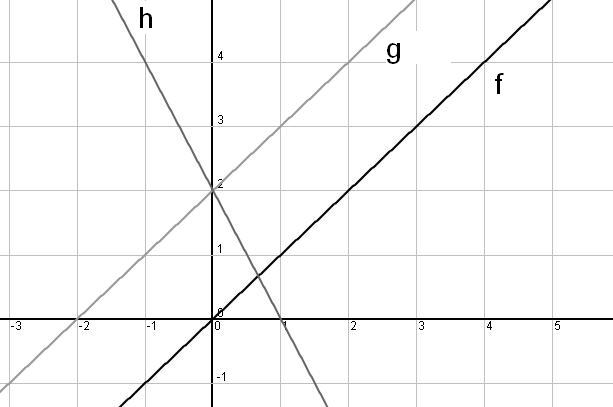
\includegraphics[width=.6\textwidth]{img/LinF.jpg}

\section*{Quadratische Funktionen}
\subsection*{Allgemeine Form: $y= ax^2 + bx + c$}
\begin{itemize}
	\item \textbf{Definitionsbereich}: $ D = \mathbb{R} $
	\item \textbf{Wertebereich für $a>0$}: $ W = [\frac{4ac-b^2}{4a}, +\infty) $
	\item \textbf{Wertebereich für $a<0$}: $ W = (-\infty, \frac{4ac-b^2}{4a}] $
	\item \textbf{Nullstelle}: $ x_{1,2} \ = \ \frac {-b \ \pm \ \sqrt{b^2 \ - \ 4ac}} {2a} $
	\item \textbf{Scheitelpunkt}: $ x_{1,2} \ = \ S(-\frac{b}{2a}, \frac{4ac-b^2}{4a} )$
\end{itemize}

\subsection*{Normalform $y = x^2 + px + q$}
\begin{itemize}
	\item \textbf{Definitionsbereich}: $ D = \mathbb{R} $
	\item \textbf{Wertebereich}: $ W = [q-\frac{p^2}{4}, +\infty) $
	\item \textbf{Nullstelle}: $ x_{1, 2}= - \frac{p}{2} \pm
\sqrt{\frac{p^2}{a}-q} $
	\item \textbf{Scheitelpunkt}: $ S(-\frac{p}{2}, -\frac{p^2}{4}+q )$
	\item \textbf{Spezialfall}: $y = (x+d)^2 +e $
	\item \textbf{Graph}: \\
		$f$: $a=\frac 1 2$, $b=-2$, $c=2$; \\
		$g$: $a=1$, $b=0$, $c=0$; \\
		$h$: $a=-4$, $b=0$, $c=-\frac 1 2$ \\
\end{itemize}
%\textbf{Graph}: \\
%		$f$: $a=\frac 1 2$, $b=-2$, $c=2$; \\
%		$g$: $a=1$, $b=0$, $c=0$; \\
%		$h$: $a=-4$, $b=0$, $c=-\frac 1 2$ \\
	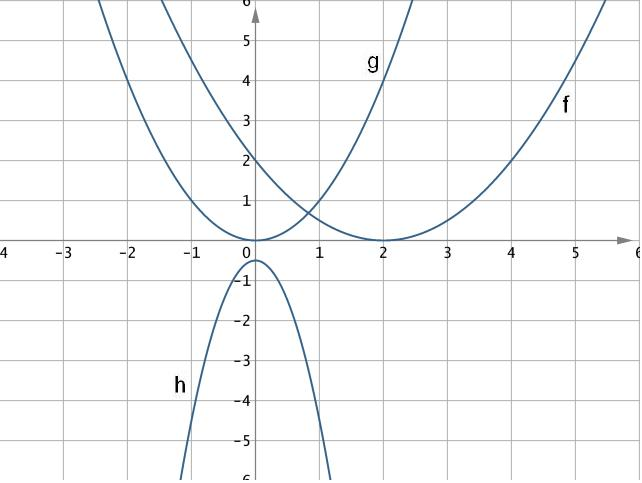
\includegraphics[width=.6\textwidth]{img/QuadFkt.jpg}

\section*{Potenzfunktionen $ y = f(x) = x^n $}

\subsection*{Positiver gerader Exponent\\ $n = 2m$ mit $ m \in \mathbb{N}-\{0\}$}
\begin{itemize}
	\item \textbf{Definitionsbereich}: $ D = \mathbb{R} $
	\item \textbf{Wertebereich}: $ W = [0, + \infty) $
	\item \textbf{Nullstelle}: $ x_0 = 0 $
	\item \textbf{gemeinsame Punkte}: $(-1;1), (0;0), (1;1) $
	\item \textbf{Graph}: $f$: $n=2$; $g$: $n=4$; $h$: $n=8$ \\ 
\begin{center}
	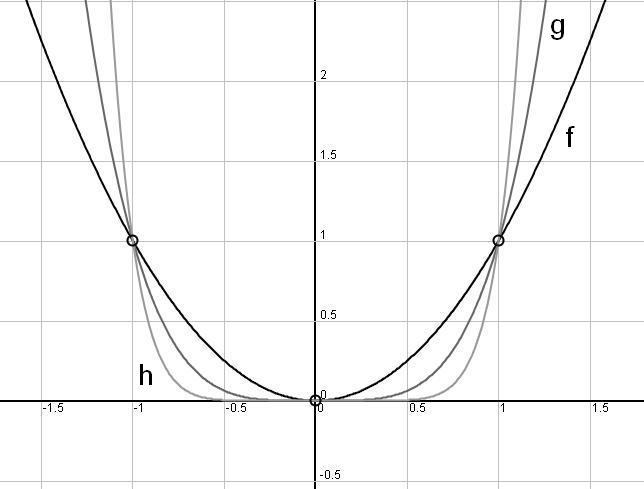
\includegraphics[width=0.60\textwidth]{img/P1.jpg}
\end{center}
\end{itemize}

\subsection*{Positiver ungerader Exponent\\ $n = 2m+1$ mit $ m \in \mathbb{N}-\{0\}$}
\begin{minipage}{.5\textwidth}
\begin{itemize}
	\item \textbf{Definitionsbereich}: $ D = \mathbb{R} $
	\item \textbf{Wertebereich}: $ W = \mathbb{R} $
	\item \textbf{Nullstelle}: $ x_0 = 0 $
	\item \textbf{gemeinsame Punkte}:\\ $(-1;-1), (0;0), (1;1) $
	\item \textbf{Graph}: $f$: $n = 3$; $g$: $n=9$ \\
\end{itemize}
\end{minipage}
\begin{minipage}{.5\textwidth}
		\includegraphics[height=4cm]{img/P2.jpg}
\end{minipage}


\subsection*{Negativer gerader Exponent\\ $n = -2m$ mit $ m \in \mathbb{N}-\{0\}$}
\begin{itemize}
	\item \textbf{Definitionsbereich}: $ D = \mathbb{R}-\{0\} $
	\item \textbf{Wertebereich}: $ W = (0, + \infty) $
	\item \textbf{Nullstelle}: keine
	\item \textbf{gemeinsame Punkte}: $(-1;1), (1;1) $
	\item \textbf{Graph}:$f$: $n = -2$; $g$: $n=-8$ \\
\begin{center}
		\includegraphics[width=0.60\textwidth]{img/P3.jpg}
\end{center}
\end{itemize}

\subsection*{Negativer ungerader Exponent\\ $n = -(2m+1)$ mit $ m \in \mathbb{N}-\{0\}$}
\begin{itemize}
	\item \textbf{Definitionsbereich}: $ D = \mathbb{R}-\{0\} $
	\item \textbf{Wertebereich}: $ W = \mathbb{R}-\{0\} $
	\item \textbf{Nullstelle}: keine
	\item \textbf{gemeinsame Punkte}: $(-1;-1), (1;1) $
	\item \textbf{Graph}:$f$: $n = -3$; $g$: $n=-9$ \\
\begin{center}
		\includegraphics[width=0.60\textwidth]{img/P4.jpg}
\end{center}
\end{itemize}

\section*{Wurzelfunktionen $y = x^n $ mit $ n = \frac{p}{q}$ \\ ($p$, $q \in \mathbb{N}-\{0\}$, $ q $ teilt $ p $ nicht) }
\begin{itemize}
	\item \textbf{Definitionsbereich}: $ D = [0, +\infty) $
	\item \textbf{Wertebereich}: $ W = [0, +\infty) $
	\item \textbf{Nullstelle}: $x_0 = 0 $
	\item \textbf{gemeinsame Punkte}: $(0;0), (1;1) $
	\item \textbf{Graph}:$f$: $n = \frac{1}{2}$; $g$: $n=\frac{1}{4}$ \\
\begin{center}
		\includegraphics[width=0.60\textwidth]{img/WurzelF.jpg}
\end{center}
\end{itemize}

\section*{Winkelfunktionen}

\subsection*{Sinusfunktion $ y = \sin x $}
\begin{itemize}
	\item \textbf{Definitionsbereich}: $ D = \mathbb{R} $
	\item \textbf{Wertebereich}: $ W = [-1, +1] $
	\item \textbf{Nullstelle}: $x_k = k\pi $, $k \in \mathbb{Z}$
	\item \textbf{Periode}: $2\pi$
	\item \textbf{Graph}: \\
\begin{center}
		\includegraphics[width=0.60\textwidth]{img/SinF1.jpg}
\end{center}
\end{itemize}

\subsection*{Sinusfunktion $ y = a \sin (bx + c) $ \\ mit $ a $, $c \in \mathbb{R}$, $b \in \mathbb{R}-\{0\}$}
\begin{itemize}
	\item \textbf{Definitionsbereich}: $ D = \mathbb{R} $
	\item \textbf{Wertebereich}: $ W = [-a, +a] $
	\item \textbf{Nullstelle}: $x_k =  \frac{k\pi - c}{b} $, $k \in \mathbb{Z}$
	\item \textbf{Periode}: $\frac{2\pi}{b}$
	\item \textbf{Verschiebung in x-Richtung}: Verschiebung um $\frac{c}{b}$ ($> 0$) in negativer x-Richtung
	\item \textbf{Graph}:$f$: $a = 2$, $b=1$, $c=0$; $g$: $a=1$, $b=2$, $c=0$; $h$: $a=1$, $b=2$, $c=\pi$ \\
\begin{center}
		\includegraphics[width=0.60\textwidth]{img/SinF2.jpg}
\end{center}
\end{itemize}

\subsection*{Kosinusfunktion $y = \cos x$}
\begin{itemize}
	\item \textbf{Definitionsbereich}: $ D = \mathbb{R} $
	\item \textbf{Wertebereich}: $ W = [-1, +1] $
	\item \textbf{Nullstelle}: $x_k = (2k + 1)\frac{\pi}{2} $, $k \in \mathbb{Z}$
	\item \textbf{Periode}: $2\pi$
	\item \textbf{Graph}: \\
\begin{center}
		\includegraphics[width=0.60\textwidth]{img/CosF.jpg}
\end{center}
\end{itemize}

\subsection*{Tangensfunktion $y = \tan x$}
\begin{itemize}
	\item \textbf{Definitionsbereich}: $ D = \mathbb{R}-\{(2k+1)\frac{\pi}{2} : k \in \mathbb{Z}\} $
	\item \textbf{Wertebereich}: $ W = \mathbb{R} $
	\item \textbf{Nullstelle}: $x_k = k\pi $, $k \in \mathbb{Z}$
	\item \textbf{Periode}: $\pi$
	\item \textbf{Graph}: \\
\begin{center}
		\includegraphics[width=0.60\textwidth]{img/TanF.jpg}
\end{center}
\end{itemize}

\subsection*{Arkussinusfunktion $y = \arcsin x$}
\begin{minipage}{.5\textwidth}
\begin{itemize}
	\item \textbf{Definitionsbereich}: $ D = [-1, 1] $
	\item \textbf{Wertebereich}: $ W = [-\frac{\pi}{2}, \frac{\pi}{2}] $
	\item \textbf{Nullstelle}: $x_0 = 0$
\end{itemize}
\end{minipage}
\begin{minipage}{.5\textwidth}
		\includegraphics[height=3cm]{img/ASinF.jpg}
\end{minipage}


\subsection*{Arkuscosinusfunktion $y = \arccos x$}
\begin{minipage}{.5\textwidth}
\begin{itemize}
	\item \textbf{Definitionsbereich}: $ D = [-1, 1] $
	\item \textbf{Wertebereich}: $ W = [0, \pi] $
	\item \textbf{Nullstelle}: $x_0 = 1$
\end{itemize}
\end{minipage}
\begin{minipage}{.5\textwidth}	
\includegraphics[height=3cm]{img/ACosF.jpg}
\end{minipage}

\subsection*{Arkustangensfunktion $y = \arctan x$}
\begin{minipage}{.5\textwidth}
\begin{itemize}
	\item \textbf{Definitionsbereich}: $ D = \mathbb{R} $
	\item \textbf{Wertebereich}: $ W = [-\frac{\pi}{2}, \frac{\pi}{2}] $
	\item \textbf{Nullstelle}: $x_0 = 0$
\end{itemize}
\end{minipage}
\begin{minipage}{.5\textwidth}
		\includegraphics[width=\textwidth]{img/ATanF.jpg}
\end{minipage}

\newpage
\section*{Exponentialfunktionen $y = a^x$ \\ mit $a \in \mathbb{R_+}-\{1\}$}
\begin{minipage}{.5\textwidth}
\begin{itemize}
	\item \textbf{Definitionsbereich}: $ D = \mathbb{R} $
	\item \textbf{Wertebereich}: $ W = (0, + \infty) $
	\item \textbf{Nullstelle}: keine
	\item \textbf{gemeinsamer Punkt}: $(0;1)$
	\item \textbf{Graph} für $a = \tfrac{1}{2}, 10, e$:
\end{itemize} 
\end{minipage}
\begin{minipage}{.5\textwidth}
\includegraphics[height=4cm]{img/exp.pdf} 
\end{minipage}

\section*{Logarithmusfunktionen $y = \log_a x$ \\ mit $a \in
\mathbb{R_+}-\{1\}$}

\begin{minipage}{.5\textwidth}
\begin{itemize}
	\item \textbf{Definitionsbereich}: $ D = (0, + \infty) $
	\item \textbf{Wertebereich}: $ W = \mathbb{R} $
	\item \textbf{Nullstelle}: $ x_0 = 1 $
	\item \textbf{gemeinsamer Punkt}: $(1;0)$
	\item \textbf{Graph} für $a= e, 10, \tfrac{1}{2}$:
\end{itemize}
\end{minipage}
\begin{minipage}{.5\textwidth}
\includegraphics[height=4cm]{img/log.pdf}
\end{minipage}


%\section*{Literatur}
%Formeln und Tabellen für die Sekudarstufen I und II. 7. Aufl. - Berlin: Paetec, Ges. für %Bildung und Technik, 1999


%\include{ZusammenfassungKay}
%\section{Komplexe Zahlen}

komplexe Zahlen:
\;$\displaystyle
\complex
\ =\ \{\;x+\imag y\;|\;x,y\in\real\;\}
\,.
$

kartesische Darstellung: $z=x+\imag y$,
\\
Realteil $\re(z)=x$, Imaginärteil $\im(z)=y$

Eulersche Darstellung: $z=r\e^{\imag\varphi}$,
\\
Betrag $\abs{z}=r\ge0$, Hauptargument $\arg{z}=\varphi\in\ocinterval{-\pi}{\pi}$

Zusammenhang: $r\e^{\imag\varphi}=r\,(\cos\varphi+\imag\sin\varphi)$, wobei $r=\sqrt{x^2+y^2}$ und $\varphi=\arctan(y/x)$ aus richtigem Quadranten:
\[
\begin{array}{c|c|c}
x & y & \varphi=\\
\hline
\ge0 & =0 & 0\\
<0 & =0 & \pi\\
=0 & >0 & \pi/2\\
=0 & <0 & -\pi/2
\end{array}
\qquad
\begin{array}{c|c|c}
x & y & \varphi\in\\
\hline
>0 & >0 & \ointerval{0}{\pi/2}\\
>0 & <0 & \ointerval{-\pi/2}{0}\\
<0 & >0 & \ointerval{\pi/2}{\pi}\\
<0 & <0 & \ointerval{-\pi}{-\pi/2}
\end{array}
\]
und umgekehrt: $x=r\cos\varphi$ und $y=r\sin\varphi$

konjugiert komplexe Zahl: $z=x-\imag y$

Addition: $(a+\imag b)+(c+\imag d)=(a+c)+\imag(b+d)$

Subtraktion: $(a+\imag b)-(c+\imag d)=(a-c)+\imag(b-d)$

Multiplikation: $(a+\imag b)\cdot(c+\imag d)=(ac-bd)+\imag(bc+ad)$
\\
bzw.\ $r\e^{\imag\varphi}\cdot{}s\e^{\imag\psi}=(rs)\,\e^{\imag(\varphi+\psi)}$

Division (erweitern mit konjugiert Komplexem des Nenners):
\\
$\displaystyle\frac{a+\imag b}{c+\imag d}
=\frac{ac+bd}{c^2+d^2}+\imag\,\frac{bc-ad}{c^2+d^2}$
\\
bzw.\ $\displaystyle\frac{r\e^{\imag\varphi}}{s\e^{\imag\psi}}
=\frac{r}{s}\,\e^{\imag(\varphi-\psi)}$ für $s>0$

Potenzen von $\imag$: Für $n\in\integer$ ist
\[
\imag^n
\ =\ \left\{\begin{array}{r@{\,,\; \text{falls}\quad}l}
1      & n\equiv0\!\mod4\\
\imag  & n\equiv1\!\mod4\\
-1     & n\equiv2\!\mod4\\
-\imag & n\equiv3\!\mod4
\end{array}\right.
\]
Potenzieren mit Exponenten $a\in\real$:
$
z^a=r^a\,\e^{\imag(a\varphi+2ak\pi)}
$
\\
und falls $a\in\integer$ speziell
$
z^a=r^a\,\e^{\imag a\varphi}
$

Radizieren: $n$-ten Wurzeln für $n=2,3,\dotsc$,
\[
\sqrt[n]{r}\,\left(
\cos\frac{\varphi+2k\pi}n
+\imag\sin\frac{\varphi+2k\pi}n
\right)
,\quad{}
k=0,\dotsc,n-1
\,,
\]
teilen den Kreis um Nullpunkt mit Radius $\sqrt[n]{r}$ in $n$ gleiche Teile

%================================================================================
\section{Kurvendiskussion}

Definitionsbereich: $D(f)$, Wertebereich: $W(f)=\{f(x)\,|\,x\in{}D(f)\}$

Definitionslücken? Stetigkeit? Differenzierbarkeit?

Nullstellen: $f(x_0)=0$

Extrema: $f'(x_{\e})=0$ und dann
\\
lokales Minimum: $f''(x_{\e})>0$, lokales Maximum: $f''(x_{\e})<0$
\\
globale Extrema: betrachte zusätzlich $\lim\limits_{x\to-\infty}f(x)$ und
$\lim\limits_{x\to\infty}f(x)$

Monotonie: wachsend: $f'(x)>0$, fallend: $f'(x)<0$

Krümmung: konvex: $f''(x)>0$, konkav: $f''(x)<0$

Wendestelle: $f''(x_{\w})=0$ und $f'''(x_{\w})\neq0$

weiteres: Polstellen? Asymptoten? Periodizität?

Skizzieren des Graphen!


\end{document}
